%%%%%%%%%%%%%%%%%%%%%%%%%%%%%%%%%%%%%%%%%%%%%%%%%%%%%%%%%%%%%%%%%%%%%%%%%%%
% Plantilla genérica para TFG/TFM/Tesis.
%
% Función: documento principal.
%
% Uso: compila este fichero. Normalmente no necesitas modificarlo:
% configura Config/myconfig.tex y organiza los capítulos y apéndices en
% content-standard.tex o content-compendium.tex.
%
% Autores: Javier Macías-Guarasa (UAH), Roberto Barra-Chicote (UPM, Amazon).
%
% Basada en fuentes de Roberto Barra, Manuel Ocaña, Jesús Nuevo,
% Pedro Revenga, Fernando Herránz y Noelia Hernández.
% Adaptación original para la URJC: Rubén Nieto Capuchino.
% Otros colaboradores: Book/additionalContributors.txt.
%
% Tus mejoras y sugerencias son bienvenidas:
% javier.maciasguarasa@uah.es
%%%%%%%%%%%%%%%%%%%%%%%%%%%%%%%%%%%%%%%%%%%%%%%%%%%%%%%%%%%%%%%%%%%%%%%%%%%

% The document language is selected from myconfig.tex and loaded through
% Babel in Config/postamble.tex. Do not hard-code a language at class level.
\documentclass[openright]{book}

%%%%%%%%%%%%%%%%%%%%%%%%%%%%%%%%%%%%%%%%%%%%%%%%%%%%%%%%%%%%%%%%%%%%%%%%%%%
% BEGIN Preamble and configuration section
%
%%%%%%%%%%%%%%%%%%%%%%%%%%%%%%%%%%%%%%%%%%%%%%%%%%%%%%%%%%%%%%%%%%%%%%%%%%% 
% 
% Generic template for TFC/TFM/TFG/Tesis
% 
% $Id: preamble.tex,v 1.34 2017/04/06 13:56:12 macias Exp $
% 
% By:
% + Javier Macías-Guarasa. 
%   Departamento de Electrónica
%   Universidad de Alcalá
% + Roberto Barra-Chicote. 
%   Departamento de Ingeniería Electrónica
%   Universidad Politécnica de Madrid   
% 
% Based on original sources by Roberto Barra, Manuel Ocaña, Jesús Nuevo,
% Pedro Revenga, Fernando Herránz and Noelia Hernández. Thanks a lot to
% all of them, and to the many anonymous contributors found (thanks to
% google) that provided help in setting all this up.
% 
% See also the additionalContributors.txt file to check the name of
% additional contributors to this work.
% 
% If you think you can add pieces of relevant/useful examples,
% improvements, please contact us at (macias@depeca.uah.es)
% 
% You can freely use this template and please contribute with
% comments or suggestions!!!
% 
%%%%%%%%%%%%%%%%%%%%%%%%%%%%%%%%%%%%%%%%%%%%%%%%%%%%%%%%%%%%%%%%%%%%%%%%%%% 

% Make sure synctex is active
\synctex=1

%% This is used in anteproyecto
\usepackage{pgfgantt}

% To allow changing the default alignment of an image
\usepackage[export]{adjustbox}

% To allow simple notes to be used in the review process (see defined
% commands at the end of this file)
\usepackage{todonotes} 

% ifthen to allow using language dependent settings
\usepackage{ifthen}

%% JMG: FIXING PROBLEM WITH ALL PAGES PRINTED IN COLOR
% This should not be touched, as it should work as it is know.
\newcommand{\colorspaceused}{rgb}

% The next section seems to be useless, but it's still pending to try further
\ifthenelse{\equal{\colorspaceused}{rgb}}
{
  \PassOptionsToPackage{rgb}{xcolor}% NB: put this *before* \usepackage{pst-all}
}
{
  \PassOptionsToPackage{cmyk}{xcolor}% NB: put this *before* \usepackage{pst-all}
}

\usepackage{iftex}
\ifPDFTeX
  \usepackage[utf8]{inputenc}   % To allow writing accented characters , ñ, etc.
  \usepackage[T1,TS1]{fontenc}  % To properly handle ``hyphenation''. Do not use as it
\fi                             %  significantly slows compilation down
\usepackage{ae}                 % For all fonts to be Type1, and none Type3.
\usepackage{lmodern}            % This generates a pdf with searchable
                                %  accented characters!!!!!!!!!!!!!!!!!!!!!!!!!!!!!!!!!!!!!!!
\usepackage{textcomp}

\usepackage{wrapfig}
\usepackage{lipsum}

% Use this if you want to include pdf files in the final document
\usepackage[final]{pdfpages}

% Use this if you want to delete headers and footers in empty pages
\usepackage{emptypage}

% \usepackage[nottoc]{tocbibind}
\usepackage{tocbibind}

\usepackage{listings}
\usepackage{longtable}
\usepackage{afterpage}

\usepackage{xspace}
\usepackage{verbatim}
\usepackage{moreverb}
\usepackage{multicol}
\usepackage{amsmath}
\usepackage{eurosym}
% \usepackage{subfig} % subfigure is obsolete...
\usepackage{multirow}
\usepackage{fancyhdr}
\usepackage{makeidx}
\usepackage{rotating}
%\usepackage{supertabular}
\usepackage{hhline}
\usepackage{array}



%% FIXING PROBLEM WITH ALL PAGES PRINTED IN COLOR
\usepackage{xcolor}
\providecommand{\myConfigDirectory}{../Config}
\input{\myConfigDirectory/colors.tex}


% To draw rectagles in tfm cover
\usepackage{tikz}

\usepackage{geometry}
\geometry{verbose,a4paper,tmargin=2.5cm,bmargin=2.5cm,lmargin=2.5cm,rmargin=2.5cm}

\usepackage{hyperref}
\usepackage{hyperxmp}
\hypersetup{
  %% ps2pdf,                         %%% hyper-references for ps2pdf
  bookmarks=true,%                   %%% generate bookmarks ...
  bookmarksnumbered=true,            %%% ... with numbers
  hypertexnames=false,               %%% needed for correct links to figures!!!
  % hypertexnames=true,              %%% needed for correct links on pagebackrefs!!!
  breaklinks=true,                   %%% breaks lines, but links are very small
  % pagebackref=true,
  % linktocpage=true,                %%% Link in the page number
  linktoc=all,
  colorlinks=true,
  linkcolor=blue,
  citecolor=green,
  urlcolor=blue,                     %%% text with color (further
                                     %%%  modified in myconfig.tex)
  % linkbordercolor={0 0 1},         %%% blue frames around links
  pdfborder={0 0 112.0},             %%% border-width of frames
  hyperfootnotes=false
}                        %%% will be multiplied with 0.009 by ps2pdf


% JMG 03/2025: This section tries to allow the use of a single preamble.tex, by
% checking if chapter is defined. Chapter should be defined when compiling
% book.tex, and not otherwise (for example in anteproyecto.tex).
% So, the strategy is checking if chapter is defined:
% - If it is, assume it is compiling book.tex and include all elements that generate
%   errors in other tex files
% - If if is not, assume we are compiling other than book.tex, and define anything
%   required that can generates in the packages being used below
\makeatletter
\@ifundefined{chapter} % This happens if compiling anteproyecto.tex. Dirty but...
{
  % Define this to avoid complains in packages included later
  \newcounter{chapter}
  \newcommand{\chaptermark}[1]{\markboth{#1}{}}
  % This should be relative to the anteproyecto path
  \newcommand{\myreferencespath}{../Book/}

}
{
  % JMG 03/2025 It is included here to avoid compilation errors in
  % anteproyecto.tex. This is dirty, I know

  % glossaries is better than the acronym package
  \usepackage[automake,acronym,shortcuts,nomain,hyperfirst=false]{glossaries}
  % If you want to PERMANENTLY DISABLE HYPERLINKS, uncomment the following
  % line
  % \glsdisablehyper
  % In future versiones (not as for ubuntu 12.04) You can also selectively
  % disable hyperlinks for given glossaries, using:
  % \usepackage[acronym,shortcuts,nomain,nohypertypes={acronyms,symbols}]{glossaries}
  % Or (for newwer versions also), you can even use
  % \GlsDeclareNoHyperList{acronyms,symbols}
  % You can also disable hyperlinks in the acronym use, like in \ac*{symbol}

  % This should be relative to the book.tex path, do not touch!!!!!!!!!!!
  \newcommand{\myreferencespath}{}

}
\makeatother


% \usepackage[all]{hypcap}
\usepackage[center]{caption}
\usepackage{subcaption}


% Para numerar las \subsubsection
\setcounter{secnumdepth}{5}
% para hacer que las \subsubsection aparezcan en el indice
\setcounter{tocdepth}{5}
% \setcounter{lofdepth}{2}
\setcounter{table}{1}
\setcounter{figure}{1}
\setcounter{secnumdepth}{4}

\setlength{\parskip}{1ex plus 0.5ex minus 0.2ex}

\usepackage{multirow}

\usepackage{setspace}

\newcommand{\mycaptiontable}[1]{
  \begin{spacing}{0.6}
    % \vspace{0.5cm}
    \begin{quote}
      % \begin{center}
      {{Table} \thechapter.\arabic{table}: #1}
      % \end{center}
    \end{quote}
    % \vspace{1cm}
  \end{spacing}
  \stepcounter{table}
}

\newcommand{\mycaptionfigure}[1]{
  % \vspace{0.5cm}
  \begin{spacing}{0.6}
    \begin{quote}
      % \begin{center}
      {{Figure} \thechapter.\arabic{figure}: #1}
      % \end{center}
    \end{quote}
    % \vspace{1cm}
  \end{spacing}
  \stepcounter{figure}
}

\usepackage{amsmath}

\usepackage{courier}

% ***************************************************************************
% ***************************************************************************
% ***************************************************************************
\usepackage{multirow}
\usepackage{rotating}
\usepackage{setspace, amssymb, amsmath, epsfig, multirow, colortbl, tabularx}%

\newcommand{\clearemptydoublepage}{\newpage{\pagestyle{empty}\cleardoublepage}}

\pagestyle{fancy}

\providecommand\phantomsection{}
\onehalfspacing
\sloppy  %better line breaks

\renewcommand{\chaptermark}[1]{\markboth{\chaptername\ \thechapter.\ #1}{}}
\renewcommand{\sectionmark}[1]{\markright{\thesection\ #1}{}}

%%%%%%%%%%%%%%%%%%%%%%%%%%%%%%%%%%%%%%%%%%%%%%%%%%%%%%%%%%%%%%%%%%%%%%%%%%% 
% BEGIN Fancy headers stuff
\fancyhf{}

\fancyhead[LE,RO]{\bfseries\thepage}
\fancyhead[LO]{\bfseries\rightmark}
\fancyhead[RE]{\bfseries\leftmark}

\makeatletter
\renewcommand{\chaptermark}[1]{\markboth{\@chapapp \ \thechapter . \ #1}{}}
\renewcommand{\sectionmark}[1]{\markright{\thesection \ \ #1}}
\makeatother

\renewcommand{\headrulewidth}{0.5pt}
\renewcommand{\footrulewidth}{0pt}
\addtolength{\headheight}{3.5pt}
\fancypagestyle{plain}{\fancyhead{}\renewcommand{\headrulewidth}{0pt}}
\fancypagestyle{myplain}
{
  \fancyhf{}
  \renewcommand\headrulewidth{0pt}
  \renewcommand\footrulewidth{0pt}
  \fancyfoot[C]{\thepage}
}
% END Fancy headers stuff
%%%%%%%%%%%%%%%%%%%%%%%%%%%%%%%%%%%%%%%%%%%%%%%%%%%%%%%%%%%%%%%%%%%%%%%%%%% 

%%%%%%%%%%%%%%%%%%%%%%%%%%%%%%%%%%%%%%%%%%%%%%%%%%%%%%%%%%%%%%%%%%%%%%%%%%% 
% BEGIN Set nice chapter titles

% BEGIN Example 0 from http://texblog.org/2012/07/03/fancy-latex-chapter-styles/
% \usepackage[explicit]{titlesec}
% \usepackage{blindtext}
% \definecolor{gray75}{gray}{0.75}
% \newcommand{\hsp}{\hspace{20pt}}
% \titleformat{\chapter}[hang]{\Huge\bfseries}{\chaptername~\thechapter\hsp\textcolor{gray75}{|}\hsp}{0pt}{\Huge\bfseries}
% END Example 0 from http://texblog.org/2012/07/03/fancy-latex-chapter-styles/

% BEGIN Example 1 from http://texblog.org/2012/07/03/fancy-latex-chapter-styles/
% \usepackage{titlesec}
% \usepackage{blindtext}
% \definecolor{gray75}{gray}{0.75}
% \newcommand{\hsp}{\hspace{20pt}}
% \titleformat{\chapter}[hang]{\Huge\bfseries}{\chaptername~\thechapter\hsp\textcolor{gray75}{|}\hsp}{0pt}{\Huge\bfseries}
% END Example 1 from http://texblog.org/2012/07/03/fancy-latex-chapter-styles/

% BEGIN Example 2 from http://texblog.org/2012/07/03/fancy-latex-chapter-styles/
% Options: Sonny, Lenny, Glenn, Conny, Rejne, Bjarne, Bjornstrup
% \usepackage[Sonny]{fncychap}
% \usepackage[Lenny]{fncychap} % ugly
% \usepackage[Glenn]{fncychap}
% \usepackage[Conny]{fncychap} % ugly
% \usepackage[Rejne]{fncychap}
% \usepackage[Bjarne]{fncychap} % Doesn't work in Spanish
% \usepackage[Bjornstrup]{fncychap}
% END   Example 2 from http://texblog.org/2012/07/03/fancy-latex-chapter-styles/

% BEGIN Example 3 from http://texblog.org/2012/07/03/fancy-latex-chapter-styles/
% This is a nice colored example
% \usepackage{kpfonts}
% \usepackage[explicit]{titlesec}
% \newcommand*\chapterlabel{}
% \titleformat{\chapter}
% {\gdef\chapterlabel{}
% \normalfont\sffamily\Huge\bfseries\scshape}
% {\gdef\chapterlabel{\thechapter\ }}{0pt}
% {\begin{tikzpicture}[remember picture,overlay]
%   \node[yshift=-3cm] at (current page.north west)
%   {\begin{tikzpicture}[remember picture, overlay]
%     \draw[fill=LightSkyBlue] (0,0) rectangle
%     (\paperwidth,3cm);
%     \node[anchor=east,xshift=.9\paperwidth,rectangle,
%     rounded corners=20pt,inner sep=11pt,
%     fill=MidnightBlue]
%     {\color{white}\chapterlabel#1};
%   \end{tikzpicture}
% };
% \end{tikzpicture}
% }
%   \titlespacing*{\chapter}{0pt}{50pt}{-60pt}
%   END   Example 3 from http://texblog.org/2012/07/03/fancy-latex-chapter-styles/

%   BEGIN Example 4 from http://texblog.org/2012/07/03/fancy-latex-chapter-styles/
%   END   Example 4 from http://texblog.org/2012/07/03/fancy-latex-chapter-styles/


%   END Set nice chapter titles
%%%%%%%%%%%%%%%%%%%%%%%%%%%%%%%%%%%%%%%%%%%%%%%%%%%%%%%%%%%%%%%%%%%%%%%%%%%   

%%%%%%%%%%%%%%%%%%%%%%%%%%%%%%%%%%%%%%%%%%%%%%%%%%%%%%%%%%%%%%%%%%%%%%%%%%%   
%   This is to set background images (in our case to set background image
%   in TFMs front and back pages)
%   If you want to set this background, use \BgThispage in the
%   corresponding pages
%   \usepackage[pages=some]{sty/background}
\usepackage[pages=some]{background}

% This is to allow do a clearpage and let the next one to be placed in
% even pages (to set a backpage for example)
\makeatletter
\newcommand*{\cleartoleftpage}{%
  \clearpage
  \if@twoside
    \ifodd\c@page
      \hbox{}\newpage
      \if@twocolumn
        \hbox{}\newpage
      \fi
    \fi
  \fi
}
\makeatother

% Let's define some styles for source code listings:
% 
% This was using the float package
\usepackage{float}
\floatstyle{plaintop} % optionally change the style of the new float
\newfloat{codefloat}{H}{cod}[chapter]

% Support utf-8 in listings. 
% The way the inputenc package works with non-ASCII UTF-8-encoded characters (by
% making the first byte active and then reading the following ones as arguments)
% is fundamentally incompatible with the way the listing package works, which
% reads each byte individually and expects it to be an individual character.
% See https://tex.stackexchange.com/questions/24528/having-problems-with-listings-and-utf-8-can-it-be-fixed
\lstset{
  inputencoding = utf8,  % Input encoding
  extendedchars = true,  % Extended ASCII
  literate      =        % Support additional characters
  {á}{{\'a}}1  {é}{{\'e}}1  {í}{{\'i}}1 {ó}{{\'o}}1  {ú}{{\'u}}1
  {Á}{{\'A}}1  {É}{{\'E}}1  {Í}{{\'I}}1 {Ó}{{\'O}}1  {Ú}{{\'U}}1
  {à}{{\`a}}1  {è}{{\`e}}1  {ì}{{\`i}}1 {ò}{{\`o}}1  {ù}{{\`u}}1
  {À}{{\`A}}1  {È}{{\'E}}1  {Ì}{{\`I}}1 {Ò}{{\`O}}1  {Ù}{{\`U}}1
  {ä}{{\"a}}1  {ë}{{\"e}}1  {ï}{{\"i}}1 {ö}{{\"o}}1  {ü}{{\"u}}1
  {Ä}{{\"A}}1  {Ë}{{\"E}}1  {Ï}{{\"I}}1 {Ö}{{\"O}}1  {Ü}{{\"U}}1
  {â}{{\^a}}1  {ê}{{\^e}}1  {î}{{\^i}}1 {ô}{{\^o}}1  {û}{{\^u}}1
  {Â}{{\^A}}1  {Ê}{{\^E}}1  {Î}{{\^I}}1 {Ô}{{\^O}}1  {Û}{{\^U}}1
  {œ}{{\oe}}1  {Œ}{{\OE}}1  {æ}{{\ae}}1 {Æ}{{\AE}}1  {ß}{{\ss}}1
  {ç}{{\c c}}1 {Ç}{{\c C}}1 {ø}{{\o}}1  {Ø}{{\O}}1   {å}{{\r a}}1
  {Å}{{\r A}}1 {ã}{{\~a}}1  {õ}{{\~o}}1 {Ã}{{\~A}}1  {Õ}{{\~O}}1
  {ñ}{{\~n}}1  {Ñ}{{\~N}}1  {¿}{{?`}}1  {¡}{{!`}}1
  {°}{{\textdegree}}1 {º}{{\textordmasculine}}1 {ª}{{\textordfeminine}}1
  % ¿ and ¡ are not correctly displayed if inconsolata font is used
  % together with the lstlisting environment. Consider typing code in
  % external files and using \lstinputlisting to display them instead.
}

\lstdefinestyle{console}
{
  basicstyle=\scriptsize\bf\ttfamily,
  backgroundcolor=\color{gray75},
}

\lstdefinestyle{Cbluebox}
{
  language=C,
  frame=shadowbox, 
  rulesepcolor=\color{blue}
}

\lstdefinestyle{Cnice}
{
  language=C,
  frame=Ltb,
  framerule=0pt,
  tabsize=2,
  aboveskip=0.5cm,
  framextopmargin=3pt,
  framexbottommargin=3pt,
  framexleftmargin=0.4cm,
  framesep=0pt,
  rulesep=.4pt,
  backgroundcolor=\color{gray97},
  rulesepcolor=\color{black},
  % 
  stringstyle=\ttfamily,
  showstringspaces = false,
  % basicstyle=\small\ttfamily,
  basicstyle=\footnotesize\ttfamily,
  commentstyle=\color{gray45},
  keywordstyle=\bfseries,
  % 
  numbers=left,
  numbersep=15pt,
  numberstyle=\tiny,
  numberfirstline = false,
  breaklines=true,
}	

\lstdefinestyle{CppExample}
{
  language=C++,
  frame=trbl,
  tabsize=2,
  commentstyle=\textit,
  stringstyle=\ttfamily, 
  basicstyle=\small,
}	

% This one from http://en.wikibooks.org/wiki/LaTeX/Source_Code_Listings
\lstdefinestyle{Ccolor}
{
  belowcaptionskip=1\baselineskip,
  breaklines=true,
  frame=L,
  xleftmargin=\parindent,
  language=C,
  showstringspaces=false,
  basicstyle=\footnotesize\ttfamily,
  keywordstyle=\bfseries\color{green!40!black},
  commentstyle=\itshape\color{purple!40!black},
  identifierstyle=\color{blue},
  stringstyle=\color{orange},
}

% From http://tex.stackexchange.com/questions/46953/unix-command-highlighting-latex
\lstdefinestyle{BashInputStyle}{
  language=bash,
  basicstyle=\small\sffamily,
  numbers=left,
  numberstyle=\tiny,
  numbersep=3pt,
  frame=tb, 
  showspaces=false, 
  showtabs=false,
  showstringspaces=false,
  columns=fullflexible,
  backgroundcolor=\color{gray97},
  % backgroundcolor=\color{yellow!20},
  linewidth=0.9\linewidth,
  xleftmargin=0.05\linewidth
}


% To set side-captions in figures
\usepackage{sidecap}

%%%%%%%%%%%%%%%%%%%%%%%%%%%%%%%%%%%%%%%%%%%%%%%%%%%%%%%%%%%%%%%%%%%%%%%%%%% 
% This comes from TeXiS, thanks to its authors, available at
% http://gaia.fdi.ucm.es/projects/texis 
\def\texis{\TeX \raise.15em\hbox{\textsc{i}}S}
%%%%%%%%%%%%%%%%%%%%%%%%%%%%%%%%%%%%%%%%%%%%%%%%%%%%%%%%%%%%%%%%%%%%%% 
% Comando:
% 
% \begin{FraseCelebre}
%   \begin{Frase}
%     Y así, del mucho leer y del poco dormir...
%   \end{Frase}
%   \begin{Fuente}
%     Don Quijote de la Mancha
%     
%     Miguel de Cervantes
%   \end{Fuente}
%   \begin{FraseCelebre}
%     
%     Resultado:
%     
%     Añade la frase célebre del principio de un capítulo.
%%%%%%%%%%%%%%%%%%%%%%%%%%%%%%%%%%%%%%%%%%%%%%%%%%%%%%%%%%%%%%%%%%%%%%     
\newenvironment{FraseCelebre}% Definición del entorno de FraseCelebre
{\begin{list}{}{%
      \setlength{\leftmargin}{0.5\textwidth}% Desplazamos el inicio de
      % los párrafos a la derecha la mitad
      % de la anchura de la línea de texto.
      % Puede que quieras cambiar esto
      % por otra cantidad como '5cm'.
      \setlength{\parsep}{0cm}% La separación entre párrafos de la
      % frase o de la fuente es normal, sin
      % espacio extra.
      \addtolength{\topsep}{0.5cm}% Aumentamos un poco la separación
      % entre la parte de la fase célebre
      % y los párrafos de alrededor
    }
  }
  {\unskip \end{list}}

\newenvironment{Frase}%
{\item \begin{flushright}\small\em}%
  {\end{flushright}}

\newenvironment{Fuente}%
{\item \begin{flushright}\small}%
  {\end{flushright}}


% To put paragraphs at page bottom
\newenvironment{bottomparagraph}{\par\vspace*{\fill}}{\clearpage}
% \newenvironment{bottomparagraph}{\par\vspace*{\fill}}{\clearemptydoublepage}

\usepackage{wasysym}

% To uppercase first letter
\usepackage{mfirstuc}
% \makefirstuc{abc} produces Abc.
% \makefirstuc{\emph{abc}} produces Abc (\MakeUppercase has been applied to the letter "a" rather than \emph). Note however that
% \makefirstuc{{\em abc}}
% produces ABC (first object is {\em abc} so equivalent to \MakeUppercase{\em abc}), and
% {\makefirstuc{\em abc}}
% produces abc (\em doesn't have an argument therefore first object is \em and so is equivalent to {\MakeUppercase{\em}abc}).
% \makefirstuc{{\'a}bc} produces Ábc.
% \makefirstuc{\ae bc} produces Æbc.
% \makefirstuc{{\ae}bc} produces Æbc.
% \makefirstuc{{ä}bc} produces Äbc.
%
% Note that non-Latin or accented characters appearing at the start of
% the text must be placed in a group (even if you are using the inputenc
% package). The reason for this restriction is detailed in §3 UTF-8.
%
% For already defined commands use:
% \newcommand{\abc}{abc}
% \expandafter\makefirstuc\expandafter{\abc}

% This allow for easy break lines in table cells (see https://tex.stackexchange.com/questions/2441/how-to-add-a-forced-line-break-inside-a-table-cell)
% Just use \thead{This is first line \\ and second line}
% or \makecell{This is first line \\ and second line}
% To change default horizontal and vertical alignments (default is cc)
% \renewcommand{\cellalign}{vh}
% \renewcommand{\theadalign}{vh}
% where v is one of t, c, or b and h one of l, c, or r. Alternatively, for a single cell, you can
% use the \makecell or \thead commands with the optional argument [vh].
\usepackage{makecell}


% Add algorithms april 2014
\usepackage[vlined,algochapter]{algorithm2e}
% Make this compatible with older/newer versions of the package
\providecommand{\DontPrintSemicolon}{\dontprintsemicolon}
\providecommand{\SetAlgoLined}{\SetLine}

% Add support for fonts at arbitrary sizes september 2014, for TFG's cover
\usepackage{fix-cm}

\usepackage{graphicx}                                                                      

%   \providecommand{\DIFadd}[1]{{\protect\color{blue}#1}} %DIF PREAMBLE
%   \providecommand{\DIFdel}[1]{{\protect\color{red}\protect\scriptsize{#1}}}

%   As fancy underlining does not seem to compile with pdflatex, remove underline
%   \providecommand{\DIFadd}[1]{{\protect\color{blue}{\protect\uwave{#1}}}}
%   \providecommand{\DIFadd}[1]{{\protect\color{blue}\textbf{#1}}}
\providecommand{\DIFdel}[1]{{\protect\color{red}\sout{#1}}}                     


%%%%%%%%%%%%%%%%%%%%%%%%%%%%%%%%%%%%%%%%%%%%%%%%%%%%%%%%%%%%%%%%%%%%%%%%%%%
% 
\usepackage{ifpdf}
\ifpdf
  \DeclareGraphicsExtensions{.pdf,.png,.jpg}
\else
  \DeclareGraphicsExtensions{.eps}
\fi

\DeclareGraphicsExtensions{.pdf,.png,.jpg}


%%%%%%%%%%%%%%%%%%%%%%%%%%%%%%%%%%%%%%%%%%%%%%%%%%%%%%%%%%%%%%%%%%%%%%%%%%%
% Para control de viudas y huérfanas
\clubpenalty=10000
\widowpenalty=10000

%%%%%%%%%%%%%%%%%%%%%%%%%%%%%%%%%%%%%%%%%%%%%%%%%%%%%%%%%%%%%%%%%%%%%%%%%%%
% To allow checking for initial letter of string being a given one
\usepackage{xstring}

%%%%%%%%%%%%%%%%%%%%%%%%%%%%%%%%%%%%%%%%%%%%%%%%%%%%%%%%%%%%%%%%%%%%%%%%%%%
% To allow bold + tt (from https://tex.stackexchange.com/questions/215482/how-do-i-get-texttt-with-bold-face-in-latex)
\usepackage{bold-extra}

%%%%%%%%%%%%%%%%%%%%%%%%%%%%%%%%%%%%%%%%%%%%%%%%%%%%%%%%%%%%%%%%%%%%%%%%%%%
% As requested by Carlos Cruz on August 2020 To make "Appendix X
% Appendix title" in TOC instead of simply "X Appendix title" (from
% https://tex.stackexchange.com/questions/44858/adding-the-word-appendix-to-table-of-contents-in-latex/44971
% and
% https://tex.stackexchange.com/questions/58848/ap%C3%A9ndices-appendix-spanish-accent):
\usepackage[titletoc]{appendix}
\usepackage{etoolbox}
\makeatletter
\appto{\appendices}{\def\Hy@chapapp{Appendix}}
\makeatother


%%%%%%%%%%%%%%%%%%%%%%%%%%%%%%%%%%%%%%%%%%%%%%%%%%%%%%%%%%%%%%%%%%%%%%%%%%%
% Función: configuración de la bibliografía con BibLaTeX y Biber.
%
% Uso: mantenimiento de la plantilla; normalmente no debes modificarlo.
%%%%%%%%%%%%%%%%%%%%%%%%%%%%%%%%%%%%%%%%%%%%%%%%%%%%%%%%%%%%%%%%%%%%%%%%%%%

% \newcommand{\bibliosystem}{bibtex} % Valid options are biblatex or bibtex
\newcommand{\bibliosystem}{biblatex} % Valid options are biblatex or bibtex

\ifthenelse{\equal{\bibliosystem}{biblatex}}
{
  % Suggestion by Miguel Cubero (2023)
  % When using babel or polyglossia with biblatex, loading csquotes is
  % recommended to ensure that quoted texts are typeset according to the
  % rules of your main language.

  \usepackage{csquotes}

  % Use biblatex instead of bibtex
  \usepackage[backend=biber,style=ieee]{biblatex}
  % This is a dirty hack, but should work... The reason to do so is to avoid
  % the need of editing this file by the user (see Book/biblio files for more
  % details)
  %%%%%%%%%%%%%%%%%%%%%%%%%%%%%%%%%%%%%%%%%%%%%%%%%%%%%%%%%%%%%%%%%%%%%%%%%%%
% Función: selección de los ficheros de bibliografía del documento.
%
% Uso: modifica este fichero para incluir las definiciones de tu trabajo.
%%%%%%%%%%%%%%%%%%%%%%%%%%%%%%%%%%%%%%%%%%%%%%%%%%%%%%%%%%%%%%%%%%%%%%%%%%%

%% Here define as many bibfiles as needed
%%
%% It is compulsory that they are named as \mybibfileOne
%% \mybibfileTwo, \mybibfileThree, ... \mybibfileTen
%%
%% If you need more than ten, you will have to edit
%% Config/preamble.tex and Book/biblio/bibliography.tex
%% to support this adition
%%
%% The file names may change at your will, but they must
%% be in the Book/biblio directory

\newcommand{\mybibfileOne}{biblio/biblio.bib}
\newcommand{\mybibfileTwo}{biblio/nobiblio.bib}
%% \newcommand{\mybibfileThree}{AudioVisualNew.bib}
%% \newcommand{\mybibfileFour}{biblio/audiotracking.bib}
%% \newcommand{\mybibfileFive}{biblio/audiovisualtracking.bib}
%% \newcommand{\mybibfileSix}{biblio/backgroungsubstraction.bib}
%% \newcommand{\mybibfileSeven}{biblio/databases.bib}
%% \newcommand{\mybibfileEight}{biblio/evalmetrics.bib}
%% \newcommand{\mybibfileNine}{biblio/facedetect.bib}
%% \newcommand{\mybibfileTen}{biblio/facedetectADABOOST.bib}
%% \newcommand{\mybibfileEleven}{biblio/facedetectmultiview.bib}
%% \newcommand{\mybibfileTwelve}{biblio/facedetectprob2d.bib}
%% \newcommand{\mybibfileThirteen}{biblio/others.bib}
%% \newcommand{\mybibfileFourteen}{biblio/skindetect.bib}
%% \newcommand{\mybibfileFifteen}{biblio/tracking.bib}
%% \newcommand{\mybibfileSixteen}{biblio/videotracking.bib}
%% \newcommand{\mybibfileSeventeen}{biblio/voiceActivityDetection.bib}
%% \newcommand{\mybibfileEighteen}{biblio/headposeextraction.bib}
%% \newcommand{\mybibfileNineteen}{biblio/AudioVisualSpeakerTracking.bib}
%% \newcommand{\mybibfileTwenty}{biblio/BibliogPFVJ.bib}
%% \newcommand{\mybibfileTwentyone}{biblio/tools.bib}
%% \newcommand{\mybibfileTwentytwo}{biblio/infrared.bib}
%% \newcommand{\mybibfileTwentythree}{}
%% \newcommand{\mybibfileTwentyfour}{}
%% \newcommand{\mybibfileTwentyfive}{}



  \ifdef{\mybibfileOne}
  {
    \addbibresource{\myreferencespath\mybibfileOne}
  }
  {
    \errorYOUmustDEFINEatLEASTmybibfileOneInbibliofilesDOTtex
  }
  \ifdef{\mybibfileTwo}
  {
    \addbibresource{\myreferencespath\mybibfileTwo}
  }
  {
  }
  \ifdef{\mybibfileThree}
  {
    \addbibresource{\myreferencespath\mybibfileThree}
  }
  {
  }
  \ifdef{\mybibfileFour}
  {
    \addbibresource{\myreferencespath\mybibfileFour}
  }
  {
  }
  \ifdef{\mybibfileFive}
  {
  \addbibresource{\myreferencespath\mybibfileFive}
  }
  {
  }
  \ifdef{\mybibfileSix}
  {
    \addbibresource{\myreferencespath\mybibfileSix}
  }
  {
  }

  \ifdef{\mybibfileSeven}
  {
    \addbibresource{\myreferencespath\mybibfileSeven}
  }
  {
  }
  \ifdef{\mybibfileEight}
  {
    \addbibresource{\myreferencespath\mybibfileEight}
  }
  {
  }

  \ifdef{\mybibfileNine}
  {
    \addbibresource{\myreferencespath\mybibfileNine}
  }
  {
  }

  \ifdef{\mybibfileTen}
  {
    \addbibresource{\myreferencespath\mybibfileTen}
  }
  {
  }

  \ifdef{\mybibfileEleven}
  {
    \addbibresource{\myreferencespath\mybibfileEleven}
  }
  {
  }

  \ifdef{\mybibfileTwelve}
  {
    \addbibresource{\myreferencespath\mybibfileTwelve}
  }
  {
  }

  \ifdef{\mybibfileThirteen}
  {
    \addbibresource{\myreferencespath\mybibfileThirteen}
  }
  {
  }

  \ifdef{\mybibfileFourteen}
  {
    \addbibresource{\myreferencespath\mybibfileFourteen}
  }
  {
  }

  \ifdef{\mybibfileFifteen}
  {
    \addbibresource{\myreferencespath\mybibfileFifteen}
  }
  {
  }

  \ifdef{\mybibfileSixteen}
  {
    \addbibresource{\myreferencespath\mybibfileSixteen}
  }
  {
  }

  \ifdef{\mybibfileSeventeen}
  {
    \addbibresource{\myreferencespath\mybibfileSeventeen}
  }
  {
  }

  \ifdef{\mybibfileEighteen}
  {
    \addbibresource{\myreferencespath\mybibfileEighteen}
  }
  {
  }

  \ifdef{\mybibfileNineteen}
  {
    \addbibresource{\myreferencespath\mybibfileNineteen}
  }
  {
  }

  \ifdef{\mybibfileTwenty}
  {
    \addbibresource{\myreferencespath\mybibfileTwenty}
  }
  {
  }

  \ifdef{\mybibfileTwentyone}
  {
    \addbibresource{\myreferencespath\mybibfileTwentyone}
  }
  {
  }

  \ifdef{\mybibfileTwentytwo}
  {
    \addbibresource{\myreferencespath\mybibfileTwentytwo}
  }
  {
  }

  \ifdef{\mybibfileTwentythree}
  {
    \addbibresource{\myreferencespath\mybibfileTwentythree}
  }
  {
  }

  \ifdef{\mybibfileTwentyfour}
  {
    \addbibresource{\myreferencespath\mybibfileTwentyfour}
  }
  {
  }

  \ifdef{\mybibfileTwentyfive}
  {
    \addbibresource{\myreferencespath\mybibfileTwentyfive}
  }
  {
  }

}
{
  % Use bibtex
  \usepackage[noadjust]{cite}      % Written by Donald Arseneau
                                   % V1.6 and later of IEEEtran pre-defines the format
                                   % of the cite.sty package \cite{} output to follow
                                   % that of IEEE. Loading the cite package will
                                   % result in citation numbers being automatically
                                   % sorted and properly "ranged". i.e.,
                                   % [1], [9], [2], [7], [5], [6]
                                   % (without using cite.sty)
                                   % will become:
                                   % [1], [2], [5]--[7], [9] (using cite.sty)
                                   % cite.sty's \cite will automatically add leading
                                   % space, if needed. Use cite.sty's noadjust option
                                   % (cite.sty V3.8 and later) if you want to turn this
                                   % off. cite.sty is already installed on most LaTeX
                                   % systems. The latest version can be obtained at:
                                   % http://www.ctan.org/tex-archive/macros/latex/contrib/supported/cite/
}


% %%%%%%%%%%%%%%%%%%%%%%%%%%%%%%%%%%%%%%%%%%%%%%%%%%%%%%%%%%%%%%%%%%%%%%%%%%%
% Función: formato de los listados de código JSON.
%
% Uso: mantenimiento de la plantilla; normalmente no debes modificarlo.
%%%%%%%%%%%%%%%%%%%%%%%%%%%%%%%%%%%%%%%%%%%%%%%%%%%%%%%%%%%%%%%%%%%%%%%%%%%

\definecolor{delim}{RGB}{20,105,176}
\definecolor{numb}{RGB}{106, 109, 32}
\definecolor{string}{rgb}{0.64,0.08,0.08}

\lstdefinelanguage{json}{
  numbers=left,
  numberstyle=\small,
  frame=single,
  rulecolor=\color{black},
  showspaces=false,
  showtabs=false,
  breaklines=true,
  postbreak=\raisebox{0ex}[0ex][0ex]{\ensuremath{\color{gray}\hookrightarrow\space}},
  breakatwhitespace=true,
  basicstyle=\ttfamily\small,
  upquote=true,
  morestring=[b]",
  stringstyle=\color{string},
  literate=
  *{0}{{{\color{numb}0}}}{1}
  {1}{{{\color{numb}1}}}{1}
  {2}{{{\color{numb}2}}}{1}
  {3}{{{\color{numb}3}}}{1}
  {4}{{{\color{numb}4}}}{1}
  {5}{{{\color{numb}5}}}{1}
  {6}{{{\color{numb}6}}}{1}
  {7}{{{\color{numb}7}}}{1}
  {8}{{{\color{numb}8}}}{1}
  {9}{{{\color{numb}9}}}{1}
  {\{}{{{\color{delim}{\{}}}}{1}
  {\}}{{{\color{delim}{\}}}}}{1}
  {[}{{{\color{delim}{[}}}}{1}
  {]}{{{\color{delim}{]}}}}{1},
}


% I discovered lot of people used \input{Book/chapters/whatever.tex}, but the Book/ part is
% not needed and breaks compilation if you try to compile it under GNU/Linux. This solves it
% You can add additional directories if required
\makeatletter
\def\input@path{
  {../},  % Path for general \input \include
}
\makeatother


% From https://tex.stackexchange.com/questions/50830/do-i-have-to-care-about-bad-boxes/50850#50850
% To hide warning messages about slightly overfilled paragraphs
% This should not be here but I want to avoid adding extra files to do tiny things...
\hfuzz=2pt
\vfuzz=2pt

% Some TFG/TFM regulations state that double spacing should be used In my
% opinion it is obsolete and ugly, but if you want to do so, add the following
% command here:
% \renewcommand{\baselinestretch}{2}

% Some TFG/TFM regulations state that Arial font should be used. In my
% opinion the LaTeX standard fornt is better, but if you want to do so, use Helvetica instead (Arial is not free) adding the following commands here:
% \usepackage{helvet}
% \renewcommand{\familydefault}{\sfdefault}

\usepackage[none]{hyphenat}

\usepackage{pdflscape}

\usepackage{enumitem}

\usepackage{pgf} % Required for math operations

%%%%%%%%%%%%%%%%%%%%%%%%%%%%%%%%%%%%%%%%%%%%%%%%%%%%%%%%%%%%%%%%%%%%%%%%%%%
% Include one publication in a thesis by compendium. Arguments:
%  1. Optional additional information, with normal LaTeX markup.
%  2. Label stem.
%  3. Abbreviated title for the table of contents and running header.
%  4. Full publication title.
%  5. Bibliography key.
%  6. PDF filename.
\newcommand{\includecompendiumpublication}[6][]{%
  \chapter[#3]{#4}%
  \label{cha:compendium-#2}%
  \ifthenelse{\equal{\myLanguage}{english}}%
    {\noindent\textbf{Publication reference}\par}%
    {\noindent\textbf{Referencia de la publicación}\par}%
  \fullcite{#5}\par
  \if\relax\detokenize{#1}\relax
  \else
    \medskip
    \ifthenelse{\equal{\myLanguage}{english}}%
      {\noindent\textbf{Additional information}\par}%
      {\noindent\textbf{Información adicional}\par}%
    #1\par
  \fi
  \clearpage
  \markboth{#3}{#3}%
  \includepdf[pages=-,scale=0.88,pagecommand={\thispagestyle{headings}}]{#6}%
  \clearemptydoublepage
}


% Code to more agressively compress includegraphics images
\pdfcompresslevel=9
\pdfobjcompresslevel=3

%%% Local Variables:
%%% TeX-master: "../book"
%%% End:
    % DO NOT TOUCH THIS LINE. Most users do
                               % not need to edit this infrastructure file

%%%%%%%%%%%%%%%%%%%%%%%%%%%%%%%%%%%%%%%%%%%%%%%%%%%%%%%%%%%%%%%%%%%%%%%%%%%
% Plantilla genérica para TFG/TFM/Tesis.
%
% Función: configuración del documento y comandos personalizados.
%
% Uso: debes modificar este fichero para adaptarlo a tu trabajo.
% Define la titulación, el título, tus datos, los tutores, el idioma,
% la estructura y las opciones que quieras utilizar.
% Consulta los valores admitidos en los comentarios de cada variable.
% Al final puedes añadir tus propios comandos.
%
% Estos datos se reutilizan en el documento, las páginas institucionales
% y los formularios, para evitar que tengas que introducirlos varias veces.
%%%%%%%%%%%%%%%%%%%%%%%%%%%%%%%%%%%%%%%%%%%%%%%%%%%%%%%%%%%%%%%%%%%%%%%%%%%

%%%%%%%%%%%%%%%%%%%%%%%%%%%%%%%%%%%%%%%%%%%%%%%%%%%%%%%%%%%%%%%%%%%%%%%%%%% 
% BEGIN Set my own variables (control compilation for different flavours)

% Control compilation flavour (for PFCs, TFMs, TFGs, Thesis, etc...)
% Degree (titulación), can be:
% Bachelor Degrees at UAH:
%  In the Polytechic School:
%   GITT   - Grado en Ingeniería en Tecnologías de la Telecomunicación
%   GIEC   - Grado en Ingeniería Electrónica de Comunicaciones
%   GIT    - Grado en Ingeniería Telemática
%   GIST   - Grado en Ingeniería en Sistemas de Telecomunicación
%   GIC    - Grado en Ingeniería de Computadores
%   GII    - Grado en Ingeniería Informática
%   GMC    - Grado en Matemáticas y Computación
%   GSI    - Grado en Sistemas de Información
%   GISI   - Grado en Ingeniería en Sistemas de Información
%   GIEAI  - Grado en Ingeniería en Electrónica y Automática Industrial
%   GITI   - Grado en Ingeniería en Tecnologías Industriales
%  In the School of Science:
%   GFIE   - Grado en Física e Instrumentación Espacial
%   GBS    - Grado en Biología Sanitaria
%   GB     - Grado en Biología
%   GCA    - Grado en Ciencias Ambientales
%   GQ     - Grado en Química
%   GCCTF  - Grado en Criminalística: Ciencias y Tecnologías Forenses
%
% Masters at UAH:
%  In the Polytechnic School:
%   MUSEA  - Máster Universitario en Sistemas Electrónicos Avanzados. Sistemas Inteligentes
%   MUIT   - Máster Universitario en Ingeniería de Telecomunicación
%   MUII   - Máster Universitario en Ingeniería Industrial
%   MUIE   - Máster Universitario en Ingeniería Electrónica
%   MUCTE  - Máster Universitario en Ciencia y Tecnología desde el Espacio
%   MUC    - Máster Universitario en Ciberseguridad
%   MUANBD - Máster Universitario en Analítica de Negocio y Big Data
%
% PhD Programs:
%  PHDUAH - Doctorado UAH
%  PHDUPM - Doctorado UPM
%
% Degrees at URJC:
%  ITIURJC - Grado en Ingeniería en Tecnologías Industriales (ESCET-URJC)
%
% Misc documents:
%  GEINTRARR - Geintra Research Report (alpha support)
%
% And the already deprecated pre-Bologna degrees at EPS-UAH (still active for sentimental reasons :-)):
% IT     - Ingeniería de Telecomunicación
% IE     - Ingeniería Electrónica
% ITTSE  - Ingeniería Técnica de Telecomunicación, Sistemas Electrónicos
% ITTST  - Ingeniería Técnica de Telecomunicación, Sistemas de Telecomunicación
% ITI    - Ingeniería Técnica Industrial, Electrónica Industrial 
%
% You can include additional degrees by modifying Config/degrees.tex and
% Config/layout-profiles.tex, and generating new specific cover files if
% needed. Contact me if you want additional details.
\newcommand{\myDegree}{GIEC}

\newcommand{\mySpecialty}{} % New in TFGs from 20151218!

% Control language specific modifications
% This can be english or spanish
\newcommand{\myLanguage}{spanish}

% Select the document structure:
%  standard   - normal structure for TFGs, TFMs, conventional PhD theses and
%               the other documents supported by the template. Its contents
%               are organized in Book/content-standard.tex.
%  compendium - specialized structure used only for a PhD thesis presented as
%               a compendium of publications. Its contents are organized in
%               Book/content-compendium.tex.
\newcommand{\myDocumentStructure}{standard}

% Book-only visual style. Administrative documents ignore this selector:
% standard  - original template appearance (recommended default)
% editorial - serif design with a restrained vertical chapter separator
% modern    - sans-serif headings, accent colour and large chapter numbers
% framed    - outlined Lenny-style chapter headings
% shaded    - shaded Bjornstrup-style chapter headings
% mimosis   - Garamond-based design inspired by the Mimosis template
\newcommand{\myTypesettingStyle}{standard}



%%%%%%%%%%%%%%%%%%%%%%%%%%%%%%%%%%%%%%%%%%%%%%%%%%%%%%%%%%%%%%%%%%%%%%%%%%%
% General document information
\newcommand{\myBookTitleSpanish}{Plantilla unificada para la generación de memorias de PFCs, TFGs, TFMs y tesis doctorales}
\newcommand{\myBookTitleEnglish}{Unified Template for the Generation of PFCs, TFGs, TFMs and PhD Thesis}
\newcommand{\myThesisKeywords}{Plantillas de trabajos fin de carrera/máster/grado y tesis doctorales, \LaTeX, soporte de español e inglés, generación automática} % (máximo de cinco)
\newcommand{\myThesisKeywordsEnglish}{Bsc., Msc. and PhD. Thesis template, \LaTeX, English/Spanish support, automatic generation} % (up to a maximum of five)
\newcommand{\myConfidentialContent}{No} % This can be Yes or No, used
                                        % in MUII paperwork as of July 2021

%%%%%%%%%%%%%%%%%%%%%%%%%%%%%%%%%%%%%%%%%%%%%%%%%%%%%%%%%%%%%%%%%%%%%%%%%%%
% Author data
\newcommand{\myAuthorName}{Javier}
\newcommand{\myAuthorSurname}{Macías Guarasa}
\newcommand{\myAuthorFullName}{\myAuthorName{} \myAuthorSurname{}}
\newcommand{\myAuthorGender}{male} 
\newcommand{\myAuthorEmail}{javier.maciasguarasa@uah.es}
\newcommand{\myAuthorDNI}{14991977-W}
% Personal details for the anteproyecto request, not required in some cases
\newcommand{\myAuthorStreet}{C/ Calle de la Calle, 22}
\newcommand{\myAuthorCity}{Meco}
\newcommand{\myAuthorPostalCode}{28880}
\newcommand{\myAuthorProvince}{Madrid}
\newcommand{\myAuthorTelephone}{666666666}


%%%%%%%%%%%%%%%%%%%%%%%%%%%%%%%%%%%%%%%%%%%%%%%%%%%%%%%%%%%%%%%%%%%%%%%%%%%
% Advisor data
\newcommand{\myAcademicTutorFullName}{Roberto Barra Chicote} 
\newcommand{\myAcademicTutorGender}{male}
\newcommand{\myAcademicTutorDNI}{20052001-J}
\newcommand{\myAcademicTutorDepartmentOrInstitution}{Amazon Text-To-Speech Research} 
\newcommand{\myAcademicTutorPosition}{Principal Scientist}
\newcommand{\myAcademicTutorEmail}{roberto.barra@somewhere.com}
\newcommand{\myAcademicTutorForeignUniversity}{Foreign University name}
\newcommand{\myAcademicTutorForeignCity}{Foreign city name}
\newcommand{\myAcademicTutorIsPhD}{true} % true or false, for EPS-UAH TFM regulations

%%%%%%%%%%%%%%%%%%%%%%%%%%%%%%%%%%%%%%%%%%%%%%%%%%%%%%%%%%%%%%%%%%%%%%%%%%%
% CoAdvisor data
\newcommand{\myCoTutorFullName}{María Isidra de Guzmán y de la Cerda} % Leave it empty if no cotutor
\newcommand{\myCoTutorGender}{female}
\newcommand{\myCoTutorDNI}{17850606-F}
\newcommand{\myCoTutorDepartmentOrInstitution}{Universidad de Alcalá}
\newcommand{\myCoTutorPosition}{Catedrática de Universidad}
\newcommand{\myCoTutorEmail}{maria.guzman@uah.es}
\newcommand{\myCoTutorIsPhD}{true} % true or false, for EPS-UAH TFM regulations

%%%%%%%%%%%%%%%%%%%%%%%%%%%%%%%%%%%%%%%%%%%%%%%%%%%%%%%%%%%%%%%%%%%%%%%%%%%
% Affiliation
% The university, its acronym and the school are selected automatically from
% Config/degrees.tex and Config/institutions.tex according to \myDegree.

\newcommand{\myDepartment}{Departamento de Electrónica}
\newcommand{\myDepartmentEnglish}{Departament of Electronics}

\newcommand{\myPhDProgram}{Programa de Doctorado en Electrónica: Sistemas Electrónicos Avanzados. Sistemas Inteligentes}
\newcommand{\myPhDProgramEnglish}{PhD. Program in Electronics: Advanced Electronic Systems. Intelligent Systems}

\newcommand{\myResearchGroup}{GEINTRA}


%%%%%%%%%%%%%%%%%%%%%%%%%%%%%%%%%%%%%%%%%%%%%%%%%%%%%%%%%%%%%%%%%%%%%%%%%%%
% Tribunal members & department staff
\newcommand{\myTribunalPresident}{Francisca de Nebrija}
\newcommand{\myTribunalPresidentGender}{female}
\newcommand{\myTribunalPresidentDNI}{} % Required by the confidentiality commitment
\newcommand{\myTribunalFirstSpokesperson}{Francisco Vallés de Covarrubias}
\newcommand{\myTribunalFirstSpokespersonGender}{male}
\newcommand{\myTribunalFirstSpokespersonDNI}{} % Required by the confidentiality commitment
\newcommand{\myTribunalSecondSpokesperson}{María Castellano Arroyo}
\newcommand{\myTribunalSecondSpokespersonGender}{female}
\newcommand{\myTribunalSecondSpokespersonDNI}{} % Required by the confidentiality commitment
\newcommand{\myTribunalAlternateMember}{Elio Antonio de Nebrija}
\newcommand{\myTribunalAlternateMemberGender}{male}
\newcommand{\myTribunalAlternateMemberDNI}{} % Required by the confidentiality commitment
\newcommand{\myTribunalSecretary}{Sira Elena Palazuelos Cagigas}
\newcommand{\myDepartmentSecretary}{Departmento de Electrónica} % Por TFGs & TFMs & MUSEA-TFMs paperwork
\newcommand{\myDepartmentSecretaryGender}{female}                 % Por TFGs & TFMs & MUSEA-TFMs paperwork
\newcommand{\myTFMComisionPresident}{Felipe Espinosa Zapata}      % Por MUIE TFMs, no need to define gender... presidentE always

%%%%%%%%%%%%%%%%%%%%%%%%%%%%%%%%%%%%%%%%%%%%%%%%%%%%%%%%%%%%%%%%%%%%%%%%%%%
% Grades. If set, the final grade will be automagically calculated in the
% acta and rúbrica document
\newcommand{\myAcademicTutorGrade}{7}
\newcommand{\myTribunalGrade}{3}
\newcommand{\myTribunalMHProposal}{NO} % Set this to YES or NO


%%%%%%%%%%%%%%%%%%%%%%%%%%%%%%%%%%%%%%%%%%%%%%%%%%%%%%%%%%%%%%%%%%%%%%%%%%%
% Calendar dates 
\newcommand{\myThesisProposalDate}{16 de enero de 2027} % "Anteproyecto" date

\newcommand{\myThesisDepositDate}{15 de junio de 2027}
\newcommand{\myThesisDepositDateEnglish}{June 15\textsuperscript{th}, 2027}

% For RR, myThesisDefenseDate is date to be shown in the cover
\newcommand{\myThesisAcademicYear}{2026/2027}
\newcommand{\myThesisDefenseYear}{2027}
\newcommand{\myThesisDefenseDate}{24 de junio de \myThesisDefenseYear{}}
\newcommand{\myThesisdefenseDateEnglish}{June 24\textsuperscript{th}, \myThesisDefenseYear{}}
% If you prefer British English for the date, use this:
% \newcommand{\myThesisdefenseDateEnglish}{6\textsuperscript{th} of January, 2018}

\newcommand{\myPaperworkDate}{\myThesisDepositDate}
\newcommand{\myPaperworkDateEnglish}{\myThesisDepositDateEnglish}

%%%%%%%%%%%%%%%%%%%%%%%%%%%%%%%%%%%%%%%%%%%%%%%%%%%%%%%%%%%%%%%%%%%%%%%%%%%
% Open publication details
\newcommand{\myAuthorizationOpenPublishing}{Yes}
\newcommand{\myAuthorizationOpenPublishingEmbargoMonths}{0} % Can be
                                                            %  0,  6, 12,
                                                            % 18, 24

\newcommand{\myResearchVicerrector}{Excmo. Sr. Francisco J. de la Mata de la Mata}
\newcommand{\myResearchVicerrectorGender}{male}

% Copyright related issues
\newcommand{\myCopyrightStatement}{\myAuthorFullName{}. Some rights reserved. This document is under terms of Creative Commons license Attribution - Non Commercial - Non Derivatives.}
\newcommand{\myLicenseURL}{http://creativecommons.org/licenses/by-nc-nd/3.0/es/}

\newcommand{\myResearchReportID}{RR-2027-01}

%%%%%%%%%%%%%%%%%%%%%%%%%%%%%%%%%%%%%%%%%%%%%%%%%%%%%%%%%%%%%%%%%%%%%%%%%%%
% Optional document elements. Every value must be exactly true or false.
% Disabling a generated list does not disable the corresponding LaTeX feature.
\newcommand{\myIncludeSampleLetter}{true}
\newcommand{\myIncludeDedication}{true}
\newcommand{\myIncludeAcknowledgements}{true}
\newcommand{\myIncludeListOfFigures}{true}
\newcommand{\myIncludeListOfTables}{true}
\newcommand{\myIncludeListOfAcronyms}{true}
\newcommand{\myIncludeListOfSymbols}{true}
\newcommand{\myIncludeListOfCode}{true}
\newcommand{\myIncludeListOfAlgorithms}{true}
\newcommand{\myIncludeListOfVideos}{true}

\newcommand{\myFlagSplittedAdvisors}{true} % if false it will set
                                           % "Tutores/Advisors" in the cover
                                           % pages. Otherwise it will split in
                                           % Tutor/Cotutor Advisor/Co-advisor (in MUIT,
                                           % MUII it is ignored and set to true)

%%%%%%%%%%%%%%%%%%%%%%%%%%%%%%%%%%%%%%%%%%%%%%%%%%%%%%%%%%%%%%%%%%%%%%%%%%%
% Link color definition
% Color links of the toc/lot/lof entries
%\newcommand{\mytoclinkcolor}{blue}
\newcommand{\mytoclinkcolor}{black}
%\newcommand{\myloflinkcolor}{red}
\newcommand{\myloflinkcolor}{black}
%\newcommand{\mylotlinkcolor}{green}
\newcommand{\mylotlinkcolor}{black}

% This is used for the code, algorithm and video lists
%\newcommand{\myothertoclinkcolor}{magenta}
\newcommand{\myothertoclinkcolor}{black}

% Other color links in the document
\newcommand{\mylinkcolor}{blue}
%\newcommand{\mylinkcolor}{black}

% Color links to urls and cites
\newcommand{\myurlcolor}{blue}
%\newcommand{\myurlcolor}{black}
%\newcommand{\mycitecolor}{green}
\newcommand{\mycitecolor}{blue}
%\newcommand{\mycitecolor}{black}

% END Set my own variables (control compilation for different flavours)
%%%%%%%%%%%%%%%%%%%%%%%%%%%%%%%%%%%%%%%%%%%%%%%%%%%%%%%%%%%%%%%%%%%%%%%%%%% 

%%%%%%%%%%%%%%%%%%%%%%%%%%%%%%%%%%%%%%%%%%%%%%%%%%%%%%%%%%%%%%%%%%%%%%%%%%% 
% BEGIN My own commands section 
% Define your own commands here

% This one is to define a specific format for english text in a Spanish
% document
\DeclareRobustCommand{\texten}[1]{\textit{#1}}

\def\ci{\perp\!\!\!\perp}

% Various examples of commonly used commands
\newcommand{\circulo}{\large $\circ$}
\newcommand{\asterisco}{$\ast$}
\newcommand{\cuadrado}{\tiny $\square$}
\newcommand{\triangulo}{\scriptsize $\vartriangle$}
\newcommand{\triangv}{\scriptsize $\triangledown$}
\newcommand{\diamante}{\large $\diamond$}

\newcommand{\new}[1]{\textcolor{magenta}{#1 }}
\newcommand{\argmax}[1]{\underset{#1}{\operatorname{argmax}}}

% These are examples used in the sample chapters
\newcommand{\verticalSpacingSRPMaps}{-0.3cm}

\newcommand{\CAVDB}{\texttt{CAV3D}}
\newcommand{\AVThreeTVLoc}{\texttt{AV3T-VLoc}}
\newcommand{\LandPoseVLoc}{\texttt{LandPose-VLoc}}
\newcommand{\DeltaPoseAVT}{$\Delta_{\AVThreeTVLoc}^{\LandPoseVLoc}$}
\newcommand{\mae}{\epsilon{}}
\newcommand{\maeThreeD}{\mae_{3D}}
\newcommand{\maeThreeDfine}{\maeThreeD'}
\newcommand{\maeTwoD}{\mae_{2D}}
\newcommand{\maeTwoDfine}{\maeTwoD'}

\newcommand{\NumDataFrames}{N_F}


% Comments
\newcommand{\todojmg}{\todo[author=JMG, inline, color=green!20, caption={}]}
\newcommand{\todorbc}{\todo[author=RBC, inline, color=red!20,   caption={}]}
\newcommand{\todomig}{\todo[author=MIG, inline, color=blue!20,  caption={}]}
% \newcommand{\todospc}{\todo[author=SPC, inline, color=green!60,  caption={}]}
% \newcommand{\todolbm}{\todo[author=LBM, inline, color=green!40, caption={}]}
% \newcommand{\todojmb}{\todo[author=JMB, inline, color=red!40,   caption={}]}
% \newcommand{\todoapt}{\todo[author=APT, inline, color=blue!40,  caption={}]}

% END My own commands section
%%%%%%%%%%%%%%%%%%%%%%%%%%%%%%%%%%%%%%%%%%%%%%%%%%%%%%%%%%%%%%%%%%%%%%%%%%% 


%%%%%%%%%%%%%%%%%%%%%%%%%%%%%%%%%%%%%%%%%%%%%%%%%%%%%%%%%%%%%%%%%%%%%%%%%%%
% BEGIN Deprecated and less useful definitions, just keep them...
\newcommand{\myFirstAdvisorFullName}{\myAcademicTutorFullName} % This is deprecated: set to academic tutor
\newcommand{\mySecondAdvisorFullName}{\myCoTutorFullName} % This is deprecated: set to cotutor
\newcommand{\myFirstAdvisorDNI}{\myAcademicTutorDNI} % Deprecated: set to that of academic tutor
\newcommand{\mySecondAdvisorDNI}{\myCoTutorDNI} % Deprecated set to that of cotutor
\newcommand{\mybookFigure}{alumno} % Deprecated, was required
                                   % for TFG's: the type of adscription of
                                   % the author signing the agreement
                                   % (should be "alumno" in most cases)

\newcommand{\myUPMdegree}{Ingeniero de Telecomunicación} % Used in UPM
% END Deprecated and less useful definitions, just keep them...
%%%%%%%%%%%%%%%%%%%%%%%%%%%%%%%%%%%%%%%%%%%%%%%%%%%%%%%%%%%%%%%%%%%%%%%%%%%

%%% Local Variables:
%%% TeX-master: "../book"
%%% End:
    % DO NOT TOUCH THIS LINE, but EDIT THIS FILE
                               % to set your specific settings (related
                               % to the document language, your degree,
                               % document details (such as title, author
                               % (you), your email, name of the tribunal
                               % members, document year, keyword and
                               % palabras clave) and link colors), and
                               % define your commonly used commands
                               % (some examples are provided).

%%%%%%%%%%%%%%%%%%%%%%%%%%%%%%%%%%%%%%%%%%%%%%%%%%%%%%%%%%%%%%%%%%%%%%%%%%%
% Función: configuración de los glosarios.
%
% Uso: mantenimiento de la plantilla; normalmente no debes modificarlo.
%%%%%%%%%%%%%%%%%%%%%%%%%%%%%%%%%%%%%%%%%%%%%%%%%%%%%%%%%%%%%%%%%%%%%%%%%%%

% Define a new glossary type for symbols used in equations (example)
\newglossary[slg]{symbols}{sym}{sbl}{List of Symbols}

\makeglossaries               % DO NOT TOUCH THIS!
\setglossarystyle{long} % o: \setglossarystyle{list}

%%% Local Variables:
%%% TeX-master: "../book"
%%% End:


 % EDIT THIS FILE to include your glossaries

%%%%%%%%%%%%%%%%%%%%%%%%%%%%%%%%%%%%%%%%%%%%%%%%%%%%%%%%%%%%%%%%%%%%%%%%%%% 
%
% Generic template for TFC/TFM/TFG/Tesis
% 
% $Id: postamble.tex,v 1.21 2020/03/24 17:18:25 macias Exp $
% 
% By:
% + Javier Macías-Guarasa. 
%   Departamento de Electrónica
%   Universidad de Alcalá
% + Roberto Barra-Chicote. 
%   Departamento de Ingeniería Electrónica
%   Universidad Politécnica de Madrid
% 
% Based on original sources by Roberto Barra, Manuel Ocaña, Jesús Nuevo,
% Pedro Revenga, Fernando Herránz and Noelia Hernández. Thanks a lot to
% all of them, and to the many anonymous contributors found (thanks to
% google) that provided help in setting all this up.
% 
% See also the additionalContributors.txt file to check the name of
% additional contributors to this work.
% 
% If you think you can add pieces of relevant/useful examples,
% improvements, please contact us at (macias@depeca.uah.es)
% 
% You can freely use this template and please contribute with
% comments or suggestions!!!
% 
%%%%%%%%%%%%%%%%%%%%%%%%%%%%%%%%%%%%%%%%%%%%%%%%%%%%%%%%%%%%%%%%%%%%%%%%%%% 

%%%%%%%%%%%%%%%%%%%%%%%%%%%%%%%%%%%%%%%%%%%%%%%%%%%%%%%%%%%%%%%%%%%%%%%%%%% 
% 
% You should not need to edit this file. Yes, I know the name is not a
% valid word... :-)
% 
% Here we define \myDegreefull, \myWorkType and \myWorkTypeFull 
% that will be used by other modules. The decision is based on the
% \myDegree variable set by the user.
% 
% Unsupported degree identifiers produce an explicit registry error.
% 
%%%%%%%%%%%%%%%%%%%%%%%%%%%%%%%%%%%%%%%%%%%%%%%%%%%%%%%%%%%%%%%%%%%%%%%%%%% 

% Validate the user-facing document structure and expose a simple conditional
% for Book/book.tex.
\newif\ifcompendium
\ifthenelse{\equal{\myDocumentStructure}{compendium}}
{
  \compendiumtrue
}
{
  \ifthenelse{\equal{\myDocumentStructure}{standard}}
  {
    \compendiumfalse
  }
  {
    \PackageError{UAH-template}
      {Unknown document structure '\myDocumentStructure'}
      {Use 'standard' or 'compendium' in Config/myconfig.tex.}
  }
}

% Select the degree before defining text that depends on its institution.
\providecommand{\myConfigDirectory}{../Config}
\input{\myConfigDirectory/degree-registry.tex}
\input{\myConfigDirectory/institutions.tex}
\input{\myConfigDirectory/layout-profiles.tex}
\input{\myConfigDirectory/degrees.tex}
\DegreeRegistrySelect{\myDegree}
\InstitutionRegistryLoadStyle

\ifthenelse{\equal{\myLanguage}{spanish}}
{
  \usepackage[english, spanish]{babel}
  \newcommand{\myFullAffiliation}{Grupo de investigación \myResearchGroup \\ \myDepartment \\ \myUniversity} 
  \newcommand{\myBookTitle}{\myBookTitleSpanish}
  \newcommand{\mypdflang}{es}
  \newcommand{\myPresentedBy}{Presentado por}
  \newcommand{\myAdvisedBy}{Dirigido por}
  \newcommand{\myDefenseDateFull}{a \myThesisDefenseDate}
} 
{
  \usepackage[spanish, english]{babel}
  \newcommand{\myFullAffiliation}{\myResearchGroup Research Group \\ \myDepartmentEnglish \\ \myUniversityEnglish}
  \newcommand{\myBookTitle}{\myBookTitleEnglish}
  \newcommand{\mypdflang}{en}
  \newcommand{\myPresentedBy}{Presented by}
  \newcommand{\myAdvisedBy}{Advised by}
  \newcommand{\myDefenseDateFull}{\myThesisdefenseDateEnglish}
}

\ifthenelse{\equal{\myLanguage}{spanish}}
{
  \newcommand{\andOrYDon}{y}
  % From https://tex.stackexchange.com/questions/132248/test-if-the-first-character-of-a-string-is-a
  \StrLeft{\myCoTutorFullName{}}{1}[\firstchar]%
  \IfStrEq{\firstchar}{I}{\newcommand{\andOrY}{e}}{\newcommand{\andOrY}{y}}%

}
{
  \newcommand{\andOrYDon}{and}
  \newcommand{\andOrY}{and}
}

% Gender issues
\ifthenelse{\equal{\myAcademicTutorGender}{male}}     
{                                                       
  \newcommand{\wordDonOrDonaTutor}{D.}
  \newcommand{\wordDrOrDraTutor}{Dr.}
}
{
  \newcommand{\wordDonOrDonaTutor}{Dª.}
  \newcommand{\wordDrOrDraTutor}{Dra.}
}

\ifthenelse{\equal{\myCoTutorGender}{male}}     
{                                                       
  \newcommand{\wordDonOrDonaCoTutor}{D.}
  \newcommand{\wordDrOrDraCoTutor}{Dr.}
}
{
  \newcommand{\wordDonOrDonaCoTutor}{Dª.}
  \newcommand{\wordDrOrDraCoTutor}{Dra.}
}

\ifthenelse{\equal{\myAuthorGender}{male}}     
{                                                       
  \newcommand{\wordDonOrDonaAutor}{D.}
}
{
  \newcommand{\wordDonOrDonaAutor}{Dª.}
}

\ifthenelse{\equal{\myTribunalPresidentGender}{male}}
{
  \newcommand{\wordPresidenteOrPresidenta}{Presidente}
}
{
  \newcommand{\wordPresidenteOrPresidenta}{Presidenta}
}

\ifthenelse{\equal{\myTribunalFirstSpokespersonGender}{male}}
{
  \newcommand{\wordVocalPrimeroOrPrimera}{Vocal}
  \newcommand{\wordNumberVocalPrimeroOrPrimera}{1º}
}
{
  \newcommand{\wordVocalPrimeroOrPrimera}{Vocal}
  \newcommand{\wordNumberVocalPrimeroOrPrimera}{1ª}
}

\ifthenelse{\equal{\myTribunalSecondSpokespersonGender}{male}}
{
  \newcommand{\wordVocalSegundoOrSegunda}{Vocal}
  \newcommand{\wordNumberVocalSegundoOrSegunda}{2º}
}
{
  \newcommand{\wordVocalSegundoOrSegunda}{Vocal}
  \newcommand{\wordNumberVocalSegundoOrSegunda}{2ª}
}

\ifthenelse{\equal{\myAcademicTutorGender}{male}}
{                                                       
  \newcommand{\wordDirectorOrdirectora}{director}
  \newcommand{\wordDirectorElOrLa}{el}
  \newcommand{\wordTutorOrTutora}{tutor}
  \newcommand{\wordAcademicoOrAcademica}{académico}
  \newcommand{\wordTutorDelOrDeLa}{del}
}
{
  \newcommand{\wordDirectorOrdirectora}{directora}
  \newcommand{\wordDirectorElOrLa}{la}
  \newcommand{\wordTutorOrTutora}{tutora}
  \newcommand{\wordAcademicoOrAcademica}{académica}
  \newcommand{\wordTutorDelOrDeLa}{de la}
}
\ifthenelse{\equal{\myLanguage}{spanish}}
{
\newcommand{\wordDirectorOrDirectoraTitle}{\expandafter\makefirstuc\expandafter{\wordDirectorOrdirectora}}
\newcommand{\wordTutorOrTutoraTitle}{\expandafter\makefirstuc\expandafter{\wordTutorOrTutora}}
}
{
\newcommand{\wordDirectorOrDirectoraTitle}{Advisor}
\newcommand{\wordTutorOrTutoraTitle}{Advisor}
}

\ifthenelse{\equal{\myCoTutorGender}{male}}
{                                                       
  \newcommand{\wordCoDirectorOrCoDirectora}{codirector}
  \newcommand{\wordCoDirectorElOrLa}{el}
  \newcommand{\wordCoTutorOrCoTutora}{cotutor}
  \newcommand{\wordCoTutorDelOrDeLa}{del}
}
{
  \newcommand{\wordCoDirectorOrCoDirectora}{codirectora}
  \newcommand{\wordCoDirectorElOrLa}{la}
  \newcommand{\wordCoTutorOrCoTutora}{cotutora}
  \newcommand{\wordCoTutorDelOrDeLa}{de la}
}
\ifthenelse{\equal{\myLanguage}{spanish}}
{
\newcommand{\wordCoDirectorOrCoDirectoraTitle}{\expandafter\makefirstuc\expandafter{\wordCoDirectorOrCoDirectora}}
\newcommand{\wordCoTutorOrCoTutoraTitle}{\expandafter\makefirstuc\expandafter{\wordCoTutorOrCotutora}}
}
{
\newcommand{\wordCoDirectorOrCoDirectoraTitle}{Coadvisor}
\newcommand{\wordCoTutorOrCoTutoraTitle}{Coadvisor}
}

\ifthenelse{\equal{\myDepartmentSecretaryGender}{male}}     
{                                                       
  \newcommand{\wordSecretarioOrSecretaria}{Secretario}
}
{
  \newcommand{\wordSecretarioOrSecretaria}{Secretaria}
}


% Set name of advisors and define words depending on singular/plural
\ifthenelse{\equal{\myCoTutorFullName}{}}
{
  \newcommand{\myAdvisors}{\myAcademicTutorFullName{}}
  \newcommand{\myAdvisorsWithDonOrDona}{\wordDonOrDonaTutor{} \myAcademicTutorFullName{}}
  \newcommand{\myAdvisorsConDrOrDra}{\wordDrOrDraTutor{} \myAcademicTutorFullName{}}
  \ifthenelse{\equal{\myAcademicTutorGender}{male}}     
  {                                                       
    \newcommand{\wordTutorOrTutores}{tutor}
  }
  {
    \newcommand{\wordTutorOrTutores}{tutora}
  }
  \newcommand{\wordDirectorOrDirectores}{\wordDirectorOrdirectora}
  \newcommand{\wordAdvisorOrAdvisors}{advisor}
  \newcommand{\wordAdvisor}{advisor}
  \newcommand{\wordCoAdvisor}{co-advisor}
  \newcommand{\wordDaOrDan}{da}
  \newcommand{\wordEmiteOrEmiten}{emite}
  \newcommand{\wordElOrLos}{El}
  \newcommand{\wordSuOrSus}{su}
  \ifthenelse{\equal{\myAcademicTutorGender}{male}}
  {
    \newcommand{\wordDelOrDeLos}{del}
  }
  {
    \newcommand{\wordDelOrDeLos}{de la}
  }
    \newcommand{\wordHagoOrHacemos}{hago}
  }
  {
    \newcommand{\myAdvisors}{\myAcademicTutorFullName{} \andOrY{} \myCoTutorFullName{}}
    \newcommand{\myAdvisorsWithDonOrDona}{\wordDonOrDonaTutor{} \myAcademicTutorFullName{} \andOrYDon{} \wordDonOrDonaCoTutor{} \myCoTutorFullName{}}
    \newcommand{\myAdvisorsConDrOrDra}{\wordDrOrDraTutor{} \myAcademicTutorFullName{}\\\wordDrOrDraCoTutor{} \myCoTutorFullName{}}

    \newcommand{\wordDirectorOrDirectores}{directores}
    \newcommand{\wordAdvisorOrAdvisors}{advisors}
    \newcommand{\wordAdvisor}{advisor}
    \newcommand{\wordCoAdvisor}{co-advisor}
    \newcommand{\wordDaOrDan}{dan}
    \newcommand{\wordEmiteOrEmiten}{emiten}
    \newcommand{\wordTutorOrTutores}{tutores}
    \newcommand{\wordElOrLos}{Los}
    \newcommand{\wordSuOrSus}{Su}
    \newcommand{\wordDelOrDeLos}{de los}
    \newcommand{\wordHagoOrHacemos}{hacemos}
  }

% Set Autor/Autora field
\ifthenelse{\equal{\myAuthorGender}{male}}     
{
  \newcommand{\wordAutorOrAutora}{autor}
  \newcommand{\wordAutorElOrLa}{el}
  \newcommand{\wordAutorAlOrALa}{al}                
  \newcommand{\wordAutorDelOrDeLa}{del}                
  \newcommand{\wordAutorDonOrDona}{D}                
  \newcommand{\wordAutorNotificadoOrNotificada}{notificado}                
  \newcommand{\wordAutorAdscritoOrAdscrita}{adscrito}                
  \newcommand{\wordAlumnoOrAlumna}{alumno}
  % This is silly, but makefirstuc does not work properly...
  \newcommand{\wordAlumnoOrAlumnaUpcaseFirt}{Alumno}  
}                                               
{
  \newcommand{\wordAutorOrAutora}{autora}
  \newcommand{\wordAutorElOrLa}{la}                
  \newcommand{\wordAutorAlOrALa}{a la}                
  \newcommand{\wordAutorDelOrDeLa}{de la}                
  \newcommand{\wordAutorDonOrDona}{Dª}                
  \newcommand{\wordAutorNotificadoOrNotificada}{notificada}    
  \newcommand{\wordAutorAdscritoOrAdscrita}{adscrita}                
  \newcommand{\wordAlumnoOrAlumna}{alumna}
  % This is silly, but makefirstuc does not work properly...
  \newcommand{\wordAlumnoOrAlumnaUpcaseFirt}{Alumna}
}
\ifthenelse{\equal{\myLanguage}{spanish}}
{
\newcommand{\wordAutorOrAutoraTitle}{\expandafter\makefirstuc\expandafter{\wordAutorOrAutora}}
}
{
\newcommand{\wordAutorOrAutoraTitle}{Author}
}

\ifthenelse{\equal{\myResearchVicerrectorGender}{male}}     
{                                                       
  \newcommand{\wordVicerrectorOrVicerrectora}{Vicerrector}
}                                               
{
  \newcommand{\wordVicerrectorOrVicerrectora}{Vicerrectora}
}

% This is to write or not signed by cotutor/cotutora
\ifthenelse{\equal{\myCoTutorFullName}{}}
{
  \newcommand{\okCoTutorOrCotutora}{}
  \newcommand{\signedByCoTutorOrCoTutora}{}
}
{
  \newcommand{\okCoTutorOrCotutora}{y \wordCoTutorDelOrDeLa{} \wordCoTutorOrCoTutora{}}
  \newcommand{\signedByCoTutorOrCoTutora}{\MakeUppercase{\wordCoTutorOrCoTutora} (si procede): \mySecondAdvisorFullName}
}

%%%%%%%%%%%%%%%%%%%%%%%%%%%%%%%%%%%%%%%%%%%%%%%%%%%%%%%%%%%%%%%%%%%%%%%%%%%
% Now open publishing options
\ifthenelse{\equal{\myAuthorizationOpenPublishing}{Yes}}
{
\newcommand{\boxAuthorizeOpenPublishing}{$\XBox$}
\newcommand{\boxDoNotAuthorizeOpenPublishing}{$\Box$}

\ifthenelse{\equal{\myAuthorizationOpenPublishingEmbargoMonths}{0}}
{
\newcommand{\boxEmbargoZeroMonths}{$\XBox$}
}
{
\newcommand{\boxEmbargoZeroMonths}{$\Box$}
}

\ifthenelse{\equal{\myAuthorizationOpenPublishingEmbargoMonths}{6}}
{
\newcommand{\boxEmbargoSixMonths}{$\XBox$}
}
{
\newcommand{\boxEmbargoSixMonths}{$\Box$}
}

\ifthenelse{\equal{\myAuthorizationOpenPublishingEmbargoMonths}{12}}
{
\newcommand{\boxEmbargoTwelveMonths}{$\XBox$}
}
{
\newcommand{\boxEmbargoTwelveMonths}{$\Box$}
}

\ifthenelse{\equal{\myAuthorizationOpenPublishingEmbargoMonths}{18}}
{
\newcommand{\boxEmbargoEighteenMonths}{$\XBox$}
}
{
\newcommand{\boxEmbargoEighteenMonths}{$\Box$}
}

\ifthenelse{\equal{\myAuthorizationOpenPublishingEmbargoMonths}{24}}
{
\newcommand{\boxEmbargoTwentyfourMonths}{$\XBox$}
}
{
\newcommand{\boxEmbargoTwentyfourMonths}{$\Box$}
}
}
{
\newcommand{\boxAuthorizeOpenPublishing}{$\Box$}
\newcommand{\boxEmbargoZeroMonths}{$\Box$}
\newcommand{\boxEmbargoSixMonths}{$\Box$}
\newcommand{\boxEmbargoTwelveMonths}{$\Box$}
\newcommand{\boxEmbargoEighteenMonths}{$\Box$}
\newcommand{\boxEmbargoTwentyfourMonths}{$\Box$}
\newcommand{\boxDoNotAuthorizeOpenPublishing}{$\XBox$}
}


%%%%%%%%%%%%%%%%%%%%%%%%%%%%%%%%%%%%%%%%%%%%%%%%%%%%%%%%%%%%%%%%%%%%%%%%%%% 
% BEGIN Definition of the pdf document information data

\newcommand{\contactauthor}{\myAuthorFullName~\textless\href{mailto:\myAuthorEmail}{\myAuthorEmail}\textgreater}

% Set keywords for pdf information
\ifthenelse{\equal{\myLanguage}{english}}
{
  \newcommand{\keywordsforpdf}{\myThesisKeywordsEnglish}
}
{
  \newcommand{\keywordsforpdf}{\myThesisKeywords}
}

\newcommand{\underscoreSpacingFour}{\_\_\_\_}
\newcommand{\spacingFour}{~~~~}

% \makeatletter%
%   \hypersetup{%
%     pdfinfo={%
%     Title={\@title},%
%     Author={\@author},%
%     Subject={subject},%
%     Producer={pdfTeX},%
%     Creator={\@author},%
%     Keywords={Apunts},%
%     },%

% }
\hypersetup
{
  pdftitle={\myBookTitle},
  pdfauthor={\myAuthorFullName~\textless\href{mailto:\myAuthorEmail}{\myAuthorEmail}\textgreater},
  pdfsubject={\myDegreefull, \myWorkTypeFull},
  pdfkeywords={\keywordsforpdf},
  pdfcreator={\LaTeX with hyperref package},
  pdfcopyright={\myCopyrightStatement},
  pdflicenseurl={\myLicenseURL},
  pdflang={\mypdflang},
  % pdfproducer={rubber},
  pdffitwindow={true},
  % This can be set in myconfig.tex
  urlcolor=\myurlcolor,
  linkcolor=\mylinkcolor,
  citecolor=\mycitecolor,
  pdfstartview=Fit,
  pdfpagemode=UseOutlines,
  pdfinfo={
    License={\myLicenseURL},
    Language={\mypdflang},
    Copyright={\myCopyrightStatement},
  },
  keeppdfinfo %keep info entries
}

% Added conflicting options of tocloft with subfigure, fixing by adding subfigure option
%\usepackage[subfigure]{tocloft}

\usepackage{tocloft}
\setlength{\cftbeforefigskip}{6pt} % Default is around 4pt


\ifthenelse{\equal{\myLanguage}{english}}
{
  \newlistof{videos}{vdo}{List of videos}
\newcommand{\videoLink}[2]{%
  \refstepcounter{videos}%
  \phantomsection%
  \addcontentsline{vdo}{videos}{\protect\numberline{\thechapter.\thevideos\hspace{4em}}\hspace{4em}#1 (\href{#2}{link to video})}\href{#2}{#1}}
}
{
  \newlistof{videos}{vdo}{Índice de vídeos}
\newcommand{\videoLink}[2]{%
  \refstepcounter{videos}%
  \phantomsection%
  \addcontentsline{vdo}{videos}{\protect\numberline{\thechapter.\thevideos\hspace{4em}}\hspace{4em}#1 (\href{#2}{enlace al vídeo})}\href{#2}{#1}}
}


% \newcommand{\videoLink}[3]{%
% \refstepcounter{videos}%
% \phantomsection%
% \addcontentsline{vdo}{videos}{\protect\numberline{\thechapter.\thevideos}#1 (#3)}%
% \href{#2}{#1}%
% }
% END Definition of the pdf document information data
%%%%%%%%%%%%%%%%%%%%%%%%%%%%%%%%%%%%%%%%%%%%%%%%%%%%%%%%%%%%%%%%%%%%%%%%%%% 

%%% Local Variables:
%%% TeX-master: "../book"
%%% End:
  % DO NOT TOUCH THIS LINE. Yes, I know,
                                 % "postamble" is not a valid word... :-)

% Book-only visual layer (standard preserves the original appearance).
% Book-only style dispatcher. Read after postamble.tex, before begin{document}.
\providecommand{\myTypesettingStyle}{standard}
% Advanced override; keep institutional fonts unless explicitly requested.
% This default is intentionally absent from the normal user configuration.
\providecommand{\myInstitutionalPageFontMode}{institutional}
\makeatletter
\def\thesis@registeredstyles{standard,editorial,modern,framed,shaded,mimosis}
\newif\ifthesis@validstyle
\@for\thesis@candidate:=\thesis@registeredstyles\do{%
  \ifthenelse{\equal{\myTypesettingStyle}{\thesis@candidate}}{\thesis@validstyletrue}{}%
}
\ifthesis@validstyle\else
  \PackageError{thesis-typesetting}{Unknown style '\myTypesettingStyle'}%
    {Use one of: \thesis@registeredstyles.}%
\fi
\ifthenelse{\equal{\myInstitutionalPageFontMode}{institutional}\OR
            \equal{\myInstitutionalPageFontMode}{document}}{}{%
  \PackageError{thesis-typesetting}{Unknown institutional font mode '\myInstitutionalPageFontMode'}%
    {Use institutional or document.}%
}
% Save legacy families AND the chapter machinery used by institutional pages.
\let\thesis@originalrm\rmdefault
\let\thesis@originalsf\sfdefault
\let\thesis@originaltt\ttdefault
\let\thesis@originalfamily\familydefault
\let\thesis@originalencoding\encodingdefault
\let\thesis@originalbf\bfdefault
\let\thesis@originalmd\mddefault
\let\thesis@originalseries\seriesdefault
\let\thesis@originalshape\shapedefault
\let\thesis@originalbfrm\bfseries@rm
\let\thesis@originalbfsf\bfseries@sf
\let\thesis@originalbftt\bfseries@tt
\let\thesis@originalmdrm\mdseries@rm
\let\thesis@originalmdsf\mdseries@sf
\let\thesis@originalmdtt\mdseries@tt
\let\thesis@originalbfprevious\bfdefault@previous
\let\thesis@originalmdprevious\mddefault@previous
\let\thesis@originalchapter\chapter
\let\thesis@originalmakechapter\@makechapterhead
\let\thesis@originalmakeschapter\@makeschapterhead
\let\thesis@originalchaptermark\chaptermark
\let\thesis@originalplain\ps@plain
% Leave standard genuinely untouched, including grouping and shipout timing.
\newcommand{\ThesisInstitutionalPage}[1]{%
  \ifthenelse{\equal{\myTypesettingStyle}{standard}}{\input{#1}}{%
    \clearpage
    \begingroup
      % Some legacy covers call chapter*. Never apply book heading designs here.
      \let\chapter\thesis@originalchapter
      \let\@makechapterhead\thesis@originalmakechapter
      \let\@makeschapterhead\thesis@originalmakeschapter
      \let\chaptermark\thesis@originalchaptermark
      \let\ps@plain\thesis@originalplain
      \ifthenelse{\equal{\myInstitutionalPageFontMode}{institutional}}{%
        \let\rmdefault\thesis@originalrm
        \let\sfdefault\thesis@originalsf
        \let\ttdefault\thesis@originaltt
        \let\familydefault\thesis@originalfamily
        \let\encodingdefault\thesis@originalencoding
        % New font packages can change b/bx defaults, even for legacy families.
        \let\bfdefault\thesis@originalbf
        \let\mddefault\thesis@originalmd
        \let\seriesdefault\thesis@originalseries
        \let\shapedefault\thesis@originalshape
        \let\bfseries@rm\thesis@originalbfrm
        \let\bfseries@sf\thesis@originalbfsf
        \let\bfseries@tt\thesis@originalbftt
        \let\mdseries@rm\thesis@originalmdrm
        \let\mdseries@sf\thesis@originalmdsf
        \let\mdseries@tt\thesis@originalmdtt
        \let\bfdefault@previous\thesis@originalbfprevious
        \let\mddefault@previous\thesis@originalmdprevious
        \normalfont
      }{}%
      \input{#1}%
      % Ship out deferred TikZ/background material before restoring the scope.
      \clearpage
    \endgroup
  }%
}

% All styles use the same baseline -> overrides -> application sequence.
%%%%%%%%%%%%%%%%%%%%%%%%%%%%%%%%%%%%%%%%%%%%%%%%%%%%%%%%%%%%%%%%%%%%%%%%%%%
% Función: valores tipográficos de referencia.
%
% Uso: mantenimiento de la plantilla; normalmente no debes modificarlo.
%%%%%%%%%%%%%%%%%%%%%%%%%%%%%%%%%%%%%%%%%%%%%%%%%%%%%%%%%%%%%%%%%%%%%%%%%%%

% Original-template baseline (the supplied 10pt book class).
% Loaded after preamble.tex and postamble.tex. Neither file is modified.
% Every style inherits this profile and overrides only its differences.
% 'original' selects the native book renderer / existing font packages.
\def\thesis@fontsystem{original}
\def\thesis@headingfamily{\rmfamily}
\def\thesis@headingweight{\bfseries}
\def\thesis@chapterlayout{original}
\def\thesis@fncychapstyle{}
\def\thesis@chaptertitlesize{24.88}
\def\thesis@chaptertitleleading{30}
\def\thesis@chapternumbersize{20.74}
\def\thesis@chapternumberleading{25}
\def\thesis@chapterbefore{50pt}
\def\thesis@chaptergap{20pt}
% Used by hanging separator layouts; harmless for the native/other layouts.
\def\thesis@chapterseparatorgap{20pt}
\def\thesis@chapterafter{40pt}
\def\thesis@sectionsize{14.4}
\def\thesis@sectionleading{18}
\def\thesis@subsectionsize{12}
\def\thesis@subsectionleading{14}
\def\thesis@subsubsectionsize{10}
\def\thesis@subsubsectionleading{12}
% Negative native before-skips suppress indentation after headings, as in book.cls.
% The titlesec layouts instead use positive before-skips and starred titlespacing.
\def\thesis@sectionbefore{-3.5ex plus -1ex minus -.2ex}
\def\thesis@sectionafter{2.3ex plus .2ex}
\def\thesis@subsectionbefore{-3.25ex plus -1ex minus -.2ex}
\def\thesis@subsectionafter{1.5ex plus .2ex}
\def\thesis@toclayout{original}
\def\thesis@tocchaptergap{1em plus 1pt}
\def\thesis@tocentrygap{0pt plus .2pt}
\def\thesis@tocchapterfont{\bfseries}
\def\thesis@tocchapterpagefont{\bfseries}
\def\thesis@tocchapterdotsep{\cftnodots}
\def\thesis@tocchapnumwidth{1.5em}
\def\thesis@tocsecindent{1.5em}
\def\thesis@tocsecnumwidth{2.3em}
\def\thesis@tocsubsecindent{3.8em}
\def\thesis@tocsubsecnumwidth{3.2em}
\def\thesis@tocsubsubsecindent{7em}
\def\thesis@tocsubsubsecnumwidth{4.1em}
\def\thesis@headerlayout{original}
\def\thesis@headerfont{\bfseries}
\def\thesis@headerrule{0.5pt}
\definecolor{ThesisText}{gray}{0}
\definecolor{ThesisAccent}{gray}{0}
\definecolor{ThesisSecondary}{gray}{.35}
\definecolor{ThesisChapterSeparator}{gray}{.75}

\input{../Config/typesetting/styles/\myTypesettingStyle.tex}
% Pad decimal chapter labels only. Appendix letters remain letters.
\DeclareRobustCommand{\thesis@displaynumber}[1]{%
  \ifnum\pdfmatch{^[0-9]+$}{#1}>0\relax
    \ifnum#1<10 0\fi#1%
  \else#1\fi
}

% 'original' retains the font setup already loaded by the shared preamble.
\ifthenelse{\equal{\thesis@fontsystem}{original}}{}{%
\ifPDFTeX\else
  \PackageError{thesis-typesetting}{Alternative typesetting styles require pdfLaTeX}%
    {Compile using the existing pdfLaTeX/latexmk chain.}%
\fi
\newcommand{\thesis@requirefont}[1]{%
  \IfFileExists{#1.sty}{\RequirePackage{#1}}{%
    \ifthenelse{\equal{\thesis@fontsystem}{mimosis}}{%
      \PackageError{thesis-typesetting}{Style 'mimosis' requires #1.sty}%
        {Install ebgaramond and sourcecodepro (TeX Live: texlive-fonts-extra).}%
    }{%
      \PackageError{thesis-typesetting}{Style '\myTypesettingStyle' requires #1.sty}%
        {Install NewPX/NewTX and TeX Gyre packages (TeX Live: texlive-fonts-extra).}%
    }%
  }%
}
% Font packages must not silently change the inherited paragraph rhythm.
\edef\thesis@savedparskip{\the\parskip}
\edef\thesis@savedparindent{\the\parindent}
\let\thesis@savedstretch\baselinestretch
\ifthenelse{\equal{\thesis@fontsystem}{mimosis}}{%
  % These are the pdfLaTeX font choices from upstream Thesis.tex.
  % Keep the template's current math fonts and body-spacing settings.
  \PassOptionsToPackage{lf}{ebgaramond}
  \PassOptionsToPackage{oldstyle,scale=0.7}{sourcecodepro}
  \thesis@requirefont{ebgaramond}
  \thesis@requirefont{sourcecodepro}
  % Inline code in small-cap headings uses upright mono (no fake small caps).
  \begingroup
    \normalfont\fontencoding{T1}\ttfamily\selectfont
    \edef\thesis@monoshape{%
      \noexpand\DeclareFontShape{T1}{\ttdefault}{m}{sc}%
        {<->ssub*\ttdefault/m/n}{}%
    }%
    \thesis@monoshape
  \endgroup
}{%
\ifthenelse{\equal{\thesis@fontsystem}{px}}{%
  \thesis@requirefont{newpxtext}
  \thesis@requirefont{newpxmath}
}{%
  % Heros must come first: NewTX also defines qhv's scale in some releases.
  \thesis@requirefont{tgheros}
  \thesis@requirefont{newtxtext}
  \thesis@requirefont{newtxmath}
}
}% end mimosis / existing font systems
\makeatletter
\parskip=\thesis@savedparskip\relax
\parindent=\thesis@savedparindent\relax
\let\baselinestretch\thesis@savedstretch
\normalfont
}% end original / alternative font systems

%%%%%%%%%%%%%%%%%%%%%%%%%%%%%%%%%%%%%%%%%%%%%%%%%%%%%%%%%%%%%%%%%%%%%%%%%%%
% Función: formato de los títulos de capítulos y secciones.
%
% Uso: mantenimiento de la plantilla; normalmente no debes modificarlo.
%%%%%%%%%%%%%%%%%%%%%%%%%%%%%%%%%%%%%%%%%%%%%%%%%%%%%%%%%%%%%%%%%%%%%%%%%%%

% Native book rendering uses the baseline values without loading titlesec.
% These definitions follow book.cls's numbered/unnumbered chapter machinery.
\ifthenelse{\equal{\thesis@chapterlayout}{original}}{%
  \newcommand{\thesis@chapterfont}{\normalfont\thesis@headingfamily
    \@setfontsize\Huge{\thesis@chaptertitlesize}{\thesis@chaptertitleleading}%
    \thesis@headingweight}
  \def\@makechapterhead#1{%
    \vspace*{\thesis@chapterbefore}%
    {\parindent\z@\raggedright\normalfont
      \ifnum\c@secnumdepth>\m@ne
        \if@mainmatter
          \@setfontsize\huge{\thesis@chapternumbersize}{\thesis@chapternumberleading}%
          \thesis@headingfamily\thesis@headingweight\@chapapp\space\thechapter
          \par\nobreak\vskip\thesis@chaptergap
        \fi
      \fi
      \interlinepenalty\@M
      \thesis@chapterfont #1\par\nobreak\vskip\thesis@chapterafter}}
  \def\@makeschapterhead#1{%
    \vspace*{\thesis@chapterbefore}%
    {\parindent\z@\raggedright\normalfont\interlinepenalty\@M
      \thesis@chapterfont #1\par\nobreak\vskip\thesis@chapterafter}}
  \renewcommand\section{\@startsection{section}{1}{\z@}%
    {\thesis@sectionbefore}{\thesis@sectionafter}%
    {\normalfont\thesis@headingfamily
      \@setfontsize\Large{\thesis@sectionsize}{\thesis@sectionleading}\thesis@headingweight}}
  \renewcommand\subsection{\@startsection{subsection}{2}{\z@}%
    {\thesis@subsectionbefore}{\thesis@subsectionafter}%
    {\normalfont\thesis@headingfamily
      \@setfontsize\large{\thesis@subsectionsize}{\thesis@subsectionleading}\thesis@headingweight}}
  \renewcommand\subsubsection{\@startsection{subsubsection}{3}{\z@}%
    {\thesis@subsectionbefore}{\thesis@subsectionafter}%
    {\normalfont\normalsize\thesis@headingfamily
      \@setfontsize\normalsize{\thesis@subsubsectionsize}{\thesis@subsubsectionleading}\thesis@headingweight}}
}{%
\RequirePackage{titlesec}
\makeatletter
\newcommand{\thesis@chapterfont}{\normalfont\thesis@headingfamily
  \thesis@headingweight\raggedright\color{ThesisText}%
  \fontsize{\thesis@chaptertitlesize}{\thesis@chaptertitleleading}\selectfont}
% Chapter designs from fncychap use the native book chapter entry points.
% No titlesec chapter format is registered for this branch; section formats below
% remain the same as for every other alternative profile.
\ifthenelse{\equal{\thesis@chapterlayout}{fncychap}}{%
  \let\thesis@savedappendix\appendix
  \let\thesis@savedschapter\@schapter
  \expandafter\RequirePackage\expandafter[\thesis@fncychapstyle]{fncychap}
  \makeatletter
  % Only the package's chapter-heading renderers are required here.
  % Preserve original appendix/hyperref hooks and the book unnumbered entry point.
  \let\appendix\thesis@savedappendix
  \let\@schapter\thesis@savedschapter
}{%
\ifthenelse{\equal{\thesis@chapterlayout}{traditional}}{%
  \titleformat{\chapter}[display]{\thesis@chapterfont}%
    {\normalfont\rmfamily\scshape\fontsize{\thesis@chapternumbersize}{\thesis@chapternumberleading}\selectfont
      \MakeLowercase{\@chapapp}\space\thechapter}%
    {\thesis@chaptergap}{}%
}{}
% Hanging chapter heading: number | title. No chapter-name prefix.
% The shared chapter font includes raggedright, including wrapped title lines.
\ifthenelse{\equal{\thesis@chapterlayout}{separator}}{%
  \titleformat{\chapter}[hang]{\thesis@chapterfont}%
    {\normalfont\thesis@headingfamily\thesis@headingweight
      \fontsize{\thesis@chapternumbersize}{\thesis@chapternumberleading}\selectfont
      \thechapter\hspace{\thesis@chapterseparatorgap}%
      \textcolor{ThesisChapterSeparator}{|}}{\thesis@chaptergap}{}%
}{}
\ifthenelse{\equal{\thesis@chapterlayout}{display}}{%
  \titleformat{\chapter}[display]{\thesis@chapterfont}%
    {\sffamily\bfseries\color{ThesisAccent}%
      \fontsize{\thesis@chapternumbersize}{\thesis@chapternumberleading}\selectfont
      \thesis@displaynumber{\thechapter}}{\thesis@chaptergap}{}%
    [\vspace{8pt}{\color{ThesisAccent}\rule{3cm}{.6pt}}]%
}{}
\ifthenelse{\equal{\thesis@chapterlayout}{mimosis}}{%
  \titleformat{\chapter}[hang]{\thesis@chapterfont}%
    {\normalfont\rmfamily\mdseries
      \fontsize{\thesis@chapternumbersize}{\thesis@chapternumberleading}\selectfont
      \thechapter}{\thesis@chaptergap}{}%
}{}
\titlespacing*{\chapter}{0pt}{\thesis@chapterbefore}{\thesis@chapterafter}
% Unnumbered headings share title typography, never invent chapter numbers.
\titleformat{name=\chapter,numberless}[block]{\thesis@chapterfont}{}{0pt}{}
}% end fncychap / titlesec chapter renderers
\newcommand{\thesis@sectionfont}[2]{\normalfont\thesis@headingfamily
  \thesis@headingweight\raggedright\color{ThesisText}\fontsize{#1}{#2}\selectfont}
\newcommand{\thesis@sectionnumber}[1]{%
  {\color{ThesisAccent}#1}%
}
\titleformat{\section}{\thesis@sectionfont{\thesis@sectionsize}{\thesis@sectionleading}}%
  {\thesis@sectionnumber{\thesection}}{.7em}{}
\titleformat{\subsection}{\thesis@sectionfont{\thesis@subsectionsize}{\thesis@subsectionleading}}%
  {\thesis@sectionnumber{\thesubsection}}{.7em}{}
\titleformat{\subsubsection}{\thesis@sectionfont{\thesis@subsubsectionsize}{\thesis@subsubsectionleading}}%
  {\thesis@sectionnumber{\thesubsubsection}}{.7em}{}
% Like the book class, suppress indentation immediately after these headings.
\titlespacing*{\section}{0pt}{\thesis@sectionbefore}{\thesis@sectionafter}
\titlespacing*{\subsection}{0pt}{\thesis@subsectionbefore}{\thesis@subsectionafter}
\titlespacing*{\subsubsection}{0pt}{\thesis@subsectionbefore}{\thesis@subsectionafter}
}% end native / titlesec heading renderers

% Every generated list uses the same unnumbered title typography and spacing.
% Entry formatting remains specific to the corresponding package/list.
\newcommand{\thesis@makelisttitle}[1]{%
  \vspace*{\thesis@chapterbefore}%
  {\parindent\z@\raggedright\normalfont\interlinepenalty\@M
    \thesis@chapterfont #1\par\nobreak\vskip\thesis@chapterafter}}
\newenvironment{thesislisttitlestyle}
  {\begingroup\let\@makeschapterhead\thesis@makelisttitle}
  {\endgroup}
\newcommand{\thesis@configuretoclofttitle}[1]{%
  \@namedef{cft#1titlefont}{\thesis@chapterfont}%
  \setlength{\@nameuse{cftbefore#1titleskip}}{\thesis@chapterbefore}%
  \setlength{\@nameuse{cftafter#1titleskip}}{\thesis@chapterafter}}
\thesis@configuretoclofttitle{toc}
\thesis@configuretoclofttitle{lof}
\thesis@configuretoclofttitle{lot}
\thesis@configuretoclofttitle{vdo}
\setlength{\cftbeforechapskip}{\thesis@tocchaptergap}
\setlength{\cftbeforesecskip}{\thesis@tocentrygap}
\setlength{\cftbeforesubsecskip}{\thesis@tocentrygap}
\setlength{\cftbeforesubsubsecskip}{\thesis@tocentrygap}
\renewcommand{\cftchapfont}{\thesis@tocchapterfont}
\renewcommand{\cftchappagefont}{\thesis@tocchapterpagefont}
\renewcommand{\cftsecfont}{\normalfont}
\renewcommand{\cftsubsecfont}{\normalfont}
\renewcommand{\cftsubsubsecfont}{\normalfont}
\renewcommand{\cftchapdotsep}{\thesis@tocchapterdotsep}
\setlength{\cftchapnumwidth}{\thesis@tocchapnumwidth}
\setlength{\cftsecindent}{\thesis@tocsecindent}
\setlength{\cftsecnumwidth}{\thesis@tocsecnumwidth}
\setlength{\cftsubsecindent}{\thesis@tocsubsecindent}
\setlength{\cftsubsecnumwidth}{\thesis@tocsubsecnumwidth}
\setlength{\cftsubsubsecindent}{\thesis@tocsubsubsecindent}
\setlength{\cftsubsubsecnumwidth}{\thesis@tocsubsubsecnumwidth}
\ifthenelse{\equal{\thesis@toclayout}{modern}}{%
  \renewcommand{\cftchapleader}{\hfill}%
  \let\thesis@originalnumberline\numberline
  \newcommand{\thesis@tocnumberline}[1]{%
    \thesis@originalnumberline{\textcolor{ThesisAccent}{\thesis@displaynumber{#1}}}}%
  \renewcommand{\cftchapfont}{\sffamily\bfseries\let\numberline\thesis@tocnumberline}%
}{}
\ifthenelse{\equal{\thesis@toclayout}{framed}}{%
  \renewcommand{\cftchapleader}{\hfill}%
  \renewcommand{\cftsecleader}{\hfill}%
  \renewcommand{\cftsubsecleader}{\hfill}%
  \renewcommand{\cftsubsubsecleader}{\hfill}%
}{}

\ifthenelse{\equal{\thesis@toclayout}{mimosis}}{%
  \renewcommand{\cftchapfont}{\normalfont\rmfamily\bfseries}%
  \renewcommand{\cftchappagefont}{\normalfont\rmfamily\bfseries}%
  \renewcommand{\cftchapleader}{\hfill}%
}{}

%%%%%%%%%%%%%%%%%%%%%%%%%%%%%%%%%%%%%%%%%%%%%%%%%%%%%%%%%%%%%%%%%%%%%%%%%%%
% Función: cabeceras y pies de página.
%
% Uso: mantenimiento de la plantilla; normalmente no debes modificarlo.
%%%%%%%%%%%%%%%%%%%%%%%%%%%%%%%%%%%%%%%%%%%%%%%%%%%%%%%%%%%%%%%%%%%%%%%%%%%

\ifthenelse{\equal{\thesis@headerlayout}{original}}{%
  \renewcommand{\chaptermark}[1]{\markboth{\@chapapp \ \thechapter . \ #1}{}}
  \renewcommand{\sectionmark}[1]{\markright{\thesection \ \ #1}}
  \fancyhf{}
  \fancyhead[LE,RO]{\thesis@headerfont\thepage}
  \fancyhead[LO]{\thesis@headerfont\rightmark}
  \fancyhead[RE]{\thesis@headerfont\leftmark}
  \renewcommand{\headrulewidth}{\thesis@headerrule}
  \renewcommand{\footrulewidth}{0pt}
  \fancypagestyle{plain}{\fancyhead{}\renewcommand{\headrulewidth}{0pt}}
  \pagestyle{fancy}
}{%
% Select the prefix before constructing moving marks; ifthen is not expandable.
\newcommand{\thesis@headernumber}{\thechapter.\space}
\ifthenelse{\equal{\thesis@headerlayout}{modern}}{%
  \renewcommand{\thesis@headernumber}{\thesis@displaynumber{\thechapter}%
    \enspace\textperiodcentered\enspace}%
}{}
\ifthenelse{\equal{\thesis@headerlayout}{mimosis}}{%
  \renewcommand{\thesis@headernumber}{\thechapter\space}%
}{}
\renewcommand{\chaptermark}[1]{%
  \markboth{\ifnum\c@secnumdepth>\m@ne\if@mainmatter
    \thesis@headernumber%
  \fi\fi#1}{}%
}
\renewcommand{\sectionmark}[1]{%
  \markright{\ifnum\c@secnumdepth>\z@\thesection\space\fi#1}%
}
\fancyhf{}
\fancyhead[LE,RO]{\thesis@headerfont\thepage}
\ifthenelse{\equal{\thesis@headerlayout}{quiet}}{}{%
  \ifthenelse{\equal{\thesis@headerlayout}{modern}}{%
    \fancyhead[RE,LO]{\thesis@headerfont\nouppercase{\leftmark}}%
  }{%
    \fancyhead[RE]{\thesis@headerfont\nouppercase{\leftmark}}%
    \fancyhead[LO]{\thesis@headerfont\nouppercase{\rightmark}}%
  }%
}
\renewcommand{\headrulewidth}{\thesis@headerrule}
\renewcommand{\footrulewidth}{0pt}
\fancypagestyle{plain}{%
  \fancyhf{}%
  \fancyfoot[LE,RO]{\thesis@headerfont\thepage}%
  \renewcommand{\headrulewidth}{0pt}%
  \renewcommand{\footrulewidth}{0pt}%
}
\pagestyle{fancy}

\ifthenelse{\equal{\thesis@headerlayout}{mimosis}}{%
  \fancyhead[LE,RO]{}%
  \fancyfoot[LE,RO]{\normalfont\rmfamily\thepage}%
  \fancypagestyle{plain}{%
    \fancyhf{}%
    \fancyfoot[LE,RO]{\normalfont\rmfamily\thepage}%
    \renewcommand{\headrulewidth}{0pt}%
    \renewcommand{\footrulewidth}{0pt}%
  }%
}{}
}% end original / alternative header layouts

\makeatother
 % DO NOT TOUCH THIS LINE.

% path to directories containing images
\graphicspath{{./logos/}{./figures/}{./diagrams/}} % Edit this to your
                                % needs. Only logos is really required
                                % when you generate your own content.
%
% END Preamble and configuration section
%%%%%%%%%%%%%%%%%%%%%%%%%%%%%%%%%%%%%%%%%%%%%%%%%%%%%%%%%%%%%%%%%%%%%%%%%%%

%%%%%%%%%%%%%%%%%%%%%%%%%%%%%%%%%%%%%%%%%%%%%%%%%%%%%%%%%%%%%%%%%%%%%%%%%%%
% Let's start with the real stuff
%%%%%%%%%%%%%%%%%%%%%%%%%%%%%%%%%%%%%%%%%%%%%%%%%%%%%%%%%%%%%%%%%%%%%%%%%%%
\begin{document}

%%%%%%%%%%%%%%%%%%%%%%%%%%%%%%%%%%%%%%%%%%%%%%%%%%%%%%%%%%%%%%%%%%%%%%%%%%%
% Now start text and numbering for frontmatter (toc, list of
% tables/figures,...)
%%%%%%%%%%%%%%%%%%%%%%%%%%%%%%%%%%%%%%%%%%%%%%%%%%%%%%%%%%%%%%%%%%%%%%%%%%%
\frontmatter                                  % DO NOT TOUCH THIS LINE

%%%%%%%%%%%%%%%%%%%%%%%%%%%%%%%%%%%%%%%%%%%%%%%%%%%%%%%%%%%%%%%%%%%%%%%%%%%
% BEGIN within-document configuration, frontpage and cover pages generation
%

% Set Language dependent issues that must be set after \begin{document}
%%%%%%%%%%%%%%%%%%%%%%%%%%%%%%%%%%%%%%%%%%%%%%%%%%%%%%%%%%%%%%%%%%%%%%%%%%%
% Función: ajustes de idioma al comenzar el documento.
%
% Uso: mantenimiento de la plantilla; normalmente no debes modificarlo.
%%%%%%%%%%%%%%%%%%%%%%%%%%%%%%%%%%%%%%%%%%%%%%%%%%%%%%%%%%%%%%%%%%%%%%%%%%%

%%%%%%%%%%%%%%%%%%%%%%%%%%%%%%%%%%%%%%%%%%%%%%%%%%%%%%%%%%%%%%%%%%%%%%%%%%%
%
% You should not need to modify this file, unless you want to add
% language specific definitions.
%
%%%%%%%%%%%%%%%%%%%%%%%%%%%%%%%%%%%%%%%%%%%%%%%%%%%%%%%%%%%%%%%%%%%%%%%%%%%

\ifthenelse{\equal{\myLanguage}{english}}
{
  \selectlanguage{english}

  \newcommand{\xUseSpanish}{~}    
  \newcommand{\xUseEnglish}{X}  

  \floatname{codefloat}{Listing}
  \renewcommand{\lstlistingname}{Listing}

  %% \DeclareFloatingEnvironment[
  %%       fileext=lox,
  %%       listname={Source code listing},
  %%       name=Code,
  %%       placement=p,
  %%       within=section,
  %%       chapterlistsgaps=off,
  %%       ]{sourcecode}
}
{
  \selectlanguage{spanish}

  \newcommand{\xUseSpanish}{X}    
  \newcommand{\xUseEnglish}{~}  
  \renewcommand{\tablename}{Tabla}
  \renewcommand{\listtablename}{Índice de tablas}

  \floatname{codefloat}{Listado}
  \renewcommand{\lstlistingname}{Listado}


  %% \DeclareFloatingEnvironment[
  %%       fileext=lox,
  %%       listname={Lista de código fuente},
  %%       name=Código,
  %%       placement=p,
  %%       within=section,
  %%       chapterlistsgaps=off,
  %%       ]{sourcecode}
}

%%% Local Variables:
%%% TeX-master: "../book"
%%% End:


 % DO NOT TOUCH THIS LINE
                                              % NOR THE FILE

% This will include front page (if needed), and cover pages. Selection
% of the adequate one is done automagically depending on values set by
% the user in config/myconfig.tex
\ThesisInstitutionalPage{cover/cover.tex}     % DO NOT TOUCH THIS
                                              % LINE/FILE. You can edit
                                              % the file in case you
                                              % need it (there may be
                                              % problems with vertical
                                              % spacing if the title is
                                              % too long...)


%%%%%%%%%%%%%%%%%%%%%%%%%%%%%%%%%%%%%%%%%%%%%%%%%%%%%%%%%%%%%%%%%%%%%%%%%%%
% In some cases you may need to include pdf files (for example in the
% PhD. Thesis at UAH you need to include the permission letter by the
% advisors... It is also required for the MUSEA TFMs). You can do this
%
%\includepdf[frame=true,pages=3-4]{letters/sampleLetter-pages.pdf} % include pages
%                                                       % 3-4 of pdf file
%\clearemptydoublepage % You need to include this after including each pdf

% Optional opening PDF, disabled by default in Config/myconfig.tex.
\ifthenelse{\equal{\myIncludeSampleLetter}{true}}
{
  
\includepdf[pages=-]{letters/sampleLetter.pdf}
  \clearemptydoublepage
}
{}
%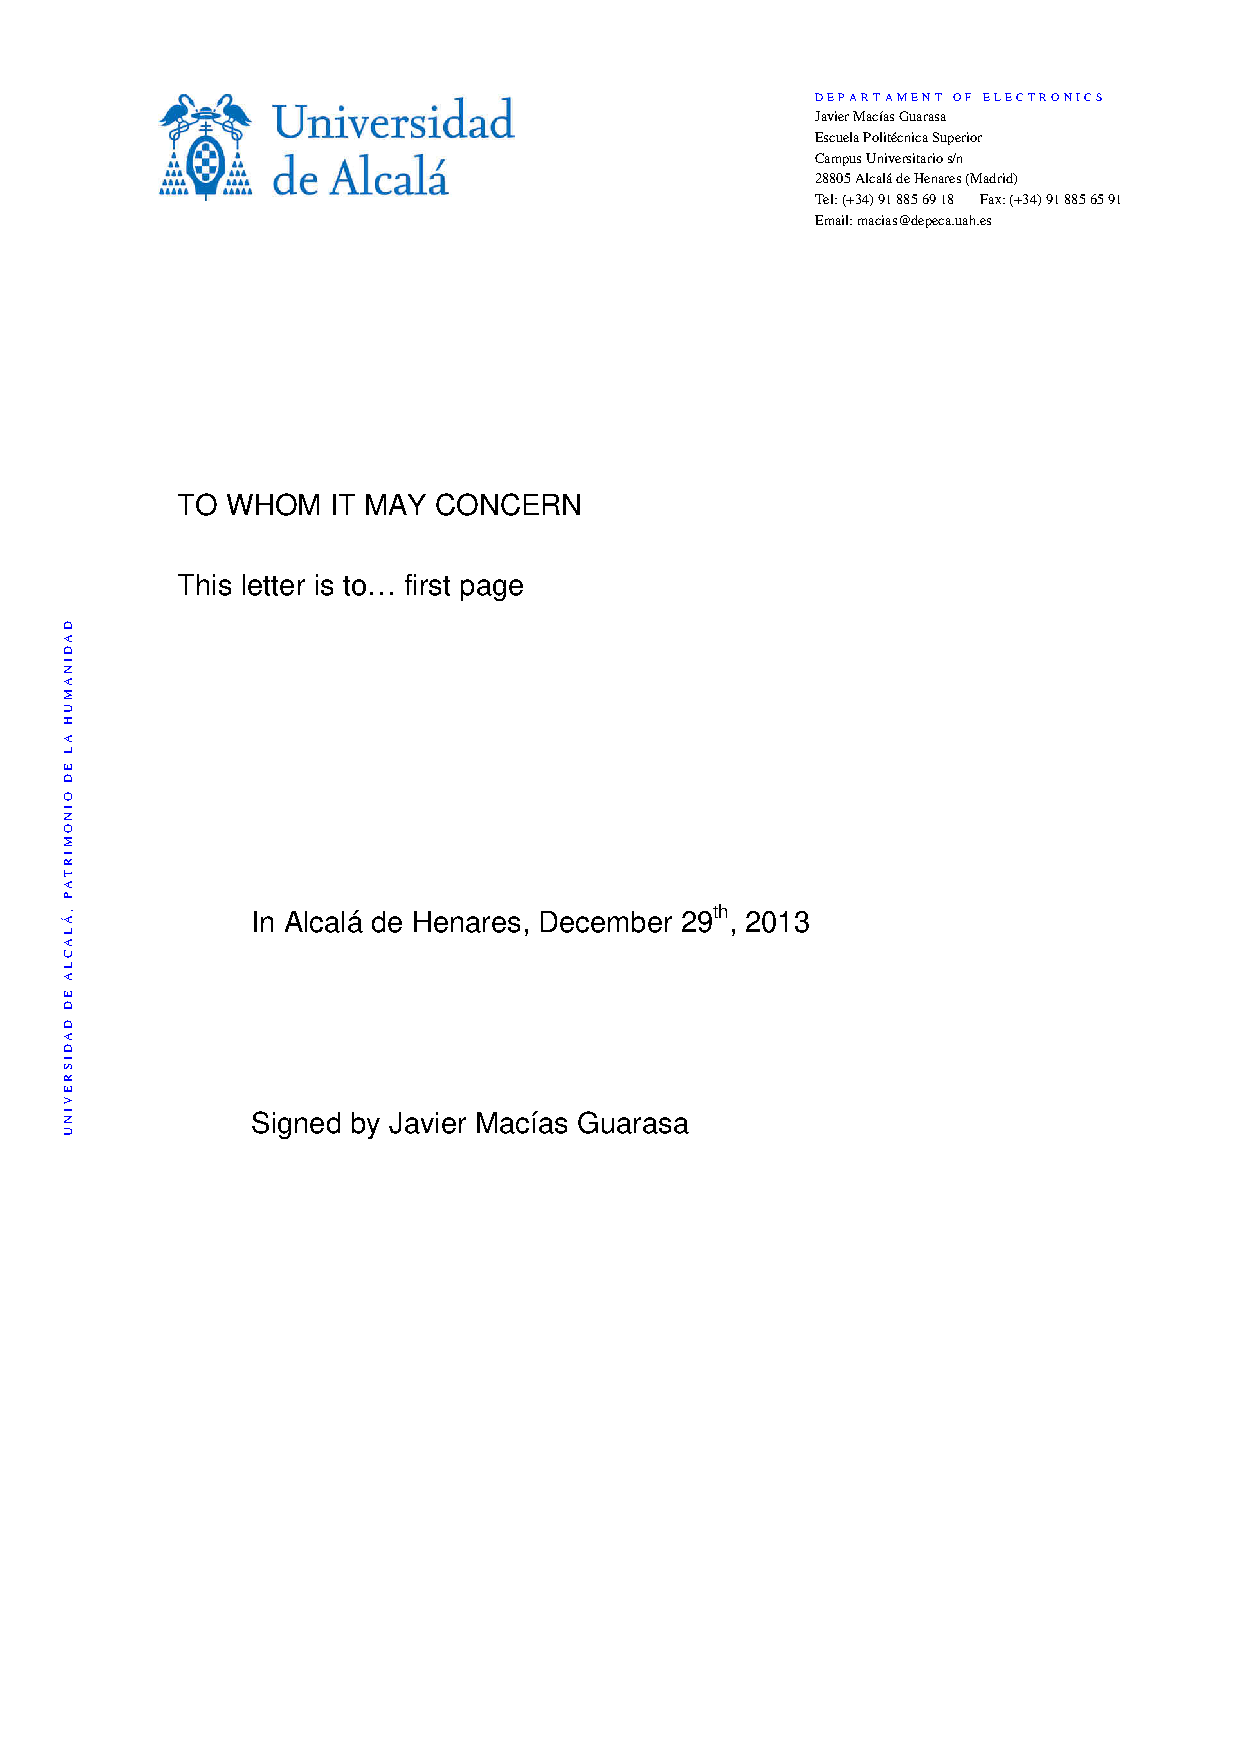
\includepdf[pages=-]{letters/sampleLetter-pages.pdf}   % include all pages of
%                                                 % pdf file

%\includepdf[pages=-]{papeleo/vistoBuenoTutorTFM-MUSEA.pdf}   % for TFMs
%\clearemptydoublepage % You need to add this after including each pdf

% Dedication+acknowledgements (dedicatorias+agradecimientos)
\ifthenelse{\equal{\myIncludeDedication}{true}}
  {%%%%%%%%%%%%%%%%%%%%%%%%%%%%%%%%%%%%%%%%%%%%%%%%%%%%%%%%%%%%%%%%%%%%%%%%%%%
% Función: dedicatoria.
%
% Uso: modifica este fichero para sustituir el ejemplo por tu contenido.
%%%%%%%%%%%%%%%%%%%%%%%%%%%%%%%%%%%%%%%%%%%%%%%%%%%%%%%%%%%%%%%%%%%%%%%%%%%

% 
% This is also courtesy of Roberto Barra
% 
% To center text in a page:
% \topskip0pt
% \vspace*{\fill}
% text
% \vspace*{\fill}

\thispagestyle{empty}

\begin{flushright}

  \topskip0pt
  \vspace*{\fill}

  \textbf{A nuestros alumnos pasados, presentes y futuros\ldots}\\

  \vspace{3cm}

  \emph{``Empieza haciendo lo necesario, luego haz lo posible y de
    pronto empezarás a hacer lo imposible.''}\\ Francisco de Asís

\end{flushright}  

\vspace{4cm}
\vspace*{\fill}

% \clearemptydoublepage



%%% Local Variables:
%%% TeX-master: "../book"
%%% End:
}
  {}
\ifthenelse{\equal{\myIncludeAcknowledgements}{true}}
  {%%%%%%%%%%%%%%%%%%%%%%%%%%%%%%%%%%%%%%%%%%%%%%%%%%%%%%%%%%%%%%%%%%%%%%%%%%%
% Función: agradecimientos.
%
% Uso: modifica este fichero para sustituir el ejemplo por tu contenido.
%%%%%%%%%%%%%%%%%%%%%%%%%%%%%%%%%%%%%%%%%%%%%%%%%%%%%%%%%%%%%%%%%%%%%%%%%%%

% Use this if you don't like the fancy style
\thispagestyle{empty}

\ifthenelse{\equal{\myLanguage}{english}}
{
  \chapter*{Acknowledgements}
  \label{cha:acknowledgements}
  \markboth{Acknowledgements}{Acknowledgements}
  \addcontentsline{toc}{chapter}{Acknowledgements}
}
{
  \chapter*{Agradecimientos}
  \label{cha:agradecimientos}
  \markboth{Agradecimientos}{Agradecimientos}
  \addcontentsline{toc}{chapter}{Agradecimientos}
}

\begin{FraseCelebre}
  \begin{Frase}
    A todos los que la presente vieren y entendieren.
  \end{Frase}
  \begin{Fuente}
    Inicio de las Leyes Orgánicas. Juan Carlos I
  \end{Fuente}
\end{FraseCelebre}

% ``Más vale un minuto de ilusión que mil horas de
% razonamiento''... (cortesía de Roberto Barra)


Este trabajo es el fruto de muchas horas de trabajo, tanto de los autores últimos de los ficheros de la distribución como de todos los que en mayor o menor medida han participado en él a lo largo de su proceso de gestación.

Mención especial merece Manuel Ocaña, el autor de la primera versión de las plantillas de proyectos fin de carrera y tesis doctorales usadas en el Departamento de Electrónica de la Universidad de Alcalá, con contribuciones de Jesús Nuevo, Pedro Revenga, Fernando Herránz y Noelia Hernández.

En la versión actual, la mayor parte de las definiciones de estilos de partida proceden de la tesis doctoral de Roberto Barra-Chicote, con lo que gracias muy especiales para él.

Añado igualmente a Gonzalo Corral de forma destacada en esta sección por ser el primero que hizo un PR sobre el repositorio github de la plantilla, y que nos llevó del arcaico ISO-8859 de bibtex a la normalidad del UTF-8 de biber (que ya hacía falta).

También damos las gracias a \input{additionalContributors.txt}, que nos han proporcionado secciones completas y/o ejemplos variados de sus tesis o proyectos/trabajos fin de carrera/grado.

Finalmente, hay incontables contribuyentes a esta plantilla, muchos de ellos encontrados gracias a la magia del buscador de Google. Hemos intentado referenciar los más importantes en los fuentes de la plantilla, aunque seguro que hemos omitido alguno. Desde aquí les damos las gracias a todos ellos por compartir su saber y buen hacer con el mundo.

En las últimas revisiones (desde principios de 2025) también cuento con la hechicería de ChatGPT y Codex, dos ayudantes incansables que me han ayudado a reorganizar la documentación, proponer redacciones, localizar incoherencias y revisar los cambios en los fuentes. Las decisiones finales y, por supuesto, los errores que queden, son responsabilidad exclusivamente mía.


% Back to normal JIC. Use it if you set \pagestyle{myplain} above
%\pagestyle{fancy}

%%% Local Variables:
%%% TeX-master: "../book"
%%% End:


}
  {}

% If this is the case, include definitions of acronyms (it's
% included before resumen.tex and abstract.tex in case you want
% to use them here
%%%%%%%%%%%%%%%%%%%%%%%%%%%%%%%%%%%%%%%%%%%%%%%%%%%%%%%%%%%%%%%%%%%%%%%%%%%
% Función: definición de los acrónimos del documento.
%
% Uso: modifica este fichero para incluir las definiciones de tu trabajo.
%%%%%%%%%%%%%%%%%%%%%%%%%%%%%%%%%%%%%%%%%%%%%%%%%%%%%%%%%%%%%%%%%%%%%%%%%%%

% This file shows some examples for glossary terms

%%%%%%%%%%%%%%%%%%%%%%%%%%%%%%%%%%%%%%%%%%%%%%%%%%%%%%%%%%%%%%%%%%%%%%%%%%%
% BEGIN example of glossary terms definition
%
\newacronym{HMI}{HMI}{Human-Machine Interfaces}
\newacronym{ETTS}{ETTS}{Emotional Text To Speech}
\newacronym{TTS}{TTS}{Text To Speech}
\newacronym{PSOLA}{PSOLA}{Pitch Synchronous OverLap Add}
\newacronym{TDPSOLA}{TD-PSOLA}{Time Domain Pitch Synchronous OverLap Add}
\newacronym{AI}{AI}{Artificial Intelligenge}

\newacronym{SPSS}{SPSS}{Statistical Parametric Speech Synthesis}
\newacronym{VC}{VC}{Voice Conversion}
\newacronym{US}{US}{Unit Selection}
\newacronym{HMM}{HMM}{Hidden Markov Model}
\newacronym{LSP}{LSP}{Line Spectral Pairs}
\newacronym{LPC}{LPC}{Linear Prediction Coefficiens}
\newacronym{LSF}{LSF}{Line Spectral Frequencies}
\newacronym{F0}{F0}{Fundamental Frequency}
\newacronym{MCEP}{MCEP}{Mel Cepstral Coefficients}
\newacronym{MGCEP}{MGCEP}{Mel Generalized Cepstral Coefficients}
\newacronym{MFCC}{MFCC}{Mel Frequency Cepstrum Coefficients}
\newacronym{ASR}{ASR}{Automatic Speech Recognition}
\newacronym{MDL}{MDL}{Minimum Description Length Criterion}
\newacronym{MSD}{MSD}{Multi Space Probability Distributions}
\newacronym{HSMM}{HSMM}{Hidden Semi-Markov Models}
\newacronym{ML}{ML}{Maximum Likelihood}
\newacronym{MLSA}{MLSA}{Mel Log Spectrum Approximation}
\newacronym{MAP}{MAP}{Maximum A Posteriori} 
\newacronym{MLLR}{MLLR}{Maximum Likelihood Linear Regression}
\newacronym{CSMAPLR}{CSMAPLR}{Constrain Structural MAP Linear Regression}
\newacronym{AV}{AV}{Average Voice}

\newacronym{ANN}{ANN}{Artificial Neural Network}

\newacronym{NIST}{NIST}{National Institute of Technology}
\newacronym{SES}{SES}{Spanish Expressive Speech}
\newacronym{EMODB}{EMODB}{Berlin Database of Emotional Speech}

\newacronym{FAUAIBO}{FAU-AIBO}{FAU AIBO Emotion Corpus}

\newacronym{SEV}{SEV}{Spanish Expressive Voices}
\newacronym{AER}{AER}{Automatic Emotion Recognition}
\newacronym{UBEC}{UBEC}{Universal Background Emotion Codebook}

\newacronym{STRAIGHT}{STRAIGHT}{Speech Transformation and Representation using Adaptive Interpolation of weiGHTed spectrum}


\newacronym{DBN}{DBN}{Dynamic Bayesian Network}
\newacronym{SQ}{SQ}{Speech Quality}
\newacronym{EIR}{EIR}{Emotion Identification Rate}
\newacronym{SIR}{SIR}{Speaker Identification Rate}
\newacronym{ES}{ES}{Emotional Strength}

\newacronym{ACCCHARS}{ÁÉÍÓÚÜÑáéíóúüñ}{Long ÁÉÍÓÚÜÑáéíóúüñ}

% In the future version of texlive, we will be able to use longplural
% and shortplural. Right now we must use \newglossaryentry.
%\newacronym[longplural={Systems on a Chip},shortplural={SOCs}]{SOC}{SOC}{System on a Chip}
\newglossaryentry{SOC}{type=\acronymtype,
        name={SOC},
        symbol={},
        sort=soc,
        plural={SOCs},
        firstplural={Systems on a Chip (SOCs)},
        description={System on a Chip},
        descriptionplural={Systems on a Chip}}

%
% END example of glossary terms definition
%%%%%%%%%%%%%%%%%%%%%%%%%%%%%%%%%%%%%%%%%%%%%%%%%%%%%%%%%%%%%%%%%%%%%%%%%%%


%%% Local Variables:
%%% TeX-master: "../book"
%%% End:
            % EDIT this file to define
                                              % the acronyms you use

% If this is the case, include definitions of acronyms (it's
% included before resumen.tex and abstract.tex in case you want
% to use them there
%%%%%%%%%%%%%%%%%%%%%%%%%%%%%%%%%%%%%%%%%%%%%%%%%%%%%%%%%%%%%%%%%%%%%%%%%%%
% Función: definición de los símbolos del documento.
%
% Uso: modifica este fichero para incluir las definiciones de tu trabajo.
%%%%%%%%%%%%%%%%%%%%%%%%%%%%%%%%%%%%%%%%%%%%%%%%%%%%%%%%%%%%%%%%%%%%%%%%%%%

% These ones for the symbols glossary

%%%%%%%%%%%%%%%%%%%%%%%%%%%%%%%%%%%%%%%%%%%%%%%%%%%%%%%%%%%%%%%%%%%%%%%%%%%
% BEGIN example of symbols definition
%
\newglossaryentry{ohm}{type=symbols,
        name={\ensuremath{\Omega}},
        symbol={\ensuremath{\Omega}}, 
        sort=ohm,
        description=unit of electrical resistance}

\newglossaryentry{angstrom}{type=symbols,
        name={\AA},
        symbol={\AA},
        sort=angstrom,
        description={non-SI unit of length}}

\newglossaryentry{xdet}{type=symbols,
        name={\ensuremath{x(t)}},
        symbol={\ensuremath{x(t)}},
        sort=xdet,
        description={Audio signal}}

\newglossaryentry{xidet}{type=symbols,
        name={\ensuremath{x_i(t)}},
        symbol={\ensuremath{x_i(t)}},
        sort=xidet,
        description={Audio signal captured at microphone $i$}}

\newglossaryentry{condindep}{type=symbols,
        name={\ensuremath{\ci}},
        symbol={\ensuremath{\ci}}, 
        sort=conditionalindependence,
        description=conditional independence}

%
% END example of symbols definition
%%%%%%%%%%%%%%%%%%%%%%%%%%%%%%%%%%%%%%%%%%%%%%%%%%%%%%%%%%%%%%%%%%%%%%%%%%%

%%% Local Variables:
%%% TeX-master: "../book"
%%% End:
              % EDIT this file to define
                                              % the symbols you use

% Now include resumen and abstract
%%%%%%%%%%%%%%%%%%%%%%%%%%%%%%%%%%%%%%%%%%%%%%%%%%%%%%%%%%%%%%%%%%%%%%%%%%%
% Función: resumen en español y palabras clave.
%
% Uso: modifica este fichero para sustituir el ejemplo por tu contenido.
%%%%%%%%%%%%%%%%%%%%%%%%%%%%%%%%%%%%%%%%%%%%%%%%%%%%%%%%%%%%%%%%%%%%%%%%%%%

\chapter*{Resumen}
\label{cha:resumen}
\markboth{Resumen}{Resumen}

\addcontentsline{toc}{chapter}{Resumen}

Este documento ha sido generado con una plantilla para memorias de
trabajos fin de carrera, fin de máster, fin de grado y tesis
doctorales. Está especialmente pensado para su uso en la Universidad de
Alcalá, pero debería ser fácilmente extensible y adaptable a otros casos
de uso. En su contenido se incluyen las instrucciones generales para
usarlo, así como algunos ejemplos de elementos que pueden ser de
utilidad. Si tenéis problemas, sugerencias o comentarios sobre el mismo,
dirigidlas por favor a \contactauthor.

\textbf{Palabras clave:} \myThesisKeywords.

%%% Local Variables:
%%% TeX-master: "../book"
%%% End:


                  % EDIT this file
%%%%%%%%%%%%%%%%%%%%%%%%%%%%%%%%%%%%%%%%%%%%%%%%%%%%%%%%%%%%%%%%%%%%%%%%%%%
% Purpose: English abstract and keywords.
%
% Usage: edit this file to replace the sample abstract with your own.
%%%%%%%%%%%%%%%%%%%%%%%%%%%%%%%%%%%%%%%%%%%%%%%%%%%%%%%%%%%%%%%%%%%%%%%%%%%

\chapter*{Abstract}
\label{cha:abstract}

\addcontentsline{toc}{chapter}{Abstract}

This document has been generated with a template for Bsc and Msc Thesis
(trabajos fin de carrera, fin de máster, fin de grado) and PhD. Thesis,
specially thought for its use in Universidad de Alcalá, although it
should be easily extended and adapted for other use cases. In its
content we include general instructions of use, and some example of
elements than can be useful. If you have problemas, suggestions or
comments on the template, please forward them to \contactauthor.


\textbf{Keywords:} \myThesisKeywordsEnglish.

%%% Local Variables:
%%% TeX-master: "../book"
%%% End:


                 % EDIT this file

% Just for TFGs/PFCs at UAH, I do nothing and leave to the author the
% inclusion of the file
%%%%%%%%%%%%%%%%%%%%%%%%%%%%%%%%%%%%%%%%%%%%%%%%%%%%%%%%%%%%%%%%%%%%%%%%%%%%
% Función: resumen extendido.
%
% Uso: modifica este fichero para sustituir el ejemplo por tu contenido.
%%%%%%%%%%%%%%%%%%%%%%%%%%%%%%%%%%%%%%%%%%%%%%%%%%%%%%%%%%%%%%%%%%%%%%%%%%%

\ifthenelse{\equal{\myLanguage}{english}}
{
\chapter*{Extended Abstract}
\label{cha:resumen-extendido}
\markboth{Extended Abstract}{Extended Abstract}

\addcontentsline{toc}{chapter}{Extended Abstract}
}
{
\chapter*{Resumen extendido}
\label{cha:resumen-extendido}
\markboth{Resumen extendido}{Resumen extendido}

\addcontentsline{toc}{chapter}{Resumen extendido}
}

Con un máximo de cuatro o cinco páginas. Se supone que sólo está
definido como obligatorio para los TFGs y PFCs de UAH.

%%% Local Variables:
%%% TeX-master: "../book"
%%% End:


       % EDIT this file

% The table of contents is always included. The remaining generated lists
% are selected independently in Config/myconfig.tex.
%%%%%%%%%%%%%%%%%%%%%%%%%%%%%%%%%%%%%%%%%%%%%%%%%%%%%%%%%%%%%%%%%%%%%%%%%%%
% Table of contents.
%%%%%%%%%%%%%%%%%%%%%%%%%%%%%%%%%%%%%%%%%%%%%%%%%%%%%%%%%%%%%%%%%%%%%%%%%%%

\clearemptydoublepage
\hypersetup{linkcolor=\mytoclinkcolor}
\tableofcontents
\hypersetup{linkcolor=\mylinkcolor}

%%% Local Variables:
%%% TeX-master: "../book"
%%% End:


\ifthenelse{\equal{\myIncludeListOfFigures}{true}}
  {%%%%%%%%%%%%%%%%%%%%%%%%%%%%%%%%%%%%%%%%%%%%%%%%%%%%%%%%%%%%%%%%%%%%%%%%%%%
% Función: índice de figuras.
%
% Uso: inclusión automática; normalmente no debes modificarlo.
% No se compila por separado.
%%%%%%%%%%%%%%%%%%%%%%%%%%%%%%%%%%%%%%%%%%%%%%%%%%%%%%%%%%%%%%%%%%%%%%%%%%%

\clearemptydoublepage
\hypersetup{linkcolor=\myloflinkcolor}
\listoffigures
\hypersetup{linkcolor=\mylinkcolor}

%%% Local Variables:
%%% TeX-master: "../book"
%%% End:
}
  {}

\ifthenelse{\equal{\myIncludeListOfTables}{true}}
  {%%%%%%%%%%%%%%%%%%%%%%%%%%%%%%%%%%%%%%%%%%%%%%%%%%%%%%%%%%%%%%%%%%%%%%%%%%%
% Función: índice de tablas.
%
% Uso: inclusión automática; normalmente no debes modificarlo.
% No se compila por separado.
%%%%%%%%%%%%%%%%%%%%%%%%%%%%%%%%%%%%%%%%%%%%%%%%%%%%%%%%%%%%%%%%%%%%%%%%%%%

\clearemptydoublepage
\hypersetup{linkcolor=\mylotlinkcolor}
\listoftables
\hypersetup{linkcolor=\mylinkcolor}

%%% Local Variables:
%%% TeX-master: "../book"
%%% End:
}
  {}

\ifthenelse{\equal{\myIncludeListOfCode}{true}}
  {%%%%%%%%%%%%%%%%%%%%%%%%%%%%%%%%%%%%%%%%%%%%%%%%%%%%%%%%%%%%%%%%%%%%%%%%%%%
% List of source code listings.
%%%%%%%%%%%%%%%%%%%%%%%%%%%%%%%%%%%%%%%%%%%%%%%%%%%%%%%%%%%%%%%%%%%%%%%%%%%

\hypersetup{linkcolor=\myothertoclinkcolor}
\ifthenelse{\equal{\myLanguage}{english}}
{
  \listof{codefloat}{List of source code listings}
  \addcontentsline{toc}{chapter}{List of source code listings}
}
{
  \listof{codefloat}{Índice de listados de código fuente}
  \addcontentsline{toc}{chapter}{Índice de listados de código fuente}
}
\hypersetup{linkcolor=\mylinkcolor}

%%% Local Variables:
%%% TeX-master: "../book"
%%% End:
}
  {}

\ifthenelse{\equal{\myIncludeListOfAlgorithms}{true}}
  {%%%%%%%%%%%%%%%%%%%%%%%%%%%%%%%%%%%%%%%%%%%%%%%%%%%%%%%%%%%%%%%%%%%%%%%%%%%
% List of algorithms.
%%%%%%%%%%%%%%%%%%%%%%%%%%%%%%%%%%%%%%%%%%%%%%%%%%%%%%%%%%%%%%%%%%%%%%%%%%%

\hypersetup{linkcolor=\myothertoclinkcolor}
\ifthenelse{\equal{\myLanguage}{english}}
{
  \renewcommand*{\algorithmcfname}{Algorithm}
  \renewcommand{\listofalgorithms}{\begingroup
    \tocfile{List of Algorithms}{loa}
    \endgroup}
}
{
  \renewcommand*{\algorithmcfname}{Algoritmo}
  \renewcommand{\listofalgorithms}{\begingroup
    \tocfile{Índice de algoritmos}{loa}
    \endgroup}
}
\listofalgorithms
\clearemptydoublepage
\hypersetup{linkcolor=\mylinkcolor}

%%% Local Variables:
%%% TeX-master: "../book"
%%% End:
}
  {}

\ifthenelse{\equal{\myIncludeListOfVideos}{true}}
  {%%%%%%%%%%%%%%%%%%%%%%%%%%%%%%%%%%%%%%%%%%%%%%%%%%%%%%%%%%%%%%%%%%%%%%%%%%%
% Función: listado de vídeos.
%
% Uso: inclusión automática; normalmente no debes modificarlo.
% No se compila por separado.
%%%%%%%%%%%%%%%%%%%%%%%%%%%%%%%%%%%%%%%%%%%%%%%%%%%%%%%%%%%%%%%%%%%%%%%%%%%

\hypersetup{linkcolor=\myothertoclinkcolor}
\ifthenelse{\equal{\myLanguage}{english}}
{
  \listofvideos
  \addcontentsline{toc}{chapter}{List of videos}
}
{
  \listofvideos
  \addcontentsline{toc}{chapter}{Índice de vídeos}
}
\hypersetup{linkcolor=\mylinkcolor}

%%% Local Variables:
%%% TeX-master: "../book"
%%% End:
}
  {}

% Now include list of acronyms and options (if this is the case)
\ifthenelse{\equal{\myIncludeListOfAcronyms}{true}}
  {%%%%%%%%%%%%%%%%%%%%%%%%%%%%%%%%%%%%%%%%%%%%%%%%%%%%%%%%%%%%%%%%%%%%%%%%%%%
% Función: listado de acrónimos.
%
% Uso: inclusión automática; normalmente no debes modificarlo.
% No se compila por separado.
%%%%%%%%%%%%%%%%%%%%%%%%%%%%%%%%%%%%%%%%%%%%%%%%%%%%%%%%%%%%%%%%%%%%%%%%%%%

% You can change the way the entries appear the first time they are
% used. I've used italics by default. I found a problem if using this:
% LaTeX adds an extra space after the acronym, so I'm commenting it out
% (if you find a solution, please let me know)
%\defglsdisplayfirst[\acronymtype]{\textit{#1}} % EDIT this if required

% This may lead to problems... I don't know how to fix it in case the
% column for acronym is wider than 0.3\linewidth
\setlength{\glsdescwidth}{0.7\linewidth}       % EDIT this if required

% Set language specific definitions...
\begin{thesislisttitlestyle}
\ifthenelse{\equal{\myLanguage}{english}}
{
\printglossary[type=\acronymtype,style=long,nonumberlist=true,title=List of Acronyms,toctitle=List of Acronyms]
\addcontentsline{toc}{chapter}{List of Acronyms}
}
{
\printglossary[type=\acronymtype,style=long,nonumberlist=true,title=Lista de acrónimos,toctitle=Lista de acrónimos]
\addcontentsline{toc}{chapter}{Lista de acrónimos}
}
\end{thesislisttitlestyle}


%%% Local Variables:
%%% TeX-master: "../book"
%%% End:

}
  {}

% Now include symbols of symbols and options (if this is the case)
\ifthenelse{\equal{\myIncludeListOfSymbols}{true}}
  {%%%%%%%%%%%%%%%%%%%%%%%%%%%%%%%%%%%%%%%%%%%%%%%%%%%%%%%%%%%%%%%%%%%%%%%%%%%
% Función: listado de símbolos.
%
% Uso: inclusión automática; normalmente no debes modificarlo.
% No se compila por separado.
%%%%%%%%%%%%%%%%%%%%%%%%%%%%%%%%%%%%%%%%%%%%%%%%%%%%%%%%%%%%%%%%%%%%%%%%%%%

% Set language specific definitions...
\begin{thesislisttitlestyle}
\ifthenelse{\equal{\myLanguage}{english}}
{
  \printglossary[type=symbols,style=long,nonumberlist=true,title=List of Symbols,toctitle=List of Symbols]
  \addcontentsline{toc}{chapter}{List of Symbols}
}
{
  \printglossary[type=symbols,style=long,nonumberlist=true,title=Lista de símbolos,title=Lista de símbolos,toctitle=Lista de símbolos]
  \addcontentsline{toc}{chapter}{Lista de símbolos}
}
\end{thesislisttitlestyle}


%%% Local Variables:
%%% TeX-master: "../book"
%%% End:
}
  {}

%
% END within-document configuration, frontpage and cover pages generation
%%%%%%%%%%%%%%%%%%%%%%%%%%%%%%%%%%%%%%%%%%%%%%%%%%%%%%%%%%%%%%%%%%%%%%%%%%%


%%%%%%%%%%%%%%%%%%%%%%%%%%%%%%%%%%%%%%%%%%%%%%%%%%%%%%%%%%%%%%%%%%%%%%%%%%%
% Now start text and numbering for mainmatter (chapter+appendices)
%%%%%%%%%%%%%%%%%%%%%%%%%%%%%%%%%%%%%%%%%%%%%%%%%%%%%%%%%%%%%%%%%%%%%%%%%%%
\mainmatter                                       % DO NOT TOUCH THIS LINE!
%\deactivatetilden                                % I removed this as it
                                                  % breaks compilation with
                                                  % TeXLive 2025 (still
                                                  % don't know why)


%%%%%%%%%%%%%%%%%%%%%%%%%%%%%%%%%%%%%%%%%%%%%%%%%%%%%%%%%%%%%%%%%%%%%%%%%%%
%%%%%%%%%%%%%%%%%%%%%%%%%%%%%%%%%%%%%%%%%%%%%%%%%%%%%%%%%%%%%%%%%%%%%%%%%%%
%%%%%%%%%%%%%%%%%%%%%%%%%%%%%%%%%%%%%%%%%%%%%%%%%%%%%%%%%%%%%%%%%%%%%%%%%%%
%%%%%%%%%%%%%%%%%%%%%%%%%%%%%%%%%%%%%%%%%%%%%%%%%%%%%%%%%%%%%%%%%%%%%%%%%%%
%%%%%%%%%%%%%%%%%%%%%%%%%%%%%%%%%%%%%%%%%%%%%%%%%%%%%%%%%%%%%%%%%%%%%%%%%%%
%%%%%%%%%%%%%%%%%%%%%%%%%%%%%%%%%%%%%%%%%%%%%%%%%%%%%%%%%%%%%%%%%%%%%%%%%%%
%%%%%%%%%%%%%%%%%%%%%%%%%%%%%%%%%%%%%%%%%%%%%%%%%%%%%%%%%%%%%%%%%%%%%%%%%%%
% Select the body configured in Config/myconfig.tex.
\ifstandarddocument
  % This is the structure used by almost every document.
  %%%%%%%%%%%%%%%%%%%%%%%%%%%%%%%%%%%%%%%%%%%%%%%%%%%%%%%%%%%%%%%%%%%%%%%%%%%
% Main content organization for standard documents.
%
% Most users should edit this file to add, remove or reorder chapters and
% appendices. Book/book.tex is the stable entry point and normally does not
% need to be modified.
%%%%%%%%%%%%%%%%%%%%%%%%%%%%%%%%%%%%%%%%%%%%%%%%%%%%%%%%%%%%%%%%%%%%%%%%%%%

%%%%%%%%%%%%%%%%%%%%%%%%%%%%%%%%%%%%%%%%%%%%%%%%%%%%%%%%%%%%%%%%%%%%%%%%%%% 
% 
% Generic template for TFC/TFM/TFG/Tesis
% 
% By:
%  + Javier Macías-Guarasa.
%    Departamento de Electrónica
%    Universidad de Alcalá
%  + Roberto Barra-Chicote.
%    Departamento de Ingeniería Electrónica
%    Universidad Politécnica de Madrid
% 
% By: + Javier Macías-Guarasa. Departamento de Electrónica Universidad de Alcalá + Roberto Barra-Chicote. Departamento de Ingeniería Electrónica Universidad Politécnica de Madrid
% 
% Based on original sources by Roberto Barra, Manuel Ocaña, Jesús Nuevo, Pedro Revenga, Fernando Herránz and Noelia Hernández. Thanks a lot to all of them, and to the many anonymous contributors found (thanks to google) that provided help in setting all this up.
% 
% See also the additionalContributors.txt file to check the name of additional contributors to this work.
% 
% If you think you can add pieces of relevant/useful examples, improvements, please contact us at (macias@depeca.uah.es)
% 
% You can freely use this template and please contribute with comments or suggestions!!!
% 
%%%%%%%%%%%%%%%%%%%%%%%%%%%%%%%%%%%%%%%%%%%%%%%%%%%%%%%%%%%%%%%%%%%%%%%%%%% 

\chapter{Introducción}
\label{cha:introduccion}

\begin{FraseCelebre}
  \begin{Frase}
    Desocupado lector, sin juramento me podrás creer que quisiera que este libro [...] fuera el más hermoso, el más gallardo y más discreto que pudiera imaginarse\footnote{Tomado de ejemplos del proyecto \texis{}.}.
  \end{Frase}
  \begin{Fuente}
    Miguel de Cervantes, Don Quijote de la Mancha
  \end{Fuente}
\end{FraseCelebre}


\section{Presentación}
\label{sec:presentacion}

Esta plantilla\footnote{Asegúrate de compilar de nuevo el documento, como se explica en la sección~\ref{sec:compilacion}, para verificar que todo funciona y por si se ha producido algún cambio en los fuentes que todavía no esté reflejado en los PDF de ejemplo precompilados.} proporciona una estructura común para redactar trabajos académicos con \LaTeX{}. Incluye soporte para trabajos fin de carrera de planes anteriores, trabajos fin de grado, trabajos fin de máster y tesis doctorales. La mayor parte de las portadas y documentos administrativos están adaptados a titulaciones de la Universidad de Alcalá, aunque también conservamos soporte para determinados programas de doctorado de la Universidad Politécnica de Madrid\footnote{En la UPM se incluye actualmente soporte para tesis de la Escuela Técnica Superior de Ingenieros de Telecomunicación. La extensión a otros tipos de trabajo sería posible, pero todavía no está incorporada a la plantilla.}.

Además del libro principal, hemos incluido una plantilla para preparar el anteproyecto, descrita en la sección~\ref{sec:plantilla-de-anteproyecto}, y distintos documentos administrativos relacionados con la presentación, el depósito, la evaluación y la publicación de los trabajos, que se detallan en la sección~\ref{sec:introapp1}. Todos ellos comparten la configuración del trabajo, del autor y de los tutores, para que no tengas que introducir los mismos datos una y otra vez.

También hemos preparado capítulos y apéndices de ejemplo con secciones de carácter tutorial. En ellas intentamos explicar algunas de las posibilidades de la plantilla y mostrar elementos habituales que pueden resultar útiles, aunque no pretendemos que este documento sustituya a una guía completa de \LaTeX{}.

Nuestro objetivo es facilitar tanto la composición del documento como el cumplimiento de los formatos institucionales. Aun así, estos formatos pueden cambiar con el tiempo, por lo que te recomendamos comprobar siempre la normativa vigente de tu titulación antes de entregar la documentación.

\section{Organización del repositorio}
\label{sec:organizacion-repositorio}

Los principales directorios del repositorio son:

\begin{itemize}
  \item \texttt{Book/}: documento académico principal, incluidas las cubiertas, capítulos, anexos, bibliografía, resúmenes y demás elementos del libro.
  \item \texttt{Config/}: configuración compartida, selección de la titulación y datos personales y académicos definidos en \texttt{myconfig.tex}.
  \item \texttt{Anteproyecto/}: plantilla para preparar la propuesta o anteproyecto del trabajo.
  \item \texttt{PapeleoTFG/}: formularios administrativos relacionados con los trabajos fin de grado.
  \item \texttt{PapeleoTFM/}: formularios administrativos relacionados con los trabajos fin de máster.
  \item \texttt{PapeleoPHD/}: formularios administrativos relacionados con las tesis doctorales.
\end{itemize}

El repositorio Git completo contiene además \texttt{AdminScripts/}, \texttt{Deprecated/}, \texttt{normativas/}, \texttt{UsefulDocs/} y documentos Markdown destinados al mantenimiento, la consulta histórica y la preparación de versiones. Estos elementos no se incluyen en la distribución ZIP/TGZ ordinaria porque no son necesarios para utilizar la plantilla.

El fichero \texttt{sync-git-sources.sh} situado en la raíz implementa la sincronización opcional y basada en dependencias que puedes solicitar mediante \texttt{make sync-git-sources}. Normalmente utilizarás el objetivo del \texttt{Makefile} y no ejecutarás directamente este script.

La configuración general se realiza en \texttt{Config/myconfig.tex}, como se explica en la sección~\ref{sec:definicion-del-tipo}. Los distintos documentos del repositorio leen este archivo para mantener coherentes los nombres, títulos, fechas y demás datos compartidos.



\section{Cómo utilizar esta guía}
\label{sec:itinerario-guia}

Si es la primera vez que utilizas la plantilla, te recomendamos comenzar por el capítulo~\ref{cha:primeros-pasos}: allí explicamos qué necesitas y cómo generar el primer PDF sin obligarte a trabajar desde una terminal. Después puedes completar los datos de tu trabajo con la referencia del capítulo~\ref{cha:configuracion}, consultar en el capítulo~\ref{cha:estructura-documento} qué partes del documento debes editar y cuáles puedes dejar tal como están, y descubrir en el capítulo~\ref{cha:elementos-utilidad} los recursos que hemos incorporado como parte de la plantilla.

Los documentos complementarios se describen en el capítulo~\ref{cha:documentos-complementarios}. Hemos reservado el capítulo~\ref{cha:compilacion-avanzada} para el \texttt{Makefile}, el control de cambios y otras herramientas que no necesitas para comenzar. Finalmente, los capítulos~\ref{cha:elementos-basicos} y~\ref{cha:ejemplos-avanzados} reúnen ejemplos de \LaTeX{} que puedes consultar cuando quieras incorporar esos recursos a tu propio trabajo.

No esperamos que leas toda la guía antes de empezar ni que utilices todas las posibilidades de la plantilla. Queremos que puedas avanzar poco a poco y volver a cada capítulo cuando realmente lo necesites.

%%% Local Variables:
%%% TeX-master: "../book"
%%% End:

%%%%%%%%%%%%%%%%%%%%%%%%%%%%%%%%%%%%%%%%%%%%%%%%%%%%%%%%%%%%%%%%%%%%%%%%%%%
% Función: primeros pasos con la plantilla.
%
% Uso: modifica este fichero para adaptar el contenido a tu trabajo.
%%%%%%%%%%%%%%%%%%%%%%%%%%%%%%%%%%%%%%%%%%%%%%%%%%%%%%%%%%%%%%%%%%%%%%%%%%%

\chapter{Primeros pasos}
\label{cha:primeros-pasos}

En este capítulo te acompañamos desde la descarga de la plantilla hasta la generación del primer PDF. Primero presentaremos los archivos publicados y los documentos de ejemplo, después revisaremos los requisitos y explicaremos cómo configurar la compilación en GNU/Linux, Windows, macOS y Overleaf, a continuación presentaremos brevemente la plantilla de anteproyecto y, por último, explicaremos cómo preparar una estructura mínima para comenzar a escribir tu trabajo y cómo registrar correctamente sus fuentes en Git. Para empezar no necesitas conocer el \texttt{Makefile} ni utilizar una terminal: puedes trabajar con tu editor habitual de \LaTeX{}.

\section{Descarga y documentos de ejemplo}
\label{sec:descarga-ejemplos}

La \href{https://www.dropbox.com/sh/mm6fwh3ruuuyjz2/AABDUmo7Xj1S968FeJgbmFPva?dl=0}{carpeta de descargas de la plantilla} contiene los archivos ZIP y TGZ de la versión publicada y una selección reducida de documentos completos. Te recomendamos comenzar por \texttt{TFG-GIEC-spanish.pdf}, que utiliza la estructura y el estilo predeterminados. El fichero \texttt{01-DOWNLOAD-GUIDE.pdf}, situado al principio de la carpeta, enumera todos los ejemplos disponibles y explica qué idioma, estructura, estilo tipográfico, política de fuentes institucionales y cubierta muestra cada uno.

Los PDF precompilados son ejemplos representativos y no una copia para cada titulación admitida. Si no encuentras un documento dedicado a tu grado o máster, no significa que no esté soportado: consulta los identificadores disponibles en \texttt{Config/myconfig.tex} y la lista descrita en el capítulo~\ref{cha:configuracion}. El fichero \texttt{RELEASE.txt} de la carpeta te permite comprobar a qué versión corresponden los archivos publicados.

\section{Prerrequisitos}
\label{sec:prerrequisitos}

Si trabajas localmente, para compilar la plantilla necesitas una distribución de \LaTeX{} suficientemente completa y actualizada. TeX Live es una opción habitual en GNU/Linux, MiKTeX y TeX Live están disponibles para Windows, y MacTeX proporciona una distribución adaptada a macOS. Asegúrate de que la distribución que elijas proporcione \texttt{pdflatex} y Biber, además de los paquetes cargados desde \texttt{Config/preamble.tex}.

Si prefieres trabajar en línea con Overleaf, no necesitas instalar una distribución ni un editor en tu equipo. La plataforma proporciona el entorno de compilación; en la sección~\ref{sec:compilacion-overleaf} te explicamos cómo importar la plantilla y seleccionar el documento principal.

Biber es necesario cuando el documento incluye bibliografía. Si utilizas acrónimos o símbolos, también necesitarás \texttt{makeglossaries}; el libro de ejemplo distribuido con la plantilla contiene ambos elementos y, por tanto, requiere esta herramienta para generar todos sus listados.

Si durante la compilación recibes un aviso de que falta un fichero \texttt{.sty}, instala el paquete de tu distribución de \LaTeX{} que lo contiene. En MiKTeX puedes activar la instalación automática de paquetes; TeX Live y MacTeX proporcionan sus propias herramientas para administrar los paquetes instalados.

No necesitas utilizar \texttt{make} para trabajar con la plantilla. Puedes compilarla con cualquier editor o herramienta de construcción de \LaTeX{} que permita configurar las herramientas descritas en la sección~\ref{sec:compilacion}; si lo prefieres, también puedes hacerlo desde una terminal. El \texttt{Makefile} incluido es únicamente una forma opcional de automatizar el proceso y resulta especialmente cómodo en sistemas GNU/Linux.


\section{Compilación del documento principal}
\label{sec:compilacion}

Antes de compilar el documento, completa la configuración compartida en \texttt{Config/myconfig.tex} siguiendo las indicaciones de la sección~\ref{sec:definicion-del-tipo}. Después, abre \texttt{Book/book.tex} como documento principal en tu editor de \LaTeX{} y utiliza su función habitual de compilación o construcción.

Para generar correctamente todos los elementos del libro, configura el editor para utilizar \texttt{pdflatex} como compilador y Biber como procesador de la bibliografía. Si utilizas acrónimos o símbolos, añade también \texttt{makeglossaries} a la cadena de construcción. Finalmente, realiza las pasadas adicionales de \texttt{pdflatex} necesarias para actualizar las referencias cruzadas, los índices, la bibliografía y los glosarios.

\subsection{GNU/Linux}

En GNU/Linux puedes utilizar tu editor de \LaTeX{} preferido. Asegúrate de abrir \texttt{Book/book.tex} como documento principal y de configurar la cadena de construcción como se explica en la sección~\ref{sec:compilacion}.

Si prefieres automatizar el proceso mediante \texttt{make}, consulta \textit{Compilación mediante el \texttt{Makefile}} (apartado~\ref{sec:compilacion-makefile}), donde se describen el procedimiento y los objetivos disponibles.

\subsection{Windows}

En Windows puedes utilizar MiKTeX o TeX Live junto con TeXstudio u otro editor de \LaTeX{}. En la configuración del editor, selecciona Biber como procesador de la bibliografía y, si utilizas acrónimos o símbolos, añade \texttt{makeglossaries} a la cadena de construcción. Para ejecutar \texttt{makeglossaries} también necesitas un intérprete de Perl; Strawberry Perl es una de las alternativas disponibles para Windows.

No necesitas instalar \texttt{make} para trabajar con la plantilla en Windows. Si quieres utilizar el \texttt{Makefile} descrito en el apartado~\ref{sec:compilacion-makefile}, puedes hacerlo desde un entorno compatible que proporcione las herramientas requeridas, como WSL, aunque normalmente te resultará más sencillo configurar la cadena de compilación en el propio editor.

Parte de estas instrucciones se basa en la información que nos proporcionó Cristina Losada sobre la configuración de TeXmaker en Windows. Muchas gracias por su ayuda.

\subsection{macOS}

En macOS puedes utilizar MacTeX junto con TeXShop, TeXstudio u otro editor compatible. Configura la cadena de construcción para incluir \texttt{pdflatex}, Biber y, si utilizas acrónimos o símbolos, \texttt{makeglossaries} en el orden explicado en la sección~\ref{sec:compilacion}.

Si tu editor no actualiza correctamente los acrónimos o símbolos, utiliza desde el propio editor la opción para ejecutar \texttt{makeglossaries} y realiza después dos nuevas pasadas de \texttt{pdflatex}. No necesitas borrar el resto de los ficheros del proyecto para regenerar los glosarios.

Las primeras comprobaciones de la generación de glosarios en macOS fueron realizadas y compartidas con nosotros por Carlos Cruz. Muchas gracias por su ayuda.

\subsection{Overleaf}
\label{sec:compilacion-overleaf}

Si no quieres instalar y mantener un entorno local, puedes trabajar en línea mediante \href{https://www.overleaf.com/}{Overleaf}. Para importar la plantilla sigue estos pasos:

\begin{itemize}
  \item Inicia sesión en Overleaf y selecciona \textit{New Project} y, a continuación, \textit{Upload Project}.
  \item Sube sin descomprimir el fichero ZIP correspondiente a tu titulación, disponible en la \href{https://www.dropbox.com/sh/mm6fwh3ruuuyjz2/AABDUmo7Xj1S968FeJgbmFPva?dl=0}{carpeta de descargas de la plantilla}.
  \item Abre las opciones del proyecto y selecciona \texttt{Book/book.tex} como \textit{Main document}.
  \item Comprueba que el compilador seleccionado sea pdfLaTeX y compila el proyecto.
\end{itemize}

Overleaf gestiona la cadena de construcción con sus propias herramientas, por lo que no necesitas ejecutar el \texttt{Makefile}. El libro utiliza Biber para la bibliografía y \texttt{makeglossaries} para los acrónimos y símbolos; después de importar el proyecto, comprueba que se generen correctamente la bibliografía y ambos listados. Si alguno no se actualiza, revisa primero el documento principal seleccionado y utiliza la opción de recompilar el proyecto desde cero.

El libro de ejemplo es relativamente complejo y su compilación puede superar el tiempo disponible en algunos planes de Overleaf. Si la compilación se interrumpe por este motivo, comprueba los límites vigentes de tu cuenta y elimina temporalmente los ejemplos o elementos opcionales que no necesites. Para generar el anteproyecto o un formulario administrativo tendrás que cambiar el documento principal, como se explica en el capítulo~\ref{cha:documentos-complementarios}.


\section{Trabajo con el anteproyecto}
\label{sec:primeros-pasos-anteproyecto}

Si antes de comenzar la memoria necesitas preparar un anteproyecto, utiliza \texttt{Anteproyecto/anteproyecto.tex} como documento principal. Esta plantilla reutiliza los datos definidos en \texttt{Config/myconfig.tex} y puedes compilarla con tu editor habitual, mediante su \texttt{Makefile} opcional o, en Overleaf, seleccionándola como \textit{Main document}. Encontrarás una descripción más completa de su contenido y compilación en la sección~\ref{sec:plantilla-de-anteproyecto}.

\section{Preparación de una estructura mínima}
\label{sec:estructura-minima}

Después de descargar la plantilla, compila directamente el fichero \texttt{Book/book.tex} antes de comenzar a modificarla. El resultado será este manual completo, que también contiene ejemplos de los elementos que puedes utilizar en tu trabajo. Esta primera compilación te permitirá comprobar que tu entorno funciona correctamente y consultar el manual mientras conoces la plantilla.

Una vez que hayas comprobado que todo funciona, puedes comenzar a escribir tu memoria a partir de la estructura mínima y casi vacía que hemos preparado. Mantén \texttt{standard} como valor de \texttt{\textbackslash{}myDocumentStructure}, utiliza \texttt{Book/content-standard.tex} para organizar tus capítulos, bibliografía y apéndices, y sigue compilando el único punto de entrada \texttt{Book/book.tex}. Antes de sustituir ningún fichero, conserva una copia de tu trabajo si ya has comenzado a modificar la plantilla.

Para preparar manualmente una memoria convencional con \texttt{standard}, sigue estos pasos:

\begin{itemize}
  \item Elimina los ficheros \texttt{.tex} situados directamente en \texttt{chapters/} y \texttt{appendix/}; no elimines sus subdirectorios ni su contenido.
  \item Copia a \texttt{chapters/} los ficheros de capítulo de \texttt{chapters/bare/}, sin copiar allí el fichero \texttt{content-standard.tex}, y copia los ficheros de \texttt{appendix/bare/} a \texttt{appendix/}.
  \item Sustituye \texttt{Book/content-standard.tex} por \texttt{Book/chapters/bare/content-standard.tex}; este fichero ya incluye los capítulos y apéndices mínimos que acabas de copiar.
  \item Revisa en \texttt{Config/myconfig.tex} las variables \texttt{\textbackslash{}myInclude...} descritas en la sección~\ref{sec:elementos-opcionales-configuracion}. Estas variables controlan la carta PDF de ejemplo, la dedicatoria, los agradecimientos y los índices independientes de figuras, tablas, acrónimos, símbolos, código, algoritmos y vídeos; deja en \texttt{false} los elementos que todavía no necesites.
\end{itemize}

Si utilizas \texttt{make}, ejecuta \texttt{make bare} desde \texttt{Book/}. Como \texttt{standard} es el valor predeterminado, el objetivo crea una copia de seguridad, instala los capítulos, apéndices y el fichero \texttt{content-standard.tex} mínimos, y desactiva el material opcional de ejemplo. También puedes solicitar explícitamente esta preparación mediante \texttt{make bare-standard}; \texttt{bare-chapters} se conserva como alias compatible. Estos objetivos se describen con más detalle en la sección~\ref{sec:compilacion-makefile}.

\subsection{Caso particular: tesis por compendio de publicaciones}

Solo si vas a preparar una tesis doctoral por compendio debes seleccionar \texttt{compendium}. En ese caso elimina los ficheros \texttt{.tex} situados directamente en \texttt{Book/chapters/compendium/}, copia allí los seis capítulos de \texttt{Book/chapters/compendium/bare/}, sin copiar el fichero \texttt{content-compendium.tex}, y utiliza este último para sustituir \texttt{Book/content-compendium.tex}. El objetivo \texttt{make bare} realiza esas operaciones automáticamente cuando detecta esa estructura. La versión completa distribuida se conserva en \texttt{Book/chapters/compendium/orig/} y puedes restaurarla mediante \texttt{make orig-compendium}. Consulta la sección~\ref{sec:tesis-compendio} para conocer la organización de las dos partes y la forma de incorporar las publicaciones.

\section{Preparación del repositorio Git}
\label{sec:preparacion-repositorio-git}

Después de comprobar la compilación y preparar la estructura mínima, te recomendamos crear un repositorio Git para tu trabajo y realizar un primer commit con los ficheros necesarios para reconstruir los documentos. Puedes prepararlo desde una aplicación gráfica sin utilizar la línea de comandos o, si dispones de \texttt{make} y Bash, dejar que la plantilla determine las dependencias compilables. En ambos casos debes revisar los cambios antes de crear el commit: \LaTeX{} genera numerosos ficheros auxiliares que no forman parte de tu trabajo y que solo añadirían ruido al historial.

\subsection{Ficheros que debes versionar}

En el primer commit debes incluir los siguientes tipos de ficheros:

\begin{itemize}
  \item Los ficheros de configuración compartida de \texttt{Config/}, en particular \texttt{myconfig.tex}, y los ficheros estructurales que cargan tus documentos.
  \item \texttt{Book/book.tex}, \texttt{Book/content-standard.tex} o, en el caso especializado, \texttt{Book/content-compendium.tex}, además de los capítulos, apéndices, resúmenes, bibliografía y demás fuentes \texttt{.tex} o \texttt{.bib} que utilice realmente el libro.
  \item \texttt{Anteproyecto/anteproyecto.tex} y los formularios de \texttt{PapeleoTFG/}, \texttt{PapeleoTFM/} o \texttt{PapeleoPHD/} que quieras poder generar.
  \item Las figuras, diagramas, logotipos, cartas y otros recursos que los documentos lean durante la compilación. Esto incluye los PDF que sean recursos de entrada, por ejemplo una carta incorporada mediante \texttt{\textbackslash{}includepdf}.
  \item Los \texttt{Makefile}, los ficheros \texttt{.gitignore}, el fichero \texttt{README.md}, la licencia y cualquier script propio que necesites para reconstruir los documentos.
\end{itemize}

A medida que avances, añade los nuevos capítulos, referencias bibliográficas, figuras, datos o scripts que incorpores al trabajo y registra también la eliminación de los que dejes de utilizar. Antes de cada commit, revisa la lista de cambios que muestra tu cliente de Git y selecciona los ficheros que correspondan; si trabajas desde la línea de comandos, puedes consultar \texttt{git status}, añadir rutas concretas mediante \texttt{git add} y retirar únicamente del índice un fichero que quieras conservar en tu equipo mediante \texttt{git rm --cached}.

No debes subir nunca los auxiliares creados durante la compilación, como los ficheros \texttt{.aux}, \texttt{.log}, \texttt{.fls}, \texttt{.fdb\_latexmk}, \texttt{.synctex.gz}, \texttt{.bcf}, \texttt{.blg}, \texttt{.bbl}, \texttt{.run.xml}, \texttt{.toc}, \texttt{.lof} o \texttt{.lot}; tampoco los archivos temporales del editor, los paquetes de distribución ni los PDF generados del libro, el anteproyecto o el papeleo. Como excepción, puedes conservar la versión final definitiva del documento si existe una razón clara para versionarla, pero no acumules en Git los PDF de cada compilación.

\subsection{Primer commit mediante una aplicación gráfica}

La forma más sencilla de preparar el primer commit sin utilizar la línea de comandos consiste en partir de la distribución oficial y conservar el fichero \texttt{.gitignore} incluido en su directorio raíz. Este fichero indica a Git qué auxiliares, resultados de compilación y ficheros temporales debe ignorar, y las aplicaciones gráficas habituales respetan esas reglas.

Puedes utilizar GitHub Desktop, el panel de control de versiones de Visual Studio Code, GitKraken, Sourcetree u otro cliente gráfico. Aunque no todos presentan las mismas opciones ni emplean los mismos nombres, todos permiten seleccionar los cambios que formarán parte de un commit. Sigue este procedimiento:

\begin{itemize}
  \item Abre como repositorio la carpeta raíz de la plantilla, en la que se encuentran \texttt{README.md}, \texttt{Config/} y \texttt{Book/}; si todavía no es un repositorio, utiliza la opción de la aplicación para crear o inicializar uno en esa carpeta.
  \item Selecciona todos los cambios no ignorados para incluirlos en el primer commit. Según la aplicación, la operación puede denominarse \emph{Stage all}, \emph{Stage all changes}, \emph{Select all} o mostrarse como una casilla que permite marcar todos los ficheros.
  \item Revisa la lista antes de confirmar. Debes reconocer las fuentes y los recursos descritos en el apartado anterior, pero no deben aparecer auxiliares de \LaTeX{} ni los PDF generados durante tus pruebas.
  \item Escribe un mensaje que describa el inicio de tu trabajo y crea el commit. Publicarlo o sincronizarlo posteriormente con GitHub, GitLab u otro servidor es una operación separada y opcional.
\end{itemize}

Este procedimiento resulta especialmente apropiado para el primer commit. En los siguientes puedes volver a seleccionar desde la aplicación los ficheros nuevos, modificados o eliminados, pero tendrás que decidir cuáles siguen siendo necesarios. No fuerces la inclusión de un fichero que Git haya ignorado sin comprobar primero por qué coincide con una regla de \texttt{.gitignore}.

\subsection{Sincronización mediante el \texttt{Makefile}}

Antes de utilizar este objetivo debes trabajar dentro de un repositorio Git, bien porque hayas clonado la plantilla desde GitHub u otro servidor, bien porque hayas creado un repositorio local en la carpeta raíz mediante \texttt{git init .}; después de preparar y confirmar el primer commit podrás configurar un repositorio remoto y publicarlo mediante \texttt{git push}.

Si dispones de \texttt{make} y Bash, ejecuta desde el directorio raíz del proyecto:

\begin{verbatim}
make sync-git-sources
\end{verbatim}

Este objetivo es la alternativa avanzada y dependiente de la compilación al procedimiento gráfico. Genera de nuevo las dependencias de \LaTeX{} del libro, el anteproyecto y todos los formularios, identifica los ficheros locales imprescindibles para compilarlos y los compara con el contenido versionado. Antes de actuar muestra los ficheros que añadirá o actualizará y aquellos que dejarán de estar versionados, y te pide confirmación. Si aceptas, actualiza únicamente el índice de Git: los ficheros descartados permanecen en el disco y no se ejecutan ni \texttt{git commit} ni \texttt{git push}. Al terminar, revisa \texttt{git status} y crea tú mismo el commit adecuado.

Puedes volver a ejecutar el objetivo cada vez que cambien las dependencias. Si no puede generarse información de dependencias, el proceso se detiene antes de modificar el índice; si una fuente produce dependencias pero no completa la compilación, muestra una advertencia para que revises el error. Como medida de seguridad, el objetivo está desactivado cuando detecta la marca local que identifica el repositorio oficial de mantenimiento de la plantilla.

\section{Resumen del capítulo}
\label{sec:resumen-primeros-pasos}

Ya sabes qué archivos encontrarás en la carpeta de descargas, qué herramientas necesita la plantilla, cómo generar el documento desde tu editor habitual en GNU/Linux, Windows o macOS, o mediante Overleaf, cómo trabajar con el anteproyecto, cómo preparar la estructura mínima con la que puedes comenzar a escribir tu trabajo y cómo registrar correctamente sus fuentes en Git. Recuerda que Biber es necesario para la bibliografía y que solo tendrás que ejecutar \texttt{makeglossaries} cuando utilices acrónimos o símbolos; el siguiente paso es adaptar las variables descritas en el capítulo~\ref{cha:configuracion}.

%%% Local Variables:
%%% TeX-master: "../book"
%%% End:

%%%%%%%%%%%%%%%%%%%%%%%%%%%%%%%%%%%%%%%%%%%%%%%%%%%%%%%%%%%%%%%%%%%%%%%%%%%
% Función: configuración del documento.
%
% Uso: modifica este fichero para adaptar el contenido a tu trabajo.
%%%%%%%%%%%%%%%%%%%%%%%%%%%%%%%%%%%%%%%%%%%%%%%%%%%%%%%%%%%%%%%%%%%%%%%%%%%

\chapter{Configuración de la plantilla}
\label{cha:configuracion}

La mayor parte de la adaptación de la plantilla se realiza en \texttt{Config/myconfig.tex}. En este capítulo describimos todas las variables disponibles para que puedas utilizarlo como referencia: comenzaremos por la configuración general y recorreremos después los datos académicos, las fechas, la publicación, los enlaces y los ajustes de compatibilidad. Normalmente solo tendrás que completar las que correspondan a tu tipo de trabajo y a los documentos que vayas a generar.

A partir de los datos que indiques, la plantilla adapta automáticamente parte de los textos generados. Entre otros aspectos, selecciona las formas correspondientes al género gramatical de la persona autora, los tutores y otros cargos, y ajusta el singular o el plural según exista únicamente un tutor o también un cotutor. De este modo, puede generar automáticamente expresiones como \emph{tutor/tutora}, \emph{director/directora}, \emph{tutor/tutores} o \emph{emite/emiten}. Esta adaptación se aplica principalmente a las cubiertas y a los documentos administrativos; revisa siempre el PDF resultante para comprobar que la redacción es adecuada para tu caso.

\section{Configuración del documento}
\label{sec:definicion-del-tipo}

La configuración compartida se encuentra en \texttt{Config/myconfig.tex}. Este fichero contiene los datos utilizados para generar el libro, el anteproyecto y los documentos administrativos, por lo que normalmente tendrás que adaptarlo antes de editar el contenido de tu trabajo. Las variables se definen mediante órdenes \texttt{\textbackslash{}newcommand}; para cambiar una variable, modifica únicamente el contenido situado entre las últimas llaves de su definición, sin alterar el nombre de la orden.

Además de completar \texttt{Config/myconfig.tex}, revisa \texttt{Book/content-standard.tex}, que determina los capítulos, la bibliografía y los apéndices de la estructura utilizada por la inmensa mayoría de los documentos. \texttt{Book/book.tex} es el punto de entrada estable para la compilación y normalmente no tendrás que modificarlo. Solo si preparas una tesis doctoral por compendio trabajarás con el fichero especializado \texttt{Book/content-compendium.tex}, descrito en la sección~\ref{sec:tesis-compendio}.

\section{Estructura, idioma, titulación y presentación de los tutores}

Las siguientes variables controlan la estructura, el idioma, la titulación y la presentación conjunta o separada de los tutores:

\begin{itemize}
  \item \texttt{\textbackslash{}myDocumentStructure}: estructura del documento principal. Mantén el valor \texttt{standard} para los TFG, TFM, tesis doctorales convencionales y el resto de documentos habituales; esta opción utiliza \texttt{Book/content-standard.tex}. El valor \texttt{compendium} queda reservado para tesis doctorales presentadas por compendio de publicaciones y utiliza \texttt{Book/content-compendium.tex}. En ambos casos debes compilar \texttt{Book/book.tex}.
  \item \texttt{\textbackslash{}myLanguage}: idioma principal del documento. Admite los valores \texttt{spanish} y \texttt{english}. Esta selección determina, entre otros elementos, los textos automáticos, las cabeceras, el título utilizado y las palabras clave incorporadas a los metadatos del PDF.
  \item \texttt{\textbackslash{}myDegree}: identificador de la titulación o del tipo concreto de documento. Su valor determina el tipo general de trabajo y selecciona automáticamente las portadas, contraportadas, nombres de titulación y otros textos aplicables.
  \item \texttt{\textbackslash{}myFlagSplittedAdvisors}: controla cómo se presentan el tutor y el cotutor en las páginas que admiten ambas formas. El valor \texttt{true} utiliza líneas separadas para el tutor y el cotutor; el valor \texttt{false} utiliza una denominación conjunta.
  \item \texttt{\textbackslash{}mySpecialty}: especialidad o itinerario asociado a la titulación. Puede dejarse vacío cuando no resulte aplicable.
\end{itemize}

Los identificadores admitidos actualmente por \texttt{\textbackslash{}myDegree}, organizados por universidad y centro, son:

\begin{itemize}
  \item \textbf{Universidad de Alcalá}:
  \begin{itemize}
    \item \textbf{Escuela Politécnica Superior}: trabajos fin de carrera \texttt{IT}, \texttt{IE}, \texttt{ITTSE}, \texttt{ITTST} e \texttt{ITI}; trabajos fin de grado \texttt{GITT}, \texttt{GIEC}, \texttt{GIT}, \texttt{GIST}, \texttt{GIC}, \texttt{GII}, \texttt{GMC}, \texttt{GIS}, \texttt{GSI}, \texttt{GISI}, \texttt{GIEAI} y \texttt{GITI}; trabajos fin de máster \texttt{MUSEA}, \texttt{MUIT}, \texttt{MUII}, \texttt{MUIE}, \texttt{MUCTE}, \texttt{MUANBD} y \texttt{MUC}; y tesis doctoral \texttt{PHDUAH}. Los identificadores de trabajos fin de carrera corresponden a titulaciones anteriores al Espacio Europeo de Educación Superior y se conservan por compatibilidad.
    \item \textbf{Facultad de Ciencias}: trabajos fin de grado \texttt{GFIE}, \texttt{GBS}, \texttt{GB}, \texttt{GQ}, \texttt{GCA} y \texttt{GCCTF}.
  \end{itemize}
  \item \textbf{Universidad Rey Juan Carlos}:
  \begin{itemize}
    \item \textbf{Escuela Superior de Ciencias Experimentales y Tecnología}: trabajo fin de grado \texttt{ITIURJC}.
  \end{itemize}
  \item \textbf{Universidad Politécnica de Madrid}:
  \begin{itemize}
    \item \textbf{Escuela Técnica Superior de Ingenieros de Telecomunicación}: tesis doctoral \texttt{PHDUPM}.
  \end{itemize}
  \item \textbf{Grupo de investigación GEINTRA}: informe de investigación \texttt{GEINTRARR}, cuyo soporte se considera todavía experimental.
\end{itemize}

Consulta siempre la lista actualizada de identificadores admitidos en los comentarios que aparecen inmediatamente antes de la definición de \texttt{\textbackslash{}myDegree} en \texttt{Config/myconfig.tex}. Solo tienes que elegir allí el identificador correspondiente; la plantilla seleccionará automáticamente los datos y las páginas institucionales aplicables.

\section{Estilos tipográficos del documento (implementación preliminar)}
\label{sec:estilos-tipograficos}

El libro principal permite probar distintos estilos tipográficos sin cambiar su contenido ni editar \texttt{Book/book.tex}. Se trata todavía de una implementación preliminar, por lo que, si no quieres valorar alternativas de diseño, puedes conservar sin más el estilo proporcionado en \texttt{Config/myconfig.tex}. Esta funcionalidad solo afecta al libro principal: el anteproyecto y los documentos administrativos mantienen su formato específico.

Selecciona el estilo mediante \texttt{\textbackslash{}myTypesettingStyle} en \texttt{Config/myconfig.tex}. El valor \texttt{standard}, utilizado de forma predeterminada, conserva el aspecto tradicional de la plantilla. Los valores admitidos y una breve descripción de cada uno aparecen en los comentarios situados antes de esta variable. La portada y la contraportada conservan sus fuentes institucionales originales incluso cuando eliges otro estilo para el cuerpo del documento, sin que tengas que configurar nada más.

Si quieres comparar los estilos antes de elegir uno, abre \texttt{02-TYPESETTING-STYLES-COMPARISON.pdf} en la carpeta de descargas enlazada en la sección~\ref{sec:descarga-ejemplos}. El documento muestra para cada estilo el índice general, el comienzo de un capítulo, una página ordinaria con ecuaciones y un título de capítulo largo; el nombre del estilo aparece en la esquina superior derecha de cada página de muestra.

Elegir uno de los estilos incluidos es sencillo y sólo requiere modificar esa variable. En cambio, modificar estos estilos o crear uno nuevo es una tarea avanzada: su implementación afecta de forma coordinada a las fuentes, los encabezados, los títulos, los índices y otros elementos del documento. La guía completa es, por tanto, un documento técnico y relativamente complejo. Te recomendamos consultarla únicamente si necesitas personalizar la implementación y hacerlo con cuidado, comprobando después el resultado en todo el documento.

Los estilos alternativos requieren \texttt{pdfLaTeX} y los paquetes de fuentes indicados para cada caso; si alguno no está instalado, puedes instalarlo mediante tu distribución de \LaTeX{} o volver al estilo \texttt{standard}. Encontrarás la relación completa de estilos, ejemplos de configuración, dependencias y detalles técnicos en \texttt{04-TYPESETTING-STYLES-GUIDE.pdf}, situado en la raíz de la plantilla.

\section{Elementos opcionales del documento}
\label{sec:elementos-opcionales-configuracion}

Las variables cuyo nombre comienza por \texttt{\textbackslash{}myInclude} te permiten mostrar u ocultar contenido opcional sin comentar órdenes en \texttt{book.tex}. Todas admiten exclusivamente los valores \texttt{true} y \texttt{false}; la plantilla genera un error explícito si escribes otro valor.

Las siguientes variables controlan el contenido preliminar de ejemplo:

\begin{itemize}
  \item \texttt{\textbackslash{}myIncludeSampleLetter}: permite insertar un PDF preliminar, como una carta de autorización. Su valor predeterminado es \texttt{false}, por lo que el manual no incluye el PDF de ejemplo. Si lo necesitas, selecciona \texttt{true} y sustituye la ruta del PDF en el bloque correspondiente de \texttt{Book/book.tex}, que utiliza \texttt{\textbackslash{}includepdf}.
  \item \texttt{\textbackslash{}myIncludeDedication}: incluye la dedicatoria definida en \texttt{dedication/dedicatoria.tex}.
  \item \texttt{\textbackslash{}myIncludeAcknowledgements}: incluye los agradecimientos definidos en \texttt{acknowledgements/agradecimientos.tex}.
\end{itemize}

Las siguientes variables controlan los índices y listados generados automáticamente:

\begin{itemize}
  \item \texttt{\textbackslash{}myIncludeListOfFigures}: incluye el índice de figuras.
  \item \texttt{\textbackslash{}myIncludeListOfTables}: incluye el índice de tablas.
  \item \texttt{\textbackslash{}myIncludeListOfAcronyms}: incluye la lista de acrónimos.
  \item \texttt{\textbackslash{}myIncludeListOfSymbols}: incluye la lista de símbolos.
  \item \texttt{\textbackslash{}myIncludeListOfCode}: incluye el índice de listados de código fuente.
  \item \texttt{\textbackslash{}myIncludeListOfAlgorithms}: incluye el índice de algoritmos.
  \item \texttt{\textbackslash{}myIncludeListOfVideos}: incluye el índice de vídeos.
\end{itemize}

Desactivar uno de estos listados no desactiva la prestación correspondiente: puedes seguir utilizando figuras, tablas, acrónimos, símbolos, código, algoritmos o enlaces a vídeos en el cuerpo del documento. Solo se omite su índice independiente. Si no utilizas acrónimos ni símbolos tampoco tendrás que ejecutar \texttt{makeglossaries}, como se explica en la sección~\ref{sec:compilacion}.

\section{Título, palabras clave y confidencialidad}

Utiliza las siguientes variables para definir los títulos, las palabras clave y el carácter confidencial del trabajo:

\begin{itemize}
  \item \texttt{\textbackslash{}myBookTitleSpanish}: título completo del trabajo en español.
  \item \texttt{\textbackslash{}myBookTitleEnglish}: título completo del trabajo en inglés.
  \item \texttt{\textbackslash{}myThesisKeywords}: palabras clave en español. Se utilizan en el resumen y en los metadatos del PDF cuando el idioma principal es español.
  \item \texttt{\textbackslash{}myThesisKeywordsEnglish}: palabras clave en inglés. Se utilizan en el resumen en inglés y en los metadatos del PDF cuando el idioma principal es inglés.
  \item \texttt{\textbackslash{}myConfidentialContent}: indica si el trabajo contiene material confidencial en los documentos administrativos que contemplan esta posibilidad. Admite los valores \texttt{Yes} y \texttt{No}, respetando las mayúsculas y minúsculas.
\end{itemize}

La plantilla selecciona automáticamente el título según \texttt{\textbackslash{}myLanguage}: utiliza \texttt{\textbackslash{}myBookTitleSpanish} cuando su valor es \texttt{spanish} y \texttt{\textbackslash{}myBookTitleEnglish} cuando es \texttt{english}. Solo tienes que completar esos títulos en la configuración.

\section{Datos de autoría}

Los datos personales y de contacto de la persona autora se configuran mediante las siguientes variables:

\begin{itemize}
  \item \texttt{\textbackslash{}myAuthorName}: nombre o nombres de la persona autora.
  \item \texttt{\textbackslash{}myAuthorSurname}: apellidos de la persona autora.
  \item \texttt{\textbackslash{}myAuthorFullName}: nombre completo utilizado en cubiertas, metadatos y documentos administrativos. La definición proporcionada concatena automáticamente \texttt{\textbackslash{}myAuthorName} y \texttt{\textbackslash{}myAuthorSurname}, por lo que normalmente no tendrás que modificarla.
  \item \texttt{\textbackslash{}myAuthorGender}: género gramatical empleado para seleccionar las formas masculinas o femeninas de los textos automáticos. Admite los valores \texttt{male} y \texttt{female}.
  \item \texttt{\textbackslash{}myAuthorEmail}: dirección de correo electrónico de la persona autora. Se utiliza en algunos formularios y en los metadatos de contacto del PDF.
  \item \texttt{\textbackslash{}myAuthorDNI}: DNI, NIE u otro identificador requerido en los documentos administrativos aplicables.
  \item \texttt{\textbackslash{}myAuthorStreet}: calle y número del domicilio utilizados en los formularios que solicitan la dirección postal.
  \item \texttt{\textbackslash{}myAuthorCity}: localidad del domicilio.
  \item \texttt{\textbackslash{}myAuthorPostalCode}: código postal del domicilio.
  \item \texttt{\textbackslash{}myAuthorProvince}: provincia del domicilio.
  \item \texttt{\textbackslash{}myAuthorTelephone}: número de teléfono de contacto.
\end{itemize}

Los datos postales y el teléfono no son necesarios para componer el libro, pero se comparten con los documentos administrativos que los solicitan. Si no vas a generar ninguno de esos formularios, puedes dejarlos vacíos. Antes de distribuir públicamente los fuentes de tu trabajo, comprueba que \texttt{Config/myconfig.tex} no contiene datos personales que no deban publicarse.

\section{Tutor académico y cotutor}

Define los datos del tutor académico mediante las siguientes variables:

\begin{itemize}
  \item \texttt{\textbackslash{}myAcademicTutorFullName}: nombre completo del tutor académico o director principal del trabajo.
  \item \texttt{\textbackslash{}myAcademicTutorGender}: género gramatical utilizado para adaptar los textos referidos al tutor. Admite los valores \texttt{male} y \texttt{female}.
  \item \texttt{\textbackslash{}myAcademicTutorDNI}: DNI, NIE u otro identificador del tutor requerido en determinados documentos administrativos y autorizaciones.
  \item \texttt{\textbackslash{}myAcademicTutorDepartmentOrInstitution}: departamento, empresa o institución a la que pertenece el tutor.
  \item \texttt{\textbackslash{}myAcademicTutorPosition}: cargo o puesto profesional del tutor.
  \item \texttt{\textbackslash{}myAcademicTutorEmail}: dirección de correo electrónico del tutor.
  \item \texttt{\textbackslash{}myAcademicTutorForeignUniversity}: universidad extranjera a la que pertenece el tutor cuando se utiliza la autorización específica para tutores extranjeros.
  \item \texttt{\textbackslash{}myAcademicTutorForeignCity}: ciudad utilizada para fechar la autorización del tutor extranjero.
\end{itemize}

La información del cotutor se define mediante las siguientes variables:

\begin{itemize}
  \item \texttt{\textbackslash{}myCoTutorFullName}: nombre completo del cotutor o codirector. Si tu trabajo no tiene cotutor, deja esta variable vacía; distintas cubiertas y formularios utilizan este valor vacío para omitir automáticamente sus datos.
  \item \texttt{\textbackslash{}myCoTutorGender}: género gramatical utilizado para adaptar los textos referidos al cotutor. Admite los valores \texttt{male} y \texttt{female}.
  \item \texttt{\textbackslash{}myCoTutorDNI}: DNI, NIE u otro identificador del cotutor requerido en determinados documentos administrativos y autorizaciones.
  \item \texttt{\textbackslash{}myCoTutorDepartmentOrInstitution}: departamento, empresa o institución a la que pertenece el cotutor.
  \item \texttt{\textbackslash{}myCoTutorPosition}: cargo o puesto profesional del cotutor.
  \item \texttt{\textbackslash{}myCoTutorEmail}: dirección de correo electrónico del cotutor.
\end{itemize}

Las variables antiguas \texttt{\textbackslash{}myFirstAdvisorFullName}, \texttt{\textbackslash{}mySecondAdvisorFullName}, \texttt{\textbackslash{}myFirstAdvisorDNI} y \texttt{\textbackslash{}mySecondAdvisorDNI} se conservan como alias por compatibilidad. No las edites: sus valores se obtienen respectivamente de las variables actuales del tutor académico y del cotutor.

\section{Afiliación académica}

La universidad y el centro se obtienen automáticamente de la titulación seleccionada. En \texttt{myconfig.tex} solo tienes que completar los datos de afiliación que pueden variar entre trabajos de una misma titulación:

\begin{itemize}
  \item \texttt{\textbackslash{}myDepartment}: nombre del departamento en español.
  \item \texttt{\textbackslash{}myDepartmentEnglish}: nombre del departamento en inglés.
  \item \texttt{\textbackslash{}myPhDProgram}: nombre del programa de doctorado en español. Solo necesitarás esta variable para los documentos que muestren esta información.
  \item \texttt{\textbackslash{}myPhDProgramEnglish}: nombre del programa de doctorado en inglés.
  \item \texttt{\textbackslash{}myResearchGroup}: nombre o acrónimo del grupo de investigación. También se utiliza al generar informes de investigación mediante \texttt{GEINTRARR}.
\end{itemize}

\section{Tribunal y personal académico}

Configura la composición del tribunal y los cargos académicos mediante las siguientes variables:

\begin{itemize}
  \item \texttt{\textbackslash{}myTribunalPresident}: nombre completo de la persona que preside el tribunal.
  \item \texttt{\textbackslash{}myTribunalPresidentGender}: género gramatical de la presidencia del tribunal. Admite los valores \texttt{male} y \texttt{female}.
  \item \texttt{\textbackslash{}myTribunalPresidentDNI}: DNI o NIF de la persona que preside el tribunal, utilizado en el compromiso de confidencialidad.
  \item \texttt{\textbackslash{}myTribunalFirstSpokesperson}: nombre completo del primer vocal del tribunal.
  \item \texttt{\textbackslash{}myTribunalFirstSpokespersonGender}: género gramatical del primer vocal. Admite los valores \texttt{male} y \texttt{female}.
  \item \texttt{\textbackslash{}myTribunalFirstSpokespersonDNI}: DNI o NIF del primer vocal, utilizado en el compromiso de confidencialidad.
  \item \texttt{\textbackslash{}myTribunalSecondSpokesperson}: nombre completo del segundo vocal cuando la composición del tribunal lo requiera.
  \item \texttt{\textbackslash{}myTribunalSecondSpokespersonGender}: género gramatical del segundo vocal. Admite los valores \texttt{male} y \texttt{female}.
  \item \texttt{\textbackslash{}myTribunalSecondSpokespersonDNI}: DNI o NIF del segundo vocal, utilizado en el compromiso de confidencialidad.
  \item \texttt{\textbackslash{}myTribunalAlternateMember}: nombre completo del miembro suplente del tribunal.
  \item \texttt{\textbackslash{}myTribunalAlternateMemberGender}: género gramatical del miembro suplente. Admite los valores \texttt{male} y \texttt{female}.
  \item \texttt{\textbackslash{}myTribunalAlternateMemberDNI}: DNI o NIF del miembro suplente, utilizado en el compromiso de confidencialidad.
  \item \texttt{\textbackslash{}myTribunalSecretary}: nombre de la persona que actúa como secretaria del tribunal cuando este puesto sea necesario.
  \item \texttt{\textbackslash{}myDepartmentSecretary}: nombre de la persona responsable de la secretaría del departamento que debe aparecer o firmar en determinados formularios.
  \item \texttt{\textbackslash{}myDepartmentSecretaryGender}: género gramatical de la persona responsable de la secretaría del departamento. Admite los valores \texttt{male} y \texttt{female}.
  \item \texttt{\textbackslash{}myTFMComisionPresident}: nombre de la persona que preside la comisión de trabajos fin de máster. Se utiliza específicamente en la documentación del MUIE.
\end{itemize}

No todas las titulaciones utilizan la misma composición de tribunal ni los mismos cargos administrativos. Puedes dejar vacíos los campos que no aparezcan en los documentos correspondientes a la titulación que hayas seleccionado.

\section{Calificaciones}

Las siguientes variables recogen las calificaciones y la posible propuesta de matrícula de honor:

\begin{itemize}
  \item \texttt{\textbackslash{}myAcademicTutorGrade}: calificación asignada por el tutor académico. En la rúbrica de TFG incluida actualmente corresponde a un máximo de siete puntos.
  \item \texttt{\textbackslash{}myTribunalGrade}: calificación asignada por el tribunal. En la rúbrica de TFG incluida actualmente corresponde a un máximo de tres puntos.
  \item \texttt{\textbackslash{}myTribunalMHProposal}: indica si el tribunal propone la concesión de matrícula de honor. Admite los valores \texttt{YES} y \texttt{NO}, respetando las mayúsculas.
\end{itemize}

Las calificaciones del tutor y del tribunal se utilizan en los documentos de acta y rúbrica que las contemplan. La plantilla calcula automáticamente la calificación conjunta en esos formularios; no afectan al contenido ni a la compilación del libro principal.

\section{Fechas}

Introduce las fechas como texto ya formateado, no como valores que la plantilla convierta automáticamente. Así podrás utilizar el formato requerido por cada documento, incluidos los ordinales y nombres de meses en inglés.

\begin{itemize}
  \item \texttt{\textbackslash{}myThesisProposalDate}: fecha de presentación o firma del anteproyecto. Se utiliza en la plantilla del anteproyecto y en los formularios que hacen referencia a su solicitud.
  \item \texttt{\textbackslash{}myThesisDepositDate}: fecha de depósito del trabajo en español.
  \item \texttt{\textbackslash{}myThesisDepositDateEnglish}: fecha de depósito del trabajo en inglés.
  \item \texttt{\textbackslash{}myThesisAcademicYear}: curso académico mostrado en las actas y rúbricas que lo requieren; por ejemplo, \texttt{2025/2026}.
  \item \texttt{\textbackslash{}myThesisDefenseYear}: año de defensa utilizado en las cubiertas y contraportadas correspondientes.
  \item \texttt{\textbackslash{}myThesisDefenseDate}: fecha completa de defensa en español. En los informes de investigación también se utiliza como fecha de la cubierta.
  \item \texttt{\textbackslash{}myThesisdefenseDateEnglish}: fecha completa de defensa en inglés. Respeta exactamente este nombre, incluida la letra minúscula de \texttt{defense}.
  \item \texttt{\textbackslash{}myPaperworkDate}: fecha en español utilizada para firmar o fechar los documentos administrativos. Su definición puede reutilizar \texttt{\textbackslash{}myThesisDepositDate} cuando ambas fechas coincidan.
  \item \texttt{\textbackslash{}myPaperworkDateEnglish}: fecha equivalente en inglés. Se utiliza, entre otros casos, en la autorización para tutores extranjeros y puede reutilizar \texttt{\textbackslash{}myThesisDepositDateEnglish}.
\end{itemize}

Si preparas un anteproyecto en inglés, escribe la fecha de propuesta en ese idioma en \texttt{\textbackslash{}myThesisProposalDate}; la configuración actual utiliza un único campo para esa fecha.

\section{Publicación en abierto y licencia}

Utiliza las siguientes variables para configurar la publicación en abierto, el embargo, los cargos responsables y la licencia del documento:

\begin{itemize}
  \item \texttt{\textbackslash{}myAuthorizationOpenPublishing}: indica si se autoriza la publicación en abierto en los documentos que contemplan esta decisión. Los valores previstos son \texttt{Yes} y \texttt{No}, respetando las mayúsculas y minúsculas.
  \item \texttt{\textbackslash{}myAuthorizationOpenPublishingEmbargoMonths}: duración del embargo antes de la publicación en abierto. Los valores contemplados por los textos automáticos son \texttt{0}, \texttt{6}, \texttt{12}, \texttt{18} y \texttt{24} meses.
  \item \texttt{\textbackslash{}myResearchVicerrector}: nombre y tratamiento de la persona responsable del vicerrectorado que aparece en los formularios de publicación correspondientes.
  \item \texttt{\textbackslash{}myResearchVicerrectorGender}: género gramatical utilizado para adaptar el cargo del vicerrectorado. Admite los valores \texttt{male} y \texttt{female}.
  \item \texttt{\textbackslash{}myCopyrightStatement}: declaración de derechos incorporada a los metadatos del PDF.
  \item \texttt{\textbackslash{}myLicenseURL}: dirección de la licencia incorporada a los metadatos del PDF.
\end{itemize}

La autorización de publicación, el embargo y la licencia representan decisiones diferentes. Comprueba que sus valores sean coherentes entre sí y con las condiciones institucionales aplicables. Sustituye también los nombres de cargos y las direcciones de licencia de ejemplo por información vigente antes de generar los documentos definitivos.

\section{Informes de investigación y tesis de la UPM}

Estas variables proporcionan los datos específicos de los informes de investigación y de las tesis de la UPM:

\begin{itemize}
  \item \texttt{\textbackslash{}myResearchReportID}: identificador mostrado en la cubierta de los informes de investigación generados con \texttt{\textbackslash{}myDegree} establecido a \texttt{GEINTRARR}.
  \item \texttt{\textbackslash{}myUPMdegree}: denominación de la titulación mostrada en las cubiertas de tesis de la Universidad Politécnica de Madrid.
\end{itemize}

El soporte para informes de investigación se considera experimental. Solo necesitarás la variable \texttt{\textbackslash{}myUPMdegree} si utilizas una plantilla de la UPM que dependa de ella.

\section{Colores de los enlaces}

Utiliza como valores de color nombres o expresiones reconocidos por los paquetes de color de la plantilla, como \texttt{black}, \texttt{blue}, \texttt{red} o \texttt{green}.

\begin{itemize}
  \item \texttt{\textbackslash{}mytoclinkcolor}: color de los enlaces del índice general.
  \item \texttt{\textbackslash{}myloflinkcolor}: color de los enlaces del índice de figuras.
  \item \texttt{\textbackslash{}mylotlinkcolor}: color de los enlaces del índice de tablas.
  \item \texttt{\textbackslash{}myothertoclinkcolor}: color de los enlaces de los índices adicionales de código, algoritmos y vídeos.
  \item \texttt{\textbackslash{}mylinkcolor}: color de los enlaces internos, incluidas las referencias cruzadas.
  \item \texttt{\textbackslash{}myurlcolor}: color de los enlaces a direcciones URL.
  \item \texttt{\textbackslash{}mycitecolor}: color de los enlaces a referencias bibliográficas.
\end{itemize}

Utilizar \texttt{black} para los índices permite que sus entradas mantengan el aspecto del texto normal, aunque sigan siendo enlaces activos. Antes de elegir otros colores, comprueba su legibilidad tanto en pantalla como en una copia impresa.

\section{Configuración automática y compatibilidad}

La plantilla obtiene automáticamente el nombre de la titulación, el tipo de trabajo y los datos institucionales a partir de \texttt{\textbackslash{}myDegree}, y reutiliza el nombre y correo que hayas configurado para la persona autora. Solo tienes que completar los campos correspondientes de \texttt{Config/myconfig.tex}; no necesitas configurar por separado esa información para cada documento.

La variable \texttt{\textbackslash{}mybookFigure} se conserva únicamente por compatibilidad con formularios antiguos. Ya no es necesaria para las plantillas actuales, así que normalmente no debes modificarla.

Una vez que hayas completado las variables aplicables, la plantilla reutilizará sus valores en las cubiertas, los formularios, los textos adaptados al género gramatical y los metadatos del PDF. Esta configuración automática no sustituye la revisión de la normativa vigente ni la comprobación de los PDF generados.


\section{Resumen del capítulo}
\label{sec:resumen-configuracion}

La configuración centralizada en \texttt{Config/myconfig.tex} permite reutilizar los datos del trabajo en las cubiertas, el libro y los documentos complementarios. Completa únicamente las variables aplicables, conserva las definiciones derivadas de \texttt{Config/postamble.tex} y revisa siempre el resultado conforme a la normativa vigente; el capítulo~\ref{cha:estructura-documento} te ayudará a localizar el contenido que debes editar.

%%% Local Variables:
%%% TeX-master: "../book"
%%% End:

%%%%%%%%%%%%%%%%%%%%%%%%%%%%%%%%%%%%%%%%%%%%%%%%%%%%%%%%%%%%%%%%%%%%%%%%%%%
% Función: estructura del documento.
%
% Uso: modifica este fichero para adaptar el contenido a tu trabajo.
%%%%%%%%%%%%%%%%%%%%%%%%%%%%%%%%%%%%%%%%%%%%%%%%%%%%%%%%%%%%%%%%%%%%%%%%%%%

\chapter{Estructura del documento}
\label{cha:estructura-documento}

En este capítulo recorremos las partes que forman el documento principal para que sepas dónde escribir cada contenido. Comenzaremos por su organización general, seguiremos el orden de las páginas iniciales, el cuerpo y el cierre, y terminaremos distinguiendo qué partes tendrás que modificar. Las describimos todas para que tengas una referencia completa, pero no tendrás que modificar muchas de ellas porque la plantilla las genera o selecciona automáticamente.

\section{Organización general del documento}
\label{sec:estr-del-docum}

\texttt{Book/book.tex} es el punto de entrada estable que compilas, mientras que \texttt{Book/content-standard.tex} organiza los capítulos, la bibliografía y los apéndices de los documentos habituales. En este apartado describimos la organización general para que puedas localizar cada bloque sin tener que modificar la infraestructura de \texttt{book.tex}.

El documento se divide en tres partes gestionadas por las órdenes \texttt{\textbackslash{}frontmatter}, \texttt{\textbackslash{}mainmatter} y \texttt{\textbackslash{}backmatter}:

\begin{itemize}
  \item \texttt{\textbackslash{}frontmatter}: contiene las cubiertas, los documentos preliminares, la dedicatoria, los agradecimientos, los resúmenes y los distintos índices y listados.
  \item \texttt{\textbackslash{}mainmatter}: contiene los capítulos principales, los apartados técnicos opcionales, la bibliografía y los apéndices.
  \item \texttt{\textbackslash{}backmatter}: contiene la contraportada cuando corresponde al tipo de trabajo seleccionado.
\end{itemize}

Estas órdenes controlan la numeración y la organización interna del libro. No necesitas modificarlas ni cambiar su posición.

\section{Páginas iniciales}
\label{sec:paginas-iniciales}

La parte inicial del documento, delimitada mediante \texttt{\textbackslash{}frontmatter}, reúne las cubiertas, el contenido preliminar y los índices. La plantilla distribuida incluye los siguientes elementos:

\begin{itemize}
  \item Portada y páginas iniciales, seleccionadas automáticamente por \texttt{cover/cover.tex} a partir de la titulación configurada mediante \texttt{\textbackslash{}myDegree}. Normalmente solo tendrás que configurar los datos de \texttt{Config/myconfig.tex}, sin modificar \texttt{cover/cover.tex} ni las plantillas institucionales, organizadas por universidad en \texttt{cover/uah/}, \texttt{cover/upm/} y \texttt{cover/urjc/}.
  \item Documentos PDF preliminares, opcionales y desactivados de forma predeterminada. El bloque de \texttt{\textbackslash{}includepdf} en \texttt{Book/book.tex} permite incorporar una carta de autorización u otro PDF antes de la dedicatoria. Para utilizarlo, sustituye allí la ruta del ejemplo \texttt{letters/sampleLetter.pdf} por la de tu documento y activa \texttt{\textbackslash{}myIncludeSampleLetter} en \texttt{Config/myconfig.tex}; \texttt{pages=-} incluye todas sus páginas.
  \item Dedicatoria y agradecimientos, incluidos desde \texttt{dedication/dedicatoria.tex} y \texttt{acknowledgements/agradecimientos.tex}. Puedes mostrarlos u ocultarlos mediante \texttt{\textbackslash{}myIncludeDedication} y \texttt{\textbackslash{}myIncludeAcknowledgements}.
  \item Definiciones de acrónimos y símbolos, incluidas desde \texttt{acronyms/defacronymsgl.tex} y \texttt{symbols/defsymbolsgl.tex}. Sus listas se controlan mediante \texttt{\textbackslash{}myIncludeListOfAcronyms} y \texttt{\textbackslash{}myIncludeListOfSymbols}; las secciones~\ref{sec:uso-de-acronimos} y~\ref{sec:simbolos} explican su definición y uso.
  \item Resumen en español, incluido desde \texttt{abstract/resumen.tex}, y resumen en inglés, incluido desde \texttt{abstract/abstract.tex}. Normalmente tendrás que editar ambos ficheros con el contenido de tu trabajo.
  \item Resumen extendido en español, disponible en \texttt{abstract/resumen-extendido.tex}. Su inclusión está comentada de forma predeterminada; actívala únicamente cuando lo requiera tu tipo de trabajo.
  \item Índice general, incluido siempre desde \texttt{cover/table-of-contents.tex}, e índices de figuras y tablas, generados respectivamente desde \texttt{cover/list-of-figures.tex} y \texttt{cover/list-of-tables.tex}. Estos dos últimos se controlan mediante \texttt{\textbackslash{}myIncludeListOfFigures} y \texttt{\textbackslash{}myIncludeListOfTables}.
  \item Listados adicionales de código, algoritmos y vídeos, generados desde \texttt{cover/list-of-code.tex}, \texttt{cover/list-of-algorithms.tex} y \texttt{cover/list-of-videos.tex}, y controlados mediante las variables \texttt{\textbackslash{}myIncludeListOfCode}, \texttt{\textbackslash{}myIncludeListOfAlgorithms} y \texttt{\textbackslash{}myIncludeListOfVideos}. La sección~\ref{sec:intro-videolink} explica el ejemplo dedicado a los vídeos.
\end{itemize}

\section{Cuerpo principal}
\label{sec:cuerpo-principal}

La orden \texttt{\textbackslash{}mainmatter} da paso al contenido principal y activa la numeración ordinaria de los capítulos. En la plantilla encontrarás estos bloques:

\begin{itemize}
  \item Capítulos principales, incluidos explícitamente desde el directorio \texttt{chapters/} mediante las órdenes \texttt{\textbackslash{}input} de \texttt{Book/content-standard.tex}. El documento distribuido contiene esta guía, un capítulo de elementos básicos que incluye ejemplos de figuras y tablas, y otro de composición avanzada. Cuando prepares tu trabajo, sustituye esta selección por tus propios capítulos o utiliza la estructura mínima descrita en la sección~\ref{sec:estructura-minima}.
  \item Pliego de condiciones, disponible en \texttt{pliego/pliego.tex}, y presupuesto, disponible en \texttt{presupuesto/presupuesto.tex}. Sus órdenes de inclusión están comentadas de forma predeterminada; actívalas únicamente cuando necesites estos documentos. Los ejemplos proceden de un trabajo fin de carrera de Jesús Martínez y se conservan como material de referencia; debido a su antigüedad, contrástalos con la normativa y los formatos actuales.
  \item Bibliografía, impresa mediante \texttt{biblio/bibliography.tex}. Añade tus referencias a los ficheros \texttt{.bib} declarados en \texttt{biblio/bibliofiles.tex}; normalmente no necesitarás modificar \texttt{biblio/bibliography.tex}.
  \item Apéndices, agrupados mediante el entorno \texttt{appendices} e incluidos explícitamente mediante las órdenes \texttt{\textbackslash{}input} de \texttt{Book/content-standard.tex}. El documento distribuido dedica un apéndice al código fuente, los algoritmos y los listados adicionales. Puedes reemplazarlos, añadir otros nuevos u omitirlos según las necesidades de tu trabajo.
\end{itemize}

\section{Estructura especializada para tesis por compendio}

Solo si preparas una tesis doctoral por compendio de publicaciones debes seleccionar \texttt{compendium} mediante \texttt{\textbackslash{}myDocumentStructure} y organizar su cuerpo en \texttt{Book/content-compendium.tex}. Este fichero sustituye la selección convencional de capítulos por un resumen extendido, sitúa su bibliografía antes de la segunda parte y declara los PDF de las publicaciones. La sección~\ref{sec:tesis-compendio} contiene las instrucciones completas; el resto de usuarios puede ignorar esta estructura especializada.

\section{Cierre del documento}
\label{sec:cierre-documento}

La orden \texttt{\textbackslash{}backmatter} delimita el cierre del documento. En la estructura actual da paso a la contraportada, que se selecciona automáticamente mediante \texttt{cover/backpage.tex} cuando existe una plantilla aplicable al tipo de trabajo y a la titulación configurados. Normalmente no necesitarás modificar este fichero ni la plantilla institucional seleccionada.

\section{Qué partes tendrás que modificar}
\label{sec:partes-modificar}

Aunque hemos descrito todos los componentes para que puedas utilizar este capítulo como referencia, en la práctica solo tendrás que intervenir en una parte de ellos. Puedes distinguirlos de la siguiente manera:

\begin{itemize}
  \item Contenido que normalmente debes editar: los capítulos, los resúmenes y la bibliografía.
  \item Contenido que debes editar o activar únicamente si lo utilizas: la dedicatoria, los agradecimientos, los PDF preliminares, el resumen extendido, los acrónimos, los símbolos, los listados adicionales, el pliego de condiciones, el presupuesto y los apéndices.
  \item Elementos que normalmente no debes modificar: las órdenes estructurales, la generación de los índices y la selección automática de las cubiertas y contraportadas.
\end{itemize}

Modifica las órdenes de inclusión de \texttt{Book/content-standard.tex} cuando necesites añadir, omitir o reordenar capítulos y apéndices, y utiliza las variables \texttt{\textbackslash{}myInclude...} descritas en la sección~\ref{sec:elementos-opcionales-configuracion} para el contenido preliminar y los listados. Normalmente no debes modificar \texttt{Book/book.tex}. Si preparas la modalidad doctoral especializada, realiza en cambio la organización del cuerpo y de las publicaciones en \texttt{Book/content-compendium.tex}, siguiendo la sección~\ref{sec:tesis-compendio}.


\section{Resumen del capítulo}
\label{sec:resumen-estructura-documento}

El documento se organiza mediante \texttt{\textbackslash{}frontmatter}, \texttt{\textbackslash{}mainmatter} y \texttt{\textbackslash{}backmatter}. En la práctica trabajarás principalmente con \texttt{Config/myconfig.tex}, \texttt{Book/content-standard.tex}, los capítulos, los resúmenes y la bibliografía; activarás otros contenidos mediante las variables \texttt{\textbackslash{}myInclude...} y dejarás intactos \texttt{Book/book.tex} y los mecanismos automáticos de cubiertas. La excepción es la tesis doctoral por compendio, cuyo cuerpo se organiza mediante \texttt{Book/content-compendium.tex}.

%%% Local Variables:
%%% TeX-master: "../book"
%%% End:

\chapter{Elementos de utilidad de la plantilla}
\label{cha:elementos-utilidad}

En este capítulo presentamos varios recursos integrados en la plantilla. Recorreremos los comandos personalizados, las frases célebres, la gestión de figuras y diagramas, los acrónimos y símbolos, y la creación de enlaces a vídeos y listados adicionales.

\section{Comandos personalizados}
\label{sec:uso-de-comandos}

Después de las variables de configuración descritas en la sección~\ref{sec:definicion-del-tipo} hemos dejado en \texttt{Config/myconfig.tex} una zona destinada a definir comandos personalizados. Incluimos algunas definiciones a modo de ejemplo para mostrarte cómo puedes crear las tuyas; puedes conservarlas, adaptarlas o eliminarlas cuando dejen de resultarte útiles.

Los comandos de ejemplo incluidos actualmente son:

\begin{itemize}
  \item Comandos de formateo y revisión:
  \begin{itemize}
    \item \texttt{\textbackslash{}texten\{texto\}}: presenta en cursiva una palabra o expresión en inglés dentro de un documento en español. Uso y resultado: \texttt{\textbackslash{}texten\{English\}} produce \texten{English}.
    \item \texttt{\textbackslash{}new\{texto\}}: resalta texto en magenta. Puede resultarte útil durante la revisión, pero comprueba que no queden marcas de este tipo en la versión definitiva. Uso y resultado: \texttt{\textbackslash{}new\{texto revisado\}} produce \new{texto revisado}.
    \item \texttt{\textbackslash{}todojmg}: crea una nota de revisión en línea identificada como JMG mediante el paquete \texttt{todonotes}. Uso: \texttt{\textbackslash{}todojmg\{Revisar este párrafo\}}.
    \item \texttt{\textbackslash{}todorbc}: crea una nota de revisión en línea identificada como RBC mediante el paquete \texttt{todonotes}. Uso: \texttt{\textbackslash{}todorbc\{Comprobar este dato\}}.
    \item \texttt{\textbackslash{}todomig}: crea una nota de revisión en línea identificada como MIG mediante el paquete \texttt{todonotes}. Uso: \texttt{\textbackslash{}todomig\{Completar esta sección\}}.
  \end{itemize}
  \item Símbolos y operadores matemáticos sencillos:
  \begin{itemize}
    \item \texttt{\textbackslash{}ci}: genera el símbolo matemático de independencia condicional utilizado por algunos ejemplos. Resultado: \(\ci\).
    \item \texttt{\textbackslash{}circulo}: genera un círculo utilizado como marcador gráfico. Resultado: {\circulo}.
    \item \texttt{\textbackslash{}asterisco}: genera un asterisco matemático. Resultado: {\asterisco}.
    \item \texttt{\textbackslash{}cuadrado}: genera un cuadrado utilizado como marcador gráfico. Resultado: {\cuadrado}.
    \item \texttt{\textbackslash{}triangulo}: genera un triángulo orientado hacia arriba. Resultado: {\triangulo}.
    \item \texttt{\textbackslash{}triangv}: genera un triángulo orientado hacia abajo. Resultado: {\triangv}.
    \item \texttt{\textbackslash{}diamante}: genera un rombo utilizado como marcador gráfico. Resultado: {\diamante}.
    \item \texttt{\textbackslash{}argmax\{índice\}}: compone el operador matemático \texttt{argmax} colocando debajo el índice indicado. Uso y resultado: \texttt{\textbackslash{}argmax\{i\}} produce \(\argmax{i}\).
  \end{itemize}
  \item Comandos utilizados en los ejemplos del documento:
  \begin{itemize}
    \item \texttt{\textbackslash{}verticalSpacingSRPMaps}: almacena una separación vertical utilizada por uno de los ejemplos gráficos de los capítulos. Uso: \texttt{\textbackslash{}vspace\{\textbackslash{}verticalSpacingSRPMaps\}}.
    \item \texttt{\textbackslash{}CAVDB}: mantiene una representación uniforme del nombre del conjunto de datos utilizado en los ejemplos avanzados. Resultado: \CAVDB{}.
    \item \texttt{\textbackslash{}AVThreeTVLoc}: mantiene una representación uniforme del nombre del método \AVThreeTVLoc{}. Resultado: \AVThreeTVLoc{}.
    \item \texttt{\textbackslash{}LandPoseVLoc}: mantiene una representación uniforme del nombre del método \LandPoseVLoc{}. Resultado: \LandPoseVLoc{}.
    \item \texttt{\textbackslash{}DeltaPoseAVT}: combina los nombres de los dos métodos en una expresión matemática que representa su diferencia. Resultado: \DeltaPoseAVT{}.
    \item \texttt{\textbackslash{}mae}: representa mediante \(\epsilon\) el error absoluto medio empleado en los ejemplos. Resultado: \(\mae\).
    \item \texttt{\textbackslash{}maeThreeD}: añade el subíndice tridimensional al símbolo del error. Resultado: \(\maeThreeD\).
    \item \texttt{\textbackslash{}maeThreeDfine}: identifica con una prima la variante refinada del error tridimensional. Resultado: \(\maeThreeDfine\).
    \item \texttt{\textbackslash{}maeTwoD}: añade el subíndice bidimensional al símbolo del error. Resultado: \(\maeTwoD\).
    \item \texttt{\textbackslash{}maeTwoDfine}: identifica con una prima la variante refinada del error bidimensional. Resultado: \(\maeTwoDfine\).
    \item \texttt{\textbackslash{}NumDataFrames}: representa de forma uniforme el número de tramas de datos utilizado en las ecuaciones de ejemplo. Resultado: \(\NumDataFrames\).
  \end{itemize}
\end{itemize}

Los símbolos de barra inversa y virgulilla no necesitan definiciones adicionales. Puedes escribirlos mediante \texttt{\textbackslash{}textbackslash\{\}}, que produce \textbackslash{}, y \texttt{\textbackslash{}textasciitilde\{\}}, que produce \textasciitilde{}.

Antes de eliminar o cambiar un comando de ejemplo, busca sus usos en los capítulos, apéndices, acrónimos y símbolos. Si eliminas una definición que todavía utilizas, la compilación fallará con un error de secuencia de control desconocida.

\section{Frases célebres}
\label{sec:uso-de-frases}

La plantilla permite incorporar al comienzo de los capítulos una cita mediante los entornos \texttt{FraseCelebre}, \texttt{Frase} y \texttt{Fuente}. Las frases utilizadas como ejemplo y las definiciones que permiten generarlas proceden del excelente trabajo de Marco Antonio Gomez-Martín y Pedro Pablo Gomez-Martín en el proyecto \texis{}, una plantilla para la creación de tesis y otros documentos disponible en \cite{texis}.

Puedes editar o eliminar el bloque de cita de cada capítulo sin afectar al resto de su contenido. Cuando utilices una cita ajena, identifica adecuadamente su fuente y comprueba que su reproducción sea compatible con los derechos aplicables.

\section{Gestión de figuras y diagramas en la plantilla}
\label{sec:diagrama}

Puedes incluir directamente ficheros \texttt{pdf}, \texttt{png} y \texttt{jpg} mediante \texttt{\textbackslash{}includegraphics}. Para evitar que tengas que escribir la ruta completa de cada figura, ya hemos configurado en \texttt{Book/book.tex} los directorios \texttt{logos/}, \texttt{figures/} y \texttt{diagrams/} mediante \texttt{\textbackslash{}graphicspath}; normalmente bastará con que indiques su ruta relativa dentro de uno de ellos. Los logotipos institucionales se organizan en los subdirectorios \texttt{logos/uah/}, \texttt{logos/upm/} y \texttt{logos/urjc/}, y los recursos compartidos en \texttt{logos/shared/}.

El \texttt{Makefile} descrito en el apartado~\ref{sec:compilacion-makefile} puede convertir automáticamente fuentes \texttt{dia}, \texttt{svg} y \texttt{eps} a PDF cuando están instaladas las herramientas opcionales necesarias, enumeradas en ese mismo apartado. Los PDF generados pueden incluirse después como cualquier otra figura.

La figura~\ref{fig:fig_clobj} utiliza \texttt{diagrams/Esquema\_objetos.pdf}, que también puede generarse a partir de \texttt{diagrams/Esquema\_objetos.dia}\footnote{El ejemplo procede de los trabajos fin de carrera de David Casillas y Manuel Villaverde.}.

\begin{figure}[tphb]
  \centering
  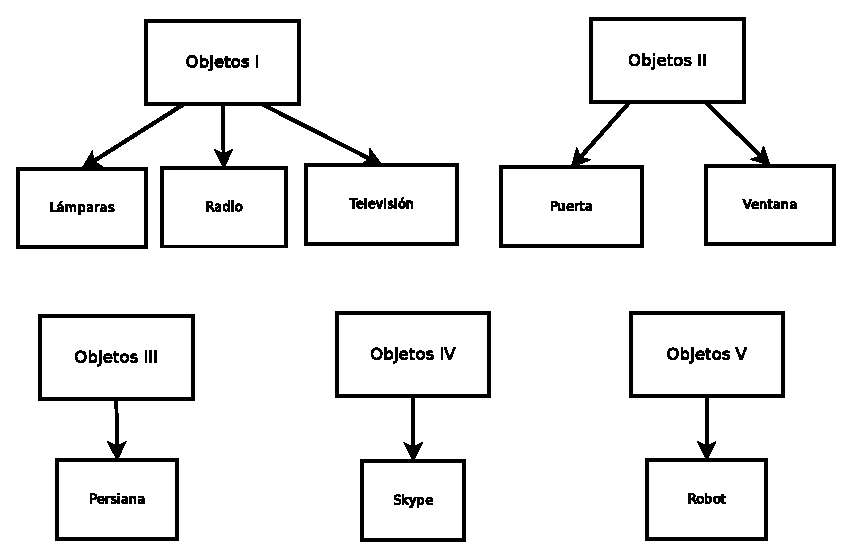
\includegraphics{Esquema_objetos}
  \caption{Clasificación de los objetos para la gramática; los pies de figura también pueden contener acrónimos como \acs{ETTS} y símbolos como \ac{xidet}.}
  \label{fig:fig_clobj}
\end{figure}

Incluye en todas las figuras un pie descriptivo y una etiqueta única mediante \texttt{\textbackslash{}label}. Para citarlas desde el texto, utiliza \texttt{\textbackslash{}ref}, preferiblemente acompañado del tipo de elemento, como en \texttt{figura\textasciitilde{}\textbackslash{}ref\{fig:fig\_clobj\}}.

\section{Definición y uso de acrónimos}
\label{sec:uso-de-acronimos}

La plantilla gestiona los acrónimos mediante el paquete \texttt{glossaries}. Sus definiciones se encuentran en \texttt{acronyms/defacronymsgl.tex}, mientras que \texttt{acronyms/acronymsgl.tex} configura y genera el listado correspondiente.

Puedes definir un acrónimo mediante una orden como:

\begin{verbatim}
\newacronym{ETTS}{ETTS}{Emotional Text To Speech}
\end{verbatim}

La orden \texttt{\textbackslash{}ac\{ETTS\}} produce \ac{ETTS} y gestiona automáticamente la forma mostrada en usos posteriores. Las principales órdenes disponibles en los ejemplos son:

\begin{itemize}
  \item \texttt{\textbackslash{}ac\{clave\}}: utiliza la forma completa la primera vez y la abreviada en los usos posteriores.
  \item \texttt{\textbackslash{}acs\{clave\}}: fuerza la forma abreviada.
  \item \texttt{\textbackslash{}acl\{clave\}}: fuerza la forma desarrollada.
  \item \texttt{\textbackslash{}acf\{clave\}}: fuerza la forma completa, con la abreviatura incluida.
  \item \texttt{\textbackslash{}acp\{clave\}}: utiliza la forma plural configurada para el acrónimo.
  \item \texttt{\textbackslash{}glsresetall[acronym]}: reinicia el estado de uso de todos los acrónimos para que vuelvan a tratarse como no utilizados.
\end{itemize}

Para que puedas ver el mecanismo en funcionamiento, reiniciamos primero el estado de los acrónimos:

\glsresetall[acronym]

Si ahora nos referimos a \ac{ETTS}, aparecerá su forma desarrollada por tratarse del primer uso; al volver a escribir \ac{ETTS}, se mostrará únicamente el acrónimo. También puedes forzar la forma abreviada con \acs{EMODB}, la forma desarrollada con \acl{EMODB} o la forma completa con \acf{EMODB}.

Puedes definir mediante \texttt{\textbackslash{}newglossaryentry} las entradas que necesiten plurales personalizados u otros atributos, como muestra el acrónimo \texttt{SOC} incluido en el fichero de ejemplo. Para generar el listado, ejecuta \texttt{makeglossaries}, tal como se explica en la sección~\ref{sec:compilacion}.

También puedes comprobar cómo se gestionan los plurales: la primera aparición de \acp{SOC} utiliza la forma desarrollada configurada y, al repetir \acp{SOC}, se muestra su forma abreviada plural. Después podemos volver al singular mediante \ac{SOC}.

\section{Definición y uso de símbolos}
\label{sec:simbolos}

Los símbolos se gestionan también mediante \texttt{glossaries}. Se definen en \texttt{symbols/defsymbolsgl.tex} como entradas del glosario de tipo \texttt{symbols}, y su listado se configura en \texttt{symbols/symbolsgl.tex}.

Los ejemplos incluidos representan el ángstrom, \ac{angstrom}; el ohmio, \ac{ohm}; una señal de audio, \ac{xdet}; una señal capturada por el micrófono \(i\), \ac{xidet}; y la independencia condicional, \ac{condindep}. Puedes utilizar la orden \texttt{\textbackslash{}ac\{clave\}} tanto con acrónimos como con estas entradas de símbolos.

Las definiciones permanecen disponibles aunque ocultes sus listas. Utiliza \texttt{\textbackslash{}myIncludeListOfAcronyms} y \texttt{\textbackslash{}myIncludeListOfSymbols} en \texttt{Config/myconfig.tex} para decidir si aparecen esas páginas. Si no utilizas acrónimos ni símbolos tampoco necesitarás ejecutar \texttt{makeglossaries}; la sección~\ref{sec:compilacion} explica cuándo debes incorporar esta herramienta al proceso de compilación.

\section{Enlaces a vídeos y listados adicionales}
\label{sec:intro-videolink}

En marzo de 2023 recibimos una pregunta sobre la posibilidad de incluir enlaces a vídeos en el documento y generar automáticamente un listado similar al de tablas, figuras o algoritmos. El código para implementarlo está en el fichero \texttt{cover/extralistings.tex}, que puedes editar y adaptar a tus necesidades.

Puedes añadir un enlace mediante una orden como:

\begin{verbatim}
\videoLink{Título descriptivo del vídeo}{https://example.org/video}
\end{verbatim}

Para usarlo, basta con que incluyas elementos similares a \videoLink{Introducción al Laboratorio de Circuitos Electrónicos (I)}{https://www.youtube.com/watch?v=U1P2ZP0f8KM} o \videoLink{Introducción al Laboratorio de Circuitos Electrónicos (V)}{https://www.youtube.com/watch?v=nPsxMqKRGx0}. La orden incorpora el enlace al texto y registra la entrada en el listado de vídeos. Para mostrar ese listado, asigna el valor \texttt{true} a \texttt{\textbackslash{}myIncludeListOfVideos} en \texttt{Config/myconfig.tex}.

Lo importante no es tanto que sea un listado de vídeos, sino que este ejemplo muestra cómo se pueden integrar listados de elementos adicionales que sean a su vez enlaces y configurar la generación del índice para crear enlaces visitables desde el propio índice, además de su indexación convencional.

\section{Resumen del capítulo}
\label{sec:resumen-elementos-utilidad}

La plantilla proporciona comandos reutilizables, entornos para frases, rutas preparadas para figuras y diagramas, gestión de acrónimos y símbolos, y un ejemplo de listados con enlaces a vídeos. Conserva y adapta únicamente los recursos que resulten útiles para tu documento, comprobando sus usos antes de eliminar cualquier definición.

%%% Local Variables:
%%% TeX-master: "../book"
%%% End:

%%%%%%%%%%%%%%%%%%%%%%%%%%%%%%%%%%%%%%%%%%%%%%%%%%%%%%%%%%%%%%%%%%%%%%%%%%%
% Función: documentos complementarios.
%
% Uso: modifica este fichero para adaptar el contenido a tu trabajo.
%%%%%%%%%%%%%%%%%%%%%%%%%%%%%%%%%%%%%%%%%%%%%%%%%%%%%%%%%%%%%%%%%%%%%%%%%%%

\chapter{Documentos complementarios}
\label{cha:documentos-complementarios}

Además del libro principal, hemos incluido una plantilla de anteproyecto y varios documentos administrativos que reutilizan la configuración común. En este capítulo te explicamos qué contiene cada directorio y cómo puedes generar únicamente los documentos que necesites.

\section{Plantilla de anteproyecto}
\label{sec:plantilla-de-anteproyecto}

Para ayudarte a preparar la propuesta inicial de un TFC, TFG o TFM, hemos incluido una plantilla simplificada en el directorio \texttt{Anteproyecto/}. Su fichero principal es \texttt{Anteproyecto/anteproyecto.tex} y reutiliza los datos que hayas definido en \texttt{Config/myconfig.tex}, incluidos el tipo de trabajo, la titulación, el título, la autoría, los tutores, el departamento y la fecha de propuesta.

El contenido de ejemplo está organizado en secciones de introducción, objetivos, metodología, plan de trabajo y bibliografía. Adapta estas secciones a los requisitos de tu titulación; puedes ampliarlas, eliminarlas o reordenarlas libremente.

Puedes compilar el anteproyecto con cualquier editor o herramienta habitual de \LaTeX{}. También hemos incluido un \texttt{Makefile}, que puedes ejecutar mediante:

\begin{verbatim}
cd Anteproyecto
make
\end{verbatim}

La compilación genera \texttt{anteproyecto.pdf}. El \texttt{Makefile} utiliza \texttt{latexmk} para controlar las dependencias, ejecutar Biber y las pasadas de \texttt{pdflatex} que sean necesarias, y evitar la recompilación cuando ninguna fuente ha cambiado.

Si trabajas en Overleaf, sigue el procedimiento de la sección~\ref{sec:compilacion-overleaf} y selecciona \texttt{Anteproyecto/anteproyecto.tex} como documento principal.

El \texttt{Makefile} también proporciona los objetivos \texttt{snapshot}, \texttt{flatten}, \texttt{latexdiff}, \texttt{clean}, \texttt{cleanall} y \texttt{help}. Los nombres \texttt{anteproyecto\_latexmk} y \texttt{clean\_latexmk} se conservan como alias compatibles de \texttt{anteproyecto} y \texttt{cleanall}, respectivamente. Los objetivos de revisión siguen el mismo principio que los equivalentes del libro principal, descritos en la sección~\ref{sec:control-de-cambios}.

\section{Caso especializado: tesis por compendio de publicaciones}
\label{sec:tesis-compendio}

Esta sección está destinada únicamente a estudiantes de doctorado que presenten su tesis por compendio de publicaciones; el resto de usuarios debe mantener la estructura \texttt{standard} y trabajar con \texttt{Book/content-standard.tex}. Para el caso especializado, utiliza \texttt{Book/book.tex} como documento principal, selecciona \texttt{compendium} como valor de \texttt{\textbackslash{}myDocumentStructure} y elige con \texttt{\textbackslash{}myDegree} un programa de doctorado admitido. La plantilla genera un error si intentas combinar esta estructura con un TFG, TFM u otro tipo de trabajo.

La organización especializada se define en \texttt{Book/content-compendium.tex}. Su primera parte contiene el resumen extendido de la tesis y utiliza los ficheros \texttt{introduction.tex}, \texttt{objectives.tex}, \texttt{previous-work.tex}, \texttt{methodology.tex}, \texttt{thesis-contributions.tex} y \texttt{conclusions.tex} del directorio \texttt{Book/chapters/compendium/}. Puedes ampliar, combinar o reordenar esta propuesta según las necesidades de la tesis. La bibliografía se imprime al final de esta primera parte, antes de comenzar la relación de publicaciones.

La segunda parte incorpora las publicaciones en su formato original. Guarda sus PDF definitivos en \texttt{Book/publications/} y añade una llamada por publicación en \texttt{Book/content-compendium.tex}. La orden proporcionada tiene la forma siguiente:

\begin{verbatim}
\includecompendiumpublication[
  Información adicional con formato LaTeX.
]{etiqueta}
 {Título breve para el índice}
 {Título completo de la publicación}
 {clave-bibliográfica}
 {publications/publication-file.pdf}
\end{verbatim}

La orden crea un capítulo numerado y su entrada en el índice, imprime mediante BibLaTeX la referencia correspondiente, muestra la información adicional cuando se proporciona e incluye todas las páginas del PDF con la escala configurada en \texttt{Config/preamble.tex}. En esas páginas mantiene la numeración de la tesis y utiliza como cabecera el título abreviado indicado en el segundo argumento obligatorio. El argumento opcional admite órdenes habituales de \LaTeX{}, párrafos, enlaces, referencias y listas; puedes omitirlo por completo cuando no tengas que indicar el estado de publicación, la contribución del doctorando, los permisos de reutilización u otra información específica. Los autores, la revista o congreso, la fecha y el DOI deben mantenerse en la entrada de \texttt{biblio/biblio.bib} para no duplicarlos en la llamada.

Selecciona siempre \texttt{Book/book.tex} como documento principal si trabajas desde tu editor o desde Overleaf. Si utilizas \texttt{make}, ejecuta el objetivo normal \texttt{make} desde \texttt{Book/}; la estructura elegida en \texttt{myconfig.tex} utiliza la misma secuencia de PDFLaTeX, Biber y glosarios. Antes de depositar la tesis, comprueba tanto la normativa doctoral aplicable como los derechos de reutilización de cada publicación.

\section{Documentación administrativa}
\label{sec:introapp1}

Para evitar que tengas que introducir varias veces los mismos datos, hemos preparado en los directorios \texttt{PapeleoTFG/}, \texttt{PapeleoTFM/} y \texttt{PapeleoPHD/} distintos documentos administrativos que reutilizan la información definida en \texttt{Config/myconfig.tex}. Antes de generarlos, asegúrate de completar especialmente los datos de autoría, tutores, tribunal, fechas, calificaciones y publicación en abierto que correspondan a cada formulario.

\subsection{Documentos para TFG}

El directorio \texttt{PapeleoTFG/} contiene actualmente:

\begin{itemize}
  \item \texttt{TFG-AutorizacionALLPubAbierto-EPS-UAH.tex}: autorización conjunta del estudiante, el tutor y, cuando exista, el cotutor para publicar el TFG en abierto.
  \item \texttt{TFG-AutorizacionAutorPubAbierto-EPS-UAH.tex}: declaración y autorización de la persona autora para la publicación en abierto.
  \item \texttt{TFG-AutorizacionTutorExtranjeroPubAbierto-EPS-UAH.tex}: autorización en inglés para un tutor perteneciente a una universidad extranjera.
  \item \texttt{TFG-CompromisoConfidencialidad-EPS-UAH.tex}: compromisos individuales de confidencialidad del tutor, el cotutor y los miembros configurados del tribunal.
  \item \texttt{TFG-ConvenioCooperacion-EPS-UAH.tex}: anexo para realizar el TFG mediante un convenio de cooperación educativa.
  \item \texttt{TFG-InformeTutorYRubrica-EPS-UAH.tex}: informe y rúbrica del tutor o tutores.
  \item \texttt{TFG-InformeTutorPlagio-UAH.tex}: informe del tutor sobre la revisión de plagio.
  \item \texttt{TFG-ActaYRubricaDefensa-EPS-UAH.tex}: acta y rúbrica del tribunal de defensa.
\end{itemize}

El \texttt{Makefile} de este directorio compila todos los formularios independientes y genera un PDF por cada uno; los restantes ficheros \texttt{.tex} son fragmentos auxiliares incluidos por esos formularios y no deben compilarse por separado. También puedes abrir y compilar individualmente el documento que necesites con tu editor o herramienta de \LaTeX{} preferidos.

\subsection{Documentos para TFM}

El directorio \texttt{PapeleoTFM/} contiene actualmente:

\begin{itemize}
  \item \texttt{TFM-AutorizacionPublicarAbierto.tex}: formulario de autorización para la publicación en abierto, con los datos de la persona autora, el tutor y, cuando exista, el cotutor.
  \item \texttt{TFM-VistoBuenoTutor.tex}: visto bueno del tutor o tutores para el depósito y la defensa del TFM. Para el MUIE también refleja si el trabajo está sujeto a confidencialidad.
  \item \texttt{TFM-AnexoI-ConvenioCooperacion-EPS-UAH.tex}: anexo para realizar el TFM mediante un convenio de cooperación educativa.
  \item \texttt{TFM-ActaYRubricaDefensa-EPS-UAH.tex}: acta y rúbrica del tribunal de defensa.
  \item \texttt{TFM-AnexoIV-SolicitudProrroga-EPS-UAH.tex}: solicitud de prórroga del plazo de entrega del TFM.
  \item \texttt{TFM-AnexoV-SolicitudCambioTFM-EPS-UAH.tex}: solicitud de cambio del TFM asignado.
\end{itemize}

El \texttt{Makefile} de este directorio compila todos los ficheros \texttt{.tex} y genera sus correspondientes PDF. También puedes compilar cada formulario por separado mediante tu editor o una herramienta estándar de \LaTeX{}.

\subsection{Documentos para tesis doctorales}

El directorio \texttt{PapeleoPHD/} contiene \texttt{PHD-VistoBuenoTutorTesis.tex}, una plantilla de visto bueno de los directores para la defensa de una tesis doctoral. También conserva \texttt{vistoBuenoDirectoresTesis\_plantilla.doc} como documento institucional de referencia.

Puedes compilar el documento \texttt{PHD-VistoBuenoTutorTesis.tex} directamente con \texttt{pdflatex}, desde un editor de \LaTeX{} o mediante el \texttt{Makefile} incluido en el directorio.

\subsection{Compilación y revisión de los formularios}

Desde cualquiera de los directorios \texttt{PapeleoTFG/}, \texttt{PapeleoTFM/} y \texttt{PapeleoPHD/} puedes generar todos los formularios disponibles mediante:

\begin{verbatim}
make
\end{verbatim}

El uso de \texttt{make} es opcional y requiere \texttt{latexmk}. Cada invocación comprueba las dependencias registradas y solo repite las pasadas de \texttt{pdflatex} cuando ha cambiado alguna fuente directa o alguno de los ficheros compartidos de \texttt{Config/}. También puedes compilar cada fichero individualmente con dos pasadas de \texttt{pdflatex} o mediante la función de construcción de tu editor de \LaTeX{} preferido. Estos formularios no utilizan la bibliografía ni los glosarios del libro principal.

Si solo necesitas un formulario, puedes indicar directamente el nombre del PDF, por ejemplo \texttt{make TFG-InformeTutorYRubrica-EPS-UAH.pdf}. Los dos directorios utilizan la misma organización de objetivos: \texttt{autorizaciones} genera las autorizaciones y documentos afines, \texttt{convenios} genera los formularios de cooperación educativa y \texttt{evaluacion} genera los informes, actas y rúbricas. En \texttt{PapeleoTFM/} también puedes utilizar \texttt{solicitudes} para generar las solicitudes de prórroga y cambio de TFM. El objetivo \texttt{help} de cada directorio muestra las opciones disponibles.

El objetivo \texttt{clean} elimina únicamente los ficheros auxiliares de la compilación y conserva los PDF generados; utiliza \texttt{cleanall} cuando también quieras eliminar esos PDF.

Desde la raíz del repositorio puedes ejecutar \texttt{make paperwork} para generar únicamente el conjunto de formularios que corresponde a la titulación seleccionada en \texttt{myconfig.tex}. El objetivo \texttt{make all-documents} añade además el README, el libro principal y el anteproyecto; el objetivo predeterminado de la raíz no cambia y continúa generando únicamente el README y el libro.

En Overleaf puedes generar cada formulario seleccionando su fichero \texttt{.tex} como documento principal, de acuerdo con las indicaciones de la sección~\ref{sec:compilacion-overleaf}.

Las plantillas adaptan automáticamente determinados términos al género gramatical configurado y omiten los datos del cotutor cuando \texttt{\textbackslash{}myCoTutorFullName} está vacío. Aun así, revisa cuidadosamente el PDF resultante, las firmas requeridas y la coherencia de todos los datos.

Los modelos administrativos y sus requisitos pueden cambiar. Antes de presentar cualquiera de estos documentos, comprueba que su contenido coincida con la normativa y los formularios oficiales vigentes de tu titulación.


\section{Resumen del capítulo}
\label{sec:resumen-documentos-complementarios}

El anteproyecto, la tesis por compendio y los formularios administrativos reutilizan la configuración común para evitar que introduzcas varias veces los mismos datos. Puedes compilarlos independientemente del libro ordinario, también mediante Overleaf si seleccionas el documento principal adecuado, pero debes revisar cada PDF y contrastar siempre las plantillas con los requisitos y modelos oficiales vigentes antes de presentarlos.

%%% Local Variables:
%%% TeX-master: "../book"
%%% End:

%%%%%%%%%%%%%%%%%%%%%%%%%%%%%%%%%%%%%%%%%%%%%%%%%%%%%%%%%%%%%%%%%%%%%%%%%%%
%
% Generic template for TFC/TFM/TFG/Tesis
%
% By:
%  + Javier Macías-Guarasa.
%    Departamento de Electrónica
%    Universidad de Alcalá
%  + Roberto Barra-Chicote.
%    Departamento de Ingeniería Electrónica
%    Universidad Politécnica de Madrid
%
% By: + Javier Macías-Guarasa. Departamento de Electrónica Universidad de Alcalá + Roberto Barra-Chicote. Departamento de Ingeniería Electrónica Universidad Politécnica de Madrid
%
% Based on original sources by Roberto Barra, Manuel Ocaña, Jesús Nuevo, Pedro Revenga, Fernando Herránz and Noelia Hernández. Thanks a lot to all of them, and to the many anonymous contributors found (thanks to google) that provided help in setting all this up.
%
% See also the additionalContributors.txt file to check the name of additional contributors to this work.
%
% If you think you can add pieces of relevant/useful examples, improvements, please contact us at (macias@depeca.uah.es)
%
% You can freely use this template and please contribute with comments or suggestions!!!
%
%%%%%%%%%%%%%%%%%%%%%%%%%%%%%%%%%%%%%%%%%%%%%%%%%%%%%%%%%%%%%%%%%%%%%%%%%%%

\chapter{Compilación y herramientas avanzadas}
\label{cha:compilacion-avanzada}

No necesitas las herramientas de este capítulo para comenzar a escribir o para compilar el documento desde tu editor. Las hemos reunido aquí para que puedas automatizar tareas, preparar revisiones y diagnosticar problemas cuando tu forma de trabajo las requiera.

\section{Compilación mediante el \texttt{Makefile}}
\label{sec:compilacion-makefile}

Para facilitar la generación del documento incluimos un \texttt{Makefile}. No somos expertos ni en \texttt{make} ni en \LaTeX{}, así que seguramente no sea el mejor \texttt{Makefile} del mundo, pero creemos que cumple su función y puede servir también como ejemplo para adaptar el proceso de compilación a tus necesidades.

El objetivo predeterminado \texttt{all}, ejecutado al invocar \texttt{make} sin argumentos, convierte primero los diagramas y figuras que lo necesiten. A continuación ejecuta \texttt{pdflatex}, Biber, \texttt{makeglossaries} y las dos pasadas finales de \texttt{pdflatex}. Dado que el libro de ejemplo utiliza acrónimos y símbolos, el \texttt{Makefile} ejecuta siempre \texttt{makeglossaries}.

La compilación genera \texttt{book.pdf} y \texttt{book-compressed.pdf}. También crea copias cuyos nombres identifican el tipo de trabajo, la titulación, el autor y el idioma configurados. La versión comprimida utiliza la configuración \texttt{/prepress} de Ghostscript; la antigua versión de calidad \texttt{/screen} está desactivada porque degradaba excesivamente las imágenes.

El objetivo \texttt{all} también actualiza el fichero \texttt{RELEASE.txt} con la etiqueta más reciente del repositorio e intenta añadirlo al índice de Git. Por tanto, después de compilar, revisa el estado del repositorio antes de preparar un commit.

Para el uso habitual de la plantilla solo necesitarás los siguientes objetivos:

\begin{itemize}
  \item \texttt{all}: compila el documento completo y genera las copias finales; es el objetivo ejecutado de forma predeterminada por \texttt{make}.
  \item \texttt{clean}: elimina los ficheros auxiliares y los PDF de trabajo generados durante la compilación.
\end{itemize}

Los siguientes objetivos proporcionan operaciones avanzadas para la revisión y la preparación del proyecto:

\begin{itemize}
  \item \texttt{all\_latexmk}: ofrece un procedimiento alternativo y experimental de compilación basado en \texttt{latexmk}.
  \item \texttt{clean\_latexmk}: elimina los ficheros auxiliares mediante \texttt{latexmk} y completa después la limpieza de otros ficheros generados.
  \item \texttt{snapshot}: genera mediante \texttt{latexpand} una copia unificada del documento que puede utilizarse como referencia para una revisión posterior.
  \item \texttt{flatten}: genera una copia unificada del estado actual del documento.
  \item \texttt{latexdiff}: compara la instantánea con el estado actual y genera un PDF que muestra las diferencias.
  \item \texttt{backup-chapters}: crea copias fechadas de los capítulos convencionales, los apéndices, \texttt{content-standard.tex} y \texttt{myconfig.tex}.
  \item \texttt{orig-standard}: selecciona la estructura \texttt{standard}, sustituye los capítulos, apéndices y \texttt{content-standard.tex} por las versiones completas del manual y reactiva sus elementos opcionales después de crear una copia de seguridad; \texttt{orig-chapters} se conserva como alias compatible.
  \item \texttt{bare-standard}: selecciona la estructura normal \texttt{standard}, instala los capítulos, apéndices y \texttt{content-standard.tex} mínimos y desactiva el material opcional de ejemplo; \texttt{bare-chapters} se conserva como alias de este objetivo.
  \item \texttt{bare}: utiliza normalmente \texttt{bare-standard}; si un estudiante de doctorado ha seleccionado expresamente \texttt{compendium}, prepara en su lugar la estructura especializada. Después ofrece eliminar los gráficos y diagramas existentes.
  \item \texttt{backup-compendium}: crea una copia fechada de los capítulos especializados, \texttt{content-compendium.tex} y \texttt{myconfig.tex}.
  \item \texttt{bare-compendium}: selecciona la estructura especializada \texttt{compendium}, instala sus seis capítulos y \texttt{content-compendium.tex} mínimos, y desactiva el material opcional de ejemplo.
  \item \texttt{orig-compendium}: selecciona la estructura \texttt{compendium}, restaura sus seis capítulos completos y \texttt{content-compendium.tex} desde \texttt{chapters/compendium/orig/}, y reactiva el material opcional de ejemplo.
  \item \texttt{orig}: consulta \texttt{\textbackslash{}myDocumentStructure} y ejecuta \texttt{orig-standard} u \texttt{orig-compendium} según corresponda.
\end{itemize}

Los objetivos relacionados con la comparación de versiones se explican con más detalle en la sección~\ref{sec:control-de-cambios}.

El \texttt{Makefile} contiene además objetivos auxiliares utilizados internamente para convertir recursos y preparar la versión mínima. No necesitas ejecutarlos directamente.

Los objetivos \texttt{bare}, \texttt{bare-standard}, \texttt{bare-compendium}, \texttt{bare-chapters}, \texttt{orig}, \texttt{orig-standard}, \texttt{orig-compendium} y \texttt{orig-chapters} modifican los directorios de capítulos, los apéndices cuando corresponda, el fichero \texttt{content-*.tex} seleccionado y la configuración almacenada en \texttt{myconfig.tex}. Todos crean primero la copia de seguridad correspondiente y no reescriben \texttt{book.tex}. Además, \texttt{bare} puede eliminar los ficheros de \texttt{figures/} y \texttt{diagrams/} si se confirma expresamente durante su ejecución. Utilízalos únicamente al preparar una copia nueva del proyecto y después de comprobar que los cambios importantes están guardados en el sistema de control de versiones.

Algunos objetivos del \texttt{Makefile} utilizan herramientas adicionales. Solo necesitas instalar las que correspondan a los objetivos que vayas a utilizar:

\begin{itemize}
  \item \texttt{Ghostscript}: genera la copia comprimida del documento cuando se utiliza el objetivo \texttt{all} del \texttt{Makefile}.
  \item \texttt{Inkscape}: convierte automáticamente los diagramas en formato \texttt{svg} a \texttt{pdf}.
  \item \texttt{Dia} y \texttt{epspdf}: convierten automáticamente los diagramas en formato \texttt{dia} a \texttt{pdf}; \texttt{epspdf} también convierte las figuras en formato \texttt{eps} a \texttt{pdf}.
  \item \texttt{latexmk}: proporciona el procedimiento alternativo utilizado por los objetivos \texttt{all\_latexmk} y \texttt{clean\_latexmk}.
  \item \texttt{latexpand} y \texttt{latexdiff}: permiten unificar los fuentes y generar documentos que muestran las diferencias entre dos versiones.
  \item \texttt{Perl}: es necesario para ejecutar \texttt{makeglossaries} en los sistemas que no incluyan ya un intérprete compatible.
\end{itemize}

Instala estas herramientas solo cuando vayas a utilizar la prestación correspondiente. No son requisitos para redactar ni compilar un documento básico que no dependa de ellas.


\section{Generación del documento con control de cambios}
\label{sec:control-de-cambios}

Uno de los problemas que encontramos al trabajar con \LaTeX{} aparece durante la revisión: después de entregar un borrador, el tutor o director puede querer comprobar cómo se han incorporado sus sugerencias. En un procesador de textos como LibreOffice (vaaaaaaaaale, o Microsoft Word también) resulta habitual activar el control de cambios o comparar dos documentos; con \LaTeX{} también podemos obtener un resultado equivalente mediante algunas herramientas adicionales.

Para ello utilizamos \texttt{latexdiff}, que compara dos versiones de un documento \LaTeX{} y genera un nuevo fichero en el que se marcan visualmente las inserciones y eliminaciones. Al compilarlo obtenemos un PDF independiente mucho más cómodo para revisar que un \texttt{diff} a palo seco de los ficheros fuente.

Como el libro se divide mediante múltiples órdenes \texttt{\textbackslash{}input}, antes de realizar la comparación se utiliza \texttt{latexpand} para generar una versión unificada. El \texttt{Makefile} de \texttt{Book/} automatiza este procedimiento mediante los objetivos \texttt{snapshot}, \texttt{flatten} y \texttt{latexdiff}.

\subsection{Creación de la versión de referencia}

Cuando tengas una versión que quieras utilizar como base de la revisión, ejecuta desde el directorio \texttt{Book/}:

\begin{verbatim}
make snapshot
\end{verbatim}

Este objetivo genera \texttt{book-flatten-snapshot.tex}, que contiene en un solo fichero el estado expandido del documento. Crea la instantánea antes de comenzar las modificaciones que quieras mostrar y consérvala sin cambios durante el proceso de revisión.

Si utilizas Git, te recomendamos registrar la instantánea junto con la versión del documento a la que corresponde:

\begin{verbatim}
git add book-flatten-snapshot.tex
git commit -m "chore: update the review snapshot"
\end{verbatim}

El objetivo \texttt{snapshot} sobrescribe la instantánea existente. Por tanto, no vuelvas a ejecutarlo hasta que quieras establecer una nueva versión de referencia.

\subsection{Generación del documento de diferencias}

Después de modificar el documento, puedes generar la comparación mediante:

\begin{verbatim}
make latexdiff
\end{verbatim}

El objetivo \texttt{latexdiff} genera primero \texttt{book-flatten.tex} con el estado actual, lo compara con \texttt{book-flatten-snapshot.tex} y crea \texttt{book-flatten-diff.tex}. A continuación procesa su bibliografía y sus glosarios y genera \texttt{book-flatten-diff.pdf}, que contiene las diferencias resaltadas.

La comparación depende de que exista previamente \texttt{book-flatten-snapshot.tex}. Si quieres iniciar un nuevo ciclo de revisión, comprueba primero que hayas guardado los cambios anteriores y ejecuta de nuevo \texttt{make snapshot} para reemplazar la versión de referencia.

El \texttt{Makefile} aplica además una corrección específica al resultado de \texttt{latexdiff} para tratar determinados entornos de TikZ utilizados por la plantilla. Esta corrección ayuda con los ejemplos actuales, pero un documento que contenga construcciones complejas puede requerir ajustes manuales en \texttt{book-flatten-diff.tex}.

\subsection{Uso sin \texttt{make}}

El flujo de revisión no requiere obligatoriamente la utilidad \texttt{make}. Cristina Losada aportó un procedimiento para utilizar \texttt{latexdiff} directamente en Windows, que también puede adaptarse a otros sistemas operativos:

\begin{enumerate}
  \item Instala \texttt{latexdiff} y un intérprete de Perl. MiKTeX incluye \texttt{latexdiff}, y Strawberry Perl es una de las alternativas disponibles para Windows.
  \item Guarda una copia del documento que utilizarás como referencia; por ejemplo, \texttt{book-snapshot.tex}.
  \item Realiza las modificaciones necesarias en el documento.
  \item Ejecuta desde el directorio \texttt{Book/}:
\end{enumerate}

\begin{verbatim}
latexdiff --flatten book-snapshot.tex book.tex > book-flatten-diff.tex
\end{verbatim}

Después, compila \texttt{book-flatten-diff.tex}. Si la versión comparada contiene bibliografía, acrónimos o símbolos, ejecuta también Biber y \texttt{makeglossaries} con el nombre base \texttt{book-flatten-diff}, seguidos de las pasadas adicionales de \texttt{pdflatex}.

Este procedimiento manual compara directamente el documento guardado con la versión actual. Para que \texttt{--flatten} pueda expandir correctamente ambos documentos, conserva también los ficheros incluidos por cada versión o utiliza copias ya unificadas mediante \texttt{latexpand}.

También existen otras alternativas integradas con Git, como \texttt{git-latexdiff}~\cite{git-latexdiff}. El procedimiento incluido en este repositorio no depende de una herramienta concreta de control de versiones, aunque te recomendamos utilizar Git u otro sistema equivalente para conservar el historial de tu trabajo.

\section{Resolución de problemas}
\label{sec:problemas-conocidos}

Los problemas observados antiguamente con Ubuntu 12.04, el paquete \texttt{xcolor}, Evince y Xpdf ya no describen entornos actuales y se han retirado de esta guía. Si una compilación falla, localiza el primer error del registro, ya que muchos de los mensajes posteriores suelen ser consecuencias de ese fallo inicial.

Las comprobaciones más habituales son:

\begin{itemize}
  \item Si falta un fichero \texttt{.sty}, instala el paquete correspondiente desde la distribución de \LaTeX{} que utilices.
  \item Si no aparece la bibliografía o las citas quedan sin resolver, comprueba que hayas ejecutado Biber y realiza después las pasadas adicionales de \texttt{pdflatex}.
  \item Si no aparecen los listados de acrónimos o símbolos, ejecuta \texttt{makeglossaries} antes de las pasadas finales de \texttt{pdflatex}.
  \item Si falla la conversión de un fichero \texttt{dia}, \texttt{svg} o \texttt{eps}, instala la herramienta opcional correspondiente o proporciona directamente una versión compatible en \texttt{pdf}, \texttt{png} o \texttt{jpg}.
  \item Si las referencias cruzadas o los índices no están actualizados, repite las pasadas de \texttt{pdflatex}; antes de recompilar también puedes utilizar \texttt{make clean} para eliminar los auxiliares anteriores.
  \item Si \texttt{latexdiff} genera un fichero que no compila, revisa el primer error de \texttt{book-flatten-diff.tex}. Las tablas, fórmulas, entornos TikZ y órdenes personalizadas pueden necesitar correcciones manuales en el documento de diferencias.
  \item Si una cubierta o un formulario no coincide con el modelo institucional esperado, comprueba \texttt{\textbackslash{}myDegree}, el idioma, los datos compartidos y la normativa vigente antes de modificar directamente la plantilla.
\end{itemize}

Cuando nos comuniques un problema, incluye el sistema operativo, la distribución y versión de \LaTeX{}, la titulación seleccionada, el comando de compilación y el primer error relevante del fichero de registro. También puedes proponer correcciones mediante el repositorio del proyecto.

Si encuentras algún otro problema, escribe a \contactauthor{} para contárnoslo y trataremos de solucionarlo. Y si ya has encontrado una solución, no dudes en compartirla: tu contribución puede ser útil para quienes utilicen la plantilla después.


\section{Resumen del capítulo}
\label{sec:resumen-compilacion-avanzada}

El \texttt{Makefile} puede automatizar la compilación, la conversión de recursos y la preparación de versiones con cambios, pero sigue siendo opcional y no sustituye a las herramientas de tu editor. Cuando surja un problema, identifica el primer error del registro y aporta la información del entorno necesaria para poder reproducirlo.

%%% Local Variables:
%%% TeX-master: "../book"
%%% End:

%%%%%%%%%%%%%%%%%%%%%%%%%%%%%%%%%%%%%%%%%%%%%%%%%%%%%%%%%%%%%%%%%%%%%%%%%%%
% Función: ejemplos de elementos básicos de LaTeX.
%
% Uso: modifica este fichero para adaptar el contenido a tu trabajo.
%%%%%%%%%%%%%%%%%%%%%%%%%%%%%%%%%%%%%%%%%%%%%%%%%%%%%%%%%%%%%%%%%%%%%%%%%%%

\chapter{Elementos básicos de \LaTeX{}}
\label{cha:elementos-basicos}

\begin{FraseCelebre}
  \begin{Frase}
    Y así, del mucho leer y del poco dormir, se le secó el cerebro de manera que vino a perder el juicio\footnote{Tomado de ejemplos del proyecto \texis{}.}.
  \end{Frase}
  \begin{Fuente}
    Miguel de Cervantes Saavedra
  \end{Fuente}
\end{FraseCelebre}

En este capítulo reunimos ejemplos de los elementos de \LaTeX{} que utilizarás con más frecuencia. Veremos estructuras, listas y citas, expresiones matemáticas y referencias cruzadas, niveles de organización, figuras y tablas; puedes acudir directamente al apartado que necesites.

\section{Estructura, listas y citas}
\label{sec:estructura-listas-citas}

Este capítulo reúne ejemplos breves de elementos habituales de \LaTeX{}. Puedes consultar directamente sus fuentes y adaptar únicamente los fragmentos que necesites.

Una lista sin numerar puede construirse mediante el entorno \texttt{itemize}:

\begin{itemize}
  \item Primer elemento de ejemplo.
  \item Segundo elemento de ejemplo.
\end{itemize}

Las fuentes bibliográficas se citan con \texttt{\textbackslash{}cite\{\}} (no olvides usar un espacio inseparable ``\~'' entre el texto previo y el comando \texttt{\textbackslash{}cite\{\}}). Por ejemplo, esta plantilla describe el proyecto \texis{} en~\cite{texis}. También puedes añadir una aclaración mediante una nota al pie\footnote{Este es un ejemplo de nota al pie.}.

En algunas ocasiones puedes querer mostrar una referencia bibliográfica completa en el propio texto sin repetirla después en la bibliografía final. Por ejemplo, la orden \texttt{\textbackslash{}fullcite} nos permite incorporar directamente la siguiente referencia en el texto (por ejemplo cuando estás listando las publicaciones resultado de tu tesis doctoral):

\fullcite{monasterio2022}

Para conseguirlo, hemos guardado esta entrada en \texttt{biblio/nobiblio.bib}, fichero declarado mediante \texttt{\textbackslash{}mybibfileTwo} en \texttt{biblio/bibliofiles.tex}, y hemos añadido dentro de la entrada la opción:

\begin{verbatim}
options = {skipbib=true}
\end{verbatim}

La opción \texttt{skipbib} permite utilizar la entrada con las órdenes de cita de \texttt{biblatex}, pero evita que aparezca cuando se imprime la bibliografía. Puedes utilizar este mecanismo para referencias que quieras presentar únicamente en el punto concreto del documento en el que se mencionan.

\section{Matemáticas y referencias cruzadas}
\label{sec:matematicas-referencias}

Puedes incluir expresiones matemáticas en línea, como $\sigma=0.75$, o utilizar un entorno independiente para una ecuación numerada:

\begin{equation}
  \label{eq:ejemplo-basico}
  p[q_t=\sigma_t\mid q_{t-1}=\sigma_{t-1}]
\end{equation}

La ecuación~\ref{eq:ejemplo-basico} muestra cómo asociar una etiqueta mediante \texttt{\textbackslash{}label} y recuperarla con \texttt{\textbackslash{}ref}. El mismo mecanismo se utiliza para capítulos, secciones, figuras, tablas, algoritmos y fragmentos de código.

Un asunto importante de formato, cuando utilices entornos \texttt{equation} y vayas a definir las variables utilizadas, fíjate en no dejar una línea en blanco entre la ecuación y el texto explicativo, para que no indente ese texto explicativo. Te pongo un ejemplo tomado de~\cite{ramirez2026jstars}:

\textit{On the other hand, for vessel localization, the regression model is evaluated using the {Mean Absolute Error (MAE)}. This measures the average absolute deviation between predictions and actual values (the lower, the better):}
\begin{equation}
  MAE = \frac{1}{\NumDataFrames{}} \sum_{i=1}^{\NumDataFrames{}} |y_i - \hat{y}_i|,
\end{equation}
\textit{where $\NumDataFrames$ is the number of data frames for which we generate a distance estimation value $\hat{y}_{i}$, and $y_{i}$ is the real distance.}


\section{Niveles de organización}
\label{sec:niveles-organizacion}

A continuación se muestran los niveles de división disponibles por debajo de un capítulo. Su aparición en el índice depende del valor configurado para \texttt{tocdepth}.


\subsection{Ejemplo de subsección}
\label{sec:subseccion}


\subsubsection{Ejemplo de subsubsección}
\label{sec:subsubseccion}

\paragraph{Ejemplo de párrafo}
\label{sec:paragraph-1}


\subparagraph{Ejemplo de subpárrafo}
\label{sec:subparagraph}

\subparagraph{Segundo ejemplo de subpárrafo}
\label{sec:subparagraph-2}

\paragraph{Segundo ejemplo de párrafo}
\label{sec:paragraph-2}

\subsubsection{Segundo ejemplo de subsubsección}
\label{sec:subsubseccion-2}

\subsection{Segundo ejemplo de subsección}
\label{sec:subseccion-2}

%%%%%%%%%%%%%%%%%%%%%%%%%%%%%%%%%%%%%%%%%%%%%%%%%%%%%%%%%%%%%%%%%%%%%%%%%%%
% Función: ejemplos de figuras y tablas.
%
% Uso: modifica este fichero para adaptar el contenido a tu trabajo.
%%%%%%%%%%%%%%%%%%%%%%%%%%%%%%%%%%%%%%%%%%%%%%%%%%%%%%%%%%%%%%%%%%%%%%%%%%%

\section{Figuras y tablas}
\label{sec:figuras-tablas}


\subsection{Figuras de uso habitual}
\label{sec:figuras-habituales}

Esta sección presenta ejemplos de figuras y tablas que pueden adaptarse a la mayoría de los documentos. Los casos que requieren una composición más elaborada se reúnen en el capítulo~\ref{cha:ejemplos-avanzados}.

La figura~\ref{fig:figura-convencional} muestra la inclusión habitual de una imagen con \texttt{figure}, \texttt{\textbackslash{}includegraphics}, un pie descriptivo y una etiqueta para citarla desde el texto.

\begin{figure}[h]
  \centering
  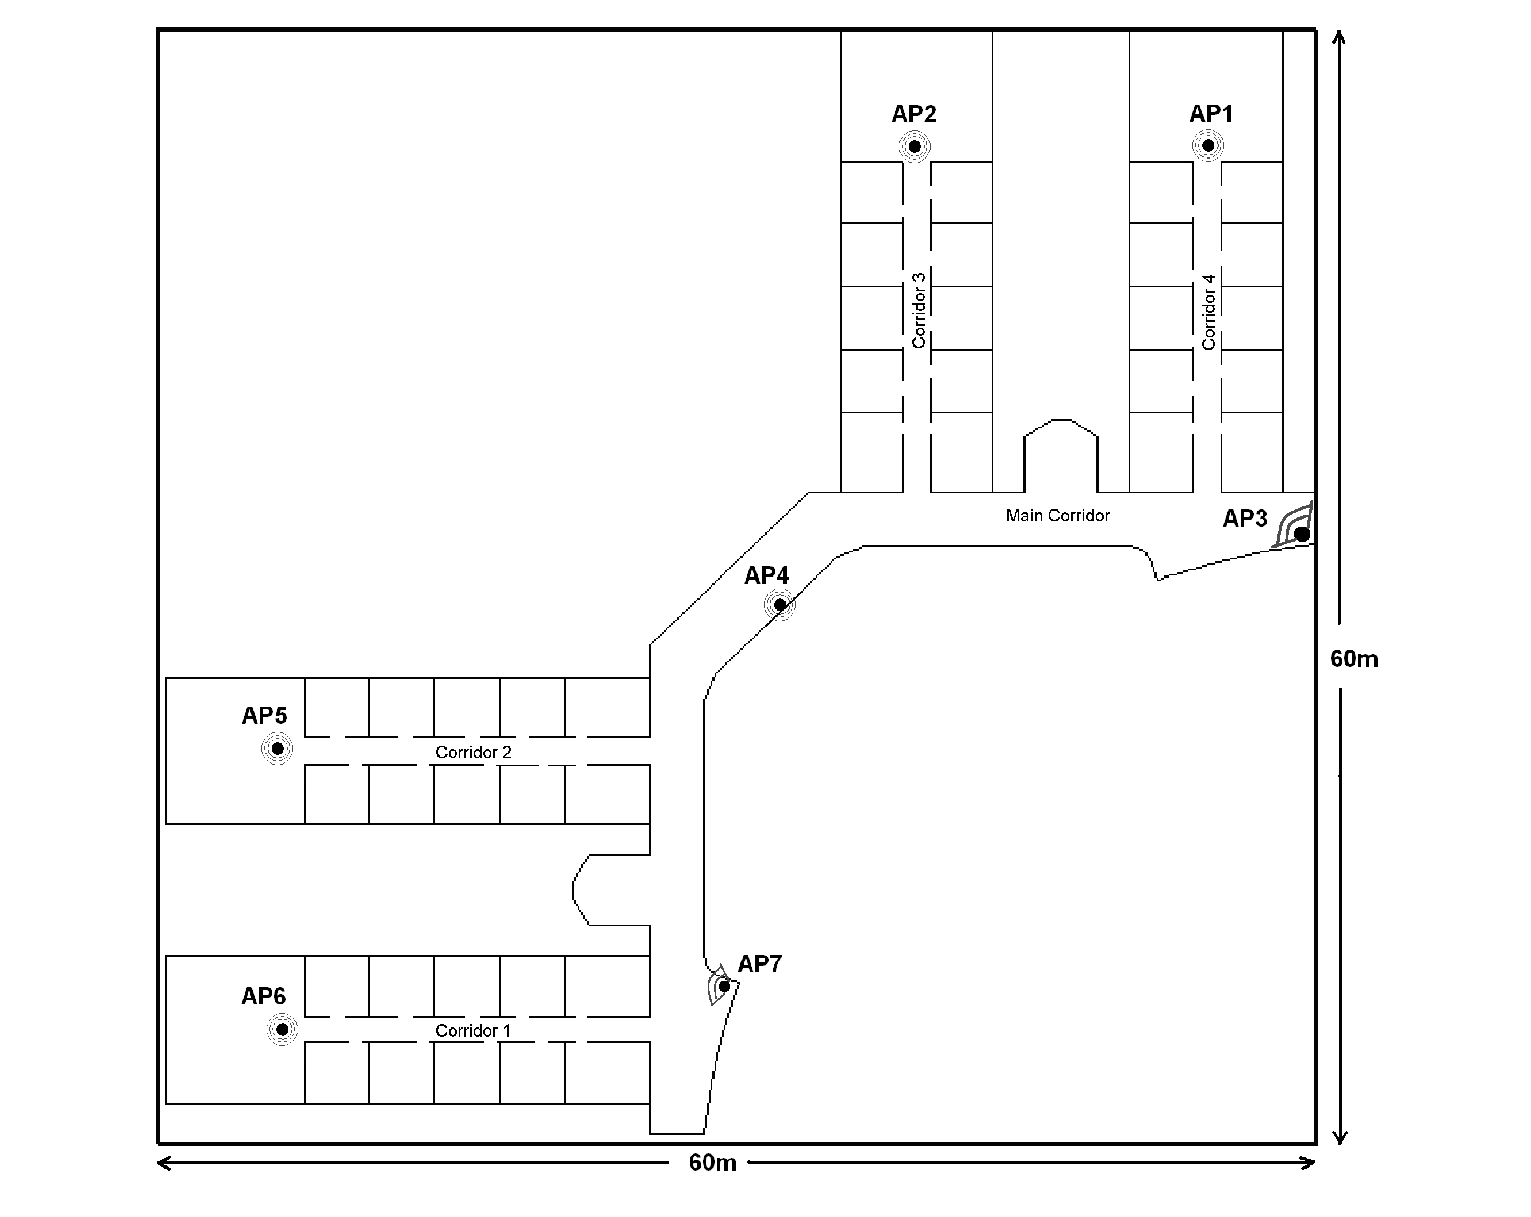
\includegraphics[width=0.55\textwidth]{Figure1}
  \caption{Ejemplo de figura convencional.}
  \label{fig:figura-convencional}
\end{figure}

\subsection{Tabla convencional}
\label{sec:tabla-convencional}

La tabla~\ref{tab:table1} muestra una estructura convencional con título, etiqueta y referencia cruzada.

\begin{table}
  % increase table row spacing, adjust to taste
  \renewcommand{\arraystretch}{1.3}
  \caption{Comparativa.}
  \label{tab:table1}
  \begin{center}
    % Some packages, such as MDW tools, offer better commands for making tables than the plain LaTeX2e tabular which is used here.
    \begin{tabular}{|c|c|c|}
      \hline
      Method & Training Time & Man-Work (\%)\\
      \hline
      Propagation model & $<$ 30 sec & 5\\
      \hline
      Manual & 9 h 30 min & 24\\
      \hline
      Automatic & 2 h & 10 8\\
      \hline
    \end{tabular}
  \end{center}
\end{table}

\subsection{Subfiguras}
\label{sec:subfiguras}

El entorno \texttt{subfigure} permite reunir varias imágenes dentro de una misma figura. La figura~\ref{fig:fig3} contiene dos subfiguras, que también pueden citarse individualmente; por ejemplo, \ref{fig:fig3}.\subref{fig:fig3b}.

% For this to work you need to (in preamble.tex):
% - remove \usepackage{subfig}
% - add \usepackage{caption}
% - add \usepackage{subcaption}
\begin{figure}
  \centering
  \begin{subfigure}[b]{0.3\textwidth}
    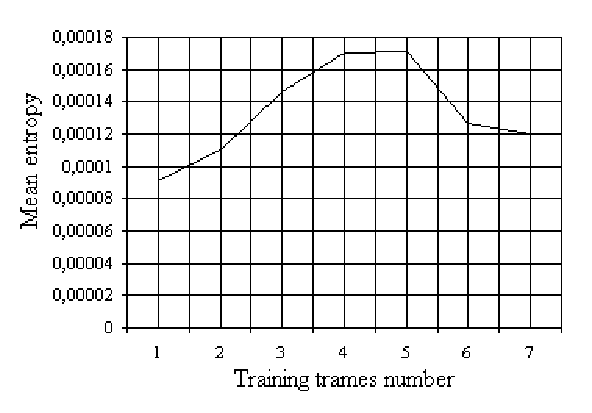
\includegraphics[width=\textwidth]{Figure2}
    \caption{Mean Entropy.}
    \label{fig:fig3a}
  \end{subfigure}%
  ~ %add desired spacing between images, e. g. ~, \quad, \qquad etc.
  % (or a blank line to force the subfigure onto a new line)
  \begin{subfigure}[b]{0.3\textwidth}
    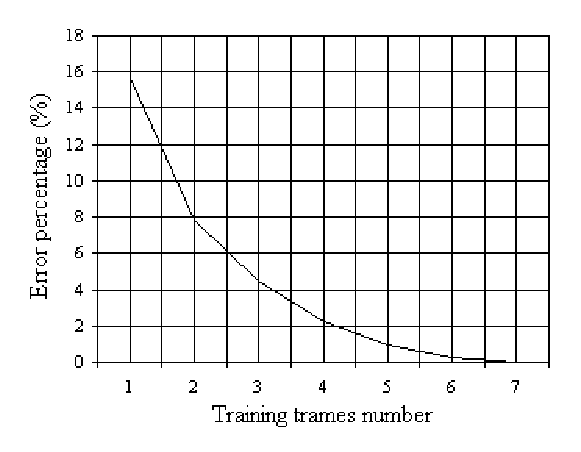
\includegraphics[width=\textwidth]{Figure3}
    \caption{Error Percentage.}
    \label{fig:fig3b}
  \end{subfigure}
  \caption{Optimal trames number in the training data set.}
  \label{fig:fig3}
\end{figure}

Los ejemplos avanzados de figuras y tablas, incluidas las tablas multipágina y apaisadas, las figuras rodeadas por texto y las composiciones con numerosas subfiguras, se encuentran en el capítulo~\ref{cha:ejemplos-avanzados}.


%%% Local Variables:
%%% TeX-master: "../book"
%%% End:


\section{Resumen del capítulo}
\label{sec:resumen-elementos-basicos}

Este capítulo ha mostrado cómo organizar texto, listas y citas, escribir expresiones matemáticas, crear referencias cruzadas y utilizar figuras y tablas habituales. Puedes adaptar estos fragmentos a tu documento y acudir al capítulo~\ref{cha:ejemplos-avanzados} cuando necesites composiciones más elaboradas.

%%% Local Variables:
%%% TeX-master: "../book"
%%% End:

%%%%%%%%%%%%%%%%%%%%%%%%%%%%%%%%%%%%%%%%%%%%%%%%%%%%%%%%%%%%%%%%%%%%%%%%%%%
% Función: ejemplos avanzados de LaTeX.
%
% Uso: modifica este fichero para adaptar el contenido a tu trabajo.
%%%%%%%%%%%%%%%%%%%%%%%%%%%%%%%%%%%%%%%%%%%%%%%%%%%%%%%%%%%%%%%%%%%%%%%%%%%

\chapter{Ejemplos avanzados de composición}
\label{cha:ejemplos-avanzados}

Este capítulo amplía los ejemplos básicos con composiciones que requieren más control sobre la disposición del contenido. Encontrarás distintas combinaciones de figuras y subfiguras, figuras rodeadas por texto y tablas complejas, multipágina, importadas desde LibreOffice o presentadas en horizontal.




\section{Composiciones con subfiguras}
\label{sec:composiciones-subfiguras}

La figura~\ref{fig:LIdiapRoom} muestra otro ejemplo con referencias a las subfiguras desde el pie principal.

\begin{figure}
  \centering
  \begin{subfigure}[b]{0.30\textwidth}
    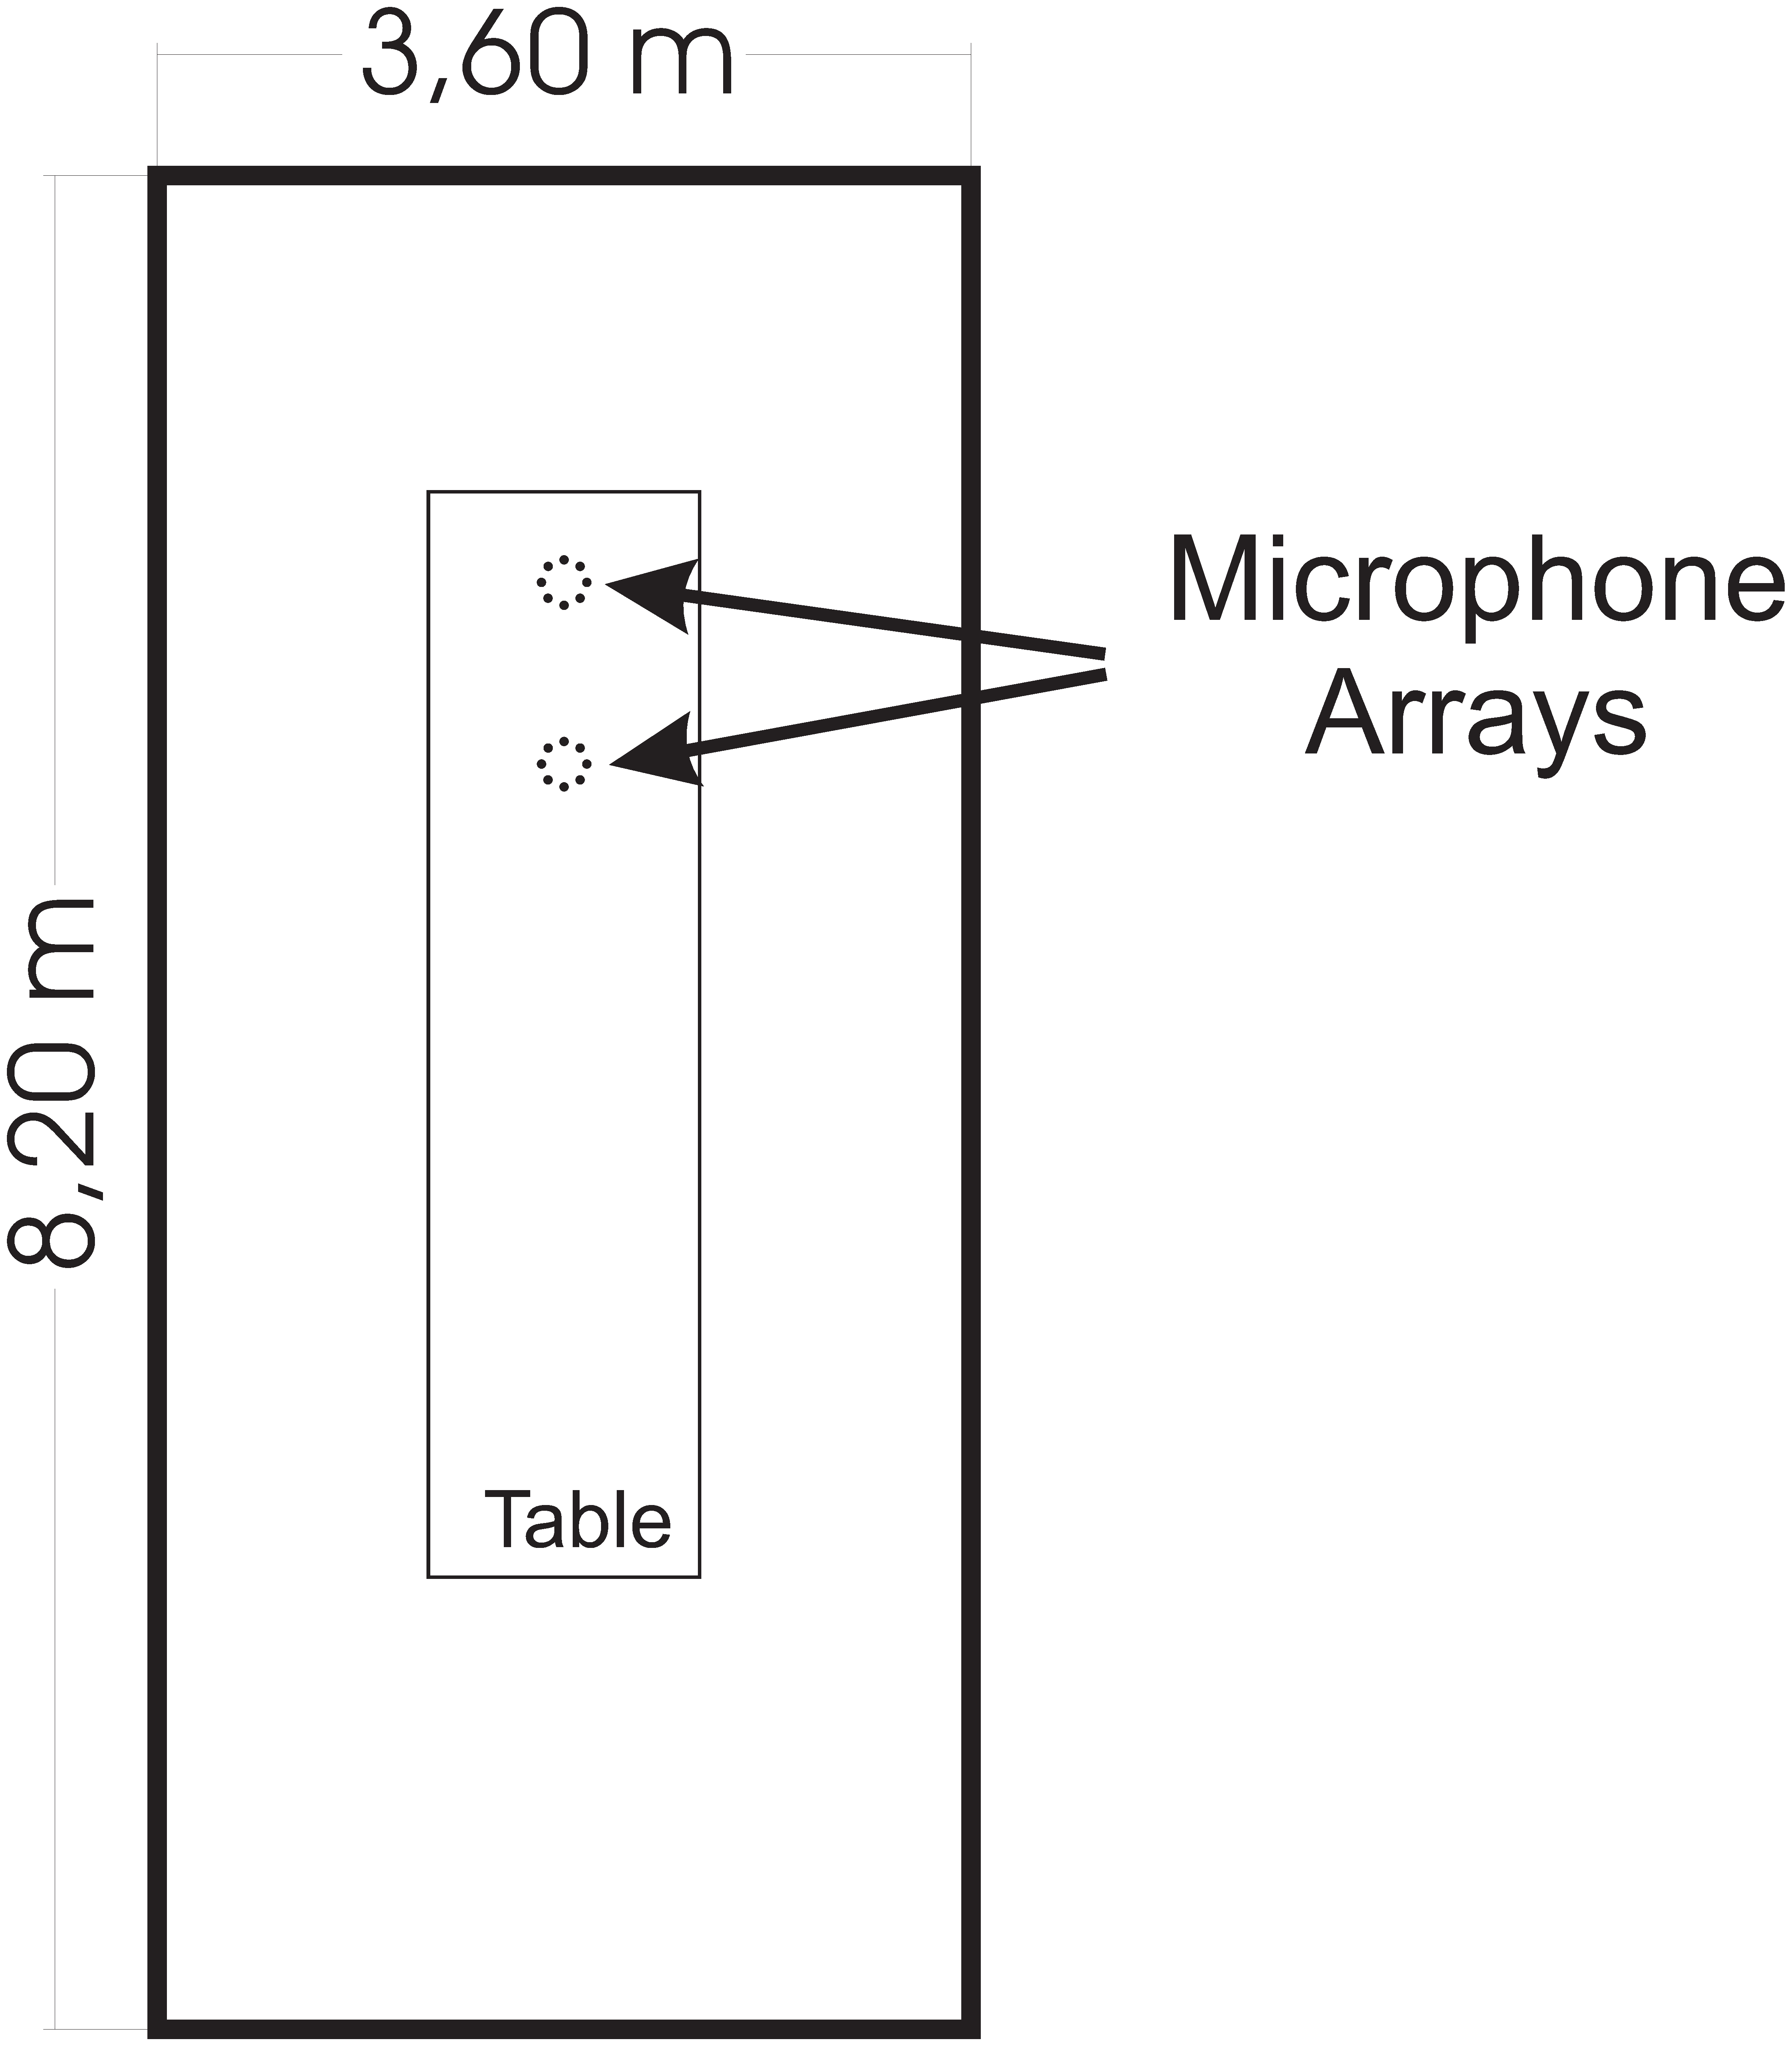
\includegraphics[width=\textwidth]{roomlayout2}
    \caption{}
    \label{fig:RoomLayout}
  \end{subfigure}%
  \qquad \qquad %add desired spacing between images, e. g. ~, \quad, \qquad, \hfill etc.
  % (or a blank line to force the subfigure onto a new line)
  \begin{subfigure}[b]{0.425\textwidth}
    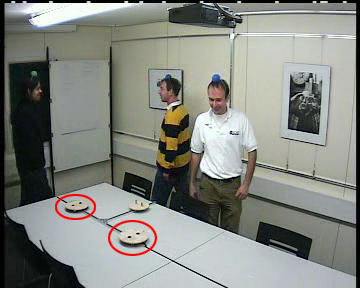
\includegraphics[width=\textwidth]{idiap-seq45-cam2.jpg}
    \caption{}
    \label{fig:RoomPicture}
  \end{subfigure}
  \caption{Idiap Smart Meeting Room for AV16.3 recordings. (\protect\subref{fig:RoomLayout}) Room layout showing the centered table, and the microphones arranged in two circular arrays. (\protect\subref{fig:RoomPicture}) Sample of recorded video frame showing the arrays area. Reproduced from~\cite{velasco2016generative}. %\vspace{-0.3cm}
  }
  \label{fig:LIdiapRoom}
\end{figure}

A continuación incluimos un párrafo de un artículo en el que hacemos referencia a varias figuras y subfiguras (texto tomado de~\cite{velasco2016generative}):

\emph{The IDIAP Meeting Room (shown in figure~\ref{fig:LIdiapRoom}) is a $8.2m \times 3.6m \times 2.4m$ rectangular space containing a centrally located $4.8m \times 1.2m$ rectangular table, on top of which two circular microphone arrays of $10 cm$ radius are located, each of them composed by 8 microphones. The centers of the two arrays are separated by $80 cm$ and the origin of coordinates is located in the middle point between the two arrays. The arrays can be also seen in figures~\ref{fig:simureal_positions}.\subref{fig:Simulated_positions}, ~\ref{fig:simureal_positions}.\subref{fig:real_positions_short}, and ~\ref{fig:simureal_positions}.\subref{fig:real_positions_long}, in which only the relevant section of the room is displayed, each one showing different scenarios that were used in the experiments. A detailed description of the meeting room can be found in~\cite{moore2002}.}

\begin{figure}
  \centering
  \begin{subfigure}[t]{0.3\textwidth}
    
\includegraphics[width=\textwidth]{angular2-short-improved}
    \caption{For validation\\with simulated data.}
    \label{fig:Simulated_positions}
  \end{subfigure}
~%add desired spacing between images, e. g. ~, \quad, \qquad,
  % \hfill etc.
  % (or a blank line to force the subfigure onto a new line)
  \begin{subfigure}[t]{0.3\textwidth}
    
\includegraphics[width=\textwidth]{positions1-short-improved}
    \caption{For validation\\with real data and microphone pairs with $20~cm$ spacing.}
    \label{fig:real_positions_short}
  \end{subfigure}
  ~
  \begin{subfigure}[t]{0.3\textwidth}
    
\includegraphics[width=\textwidth]{positions2-short-improved}
    \caption{For validation\\with real data and microphone pairs with
      $82.46~cm$ spacing.}
    \label{fig:real_positions_long}
  \end{subfigure}
  \caption{Geometrical details for the experiments carried out. Only the
    relevant section of the room is shown, and microphone pairs are
    connected by solid lines. Reproduced from~\cite{velasco2016generative}.}
  \label{fig:simureal_positions}
\end{figure}

En la figura~\ref{fig:Sim_angles} mostramos un ejemplo de varias
figuras organizadas de forma un poco más complejo.

\begin{figure}
  \centering
  \begin{subfigure}[b]{0.3\textwidth}
    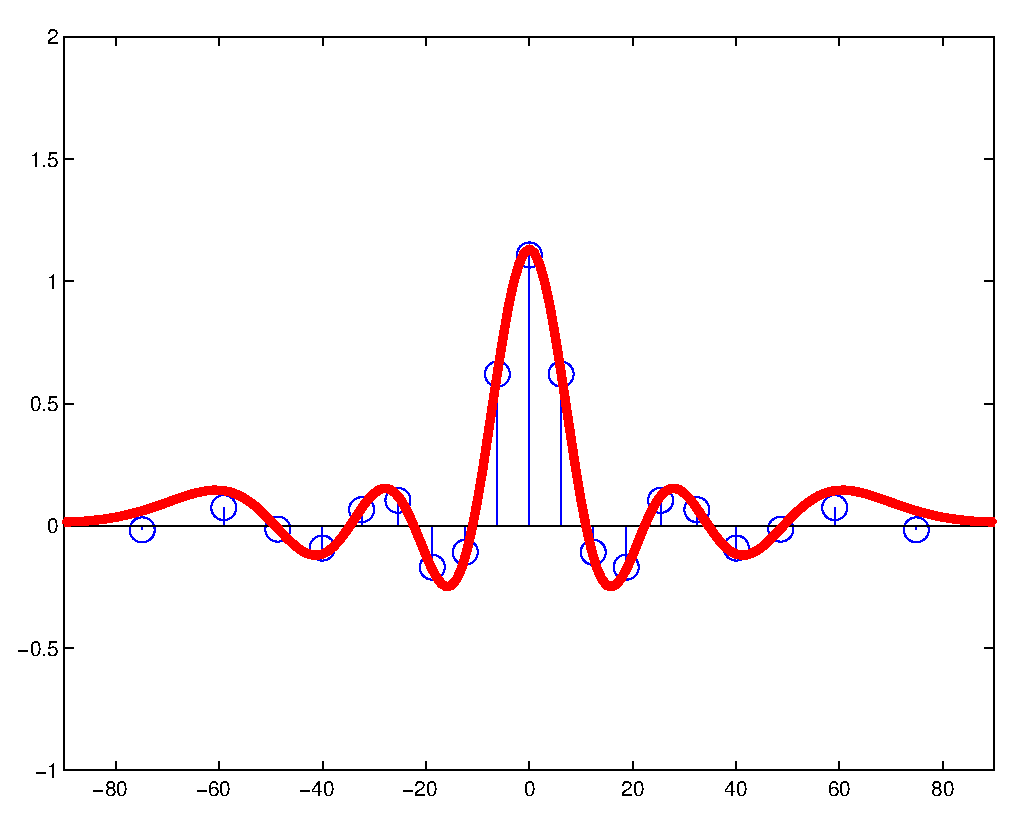
\includegraphics[width=\textwidth]{Sim_seg025_ang090}
    \caption{$0^{\circ}$}
    \label{fig:Sim_ang090}
  \end{subfigure}
  % add desired spacing between images, e. g. ~, \quad, \qquad etc.
  % (or a blank line to force the subfigure onto a new line)

  \begin{subfigure}[b]{0.3\textwidth}
    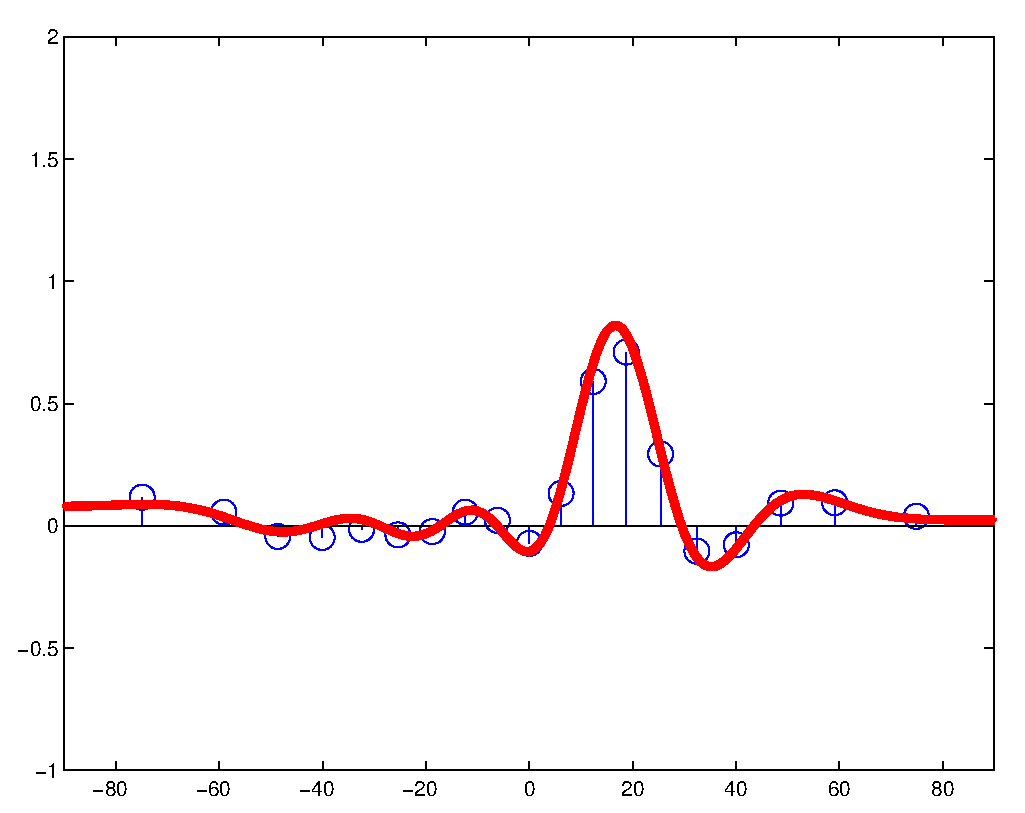
\includegraphics[width=\textwidth]{Sim_seg025_ang108}
    \caption{$18^{\circ}$}
    \label{fig:Sim_ang108}
  \end{subfigure}
  % add desired spacing between images, e. g. ~, \quad, \qquad etc.
  % (or a blank line to force the subfigure onto a new line)
  \begin{subfigure}[b]{0.3\textwidth}
    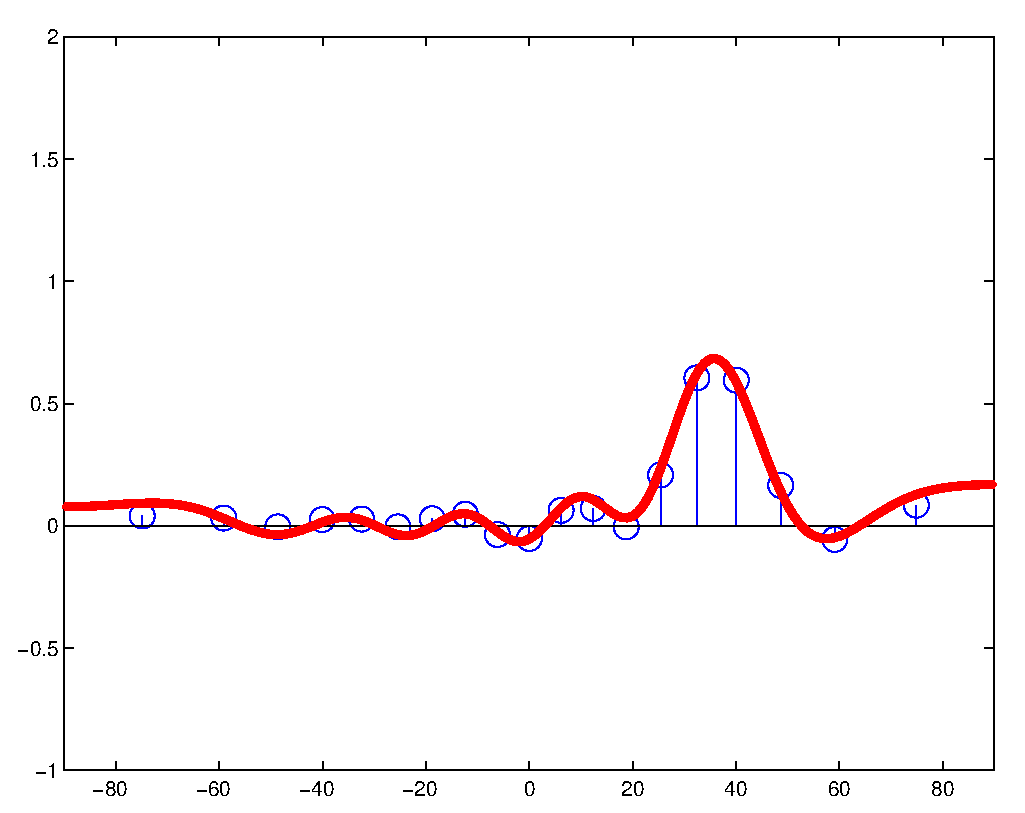
\includegraphics[width=\textwidth]{Sim_seg025_ang126}
    \caption{$36^{\circ}$}
    \label{fig:Sim_ang126}
  \end{subfigure}
  % add desired spacing between images, e. g. ~, \quad, \qquad etc.
  % (or a blank line to force the subfigure onto a new line)
  \begin{subfigure}[b]{0.3\textwidth}
    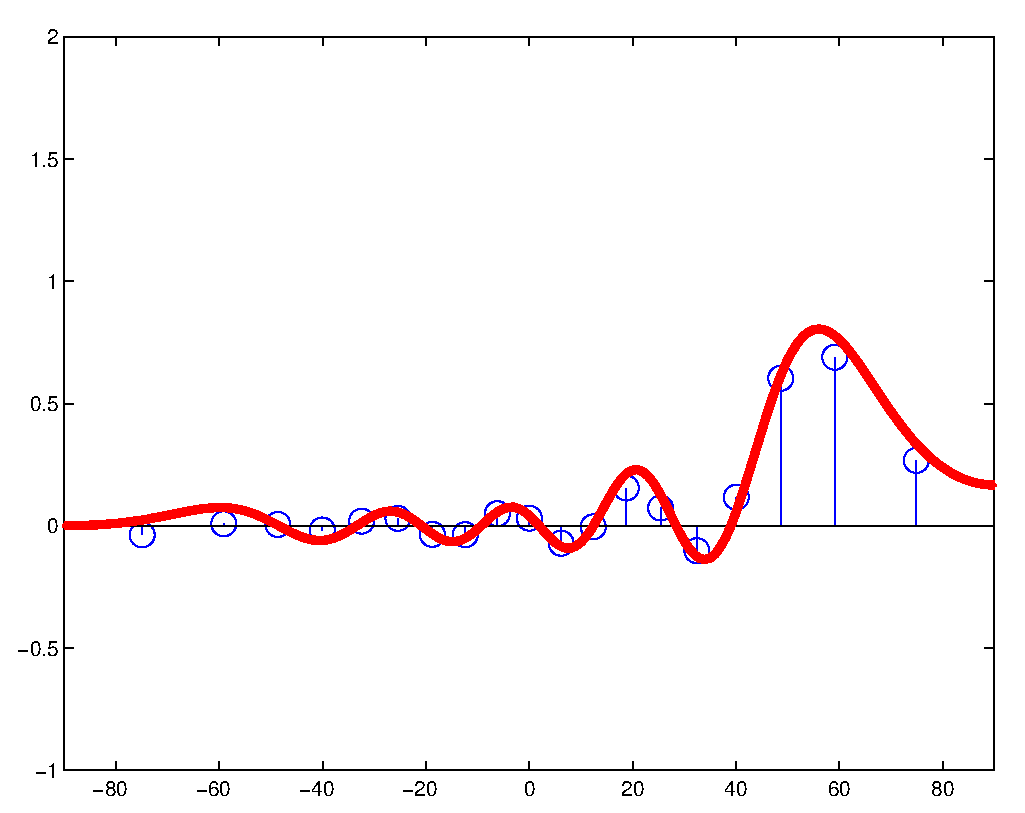
\includegraphics[width=\textwidth]{Sim_seg025_ang144}
    \caption{$54^{\circ}$}
    \label{fig:Sim_ang144}
  \end{subfigure}
  % add desired spacing between images, e. g. ~, \quad, \qquad etc.
  % (or a blank line to force the subfigure onto a new line)

  \begin{subfigure}[b]{0.3\textwidth}
    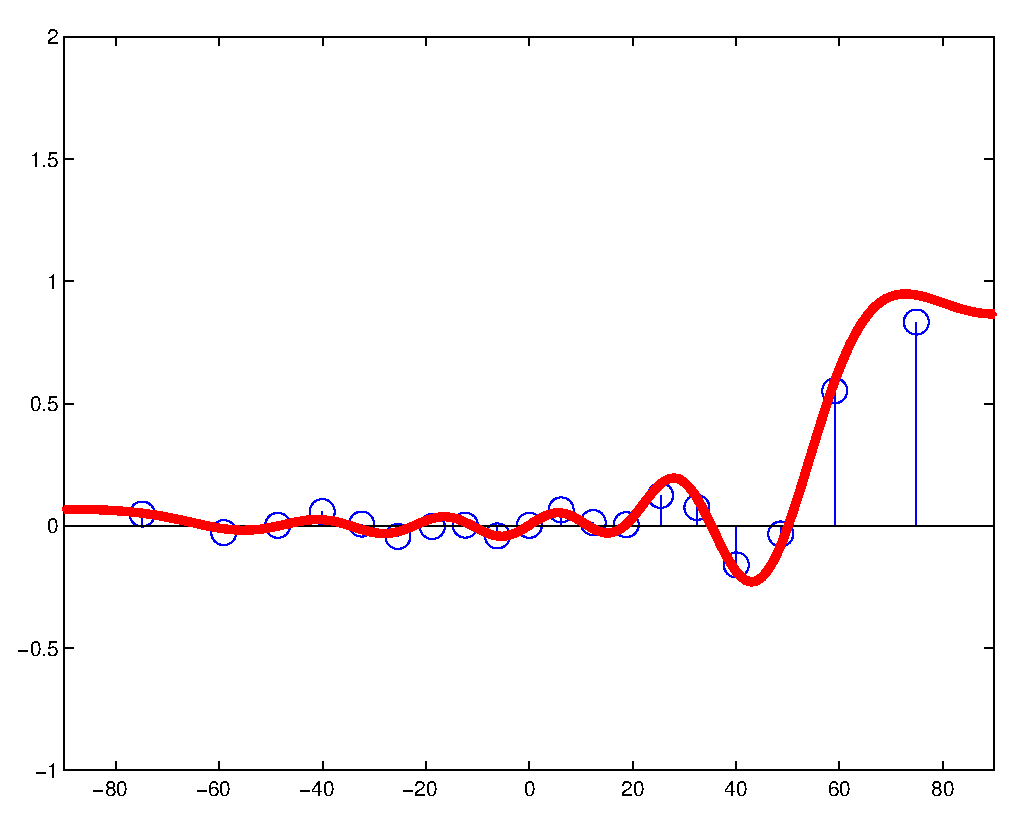
\includegraphics[width=\textwidth]{Sim_seg025_ang162}
    \caption{$72^{\circ}$}
    \label{fig:Sim_ang162}
  \end{subfigure}

  \caption{Comparison between the steered power response generated by the model (solid line) and that calculated using simulated waveforms in the AV16.3 environment (stems). Results for the speaker in given angles and the array steered from -90º to +90º are shown. Reproduced from~\cite{velasco2016generative}.}
  \label{fig:Sim_angles}
\end{figure}

\section{Figuras definidas en ficheros independientes}
\label{sec:figuras-ficheros-independientes}

También es posible incluir el código de una figura en un fichero \texttt{.tex} independiente (para hacer más legible el código del documento principal). El siguiente ejemplo lo muestra, incluyendo el texto en inglés del documento original (tomado de~\cite{velasco2016generative}):

\emph{Figure~\ref{fig:SRPvsPatternSelected} includes the results of the comparison, for several speaker positions (1, 2, 4, 6, 8 and 16, emphasized in figure~\ref{fig:simureal_positions}.\subref{fig:real_positions_short}), and selected to provide different acoustic situations, both in terms of distance and angular position with respect to the arrays. All the graphics show the acoustic power map (predicted or calculated) for a regular two-dimensional grid of $10~cm$. The plot is provided from a top view of the room, spanning the full plan at a height of $61~cm$ above the microphone arrays (this height was the ground truth one for sequence 01). For each speaker position shown, three graphics are plotted:}

\begin{itemize}
  \item \emph{The graphics on the left show the SRP-PHAT acoustic power maps generated by the proposed model (for example, the left graphic in figure~\ref{fig:SRPvsPatternSelected}.\subref{fig:SRPvsModel_Fo1500_position1} for position 1).}
  \item \emph{The graphics in the middle show the real SRP-PHAT acoustic power maps calculated using the real acoustic waveforms (for example, the middle graphic in figure~\ref{fig:SRPvsPatternSelected}.\subref{fig:SRPvsModel_Fo1500_position1} for position 1), for a single selected frame.}
  \item \emph{The graphics on the right show the average real SRP-PHAT acoustic power maps, averaging for all the frames in which the user was in the given position (for example, the right graphic in figure~\ref{fig:SRPvsPatternSelected}.\subref{fig:SRPvsModel_Fo1500_position1} for position 1).}
\end{itemize}

\emph{The green point represents the real (ground truth) speaker position, and the black dots represent the positions of the four microphones used. The hyperbolic shapes found in the figure are consistent with the fact that the place of points with equal acoustic power value, for a given microphone pair, is a hyperbola (in our two-dimensional case, being a hyperboloid of revolution in the three-dimensional case).}

\emph{From figure~\ref{fig:SRPvsPatternSelected}, it can clearly be seen that, again, the predictions closely match the results with real data for the different acoustic conditions, even when the simulations are using fixed and frequency independent average reflection coefficients, and that the acoustic model is based on the simplistic image method model.}

%%%%%%%%%%%%%%%%%%%%%%%%%%%%%%%%%%%%%%%%%%%%%%%%%%%%%%%%%%%%%%%%%%%%%%%%%%%
% Purpose: sample figure comparing localization maps.
%
% Usage: edit this example as needed; include it from a chapter.
% It is not compiled separately.
%%%%%%%%%%%%%%%%%%%%%%%%%%%%%%%%%%%%%%%%%%%%%%%%%%%%%%%%%%%%%%%%%%%%%%%%%%%

\begin{figure}
  \centering
  \begin{subfigure}[t]{0.47\textwidth}
    \begin{minipage}[t]{\textwidth}
      \begin{subfigure}[t]{0.3\textwidth}
        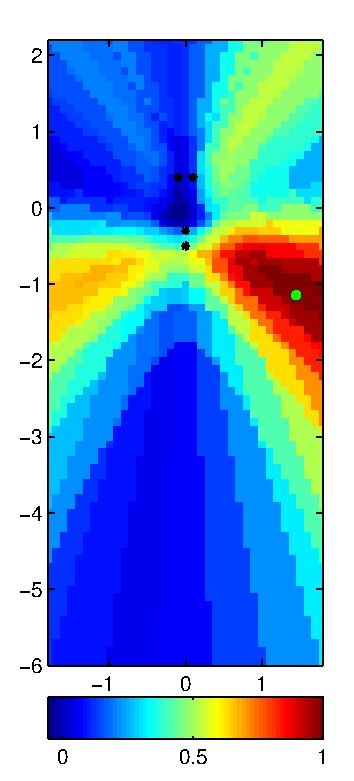
\includegraphics[width=\textwidth]{Pattern_Fo1500_pos01}
        %\caption{SRP Model for pos. 1}
        \label{fig:Pattern_Fo1500_pos01}
      \end{subfigure}
      % ~ %add desired spacing between images, e. g. ~, \quad, \qquad,
      % \hfill etc.
      % (or a blank line to force the subfigure onto a new line)
      \begin{subfigure}[t]{0.3\textwidth}
        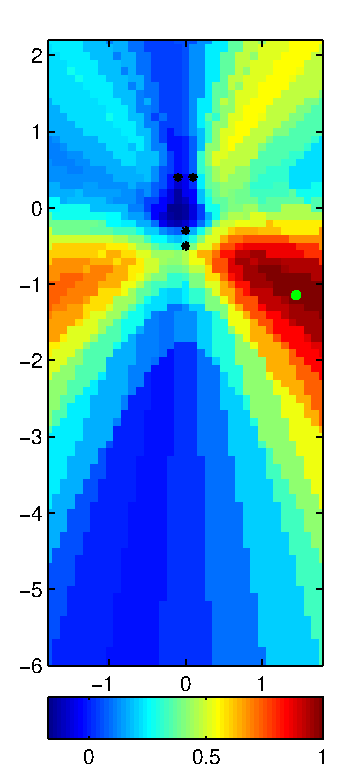
\includegraphics[width=\textwidth]{SRP_Fo1500_frame003_pos01}
        % \caption{Real SRP for pos.  1}
        \label{fig:SRP_Fo1500_pos01}
      \end{subfigure}
      % ~ %add desired spacing between images, e. g. ~, \quad, \qquad,
      % \hfill etc.
      % (or a blank line to force the subfigure onto a new line)
      \begin{subfigure}[t]{0.3\textwidth}
        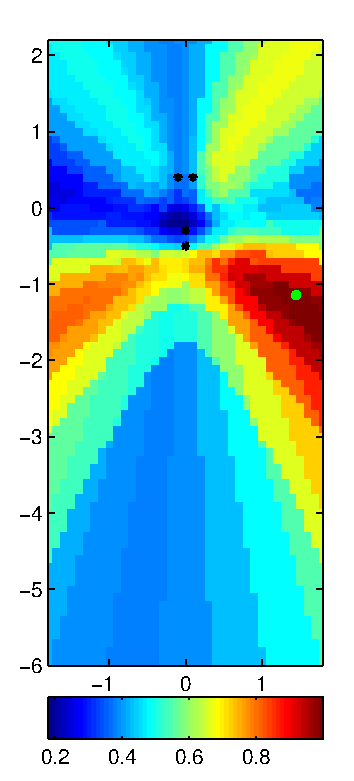
\includegraphics[width=\textwidth]{SRP_Fo1500_mean_pos01}
        % \caption{Avg. SRP for pos. 1}
        \label{fig:SRP_Fo1500_mean_pos01}
      \end{subfigure}
      \vspace{\verticalSpacingSRPMaps}
      \caption{\centering For position 1}
      \label{fig:SRPvsModel_Fo1500_position1}
      \vspace{0.25cm}
    \end{minipage}
  \end{subfigure}
  ~% \quad % between 1 and 2 %add desired spacing between images, e. g. ~, \quad, \qquad,
  % \hfill etc.
  % (or a blank line to force the subfigure onto a new line)
  \begin{subfigure}[t]{0.47\textwidth}
    \begin{minipage}[t]{\textwidth}
      \begin{subfigure}[t]{0.3\textwidth}
        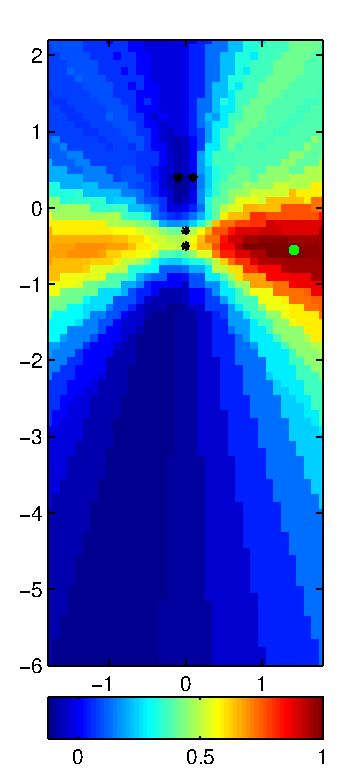
\includegraphics[width=\textwidth]{Pattern_Fo1500_pos02}
        % \caption{SRP Model for pos. 2}
        \label{fig:Pattern_Fo1500_pos02}
      \end{subfigure}
      % ~ %add desired spacing between images, e. g. ~, \quad, \qquad,
      % \hfill etc.
      % (or a blank line to force the subfigure onto a new line)
      \begin{subfigure}[t]{0.3\textwidth}
        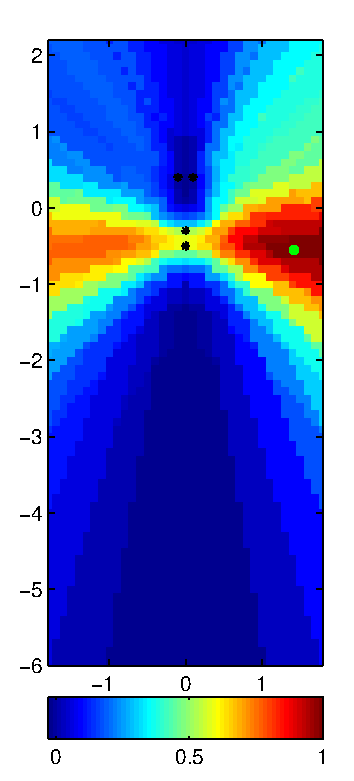
\includegraphics[width=\textwidth]{SRP_Fo1500_frame161_pos02}
        % \caption{Real SRP for pos.  2\\}
        \label{fig:SRP_pos02}
      \end{subfigure}
      % ~ %add desired spacing between images, e. g. ~, \quad, \qquad,
      % \hfill etc.
      % (or a blank line to force the subfigure onto a new line)
      \begin{subfigure}[t]{0.3\textwidth}
        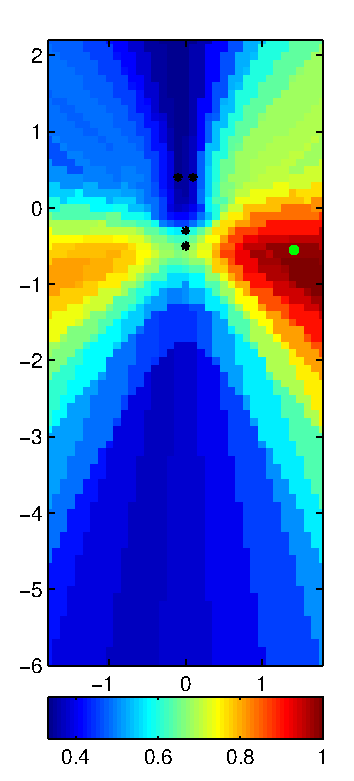
\includegraphics[width=\textwidth]{SRP_Fo1500_mean_pos02}
        % \caption{Avg. SRP for pos. 2}
        \label{fig:SRP_Fo1500_mean_pos02}
      \end{subfigure}
      \vspace{\verticalSpacingSRPMaps}
      \caption{\centering For position 2}
      \vspace{0.25cm}
    \end{minipage}
  \end{subfigure}

  \begin{subfigure}[t]{0.47\textwidth}
    \begin{minipage}[t]{\textwidth}
      \begin{subfigure}[t]{0.3\textwidth}
        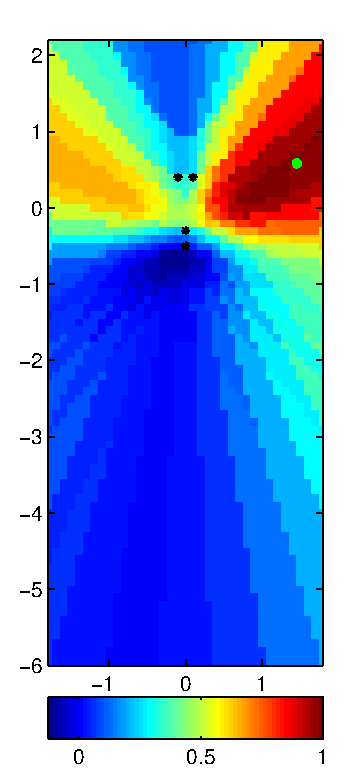
\includegraphics[width=\textwidth]{Pattern_Fo1500_pos04}
        % \caption{SRP Model for pos. 4}
        \label{fig:Pattern_Fo1500_pos04}
      \end{subfigure}
      % ~ %add desired spacing between images, e. g. ~, \quad, \qquad,
      % \hfill etc.
      % (or a blank line to force the subfigure onto a new line)
      \begin{subfigure}[t]{0.3\textwidth}
        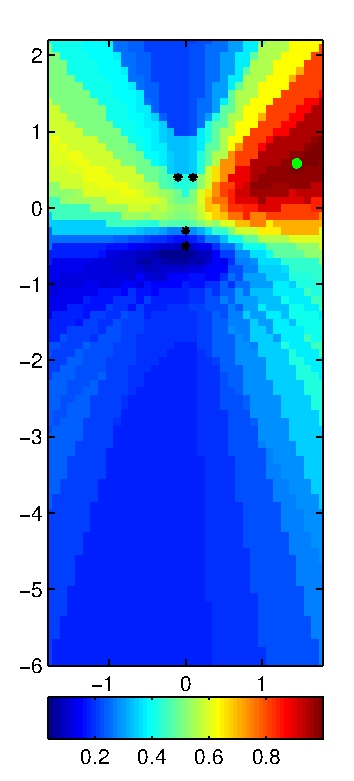
\includegraphics[width=\textwidth]{SRP_Fo1500_frame464_pos04}
        % \caption{Real SRP for pos.  4\\}
        \label{fig:SRP_pos04}
      \end{subfigure}
      % ~ %add desired spacing between images, e. g. ~, \quad, \qquad,
      % \hfill etc.
      % (or a blank line to force the subfigure onto a new line)
      \begin{subfigure}[t]{0.3\textwidth}
        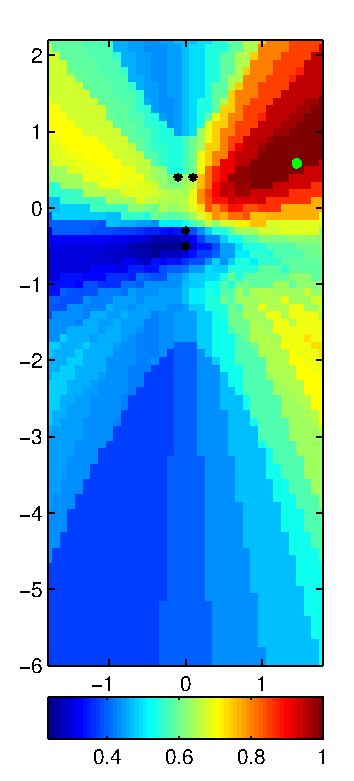
\includegraphics[width=\textwidth]{SRP_Fo1500_mean_pos04}
        % \caption{Avg. SRP for pos. 4}
        \label{fig:SRP_Fo1500_mean_pos04}
      \end{subfigure}
      \vspace{\verticalSpacingSRPMaps}
      \caption{\centering For position 4}
      \vspace{0.25cm}
    \end{minipage}
  \end{subfigure}
  ~%  \qquad % between 4 and 6 %add desired spacing between images, e. g. ~, \quad, \qquad,
  % \hfill etc.
  % (or a blank line to force the subfigure onto a new line)
  \begin{subfigure}[t]{0.47\textwidth}
    \begin{minipage}[t]{\textwidth}
      \begin{subfigure}[t]{0.3\textwidth}
        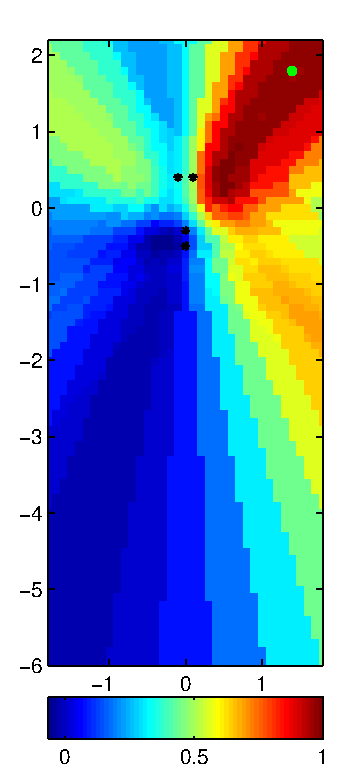
\includegraphics[width=\textwidth]{Pattern_Fo1500_pos06}
        % \caption{SRP Model for pos. 6}
        \label{fig:Pattern_Fo1500_pos06}
      \end{subfigure}
      % ~ %add desired spacing between images, e. g. ~, \quad, \qquad,
      % \hfill etc.
      % (or a blank line to force the subfigure onto a new line)
      \begin{subfigure}[t]{0.3\textwidth}
        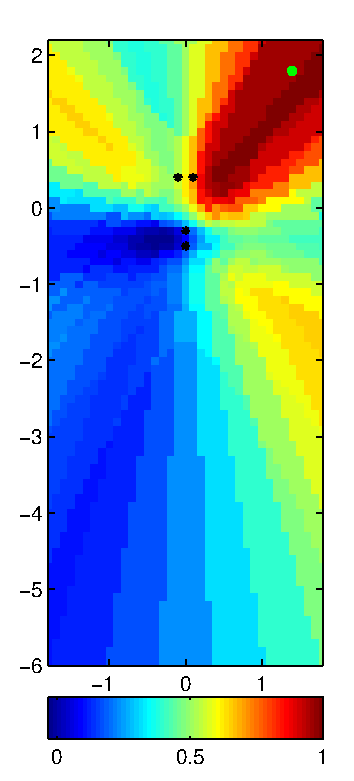
\includegraphics[width=\textwidth]{SRP_Fo1500_frame809_pos06}
        % \caption{Real SRP for pos.  6\\}
        \label{fig:SRP_pos06}
      \end{subfigure}
      % ~ %add desired spacing between images, e. g. ~, \quad, \qquad,
      % \hfill etc.
      % (or a blank line to force the subfigure onto a new line)
      \begin{subfigure}[t]{0.3\textwidth}
        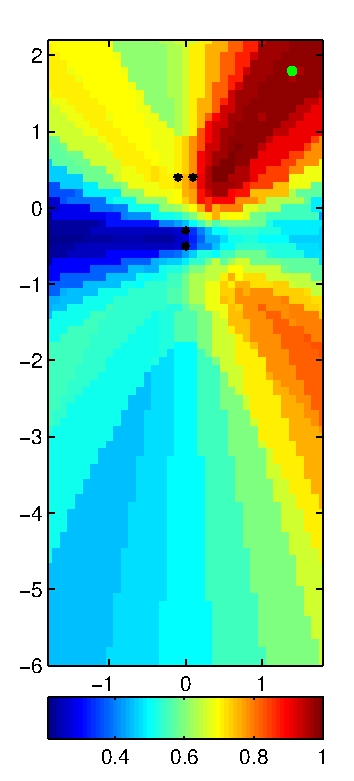
\includegraphics[width=\textwidth]{SRP_Fo1500_mean_pos06}
        % \caption{Avg. SRP for pos. 6}
        \label{fig:SRP_Fo1500_mean_pos06}
      \end{subfigure}
      \vspace{\verticalSpacingSRPMaps}
      \caption{\centering For position 6}
      \vspace{0.25cm}
    \end{minipage}
  \end{subfigure}

  \begin{subfigure}[t]{0.47\textwidth}
    \begin{minipage}[t]{\textwidth}
      \begin{subfigure}[t]{0.3\textwidth}
        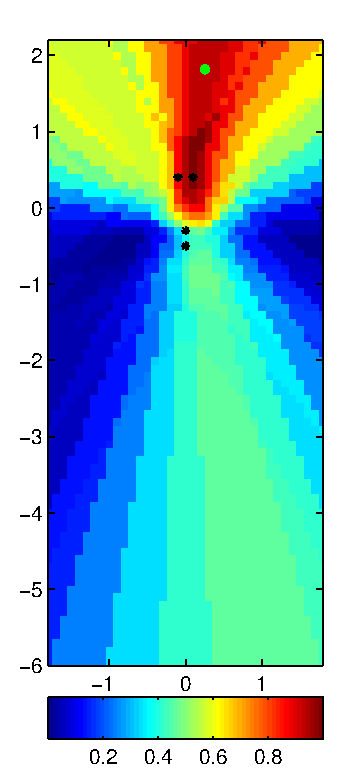
\includegraphics[width=\textwidth]{Pattern_Fo1500_pos08}
        % \caption{SRP Model for pos. 8}
        \label{fig:Pattern_Fo1500_pos08}
      \end{subfigure}
      % ~ %add desired spacing between images, e. g. ~, \quad, \qquad,
      % \hfill etc.
      % (or a blank line to force the subfigure onto a new line)
      \begin{subfigure}[t]{0.3\textwidth}
        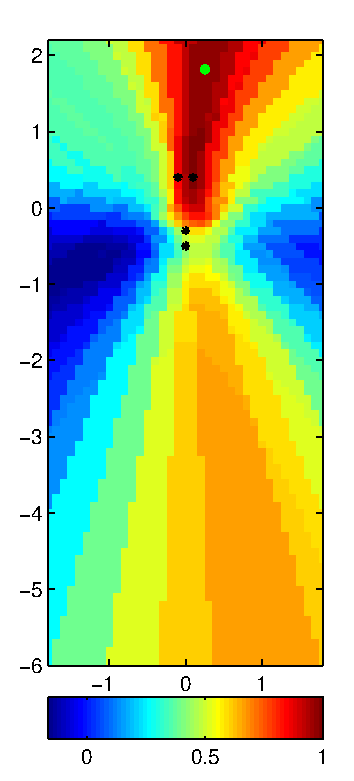
\includegraphics[width=\textwidth]{SRP_Fo1500_frame1127_pos08}
        % \caption{Real SRP for pos.  8\\}
        \label{fig:SRP_pos08}
      \end{subfigure}
      % ~ %add desired spacing between images, e. g. ~, \quad, \qquad,
      % \hfill etc.
      % (or a blank line to force the subfigure onto a new line)
      \begin{subfigure}[t]{0.3\textwidth}
        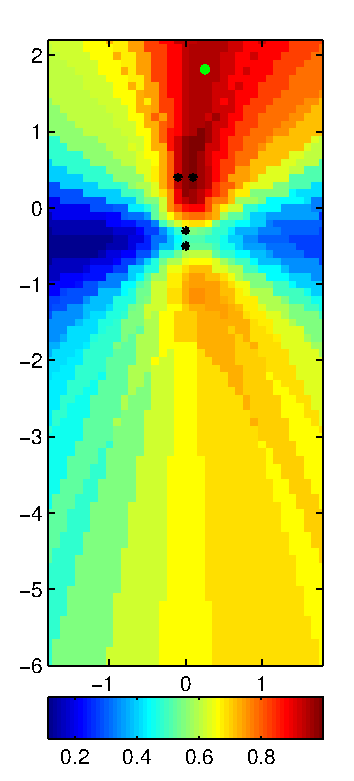
\includegraphics[width=\textwidth]{SRP_Fo1500_mean_pos08}
        % \caption{Avg. SRP for pos. 8}
        \label{fig:SRP_Fo1500_mean_pos08}
      \end{subfigure}
      \vspace{\verticalSpacingSRPMaps}
      \caption{\centering For position 8}
      \vspace{0.25cm}
    \end{minipage}
  \end{subfigure}
  ~%  \qquad % between 8 and 16 %add desired spacing between images, e. g. ~, \quad, \qquad,
  % \hfill etc.
  % (or a blank line to force the subfigure onto a new line)
  \begin{subfigure}[t]{0.47\textwidth}
    \begin{minipage}[t]{\textwidth}
      \begin{subfigure}[t]{0.3\textwidth}
        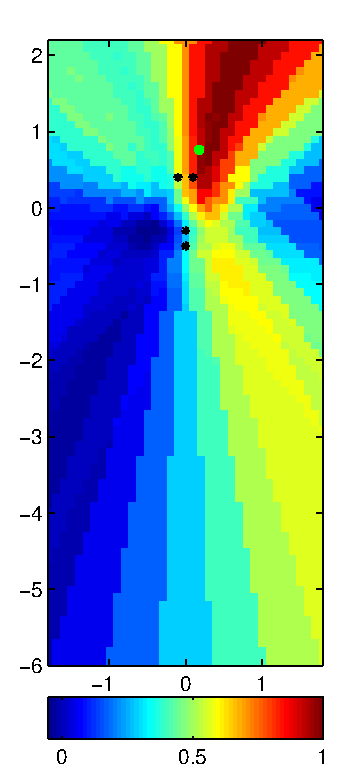
\includegraphics[width=\textwidth]{Pattern_Fo1500_pos16}
        % \caption{SRP Model for pos. 16}
        \label{fig:Pattern_Fo1500_pos16}
      \end{subfigure}
      % ~ %add desired spacing between images, e. g. ~, \quad, \qquad,
      % \hfill etc.
      % (or a blank line to force the subfigure onto a new line)
      \begin{subfigure}[t]{0.3\textwidth}
        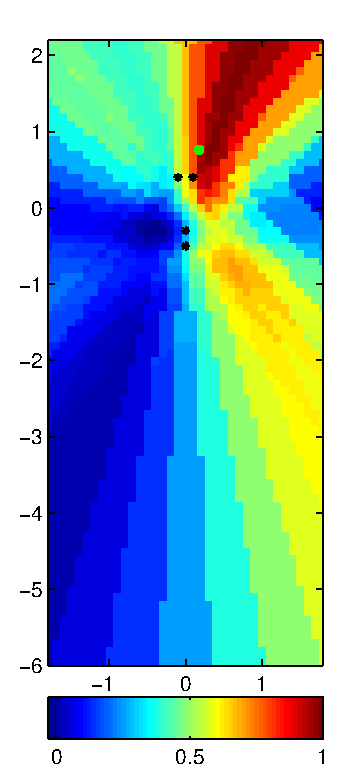
\includegraphics[width=\textwidth]{SRP_Fo1500_frame2518_pos16}
        % \caption{Real SRP for pos. 16\\}
        \label{fig:SRP_pos16}
      \end{subfigure}
      % ~ %add desired spacing between images, e. g. ~, \quad, \qquad,
      % \hfill etc.
      % (or a blank line to force the subfigure onto a new line)
      \begin{subfigure}[t]{0.3\textwidth}
        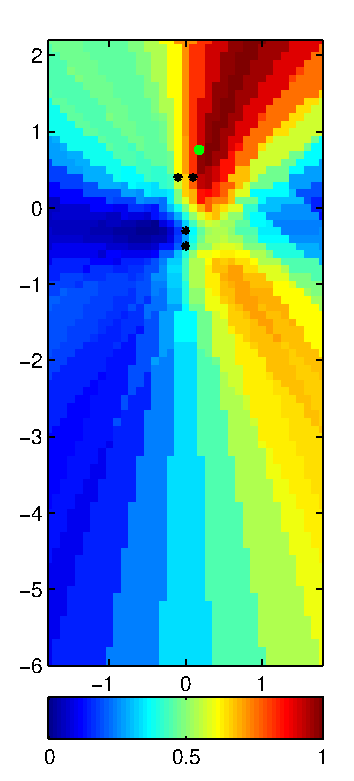
\includegraphics[width=\textwidth]{SRP_Fo1500_mean_pos16}
        % \caption{Avg. SRP for pos. 16}
        \label{fig:SRP_Fo1500_mean_pos16}
      \end{subfigure}
      \vspace{\verticalSpacingSRPMaps}
      \caption{\centering For position 16}
      \vspace{0.25cm}
    \end{minipage}
  \end{subfigure}
  \caption{Comparison between the SRP-PHAT map predicted by the model (left graphics), the real SRP-PHAT map (middle graphics), and the average (real) SRP-PHAT map (right graphics), for several speaker positions ($f_0=1.5~KHz$). See figure~~\ref{fig:simureal_positions}.\subref{fig:real_positions_short} for geometrical references. Reproduced from~\cite{velasco2016generative}.}
  \label{fig:SRPvsPatternSelected}
\end{figure}
 

\section{Figuras rodeadas por texto}
\label{sec:figuras-rodeadas-texto}

\begin{wrapfigure}{r}{0.5\textwidth} 
\vspace{-20pt}
  \begin{center}
    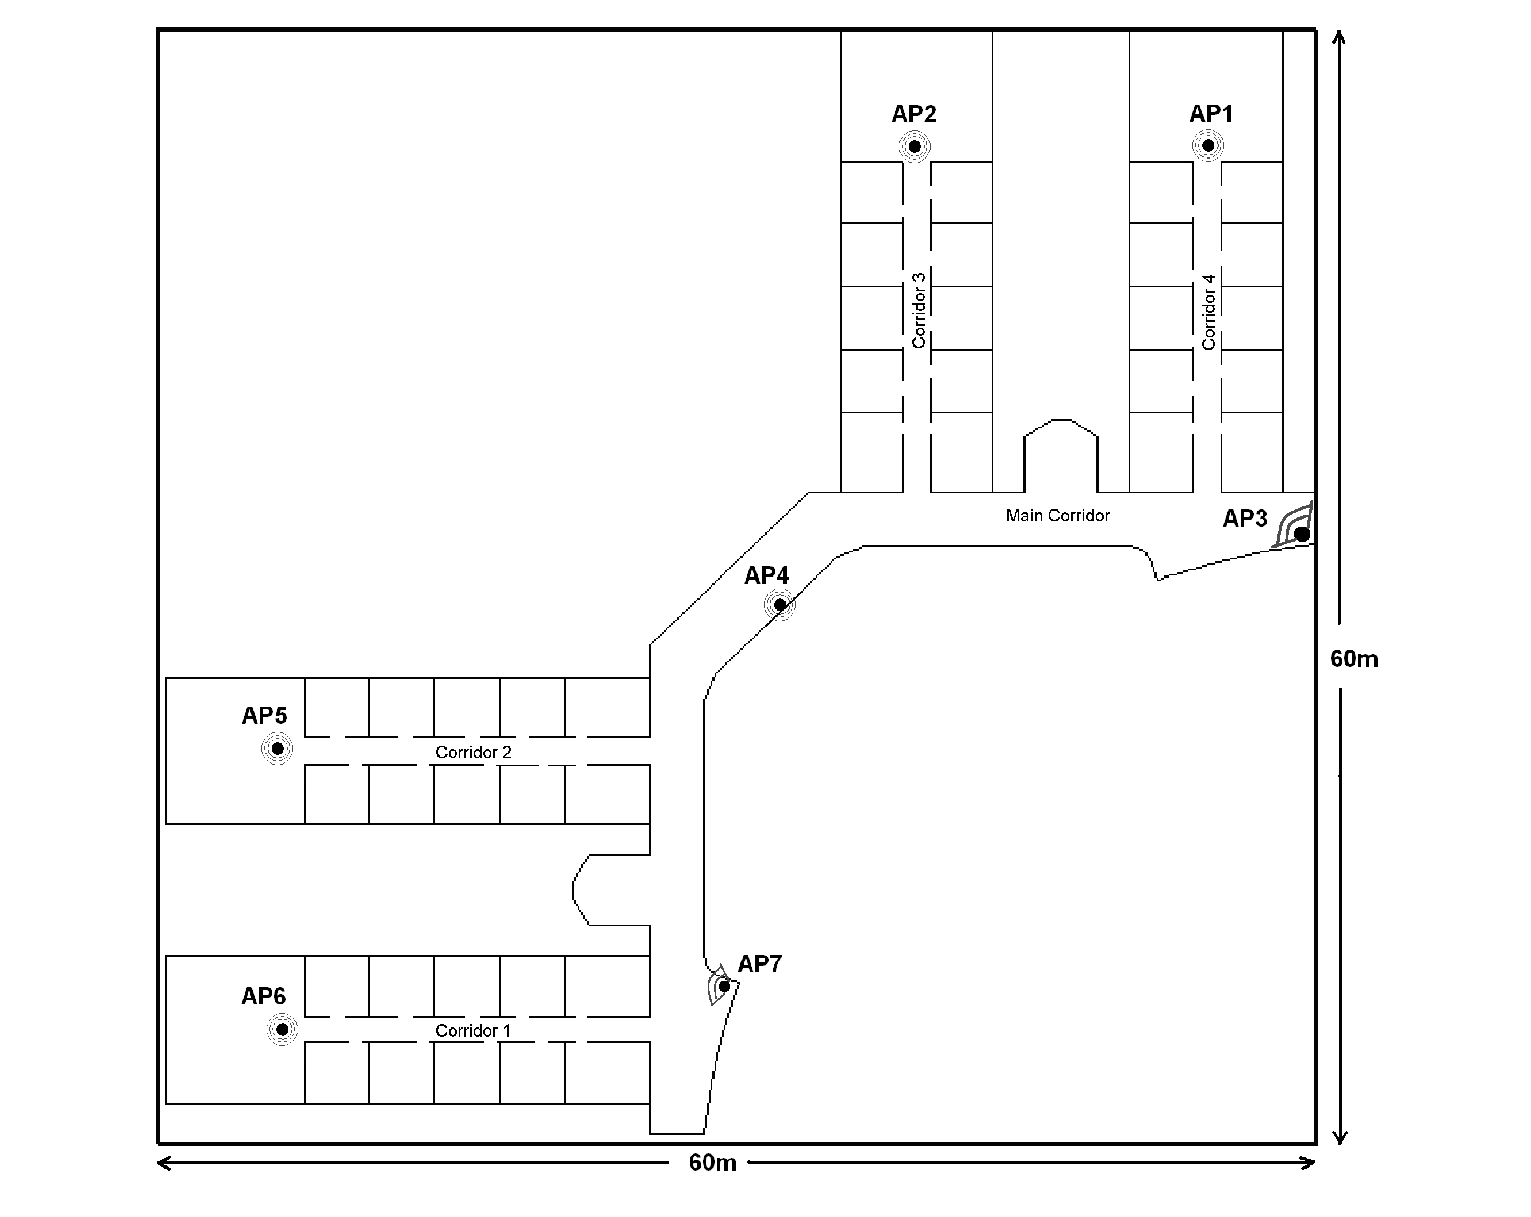
\includegraphics[width=0.4\textwidth]{Figure1}
    \caption{Ejemplo de figura con wrapfigure.}
    \label{fig:wrapfigure1}
  \end{center}
  \vspace{-20pt}
  \vspace{1pt}
\end{wrapfigure} 

Otra posibilidad es utilizar el entorno \texttt{wrapfig} para hacer que el texto bordee a las figuras, como en la figura~\ref{fig:wrapfigure1}. Añadimos unas líneas de Lorem ipsum para que puedas ver el resultado.

\lipsum[1-1]

% \lipsum[1-4]
% \begin{wrapfigure}{R}{5cm}
% \centering
% \rule{3cm}{7cm}
% \end{wrapfigure}
% \lipsum[1-6]


\section{Tablas complejas}
\label{sec:tablas-complejas}

La generación de tablas complejas es, en general, una pesadilla. Para aliviar esa dificultad puedes utilizar inicialmente herramientas externas como \href{https://www.tablesgenerator.com/}{Tables Generator}. El ejemplo de la tabla~\ref{tab:MethodSummaryCAV3D} está tomado de~\cite{Sanabria2026Landmark} y fue generado inicialmente con esa aplicación (cuando la uses, no olvides guardar el fichero \texttt{.tgn} correspondiente, para que puedas volver a editarlo en el futuro).

En ese ejemplo de la tabla~\ref{tab:MethodSummaryCAV3D} puedes ver agrupaciones de celdas y alineamientos variados, así como cambios en el color de fondo de algunas celdas. También puedes ver el uso de comandos predefinidos que facilitan la consistencia de los documentos y permiten cambios rápidos de formato. Por ejemplo, fíjate en \texttt{\\DeltaPoseAVT\{\}} que se traduce en \DeltaPoseAVT{} (todos esos comandos los encontrarás en \texttt{Config/myconfig.tex}, y ahí mismo puedes añadir los que necesite tu documento).

% Please add the following required packages to your document preamble:
% \usepackage{multirow}
% \usepackage[table,xcdraw]{xcolor}
% Beamer presentation requires \usepackage{colortbl} instead of \usepackage[table,xcdraw]{xcolor}
\begin{table}[h]
  \centering
  \resizebox{\textwidth}{!}{
    \begin{tabular}{cl|ccc|ccc|c}
      \cline{3-8}
      & \multicolumn{1}{c|}{}                                 & \multicolumn{3}{c|}{2D}                                                                                                                                                                                                                   & \multicolumn{3}{c|}{3D}                                                                                                                                                                                                                   &                                                                                      \\ \cline{1-9}
            \multicolumn{1}{|c|}{\textbf{Method}}
      & \multicolumn{1}{c|}{\textbf{Data}}                                 & \multicolumn{1}{c|}{\textbf{TLR}}                                                           & \multicolumn{1}{c|}{$\maeTwoD{}$ \textbf{(px)}}                                                & $\maeTwoDfine{}$ (px)                                               & \multicolumn{1}{c|}{\textbf{TLR}}                                                           & \multicolumn{1}{c|}{$\maeThreeD{}$ \textbf{(mm)}}                                                & $\maeThreeDfine{} (mm)$                                                & \multicolumn{1}{c|}{\textbf{NoDet}}                                                           \\ \hline\hline
      \multicolumn{1}{|c|}{}                                                   & SOT                                                   & \multicolumn{1}{c|}{0.1\%}                                                        & \multicolumn{1}{c|}{$3.30\pm0.03$}                                                  & $3.20\pm0.02$                                                  & \multicolumn{1}{c|}{7.0\%}                                                        & \multicolumn{1}{c|}{$93.76\pm2.40$}                                                 & $54.94\pm0.53$                                                 & \multicolumn{1}{c|}{6.0\%}                                                          \\
      \multicolumn{1}{|c|}{}                                                   & \DeltaPoseAVT{}                      & \multicolumn{1}{c|}{\cellcolor[HTML]{FFFFFF}{\color[HTML]{000000} 33.7\%}}         & \multicolumn{1}{c|}{\cellcolor[HTML]{C6EFCE}{\color[HTML]{006100} 73.2\%}}         & \cellcolor[HTML]{C6EFCE}{\color[HTML]{006100} 73.9\%}         & \multicolumn{1}{c|}{\cellcolor[HTML]{FFC7CE}{\color[HTML]{000000} -55.3\%}}       & \multicolumn{1}{c|}{\cellcolor[HTML]{C6EFCE}{\color[HTML]{000000} 25.8\%}}         & \cellcolor[HTML]{C6EFCE}{\color[HTML]{000000} 52.4\%}         & \multicolumn{1}{c|}{\cellcolor[HTML]{FFFFFF}{\color[HTML]{000000} -4.9\%}}          \\ \cline{2-9}
      \multicolumn{1}{|c|}{}                                                   & SOT2                                                  & \multicolumn{1}{c|}{0.1\%}                                                        & \multicolumn{1}{c|}{$3.08\pm0.02$}                                                  & $2.96\pm0.02$                                                  & \multicolumn{1}{c|}{1.5\%}                                                        & \multicolumn{1}{c|}{$52.24\pm0.01$}                                                 & $45.78\pm0.11$                                                 & \multicolumn{1}{c|}{2.7\%}                                                          \\ %\cline{2-9}
      \multicolumn{1}{|c|}{}                                                   & \DeltaPoseAVT{}                      & \multicolumn{1}{c|}{\cellcolor[HTML]{FFFFFF}{\color[HTML]{000000} -200.3\%}}      & \multicolumn{1}{c|}{\cellcolor[HTML]{C6EFCE}{\color[HTML]{000000} 75.2\%}}         & \cellcolor[HTML]{C6EFCE}{\color[HTML]{000000} 76.2\%}         & \multicolumn{1}{c|}{\cellcolor[HTML]{FFFFFF}{\color[HTML]{000000} -22.1\%}}       & \multicolumn{1}{c|}{\cellcolor[HTML]{C6EFCE}{\color[HTML]{000000} 50.3\%}}         & \cellcolor[HTML]{C6EFCE}{\color[HTML]{000000} 55.4\%}         & \multicolumn{1}{c|}{\cellcolor[HTML]{FFFFFF}{\color[HTML]{000000} 3.6\%}}           \\ \cline{2-9}
      \multicolumn{1}{|c|}{}                                                   & MOT                                                   & \multicolumn{1}{c|}{0.0\%}                                                        & \multicolumn{1}{c|}{$2.65\pm0.02$}                                                  & $2.65\pm0.02$                                                  & \multicolumn{1}{c|}{3.6\%}                                                        & \multicolumn{1}{c|}{$86.45\pm1.07$}                                                 & $73.20\pm0.61$                                                 & \multicolumn{1}{c|}{2.7\%}                                                           \\ %\cline{2-9}
      \multicolumn{1}{|c|}{}                                                   & \DeltaPoseAVT{}                      & \multicolumn{1}{c|}{\cellcolor[HTML]{C6EFCE}{\color[HTML]{000000} 100\%}}          & \multicolumn{1}{c|}{\cellcolor[HTML]{C6EFCE}{\color[HTML]{000000} 76.5\%}}          & \cellcolor[HTML]{C6EFCE}{\color[HTML]{000000} 75.9\%}          & \multicolumn{1}{c|}{\cellcolor[HTML]{C6EFCE}{\color[HTML]{000000} 60.4\%}}         & \multicolumn{1}{c|}{\cellcolor[HTML]{C6EFCE}{\color[HTML]{000000} 46.9\%}}          & \cellcolor[HTML]{C6EFCE}{\color[HTML]{000000} 48.7\%}          & \multicolumn{1}{c|}{\cellcolor[HTML]{FFFFFF}{\color[HTML]{000000} 4.2\%}}           \\ \cline{2-9}
      \multicolumn{1}{|c|}{}                                                   & \multicolumn{1}{r|}{\textbf{ALL}}                              & \multicolumn{1}{c|}{0.1\%}                                                        & \multicolumn{1}{c|}{$3.05\pm0.01$}                                                  & $2.98\pm0.01$                                                  & \multicolumn{1}{c|}{4.5\%}                                                        & \multicolumn{1}{c|}{$79.47\pm1.05$}                                                 & $56.76\pm0.32$                                                 & \multicolumn{1}{c|}{$4.2\%$}                                                           \\ %\cline{2-9}
      \multicolumn{1}{|c|}{\multirow{-8}{*}{\LandPoseVLoc{}}} & \multicolumn{1}{r|}{\DeltaPoseAVT{}} & \multicolumn{1}{c|}{\cellcolor[HTML]{C6EFCE}{\color[HTML]{000000} \textbf{$68.6\%$}}} & \multicolumn{1}{c|}{\cellcolor[HTML]{C6EFCE}{\color[HTML]{000000} \textbf{74.8\%}}} & \cellcolor[HTML]{C6EFCE}{\color[HTML]{000000} \textbf{75.2\%}} & \multicolumn{1}{c|}{\cellcolor[HTML]{C6EFCE}{\color[HTML]{000000} \textbf{3.6\%}}} & \multicolumn{1}{c|}{\cellcolor[HTML]{C6EFCE}{\color[HTML]{000000} \textbf{38.5\%}}} & \cellcolor[HTML]{C6EFCE}{\color[HTML]{000000} \textbf{52.0\%}} & \multicolumn{1}{c|}{\cellcolor[HTML]{FFFFFF}{\color[HTML]{000000} \textbf{-1.6\%}}} \\ \hline\hline
      \multicolumn{1}{|c|}{}                                                   & SOT                                                   & \multicolumn{1}{c|}{0.2\%}                                                        & \multicolumn{1}{c|}{$12.32\pm0.05$}                                                 & $12.26\pm0.05$                                                 & \multicolumn{1}{c|}{4.5\%}                                                        & \multicolumn{1}{c|}{$126.42\pm1.07$}                                                & $115.29\pm0.76$                                                & \multicolumn{1}{c|}{5.7\%}                                                          \\ \cline{2-9}
      \multicolumn{1}{|c|}{}                                                   & SOT2                                                  & \multicolumn{1}{c|}{0.0\%}                                                        & \multicolumn{1}{c|}{$12.41\pm0.07$}                                                 & $12.40\pm0.07$                                                 & \multicolumn{1}{c|}{1.2\%}                                                        & \multicolumn{1}{c|}{$105.16\pm0.01$}                                                & $102.59\pm0.40$                                                & \multicolumn{1}{c|}{2.8\%}                                                          \\ \cline{2-9}
      \multicolumn{1}{|c|}{}                                                   & MOT                                                   & \multicolumn{1}{c|}{0.8\%}                                                        & \multicolumn{1}{c|}{$11.29\pm0.12$}                                                 & $11.00\pm0.12$                                                 & \multicolumn{1}{c|}{9.0\%}                                                        & \multicolumn{1}{c|}{$162.87\pm1.25$}                                                & $142.60\pm0.98$                                                & \multicolumn{1}{c|}{2.8\%}                                                          \\ \cline{2-9}
      \multicolumn{1}{|c|}{\multirow{-4}{*}{\AVThreeTVLoc{}}} & \multicolumn{1}{r|}{\textbf{ALL}}                              & \multicolumn{1}{c|}{0.3\%}                                                        & \multicolumn{1}{c|}{$12.09\pm0.04$}                                                 & $11.99\pm0.04$                                                 & \multicolumn{1}{c|}{4.6\%}                                                        & \multicolumn{1}{c|}{$129.15\pm0.67$}                                                & $118.31\pm0.49$                                                & \multicolumn{1}{c|}{4.1\%}                                                          \\ \hline
    \end{tabular}
  }
  \caption{Comparison of the proposed \LandPoseVLoc{} method, and \AVThreeTVLoc{} in the \CAVDB{} dataset. Reproduced from~\cite{Sanabria2026Landmark}.}
  \label{tab:MethodSummaryCAV3D}
\end{table}


\section{Tablas multipágina}
\label{sec:tablas-multipagina}

Cuando las tablas ocupan más de una página se debe utilizar un tipo especial de tablas denominado \texttt{longtable}. A continuación, se muestra un ejemplo del mismo (ver tabla \ref{table2}).

\begin{center}
	\begin{longtable}{|c|c|c|c|}
    \caption[Resultados de la correlación cruzada.]{Resultados de la correlación cruzada.} \label{table2} \\

    \hline \multicolumn{1}{|c|}{\textbf{Posición Real}} & \multicolumn{1}{c|}{\textbf{Posición estimada}} & \multicolumn{1}{c|}{\textbf{Coef. Correlación}} & \multicolumn{1}{c|}{\textbf{Acierto/Fallo}} \\ \hline
    \endfirsthead

    \multicolumn{4}{c}%
    {{\bfseries \tablename\ \thetable{} -- continúa en la página anterior}} \\
    \hline \multicolumn{1}{|c|}{\textbf{Posición Real}} & \multicolumn{1}{c|}{\textbf{Posición estimada}} & \multicolumn{1}{c|}{\textbf{Coef. Correlación}} & \multicolumn{1}{c|}{\textbf{Acierto/Fallo}} \\ \hline
    \endhead

    \hline \multicolumn{4}{|r|}{{Continúa en la página siguiente}} \\ \hline
    \endfoot

    \hline \hline
    \endlastfoot

    \hline	2P0	&	2P0	&	0,004954	&	A	\\
    \hline	2P1	&	2P4	&	0,005752	&	F	\\
    \hline	2P2	&	2P2	&	0,005461	&	A	\\
    \hline	2P3	&	2P0	&	0,004634	&	F	\\
    \hline	2P5	&	2P4	&	0,005991	&	F	\\
    \hline	2P6	&	2P16	&	0,004410	&	F	\\
    \hline	2P7	&	3P9	&	0,008038	&	F	\\
    \hline	2P8	&	3P9	&	0,003753	&	F	\\
    \hline	2P9	&	2P7	&	0,004908	&	F	\\
    \hline	2P10	&	2P10	&	0,007273	&	A	\\
    \hline	2P14	&	2P16	&	0,006485	&	F	\\
    \hline	2P15	&	2P15	&	0,004932	&	A	\\
    \hline	2P16	&	2P16	&	0,006237	&	A	\\
    \hline	2P17	&	2P15	&	0,005110	&	F	\\
    \hline	2P18	&	3P18	&	0,006235	&	F	\\
    \hline	2P19	&	3P18	&	0,004827	&	F	\\
    \hline	2P20	&	2P20	&	0,006877	&	A	\\
    \hline	2P22	&	3P18	&	0,003048	&	F	\\
    \hline	2P24	&	2P24	&	0,006833	&	A	\\
    \hline	2P25	&	2P25	&	0,004875	&	A	\\
    \hline	2P26	&	2P31	&	0,005511	&	F	\\
    \hline	2P27	&	2P28	&	0,004590	&	F	\\
    \hline	2P30	&	2P31	&	0,005576	&	F	\\
    \hline	2P31	&	2P31	&	0,007213	&	A	\\
    \hline	2P32	&	2P35	&	0,003340	&	F	\\
    \hline	2P34	&	2P34	&	0,004128	&	A	\\
    \hline	2P36	&	2P35	&	0,003329	&	F	\\
    \hline	2P37	&	2P37	&	0,003468	&	A	\\
    \hline	2P39	&	2P38	&	0,002577	&	F	\\
    \hline	2P40	&	2P43	&	0,004303	&	F	\\
    \hline	2P41	&	2P41	&	0,001573	&	A	\\
    \hline	2P42	&	2P41	&	0,000846	&	F	\\
    \hline	2P44	&	2P44	&	0,002732	&	A	\\
    \hline	2P45	&	23P45	&	0,001958	&	F	\\
    \hline	2P47	&	2P34	&	0,002869	&	F	\\
    \hline	2P48	&	2P43	&	0,004569	&	F	\\
    \hline	2P49	&	3P51	&	0,001374	&	F	\\
    \hline	2P50	&	2P34	&	0,002274	&	F	\\
    \hline	2P51	&	2P63	&	0,003931	&	F	\\
    \hline	2P52	&	2P55	&	0,003537	&	F	\\
    \hline	2P53	&	3P56	&	0,003126	&	F	\\
    \hline	2P54	&	2P67	&	0,005560	&	F	\\
    \hline	2P56	&	2P55	&	0,002817	&	F	\\
    \hline	2P57	&	2P67	&	0,006168	&	F	\\
    \hline	2P58	&	2P58	&	0,005278	&	A	\\
    \hline	2P60	&	3P66	&	0,004966	&	F	\\
    \hline	2P61	&	3P61	&	0,004748	&	A	\\
    \hline	2P64	&	2P67	&	0,005342	&	F	\\
    \hline	2P66	&	2P4	&	0,004172	&	F	\\
    \hline	2P67	&	2P67	&	0,005706	&	A	\\
    \hline	3P0	&	3P0	&	0,003674	&	A	\\
    \hline	3P61	&	2P61	&	0,003263	&	F	\\
    \hline	3P64	&	2P67	&	0,003484	&	F	\\
    \hline	3P65	&	2P67	&	0,002975	&	F	\\
    \hline	3P66	&	2P58	&	0,005029	&	F	\\
    \hline	3P67	&	3P67	&	0,003714	&	A	\\
	\end{longtable}
\end{center}


\section{Importación de tablas desde LibreOffice}
\label{sec:calc2latex}

Calc2LaTeX permite convertir un rango de celdas de LibreOffice en código \LaTeX{}. La tabla~\ref{pruebaCalc2LaTeX} muestra un ejemplo del conversor, aportado por Roberto Chamorro. Para utilizarlo, importa la macro disponible en \texttt{Tools/calc2latex/calc2latex\_024\_eur\_latex}\footnote{Sigue el proceso de importación descrito en \url{http://ask.libreoffice.org/en/question/35598/where-are-lo-basic-macros-stored/}. Importa \texttt{Cals}, selecciona el rango de celdas y ejecuta la macro desde el punto de entrada \texttt{Main}.}.

%%%%%%%%%%%%%%%%%%%%%%%%%%%%%%%%%%%%%%%%%%%%%%%%%%%%%%%%%%%%%%%%%%%%%%%%%%%
% Función: ejemplo de tabla exportada con Calc2LaTeX.
%
% Uso: modifica el ejemplo para adaptarlo a tu trabajo.
% Inclúyelo desde un capítulo; no se compila por separado.
%%%%%%%%%%%%%%%%%%%%%%%%%%%%%%%%%%%%%%%%%%%%%%%%%%%%%%%%%%%%%%%%%%%%%%%%%%%

\begin{table}[htbp]
\caption{Caption de prueba de tabla LaTeX convertida desde
  \texttt{libreoffice} con la macro \texttt{calc2latex}.}
\begin{center}
\begin{tabular}{|l|r|r|r|}
\hline
 & \multicolumn{1}{l|}{System A} & \multicolumn{1}{l|}{System B} & \multicolumn{1}{l|}{System C} \\ \hline
FA rate & 10,00\% & 5,00\% & 2,00\% \\ \hline
TA rate & 90,00\% & 85,00\% & 75,00\% \\ \hline
\end{tabular}
\end{center}
\label{pruebaCalc2LaTeX}
\end{table}





\section{Tablas apaisadas}
\label{sec:tablas-apaisadas}

Incluso podemos poner una tabla ``apaisada'', como en la \ref{tab:tablas2006}, donde se muestra un resumen de los resultados obtenidos en una serie de experimentos de localización de locutores.

%\clearpage
% \begin{table}[H]\centering
\begin{sidewaystable}[htbp]
  \begin{center}
    \begin{tabular}{||l|c|c|c|c|c||}
      \hline \hline
      & UKA & ITC & AIT & UPC & IBM\\
      \hline
      \hline
      Pcor & $57.0\pm1.4\%$ & $84.0\pm3.3\%$ & $47.0\pm3.1\%$ & $20.0\pm2.5\%$ & $67.0\pm2.9\%$ \\
      \hline
      Bias fine (x:y:z) [mm] & $20:-42:-75$ & $45:27:-41$ & $-27:-77:-40$ & $-59:112:52$ & $91:-69:-38$ \\
      \hline
      Bias fine+gross (x,y,z) [mm] & $735:-93:-258$ & $67:439:-134$ & $17:-402:-118$ & $-141:255:39$ & $474:-141:-14$ \\
      \hline
      AEE fine [mm] = MOTP & $210$ & $130$ & $266$ & $344$ & $228$ \\
      \hline
      Fine+gross [mm] & $1201$ & $632$ & $1006$ & $1188$ & $884$ \\
      \hline
      Loc. frames & $5035$ & $22$ & $995$ & $977$ & $1023$ \\
      \hline
      Ref. duration (s) & $6287.0$ & $596.0$ & $1143.0$ & $1180.0$ & $1194.0$ \\
      \hline \hline
    \end{tabular}
    \caption{Resultados TEST CLEAR 2006.}
    \label{tab:tablas2006}
  \end{center}
\end{sidewaystable}
% \end{table}




\section{Resumen del capítulo}
\label{sec:resumen-ejemplos-avanzados}

Los ejemplos de este capítulo muestran alternativas para componer figuras y tablas cuando los entornos convencionales no son suficientes. Utiliza únicamente la complejidad que requiera tu contenido y comprueba siempre que la solución elegida siga siendo legible y se ajuste al formato de entrega.

%%% Local Variables:
%%% TeX-master: "../book"
%%% End:

%%%%%%%%%%%%%%%%%%%%%%%%%%%%%%%%%%%%%%%%%%%%%%%%%%%%%%%%%%%%%%%%%%%%%%%%%%%
% Función: conclusiones y líneas futuras.
%
% Uso: modifica este fichero para adaptar el contenido a tu trabajo.
%%%%%%%%%%%%%%%%%%%%%%%%%%%%%%%%%%%%%%%%%%%%%%%%%%%%%%%%%%%%%%%%%%%%%%%%%%%

\chapter{Conclusiones y líneas futuras}
\label{cha:conclusiones}

\section{Conclusiones}

Con esta plantilla hemos intentado reunir en un mismo proyecto la estructura del documento académico, las cubiertas institucionales, la configuración compartida y algunos documentos complementarios que suelen acompañar a un TFG, un TFM o una tesis doctoral. También hemos querido conservar ejemplos que te permitan descubrir posibilidades de \LaTeX{} sin convertir esta guía en un manual exhaustivo.

No esperamos que utilices todo lo que contiene el repositorio. Si estás comenzando, basta con que configures tus datos, prepares los capítulos de tu trabajo y generes el PDF desde tu editor habitual. El resto de las prestaciones queda a tu disposición para cuando necesites documentos administrativos, automatización, control de cambios o ejemplos de composición más elaborados.

La plantilla no puede sustituir a la normativa de cada titulación ni a una revisión cuidadosa del resultado final. Esperamos, sin embargo, que te ahorre trabajo repetitivo y te permita dedicar más tiempo al contenido de tu proyecto. Si durante ese proceso encuentras un error o mejoras alguna de sus partes, estaremos encantados de conocer tu experiencia y de que la compartas con quienes utilicen la plantilla después.

\section{Líneas futuras}

Una plantilla de este tipo nunca puede considerarse completamente terminada: cambian las normativas, aparecen nuevos formatos institucionales y evolucionan tanto las distribuciones de \LaTeX{} como las herramientas con las que trabajamos. Entre las posibles líneas de evolución del proyecto consideramos especialmente útiles las siguientes:

\begin{itemize}
  \item Mantener actualizadas las cubiertas y los documentos administrativos conforme cambien los requisitos de las titulaciones compatibles.
  \item Ampliar el soporte a otras titulaciones e instituciones cuando dispongamos de sus modelos oficiales y de personas que puedan ayudarnos a validarlos.
  \item Simplificar progresivamente la configuración y detectar de forma más clara las combinaciones de variables incompletas o incoherentes.
  \item Mejorar la portabilidad del proceso de compilación entre GNU/Linux, Windows y macOS sin obligarte a utilizar una herramienta de construcción concreta.
  \item Incorporar comprobaciones automáticas que permitan verificar las distintas configuraciones y reducir el riesgo de que un cambio afecte a documentos que no estamos utilizando en ese momento.
  \item Seguir revisando los ejemplos para que resulten útiles, actuales y fáciles de trasladar a un documento real.
\end{itemize}

Estas líneas futuras no constituyen un plan cerrado. El rumbo de la plantilla dependerá también de los problemas reales que encuentres y de las aportaciones que recibamos. Como ha ocurrido desde sus primeras versiones, muchas de las mejoras más valiosas pueden comenzar con una pregunta, una corrección o un ejemplo compartido por uno de sus usuarios.

%%% Local Variables:
%%% TeX-master: "../book"
%%% End:


% Optional in PFCs.
%%%%%%%%%%%%%%%%%%%%%%%%%%%%%%%%%%%%%%%%%%%%%%%%%%%%%%%%%%%%%%%%%%%%%%%%%%%%
% Función: pliego de condiciones.
%
% Uso: modifica este fichero para sustituir el ejemplo por tu contenido.
%%%%%%%%%%%%%%%%%%%%%%%%%%%%%%%%%%%%%%%%%%%%%%%%%%%%%%%%%%%%%%%%%%%%%%%%%%%

\chapter{Pliego de condiciones}
\label{cha:pliego-de-condiciones}

\section{Introducción}

En este apartado se evaluaran las condiciones para poner en marcha el software que se ha especificado en los apartados anteriores. Cabe resaltar el carácter de este proyecto, en el que se ha diseñado una colección de funciones que facilitan al programador la correcta adquisición de datos sonoros, y por lo tanto no aplican las condiciones técnicas o ambientales que pudieran afectarle, ya que las impone los requerimientos las aplicaciones que en un futuro se le quiera dar a este proyecto.

Solamente afectan las condiciones de configuración hardware o software donde se quiera aplicar el programa informático.

\section{Requisitos de hardware}

\subsection{Requisitos mínimos}
\begin{itemize}
  \item Utilización de un PC de 32 bits de escritorio con tarjeta de sonido.
  \item Un mínimo de 384 MB de memoria RAM.
  \item Al menos 100 MB de memoria libre en disco duro.
\end{itemize}

\subsection{Requisitos de hardware recomendados}
Estos requisitos son necesarios para implementar algoritmos de localización basados en onda sonora.
\begin{itemize}
  \item CPU de 64 bits con 4 Cores o más.
  \item Sistema de adquisición con 8 canales o más.
  \item Utilización de al menos 4 Gb de memoria RAM.
\end{itemize}

\section{Condiciones hardware}

El sistema de adquisición que se propone hace uso de 4 hilos independientes en la adquisición en tiempo real. Es por esta razón que se recomienda sistemas multiprocesador, que permitan realizar las tareas de cada hilo de manera independiente.

Se precisa de un sistema de adquisición de audio profesional para la adquisición del audio proveniente de cada micrófono para ejecutar el algoritmo de localización. Además por esta razón y porque se van a generar gran cantidad de datos a procesar en la memoria RAM del equipo, es necesaria la utilización de un volumen importante de memoria RAM, se recomienda que la cifra de partida sean 4 Gb que es la cifra máxima que un sistema operativo de 32 bits basado en Linux puede direccionar.

Se recomienda tener 100 MB de disco duro libre para poder hacer grabaciones de corta duración. Es altamente recomendable disponer de 10 GB libres si se van a realizar grabaciones multicanal y de larga duración.
 
\section{Requisitos de software}

\subsection{Requisitos mínimos}
\begin{itemize}
  \item Utilización de un sistema operativo Ubuntu 12.04.
  \item Librería \texttt{Rtaudio}.
  \item Librería \texttt{SNDFile}.
  \item Para el desarrollo del algoritmo de localización se deben utilizar las librerías propias del grupo GEINTRA.
\end{itemize}

\subsection{Requisitos de software recomendados}
\begin{itemize}
  \item Utilización de un sistema operativo de 64 bits, Ubuntu 12.04 o superior.
\end{itemize}

\section{Condiciones software}

En este apartado software se recomienda utilizar el sistema operativo Ubuntu 12.04 al ser LTS, y proporcionar la compatibilidad con las nuevas librerías Qt para realizar profiling mediante KCachegrind.

En el caso de disponer un sistema hardware con una memoria RAM superior a 4 GB es necesario utilizar, una verisón de Ubuntu de 64 bits para poder direccionarla. Es muy recomendable esta opción para poder adquirir y procesar sonido multicanal.

\newpage
\section{Condiciones generales}

La utilización de esta librería supone la posibilidad de ejecutar cualquier programa de procesamiento sobre ella que tenga en cuenta las siguientes condiciones:

\begin{itemize}
  \item El ancho de banda de las señales acústicas está condicionado por el rango que permita la tarjeta de adquisición a utilizar, por lo general cumple aproximadamente la del espectro del oído humano, de 20 a 20000 Hz.
  \item El número de canales a utilizar lo limita la tarjeta de adquisición, la librería está preparada para adquirir, sea cual sea el rango multicanal.
  \item Ante cualquier uso de esta librería deberá tenerse en cuenta el reconocimiento (BY), que no es comercial (NC), y que las obras derivadas se compartan de igual manera (SA).

\end{itemize}

%%% Local Variables:
%%% TeX-master: "../book"
%%% End:


% Optional in PFCs, compulsory in some TFGs.
%%%%%%%%%%%%%%%%%%%%%%%%%%%%%%%%%%%%%%%%%%%%%%%%%%%%%%%%%%%%%%%%%%%%%%%%%%%%
% Función: presupuesto.
%
% Uso: modifica este fichero para sustituir el ejemplo por tu contenido.
%%%%%%%%%%%%%%%%%%%%%%%%%%%%%%%%%%%%%%%%%%%%%%%%%%%%%%%%%%%%%%%%%%%%%%%%%%%

\chapter{Presupuesto}
\label{cha:presupuesto}


En este capítulo se incluye una estimación del coste total para la realización del proyecto. En las siguientes secciones los costes son divididos en función de su origen, exponiendo el subtotal en cada uno de los apartados y al final se añade el total de estas cifras.

\section{Recursos Hardware}
\label{sec:presupuesto-hardware}

Se ha necesitado gran cantidad de recursos hardware para construir la plataforma y que funcione correctamente. Dichos recursos son enumerados en el siguiente listado.

\begin{itemize}
    \item Chasis.
    \item Ruedas.
    \item Baterías.
    \item Motores y encoders.
    \item Piezas 3D.
    \item Material básico de electrónica (resistencias, condensadores, LEDs, etc).
    \item Drivers para motores.
    \item Tarjetas microcontroladoras LPC2129.
    \item Joystick analógico inductivo.
\end{itemize}

El precio y las unidades son incluidos en la tabla \ref{tab:recursos_hardware} junto con el total de los recursos hardware.

\begin{table}[H]
\centering
\begin{tabular}{|c|c|c|c|}
\hline
Concepto                & Precio por Unidad & Cantidad & Subtotal \\ \hline
Chasis                  & 50,00 \euro               & 1        & 50,00 \euro        \\ \hline
Ruedas                  & 10,00 \euro                & 4        & 40,00 \euro       \\ \hline
Baterías                & 40,00 \euro                & 2        & 80,00 \euro       \\ \hline
Motor y encoder         & 20,00 \euro                & 2        & 40,00 \euro       \\ \hline
Piezas 3D               & 15,00 \euro                & 1        & 15,00 \euro       \\ \hline
Material de electrónica & 60,00 \euro                & 1        & 60,00 \euro       \\ \hline
Drivers                 & 30,00 \euro                & 2        & 60,00 \euro       \\ \hline
LPC2129                 & 50,00 \euro                & 2        & 100,00 \euro      \\ \hline
Joystick                & 110,00 \euro               & 1        & 110,00 \euro      \\ \hline
\multicolumn{3}{|c|}{TOTAL}                            & 555,00 \euro     \\ \hline
\end{tabular}
\caption{Recursos hardware usados}
\label{tab:recursos_hardware}
\end{table}

\section{Recursos de desarrollo y pruebas}
\label{sec:presupuesto-software}

Para llevar a cabo este trabajo es necesario el uso de determinado software, que involucra la programación de los nodos, el diseño electrónico de los mismos, la simulación de la plataforma, etc. A continuación se incluye un listado de los programas usados para dichas tareas. El precio se ha calculado en función de la vida útil del recurso (2 años) y el tiempo utilizado (2 meses).

\begin{itemize}
    \item Matlab para diseño de controlador PI, representación de gráficas y pruebas.
    \item OrCAD para diseño de circuitos electrónicos.
    \item $\mu$Vision de Keil para programación de microcontroladores.
    \item FreeCAD. Este programa es gratuito y se ha usado para diseño de piezas 3D y modelado de la plataforma.
\end{itemize}

En la tabla \ref{tab:recursos_software} se incluyen dichos programas con sus respectivos costes de licencia.

\begin{table}[H]
\centering
\begin{tabular}{|c|c|c|c|}
\hline
Concepto    & Precio por Unidad & Coeficiente & Subtotal \\ \hline
Matlab      & 200,00 \euro                 & 0,0833        & 16,66 \euro        \\ \hline
$\mu$Vision & 400,00 \euro                 & 0,0833        & 33,32 \euro        \\ \hline
FreeCAD       & 0,00 \euro                 & 0,0833        & 0,00 \euro       \\ \hline
OrCAD     & 125,00 \euro                 & 0,0833        & 10,41 \euro        \\ \hline
Portatil Lenovo Yoga     & 700,00 \euro                 & 0,0833        & 58,31 \euro        \\ \hline
\multicolumn{3}{|c|}{TOTAL}                & 118,70 \euro        \\ \hline
\end{tabular}
\caption{Recursos de desarrollo y pruebas}
\label{tab:recursos_software}
\end{table}

\section{Recursos Humanos}
\label{sec:presupuesto-mano}

El coste proveniente a los recursos humanos del trabajo provienen de un ingeniero que desarrolla el trabajo completo. A continuación se incluyen dichos costes.

\begin{table}[H]
\centering
\begin{tabular}{|c|c|c|c|}
\hline
Concepto  & Precio por hora & Cantidad de horas & Subtotal \\ \hline
Ingeniero & 50,00 \euro              & 500                 & 25000,00 \euro       \\ \hline
\multicolumn{3}{|c|}{TOTAL}                     & 25000,00 \euro        \\ \hline
\end{tabular}
\caption{Recursos humanos}
\label{tab:recursos_humanos}
\end{table}

\section{Presupuesto de ejecución material}
\label{sec:presupuesto-material}

El presupuesto de ejecución material es la suma de los recursos hardware, software y humanos necesarios para llevar a cabo el trabajo.

\begin{table}[H]
\centering
\begin{tabular}{|c|c|}
\hline
Concepto           & Subtotal \\ \hline
Recursos hardware  & 555,00 \euro        \\ \hline
Recursos software  & 118,70 \euro        \\ \hline
Coste mano de obra & 25000,00 \euro        \\ \hline
TOTAL              & 25673,70 \euro        \\ \hline
\end{tabular}
\caption{Presupuesto de ejecución material}
\label{tab:ejec_material}
\end{table}

\section{Importe de la ejecución por contrata}
\label{sec:presupuesto-ejecucion}

Los costes de la ejecución por contrata deben incluir los gastos derivados del uso de las instalaciones donde se ha llevado a cabo el trabajo, las cargas fiscales, los gastos financiero, las tasas administrativas y las obligaciones de control del proyecto.

Dicho gasto se asume estableciendo un recargo sobre el coste del importe del presupuesto de ejecución material. Dicho recargo equivale al 22\% de dicho importe

\begin{table}[H]
\centering
\begin{tabular}{|c|c|}
\hline
Concepto                                      & Subtotal \\ \hline
22\% del coste total de ejecución de material & 5648,21 \euro       \\ \hline
\end{tabular}
\caption{Importe de ejecución por contrata}
\label{tab:ejec_contrata}
\end{table}


\section{Honorarios facultativos}
\label{sec:presupuesto-facultativos}

Se fija en este proyecto un porcentaje del 7\% sobre el coste total de ejecución por contrata.

\begin{table}[H]
\centering
\begin{tabular}{|c|c|}
\hline
Concepto                                & Subtotal \\ \hline
7\% del coste de ejecución por contrata & 395,38 \euro        \\ \hline
\end{tabular}
\caption{Importe de los honorarios facultativos}
\label{tab:honorarios}
\end{table}

\section{Presupuesto Total}
\label{sec:presupuesto-total}

A continuación, en la tabla \ref{tab:presupuesto_total} se realiza la suma de todos los conceptos del presupuesto tenidos en cuenta en los anteriores apartados.

\begin{table}[H]
\centering
\begin{tabular}{|c|c|}
\hline
Concepto Precio                    & Subtotal \\ \hline
Presupuesto de ejecución material  & 25673,70 \euro        \\ \hline
Importe de la ejecución contratada & 5648,21 \euro        \\ \hline
Horarios facultativos              & 395,38 \euro        \\ \hline
TOTAL (sin IVA)                    & 31717,29 \euro        \\ \hline
IVA (22 \%)                        & 6977,80\euro        \\ \hline
TOTAL                              & 38695,10 \euro        \\ \hline
\end{tabular}
\caption{Importe del presupuesto total del proyecto}
\label{tab:presupuesto_total}
\end{table}

%%% Local Variables:
%%% TeX-master: "../book"
%%% End:


%%%%%%%%%%%%%%%%%%%%%%%%%%%%%%%%%%%%%%%%%%%%%%%%%%%%%%%%%%%%%%%%%%%%%%%%%%%
% Función: bibliografía.
%
% Uso: inclusión automática; normalmente no debes modificarlo.
% No se compila por separado.
%%%%%%%%%%%%%%%%%%%%%%%%%%%%%%%%%%%%%%%%%%%%%%%%%%%%%%%%%%%%%%%%%%%%%%%%%%%

% IMPORTANT: YOU DON'T HAVE TO EDIT THIS FILE, JUST EDIT THE bibliofiles.tex file
% IMPORTANT: YOU DON'T HAVE TO EDIT THIS FILE, JUST EDIT THE bibliofiles.tex file
% IMPORTANT: YOU DON'T HAVE TO EDIT THIS FILE, JUST EDIT THE bibliofiles.tex file
% IMPORTANT: YOU DON'T HAVE TO EDIT THIS FILE, JUST EDIT THE bibliofiles.tex file
% IMPORTANT: YOU DON'T HAVE TO EDIT THIS FILE, JUST EDIT THE bibliofiles.tex file
% IMPORTANT: YOU DON'T HAVE TO EDIT THIS FILE, JUST EDIT THE bibliofiles.tex file
% IMPORTANT: YOU DON'T HAVE TO EDIT THIS FILE, JUST EDIT THE bibliofiles.tex file
% IMPORTANT: YOU DON'T HAVE TO EDIT THIS FILE, JUST EDIT THE bibliofiles.tex file
% IMPORTANT: YOU DON'T HAVE TO EDIT THIS FILE, JUST EDIT THE bibliofiles.tex file
% IMPORTANT: YOU DON'T HAVE TO EDIT THIS FILE, JUST EDIT THE bibliofiles.tex file
% IMPORTANT: YOU DON'T HAVE TO EDIT THIS FILE, JUST EDIT THE bibliofiles.tex file
% IMPORTANT: YOU DON'T HAVE TO EDIT THIS FILE, JUST EDIT THE bibliofiles.tex file
% IMPORTANT: YOU DON'T HAVE TO EDIT THIS FILE, JUST EDIT THE bibliofiles.tex file
% IMPORTANT: YOU DON'T HAVE TO EDIT THIS FILE, JUST EDIT THE bibliofiles.tex file
% IMPORTANT: YOU DON'T HAVE TO EDIT THIS FILE, JUST EDIT THE bibliofiles.tex file
% IMPORTANT: YOU DON'T HAVE TO EDIT THIS FILE, JUST EDIT THE bibliofiles.tex file
% IMPORTANT: YOU DON'T HAVE TO EDIT THIS FILE, JUST EDIT THE bibliofiles.tex file
% IMPORTANT: YOU DON'T HAVE TO EDIT THIS FILE, JUST EDIT THE bibliofiles.tex file
% IMPORTANT: YOU DON'T HAVE TO EDIT THIS FILE, JUST EDIT THE bibliofiles.tex file
% IMPORTANT: YOU DON'T HAVE TO EDIT THIS FILE, JUST EDIT THE bibliofiles.tex file
% IMPORTANT: YOU DON'T HAVE TO EDIT THIS FILE, JUST EDIT THE bibliofiles.tex file


\ifthenelse{\equal{\bibliosystem}{biblatex}}
{
  % Use biblatex instead of bibtex

  %% Wen changing to biblatex, we could not define here the bibliography files, so that
  %% You need to edit the bibliofiles.tex file to do so

  %% % Now add all bib files to be processed
  %% \addbibresource{\myreferencespath\mybibfileOne}
  %% % \addbibresource{\myreferencespath\mybibfileTwo}
  %% % ...
  %% % \addbibresource{\myreferencespath\mybibfileN}

  \printbibliography[heading=bibintoc]


}
{
  % Use bibtex

  %\bibliographystyle{plainnat}
  %\bibliographystyle{dinat}
  %\bibliographystyle{unsrt}
  \bibliographystyle{IEEEtran}

  % The following is overly complicated because I was not able to do so in
  % another way. The problem is the bibliography command being "called"
  % from both the root and anteproyecto directories...
  %
  %%%%%%%%%%%%%%%%%%%%%%%%%%%%%%%%%%%%%%%%%%%%%%%%%%%%%%%%%%%%%%%%%%%%%%%%%%%
% Función: selección de los ficheros de bibliografía del documento.
%
% Uso: modifica este fichero para incluir las definiciones de tu trabajo.
%%%%%%%%%%%%%%%%%%%%%%%%%%%%%%%%%%%%%%%%%%%%%%%%%%%%%%%%%%%%%%%%%%%%%%%%%%%

%% Here define as many bibfiles as needed
%%
%% It is compulsory that they are named as \mybibfileOne
%% \mybibfileTwo, \mybibfileThree, ... \mybibfileTen
%%
%% If you need more than ten, you will have to edit
%% Config/preamble.tex and Book/biblio/bibliography.tex
%% to support this adition
%%
%% The file names may change at your will, but they must
%% be in the Book/biblio directory

\newcommand{\mybibfileOne}{biblio/biblio.bib}
\newcommand{\mybibfileTwo}{biblio/nobiblio.bib}
%% \newcommand{\mybibfileThree}{AudioVisualNew.bib}
%% \newcommand{\mybibfileFour}{biblio/audiotracking.bib}
%% \newcommand{\mybibfileFive}{biblio/audiovisualtracking.bib}
%% \newcommand{\mybibfileSix}{biblio/backgroungsubstraction.bib}
%% \newcommand{\mybibfileSeven}{biblio/databases.bib}
%% \newcommand{\mybibfileEight}{biblio/evalmetrics.bib}
%% \newcommand{\mybibfileNine}{biblio/facedetect.bib}
%% \newcommand{\mybibfileTen}{biblio/facedetectADABOOST.bib}
%% \newcommand{\mybibfileEleven}{biblio/facedetectmultiview.bib}
%% \newcommand{\mybibfileTwelve}{biblio/facedetectprob2d.bib}
%% \newcommand{\mybibfileThirteen}{biblio/others.bib}
%% \newcommand{\mybibfileFourteen}{biblio/skindetect.bib}
%% \newcommand{\mybibfileFifteen}{biblio/tracking.bib}
%% \newcommand{\mybibfileSixteen}{biblio/videotracking.bib}
%% \newcommand{\mybibfileSeventeen}{biblio/voiceActivityDetection.bib}
%% \newcommand{\mybibfileEighteen}{biblio/headposeextraction.bib}
%% \newcommand{\mybibfileNineteen}{biblio/AudioVisualSpeakerTracking.bib}
%% \newcommand{\mybibfileTwenty}{biblio/BibliogPFVJ.bib}
%% \newcommand{\mybibfileTwentyone}{biblio/tools.bib}
%% \newcommand{\mybibfileTwentytwo}{biblio/infrared.bib}
%% \newcommand{\mybibfileTwentythree}{}
%% \newcommand{\mybibfileTwentyfour}{}
%% \newcommand{\mybibfileTwentyfive}{}


  \newcommand{\mybibfiles}{}
  \ifdef{\mybibfileOne}
  {
  \let\oldmybibfiles\mybibfiles
  \renewcommand{\mybibfiles}{\myreferencespath\mybibfileOne}
  }
  {
  \errorYOUmustDEFINEatLEASTmybibfileOneInbibliofilesDOTtex
  }
  \ifdef{\mybibfileTwo}
  {
  \let\oldmybibfiles\mybibfiles
  \renewcommand{\mybibfiles}{\oldmybibfiles,\myreferencespath\mybibfileTwo}
  }
  {
  }
  \ifdef{\mybibfileThree}
  {
  \let\oldmybibfiles\mybibfiles
  \renewcommand{\mybibfiles}{\oldmybibfiles,\myreferencespath\mybibfileThree}
  }
  {
  }

  \ifdef{\mybibfileFour}
  {
  \let\oldmybibfiles\mybibfiles
  \renewcommand{\mybibfiles}{\oldmybibfiles,\myreferencespath\mybibfileFour}
  }
  {
  }
  \ifdef{\mybibfileSix}
  {
  \let\oldmybibfiles\mybibfiles
  \renewcommand{\mybibfiles}{\oldmybibfiles,\myreferencespath\mybibfileSix}
  }
  {
  }

  \ifdef{\mybibfileSeven}
  {
  \let\oldmybibfiles\mybibfiles
  \renewcommand{\mybibfiles}{\oldmybibfiles,\myreferencespath\mybibfileSeven}
  }
  {
  }

  \ifdef{\mybibfileEight}
  {
  \let\oldmybibfiles\mybibfiles
  \renewcommand{\mybibfiles}{\oldmybibfiles,\myreferencespath\mybibfileEight}
  }
  {
  }

  \ifdef{\mybibfileNine}
  {
  \let\oldmybibfiles\mybibfiles
  \renewcommand{\mybibfiles}{\oldmybibfiles,\myreferencespath\mybibfileNine}
  }
  {
  }

  \ifdef{\mybibfileTen}
  {
  \let\oldmybibfiles\mybibfiles
  \renewcommand{\mybibfiles}{\oldmybibfiles,\myreferencespath\mybibfileTen}
  }
  {
  }

  \ifdef{\mybibfileEleven}
  {
    \let\oldmybibfiles\mybibfiles
    \renewcommand{\mybibfiles}{\oldmybibfiles,\myreferencespath\mybibfileEleven}
  }
  {
  }

  \ifdef{\mybibfileTwelve}
  {
    \let\oldmybibfiles\mybibfiles
    \renewcommand{\mybibfiles}{\oldmybibfiles,\myreferencespath\mybibfileTwelve}
  }
  {
  }

  \ifdef{\mybibfileThirteen}
  {
    \let\oldmybibfiles\mybibfiles
    \renewcommand{\mybibfiles}{\oldmybibfiles,\myreferencespath\mybibfileThirteen}
  }
  {
  }

  \ifdef{\mybibfileFourteen}
  {
    \let\oldmybibfiles\mybibfiles
    \renewcommand{\mybibfiles}{\oldmybibfiles,\myreferencespath\mybibfileFourteen}
  }
  {
  }

  \ifdef{\mybibfileFifteen}
  {
    \let\oldmybibfiles\mybibfiles
    \renewcommand{\mybibfiles}{\oldmybibfiles,\myreferencespath\mybibfileFifteen}
  }
  {
  }

  \ifdef{\mybibfileSixteen}
  {
    \let\oldmybibfiles\mybibfiles
    \renewcommand{\mybibfiles}{\oldmybibfiles,\myreferencespath\mybibfileSixteen}
  }
  {
  }

  \ifdef{\mybibfileSeventeen}
  {
    \let\oldmybibfiles\mybibfiles
    \renewcommand{\mybibfiles}{\oldmybibfiles,\myreferencespath\mybibfileSeventeen}
  }
  {
  }

  \ifdef{\mybibfileEighteen}
  {
    \let\oldmybibfiles\mybibfiles
    \renewcommand{\mybibfiles}{\oldmybibfiles,\myreferencespath\mybibfileEighteen}
  }
  {
  }

  \ifdef{\mybibfileNineteen}
  {
    \let\oldmybibfiles\mybibfiles
    \renewcommand{\mybibfiles}{\oldmybibfiles,\myreferencespath\mybibfileNineteen}
  }
  {
  }

  \ifdef{\mybibfileTwenty}
  {
    \let\oldmybibfiles\mybibfiles
    \renewcommand{\mybibfiles}{\oldmybibfiles,\myreferencespath\mybibfileTwenty}
  }
  {
  }

  \ifdef{\mybibfileTwentyone}
  {
    \let\oldmybibfiles\mybibfiles
    \renewcommand{\mybibfiles}{\oldmybibfiles,\myreferencespath\mybibfileTwentyone}
  }
  {
  }

  \ifdef{\mybibfileTwentytwo}
  {
    \let\oldmybibfiles\mybibfiles
    \renewcommand{\mybibfiles}{\oldmybibfiles,\myreferencespath\mybibfileTwentytwo}
  }
  {
  }

  \ifdef{\mybibfileTwentythree}
  {
    \let\oldmybibfiles\mybibfiles
    \renewcommand{\mybibfiles}{\oldmybibfiles,\myreferencespath\mybibfileTwentythree}
  }
  {
  }

  \ifdef{\mybibfileTwentyfour}
  {
    \let\oldmybibfiles\mybibfiles
    \renewcommand{\mybibfiles}{\oldmybibfiles,\myreferencespath\mybibfileTwentyfour}
  }
  {
  }

  \ifdef{\mybibfileTwentyfive}
  {
    \let\oldmybibfiles\mybibfiles
    \renewcommand{\mybibfiles}{\oldmybibfiles,\myreferencespath\mybibfileTwentyfive}
  }
  {
  }

  % Do not touch this
  % The commands around the \bibliography{} command should be included if using bibtex, but
  % according to Gonzalo Corral's PR on July 2022, they break compilation in overleaf. I think
  % this should not happen if the bib files are in iso-8859-1 when using bibtex instead of
  % biber, but need to be tested (TODO)
  \inputencoding{latin1}
  \bibliography{\mybibfiles}
  \inputencoding{utf8}
}

%%% Local Variables:
%%% TeX-master: "../book"
%%% coding: utf-8
%%% End:




\begin{appendices}
  %%%%%%%%%%%%%%%%%%%%%%%%%%%%%%%%%%%%%%%%%%%%%%%%%%%%%%%%%%%%%%%%%%%%%%%%%%%
%
% Generic template for TFC/TFM/TFG/Tesis
%
% $Id: manual.tex,v 1.14 2016/03/31 10:44:12 macias Exp $
%
% By:
%  + Javier Macías-Guarasa. 
%    Departamento de Electrónica
%    Universidad de Alcalá
%  + Roberto Barra-Chicote. 
%    Departamento de Ingeniería Electrónica
%    Universidad Politécnica de Madrid   
% 
% Based on original sources by Roberto Barra, Manuel Ocaña, Jesús Nuevo,
% Pedro Revenga, Fernando Herránz and Noelia Hernández. Thanks a lot to
% all of them, and to the many anonymous contributors found (thanks to
% google) that provided help in setting all this up.
%
% See also the additionalContributors.txt file to check the name of
% additional contributors to this work.
%
% If you think you can add pieces of relevant/useful examples,
% improvements, please contact us at (macias@depeca.uah.es)
%
% You can freely use this template and please contribute with
% comments or suggestions!!!
%
%%%%%%%%%%%%%%%%%%%%%%%%%%%%%%%%%%%%%%%%%%%%%%%%%%%%%%%%%%%%%%%%%%%%%%%%%%%


\chapter{Código fuente, algoritmos y listados adicionales}
\label{cha:codigo-algoritmos-listados}

Los apéndices se numeran de forma independiente y resultan adecuados para incluir material complementario que interrumpiría el desarrollo principal del documento. En esta plantilla los utilizamos para conservar ejemplos técnicos más extensos.

\section{Inclusión de fragmentos de código fuente}
\label{sec:codigo-fuente}

Para la inclusión de código fuente se utiliza el paquete
\texttt{listings}, para el que se han definido algunos estilos de
ejemplo que pueden verse en el fichero \texttt{Config/preamble.tex} y
que se usan a continuación.

Así se inserta código fuente, usando el estilo \texttt{CppExample} que
hemos definido en el preamble, escribiendo el código directamente :

% OJO: caracteres especiales no funcionan en utf8. Alternativa mas abajo
% cambiando el inputencoding y usando un fichero externo iso-8859-1
\begin{lstlisting}[style=CppExample]
#include <stdio.h>

// Esto es una funcion de prueba
void funcionPrueba(int argumento)
{	
	int prueba = 1;

  printf("Esto es una prueba [%d][%d]\n", argumento, prueba);

}
\end{lstlisting}

O bien insertando directamente código de un fichero externo, como en el
ejemplo \ref{cod:sample1}, usando
\texttt{\textbackslash{}lstinputlisting} y cambiando el estilo a
\texttt{Cbluebox} (además de usar el entorno \texttt{codefloat} para
evitar pagebreaks, etc.).

% \inputencoding{latin1}
% \inputencoding{utf8}

\begin{codefloat}
\lstinputlisting[style=Cbluebox]{appendix/function.c}
\caption{Ejemplo de código fuente con un \texttt{lstinputlisting} dentro
de un \texttt{codefloat}}
\label{cod:sample1}
\end{codefloat}


O por ejemplo en matlab, definiendo settings en lugar de usar estilos
definidos:

\lstset{language=matlab}
\lstset{tabsize=2}
\lstset{commentstyle=\textit}
\lstset{stringstyle=\ttfamily, basicstyle=\small}
\begin{lstlisting}[frame=trbl]{}
%
% add_simple.m - Simple matlab script to run with condor
%
a = 9;
b = 10;

c = a+b;

fprintf(1, 'La suma de %d y %d es igual a %d\n', a, b, c);
\end{lstlisting}

O incluso como en el listado \ref{cod:sample2}, usando un layout más refinado (con
los settings de \url{http://www.rafalinux.com/?p=599} en un \texttt{lststyle}
\texttt{Cnice}).


\begin{codefloat}
\lstinputlisting[style=Cnice]{appendix/hello.c}
\caption{Ejemplo de código fuente con estilo \texttt{Cnice}, de nuevo
  con un \texttt{lstinputlisting} dentro de un \texttt{codefloat}}
\label{cod:sample2}
\end{codefloat}

Y podemos reutilizar estilos cambiando algún parámetro, como podemos ver
en el listado \ref{cod:sample3}, en el que hemos vuelto a usar el estilo
\texttt{Cnice} eliminando la numeración.


\begin{codefloat}
\lstinputlisting[style=Cnice,numbers=none]{appendix/hello.c}
\caption{Ejemplo de código fuente con estilo \texttt{Cnice}, modificado
para que no aparezca la numeración.}
\label{cod:sample3}
\end{codefloat}


\noindent
Ahora compila usando \texttt{gcc}:


\begin{lstlisting}[style=console, numbers=none]
$ gcc  -o hello hello.c
\end{lstlisting}

Y también podemos poner ejemplos de código \textit{coloreado}, como se
muestra en el \ref{cod:sample5}.

\begin{codefloat}
\lstinputlisting[style=Ccolor]{appendix/hello.c}
\caption{Ejemplo con colores usando el estilo \texttt{Ccolor}}
\label{cod:sample5}
\end{codefloat}

Finalmente puedes consultar un ejemplo de código shell, usando el estilo
\texttt{BashInputStyle}:

\begin{lstlisting}[style=BashInputStyle, numbers=none]
#!/bin/sh

HOSTS_ALL="gc000 gc001 gc002 gc003 gc004 gc005 gc006 gc007"

for h in $HOSTS_ALL
do
	echo "Running [$*] in $h..."
  echo -n "   "
  ssh root@$h $*
done
\end{lstlisting}


\section{Ejemplos de inclusión de algoritmos}
\label{sec:algoritmos}

Desde la versión de abril de 2014, empezamos a usar el paquete \texttt{algorithm2e} para incluir algoritmos. Los ajustes generales dependientes del paquete se encuentran en \texttt{Config/preamble.tex}, mientras que \texttt{cover/list-of-algorithms.tex} genera su índice.

Hay otras opciones disponibles (por ejemplo las descritas en
\url{http://en.wikibooks.org/wiki/LaTeX/Algorithm}), y podemos
abordarlas, pero por el momento nos quedamos con \texttt{algorithm2e}.

Incluimos dos ejemplos directamente del manual: uno sencillo en el
algoritmo~\ref{alg:howto}, y otro un poco más complicado en el
algoritmo~\ref{alg:restriction}.

\begin{algorithm}[H]
 \caption{How to write algorithms}
 \label{alg:howto}
 \KwData{this text}
 \KwResult{how to write algorithm with \LaTeX2e }
 initialization\;
 \While{not at end of this document}{
  read current\;
  \eIf{understand}{
   go to next section\;
   current section becomes this one\;
   }{
   go back to the beginning of current section\;
  }
 }
\end{algorithm}


\begin{algorithm}
  \caption{IntervalRestriction\label{IR}}
  \label{alg:restriction}
  \DontPrintSemicolon
  % \dontprintsemicolon
  \KwData{$G=(X,U)$ such that $G^{tc}$ is an order.}
  \KwResult{$G'=(X,V)$ with $V\subseteq U$ such that $G'^{tc}$ is an
    interval order.}
  \Begin{
    $V \longleftarrow U$\;
    $S \longleftarrow \emptyset$\;
    \For{$x\in X$}{
      $NbSuccInS(x) \longleftarrow 0$\;
      $NbPredInMin(x) \longleftarrow 0$\;
      $NbPredNotInMin(x) \longleftarrow |ImPred(x)|$\;
    }
    \For{$x \in X$}{
      \If{$NbPredInMin(x) = 0$ {\bf and} $NbPredNotInMin(x) = 0$}{
        $AppendToMin(x)$}
    }
    \nl\While{$S \neq \emptyset$}{\label{InRes1}
      \nlset{REM} remove $x$ from the list of $T$ of maximal index\;\label{InResR}
      \lnl{InRes2}\While{$|S \cap ImSucc(x)| \neq |S|$}{
        \For{$ y \in S-ImSucc(x)$}{
          \{ remove from $V$ all the arcs $zy$ : \}\;
          \For{$z \in ImPred(y) \cap Min$}{
            remove the arc $zy$ from $V$\;
            $NbSuccInS(z) \longleftarrow NbSuccInS(z) - 1$\;
            move $z$ in $T$ to the list preceding its present list\;
            \{i.e. If $z \in T[k]$, move $z$ from $T[k]$ to
            $T[k-1]$\}\;
          }
          $NbPredInMin(y) \longleftarrow 0$\;
          $NbPredNotInMin(y) \longleftarrow 0$\;
          $S \longleftarrow S - \{y\}$\;
          $AppendToMin(y)$\;
        }
      }
      $RemoveFromMin(x)$\;
    }
  }
\end{algorithm}

\section{Ejemplos de inclusión de enlaces a vídeos y listado}
\label{sec:videolink}

En marzo de 2023 recibimos una pregunta sobre la posibilidad de incluir enlaces a vídeos en el documento y generar automáticamente un listado similar al de tablas, figuras o algoritmos. La orden se define en \texttt{Config/postamble.tex}, mientras que el listado se genera desde \texttt{cover/list-of-videos.tex}. Para usarla, basta con que incluyas elementos similares a \videoLink{Amplificadores realimentados: motivación}{https://youtu.be/9xXuasS8B3M} o \videoLink{Amplificadores realimentados: teoría ideal}{https://youtu.be/ZGMwGX7VCbg}.


%%% Local Variables:
%%% TeX-master: "../book"
%%% End:


\end{appendices}

%%% Local Variables:
%%% TeX-master: "book"
%%% End:

\else
  % Specialized structure for a PhD thesis by compendium of publications.
  %%%%%%%%%%%%%%%%%%%%%%%%%%%%%%%%%%%%%%%%%%%%%%%%%%%%%%%%%%%%%%%%%%%%%%%%%%%
% Función: organización de las tesis por compendio de publicaciones.
%
% Uso: modifica este fichero si preparas una tesis por compendio, para
% organizar el resumen extendido y las publicaciones.
% Para documentos estándar, utiliza content-standard.tex.
%%%%%%%%%%%%%%%%%%%%%%%%%%%%%%%%%%%%%%%%%%%%%%%%%%%%%%%%%%%%%%%%%%%%%%%%%%%

\ifthenelse{\equal{\myLanguage}{english}}
  {
  \part{Extended Summary of the Thesis}
  }
  {
  \part{Resumen extendido de la tesis}
  }
\label{part:compendium-summary}

%%%%%%%%%%%%%%%%%%%%%%%%%%%%%%%%%%%%%%%%%%%%%%%%%%%%%%%%%%%%%%%%%%%%%%%%%%%
% Función: capítulo de ejemplo de introducción de la tesis por compendio.
%
% Uso: modifica este fichero para adaptar el contenido a tu trabajo.
%%%%%%%%%%%%%%%%%%%%%%%%%%%%%%%%%%%%%%%%%%%%%%%%%%%%%%%%%%%%%%%%%%%%%%%%%%%

\ifthenelse{\equal{\myLanguage}{english}}
{
  \chapter{Introduction}
}
{
  \chapter{Introducción}
}
\label{cha:compendium-introduction}

\ifthenelse{\equal{\myLanguage}{english}}
{
  \section{Context and Motivation}
  \subsection{Research context}
}
{
  \section{Contexto y motivación}
  \subsection{Contexto de la investigación}
}

\ifthenelse{\equal{\myLanguage}{english}}
{
  Use this chapter to introduce the research context, motivation and central problem addressed by the thesis. Explain why the problem is relevant, delimit the scope of the work and provide the reader with the information required to understand the extended summary. This sample also demonstrates the use of acronyms: \gls{AI} and \gls{HMI}.
}
{
  Utiliza este capítulo para presentar el contexto de la investigación, su motivación y el problema central abordado por la tesis. Explica por qué el problema es relevante, delimita el alcance del trabajo y proporciona la información necesaria para comprender el resumen extendido. Este ejemplo también muestra el uso de acrónimos: \gls{AI} y \gls{HMI}.
}

\ifthenelse{\equal{\myLanguage}{english}}
{
  \subsection{Problem statement}

  Define the specific problem addressed by the thesis, its scope and the assumptions that delimit the proposed research.

  \section{Organization of the Thesis}

  Briefly describe the contents of the extended summary and explain how the publications included in Part~\ref{part:compendium-publications} support the thesis narrative.
}
{
  \subsection{Planteamiento del problema}

  Define el problema concreto abordado por la tesis, su alcance y las hipótesis que delimitan la investigación propuesta.

  \section{Organización de la tesis}

  Describe brevemente el contenido del resumen extendido y explica cómo las publicaciones incluidas en la parte~\ref{part:compendium-publications} sustentan el hilo argumental de la tesis.
}

%%% Local Variables:
%%% TeX-master: "../../book"
%%% End:

\ifthenelse{\equal{\myLanguage}{english}}
{
  \chapter{Objectives}
}
{
  \chapter{Objetivos}
}
\label{cha:compendium-objectives}

\ifthenelse{\equal{\myLanguage}{english}}
{
  \section{General Objective}
}
{
  \section{Objetivo general}
}

\ifthenelse{\equal{\myLanguage}{english}}
{
  State the main hypothesis or general objective of the thesis and derive the specific objectives addressed by the publications. Make the relationship between these objectives and the organization of the extended summary explicit.
}
{
  Expón la hipótesis principal o el objetivo general de la tesis y deriva los objetivos específicos abordados por las publicaciones. Haz explícita la relación entre estos objetivos y la organización del resumen extendido.
}

\ifthenelse{\equal{\myLanguage}{english}}
{
  \section{Specific Objectives}
  \subsection{Scientific objectives}

  Identify the knowledge advances pursued by the thesis and relate each one to the research questions.

  \subsection{Technical and validation objectives}

  Describe the implementation, experimentation and validation goals that make the scientific objectives measurable.
}
{
  \section{Objetivos específicos}
  \subsection{Objetivos científicos}

  Identifica los avances de conocimiento perseguidos por la tesis y relaciona cada uno con las preguntas de investigación.

  \subsection{Objetivos técnicos y de validación}

  Describe los objetivos de implementación, experimentación y validación que permiten evaluar los objetivos científicos.
}

%%% Local Variables:
%%% TeX-master: "../../book"
%%% End:

%%%%%%%%%%%%%%%%%%%%%%%%%%%%%%%%%%%%%%%%%%%%%%%%%%%%%%%%%%%%%%%%%%%%%%%%%%%
% Función: capítulo de ejemplo de trabajos previos de la tesis por compendio.
%
% Uso: modifica este fichero para adaptar el contenido a tu trabajo.
%%%%%%%%%%%%%%%%%%%%%%%%%%%%%%%%%%%%%%%%%%%%%%%%%%%%%%%%%%%%%%%%%%%%%%%%%%%

\ifthenelse{\equal{\myLanguage}{english}}
{
  \chapter{Previous Work}
}
{
  \chapter{Trabajo previo}
}
\label{cha:compendium-previous-work}

\ifthenelse{\equal{\myLanguage}{english}}
{
  \section{Scientific Background}
  \subsection{Foundational approaches}
}
{
  \section{Antecedentes científicos}
  \subsection{Enfoques fundamentales}
}

\ifthenelse{\equal{\myLanguage}{english}}
{
  Review the scientific and technical background of the thesis here. Organize the discussion around the research questions rather than presenting an isolated list of publications, and identify the limitations that motivate the doctoral work.
}
{
  Revisa aquí los antecedentes científicos y técnicos de la tesis. Organiza la discusión alrededor de las preguntas de investigación en lugar de presentar una lista aislada de publicaciones, e identifica las limitaciones que motivan el trabajo doctoral.
}

\ifthenelse{\equal{\myLanguage}{english}}
{
  \subsection{Recent developments}

  Summarize the approaches most directly related to the thesis and compare their assumptions, strengths and limitations.

  \section{Research Gap}

  Conclude the review by identifying the unresolved questions addressed by the objectives of this thesis.
}
{
  \subsection{Desarrollos recientes}

  Resume los enfoques más relacionados con la tesis y compara sus hipótesis, fortalezas y limitaciones.

  \section{Oportunidad de investigación}

  Concluye la revisión identificando las cuestiones no resueltas que abordan los objetivos de esta tesis.
}

%%% Local Variables:
%%% TeX-master: "../../book"
%%% End:

%%%%%%%%%%%%%%%%%%%%%%%%%%%%%%%%%%%%%%%%%%%%%%%%%%%%%%%%%%%%%%%%%%%%%%%%%%%
% Función: capítulo de ejemplo de metodología de la tesis por compendio.
%
% Uso: modifica este fichero para adaptar el contenido a tu trabajo.
%%%%%%%%%%%%%%%%%%%%%%%%%%%%%%%%%%%%%%%%%%%%%%%%%%%%%%%%%%%%%%%%%%%%%%%%%%%

\ifthenelse{\equal{\myLanguage}{english}}
{
  \chapter{Methodology}
}
{
  \chapter{Metodología}
}
\label{cha:compendium-methodology}

\ifthenelse{\equal{\myLanguage}{english}}
{
  \section{Research Design}
  \subsection{General approach}
}
{
  \section{Diseño de la investigación}
  \subsection{Enfoque general}
}

\ifthenelse{\equal{\myLanguage}{english}}
{
  Describe the common methodology connecting the publications, including the experimental design, data, analytical procedures and validation criteria. Refer to the included publications for details while keeping this chapter understandable as a coherent account of the thesis methodology.
}
{
  Describe la metodología común que conecta las publicaciones, incluidos el diseño experimental, los datos, los procedimientos de análisis y los criterios de validación. Remite a las publicaciones incluidas para los detalles, manteniendo este capítulo como una explicación coherente de la metodología de la tesis.
}

\ifthenelse{\equal{\myLanguage}{english}}
{
  \subsection{Data and experimental protocol}

  Explain how the data are obtained, prepared and divided, and identify the variables and controls used throughout the publications.

  \section{Evaluation Methodology}
}
{
  \subsection{Datos y protocolo experimental}

  Explica cómo se obtienen, preparan y dividen los datos, e identifica las variables y los controles utilizados en el conjunto de las publicaciones.

  \section{Metodología de evaluación}
}

\ifthenelse{\equal{\myLanguage}{english}}
{
  Figure~\ref{fig:compendium-example} and Table~\ref{tab:compendium-example} are simple examples that you can replace with material from your thesis.
}
{
  La figura~\ref{fig:compendium-example} y la tabla~\ref{tab:compendium-example} son ejemplos sencillos que puedes sustituir por material de tu tesis.
}

\begin{figure}[htbp]
  \centering
  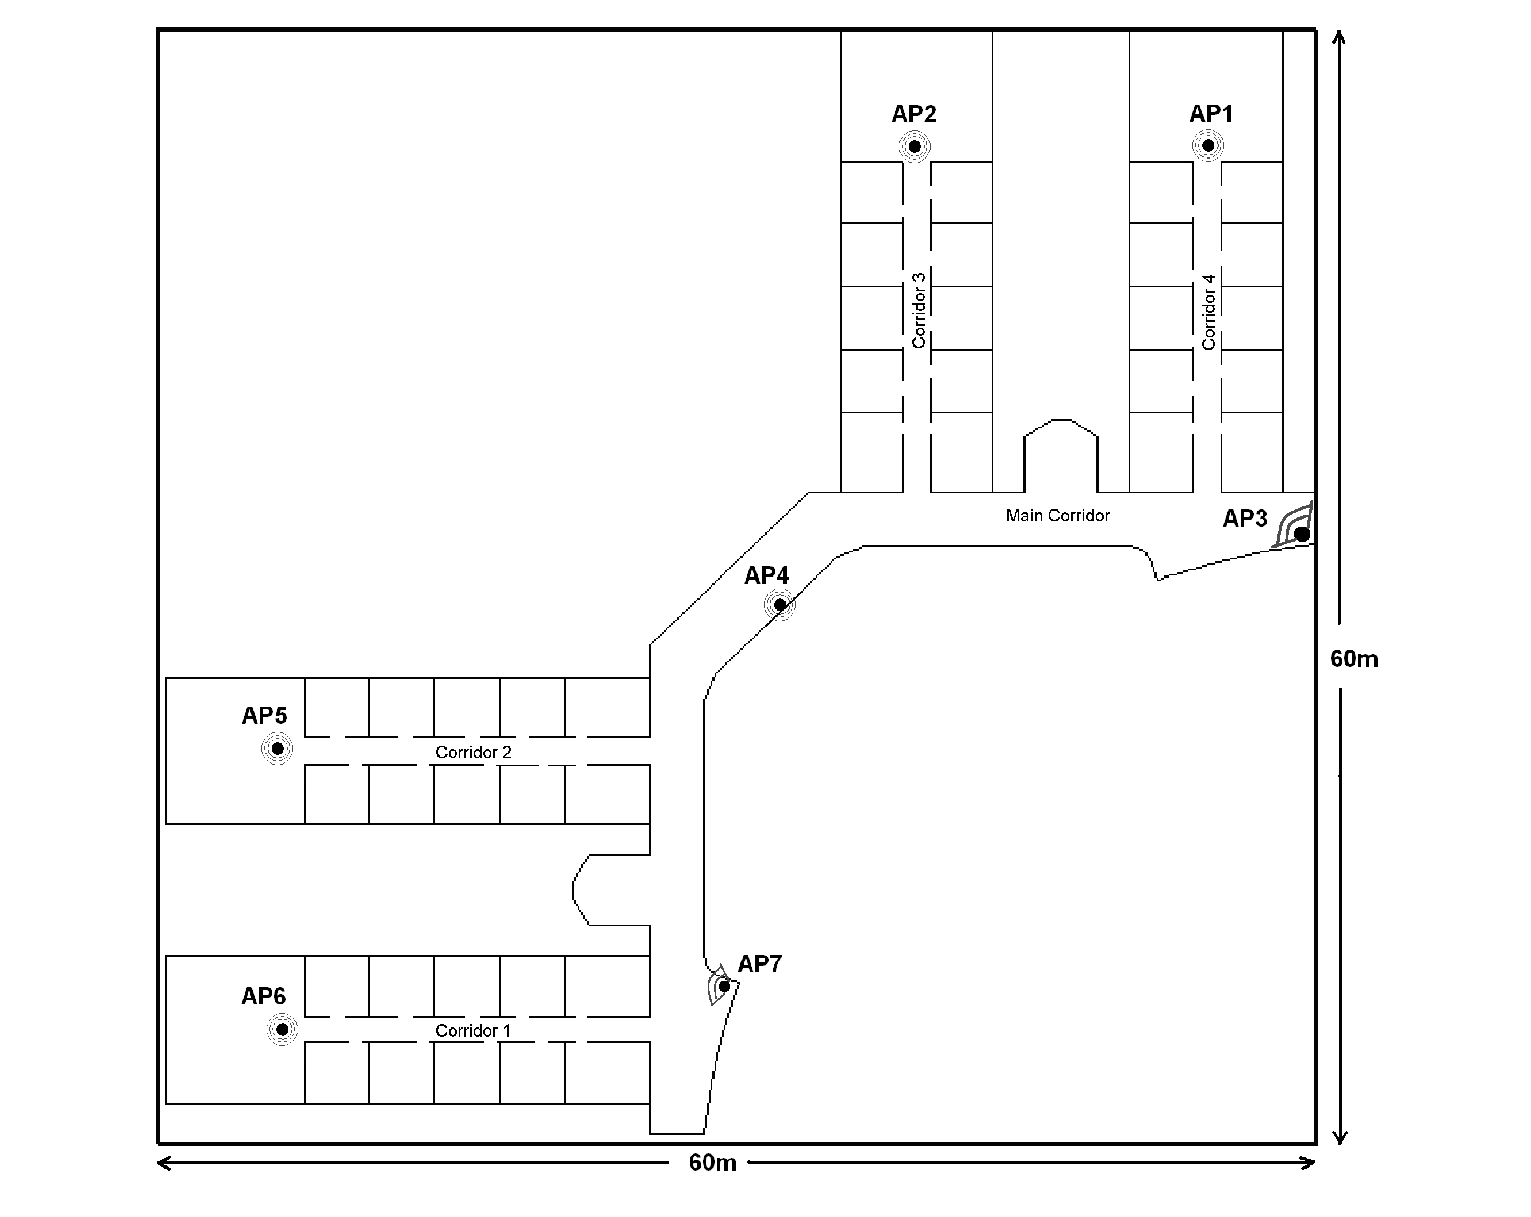
\includegraphics[width=0.55\textwidth]{Figure1}
  \ifthenelse{\equal{\myLanguage}{english}}
  {
    \caption{Example figure in the extended summary.}
  }
  {
    \caption{Ejemplo de figura en el resumen extendido.}
  }
  \label{fig:compendium-example}
\end{figure}

\begin{table}[htbp]
  \centering
  \renewcommand{\arraystretch}{1.2}
  \ifthenelse{\equal{\myLanguage}{english}}
  {
    \caption{Example comparison of experimental results.}
  }
  {
    \caption{Ejemplo de comparación de resultados experimentales.}
  }
  \label{tab:compendium-example}
  \begin{tabular}{|l|c|c|}
    \hline
    \ifthenelse{\equal{\myLanguage}{english}}{Method}{Método} &
    \ifthenelse{\equal{\myLanguage}{english}}{Metric A}{Métrica A} &
    \ifthenelse{\equal{\myLanguage}{english}}{Metric B}{Métrica B} \\
    \hline
    \ifthenelse{\equal{\myLanguage}{english}}{Baseline}{Referencia} & 0.72 & 0.68 \\
    \hline
    \ifthenelse{\equal{\myLanguage}{english}}{Proposed method}{Método propuesto} & 0.84 & 0.79 \\
    \hline
  \end{tabular}
\end{table}

%%% Local Variables:
%%% TeX-master: "../../book"
%%% End:

%%%%%%%%%%%%%%%%%%%%%%%%%%%%%%%%%%%%%%%%%%%%%%%%%%%%%%%%%%%%%%%%%%%%%%%%%%%
% Función: capítulo de ejemplo de contribuciones de la tesis de la tesis por compendio.
%
% Uso: modifica este fichero para adaptar el contenido a tu trabajo.
%%%%%%%%%%%%%%%%%%%%%%%%%%%%%%%%%%%%%%%%%%%%%%%%%%%%%%%%%%%%%%%%%%%%%%%%%%%

\ifthenelse{\equal{\myLanguage}{english}}
{
  \chapter{Thesis Contributions}
}
{
  \chapter{Contribuciones de la tesis}
}
\label{cha:compendium-contributions}

\ifthenelse{\equal{\myLanguage}{english}}
{
  \section{Overview of the Contributions}

  Present and discuss the original contributions of the thesis. Explain how the publications relate to one another, which objective each publication addresses and how their combined results constitute a unified doctoral contribution. The three fictional papers distributed with this example illustrate how to cite each included publication while discussing its contribution~\cite{garcia2026paper1,garcia2026paper2,garcia2026paper3}.

  \subsection{Relationship between the publications}

  Explain the role of each publication and the progression from the initial research question to the combined results of the thesis.

  \section{Supporting Research Material}
  \subsection{Videos and demonstrations}

  Remember that you can very easily include links to videos in the document, and that a list similar to the lists of tables, figures, or algorithms will be generated automatically. The command is defined in \texttt{Config/postamble.tex}, while the list is rendered from \texttt{cover/list-of-videos.tex}. To use it, simply include elements such as \videoLink{Feedback amplifiers: motivation}{https://youtu.be/9xXuasS8B3M} or \videoLink{Feedback amplifiers: ideal theory}{https://youtu.be/ZGMwGX7VCbg}.

  \subsection{Algorithms and source code}

  You can also include algorithms such as Algorithm~\ref{alg:restriction}, and symbols such as~\ac{xidet}.

  In addition, you can include source code listings such as the one shown in Listing~\ref{cod:sample2}.
}
{
  \section{Resumen de las contribuciones}

  Presenta y discute las contribuciones originales de la tesis. Explica cómo se relacionan las publicaciones entre sí, qué objetivo aborda cada una y cómo sus resultados combinados constituyen una contribución doctoral unificada. Los tres artículos ficticios distribuidos con este ejemplo muestran cómo citar cada publicación incluida al discutir su contribución~\cite{garcia2026paper1,garcia2026paper2,garcia2026paper3}.

  \subsection{Relación entre las publicaciones}

  Explica el papel de cada publicación y la progresión desde la pregunta inicial de investigación hasta los resultados conjuntos de la tesis.

  \section{Material de apoyo a la investigación}
  \subsection{Vídeos y demostraciones}

  Recuerda que puedes incluir muy fácilmente enlaces a vídeos en el documento y generar automáticamente un listado similar al de tablas, figuras o algoritmos. La orden se define en \texttt{Config/postamble.tex}, mientras que el listado se genera desde \texttt{cover/list-of-videos.tex}. Para usarla, basta con que incluyas elementos similares a \videoLink{Amplificadores realimentados: motivación}{https://youtu.be/9xXuasS8B3M} o \videoLink{Amplificadores realimentados: teoría ideal}{https://youtu.be/ZGMwGX7VCbg}.

  \subsection{Algoritmos y código fuente}

  Y también puedes incluir algoritmos como el algoritmo~\ref{alg:restriction}, y símbolos como~\ac{xidet}.

  Además de listados de código fuente como en el listado~\ref{cod:sample2}.

}

\begin{algorithm}
  \caption{IntervalRestriction\label{IR}}
  \label{alg:restriction}
  \DontPrintSemicolon
  % \dontprintsemicolon
  \KwData{$G=(X,U)$ such that $G^{tc}$ is an order.}
  \KwResult{$G'=(X,V)$ with $V\subseteq U$ such that $G'^{tc}$ is an
    interval order.}
  \Begin{
    $V \longleftarrow U$\;
    $S \longleftarrow \emptyset$\;
    \For{$x\in X$}{
      $NbSuccInS(x) \longleftarrow 0$\;
      $NbPredInMin(x) \longleftarrow 0$\;
      $NbPredNotInMin(x) \longleftarrow |ImPred(x)|$\;
    }
    \For{$x \in X$}{
      \If{$NbPredInMin(x) = 0$ {\bf and} $NbPredNotInMin(x) = 0$}{
        $AppendToMin(x)$}
    }
    \nl\While{$S \neq \emptyset$}{\label{InRes1}
      \nlset{REM} remove $x$ from the list of $T$ of maximal index\;\label{InResR}
      \lnl{InRes2}\While{$|S \cap ImSucc(x)| \neq |S|$}{
        \For{$ y \in S-ImSucc(x)$}{
          \{ remove from $V$ all the arcs $zy$ : \}\;
          \For{$z \in ImPred(y) \cap Min$}{
            remove the arc $zy$ from $V$\;
            $NbSuccInS(z) \longleftarrow NbSuccInS(z) - 1$\;
            move $z$ in $T$ to the list preceding its present list\;
            \{i.e. If $z \in T[k]$, move $z$ from $T[k]$ to
            $T[k-1]$\}\;
          }
          $NbPredInMin(y) \longleftarrow 0$\;
          $NbPredNotInMin(y) \longleftarrow 0$\;
          $S \longleftarrow S - \{y\}$\;
          $AppendToMin(y)$\;
        }
      }
      $RemoveFromMin(x)$\;
    }
  }
\end{algorithm}


\begin{codefloat}
\lstinputlisting[style=Cnice]{appendix/hello.c}
\caption{Ejemplo de código fuente con estilo \texttt{Cnice}, de nuevo
  con un \texttt{lstinputlisting} dentro de un \texttt{codefloat}}
\label{cod:sample2}
\end{codefloat}

%%% Local Variables:
%%% TeX-master: "../../book"
%%% End:

\ifthenelse{\equal{\myLanguage}{english}}
{
  \chapter{Conclusions and Future Work}
}
{
  \chapter{Conclusiones y líneas futuras}
}
\label{cha:compendium-conclusions}

\ifthenelse{\equal{\myLanguage}{english}}
{
  \section{Main Conclusions}
}
{
  \section{Conclusiones principales}
}

\ifthenelse{\equal{\myLanguage}{english}}
{
  Summarize the conclusions supported by the thesis as a whole, relate them to the objectives and discuss the principal limitations. Close the extended summary by identifying research directions that follow from the results.
}
{
  Resume las conclusiones sustentadas por el conjunto de la tesis, relaciónalas con los objetivos y discute las principales limitaciones. Cierra el resumen extendido identificando las líneas de investigación que se derivan de los resultados.
}

\ifthenelse{\equal{\myLanguage}{english}}
{
  \section{Limitations}

  Discuss the assumptions and practical constraints that limit the generalization of the results and should be considered when interpreting the conclusions.

  \section{Future Research Directions}
  \subsection{Immediate extensions}

  Identify improvements and experiments that follow directly from the work presented in the thesis.

  \subsection{Long-term research opportunities}

  Outline broader questions opened by the combined contributions and publications.
}
{
  \section{Limitaciones}

  Discute las hipótesis y restricciones prácticas que limitan la generalización de los resultados y deben considerarse al interpretar las conclusiones.

  \section{Líneas futuras de investigación}
  \subsection{Extensiones inmediatas}

  Identifica las mejoras y experimentos que se derivan directamente del trabajo presentado en la tesis.

  \subsection{Oportunidades de investigación a largo plazo}

  Plantea cuestiones más amplias abiertas por el conjunto de las contribuciones y publicaciones.
}

%%% Local Variables:
%%% TeX-master: "../../book"
%%% End:


% The bibliography belongs between the extended summary and the papers.
%%%%%%%%%%%%%%%%%%%%%%%%%%%%%%%%%%%%%%%%%%%%%%%%%%%%%%%%%%%%%%%%%%%%%%%%%%%
% Función: bibliografía.
%
% Uso: inclusión automática; normalmente no debes modificarlo.
% No se compila por separado.
%%%%%%%%%%%%%%%%%%%%%%%%%%%%%%%%%%%%%%%%%%%%%%%%%%%%%%%%%%%%%%%%%%%%%%%%%%%

% IMPORTANT: YOU DON'T HAVE TO EDIT THIS FILE, JUST EDIT THE bibliofiles.tex file
% IMPORTANT: YOU DON'T HAVE TO EDIT THIS FILE, JUST EDIT THE bibliofiles.tex file
% IMPORTANT: YOU DON'T HAVE TO EDIT THIS FILE, JUST EDIT THE bibliofiles.tex file
% IMPORTANT: YOU DON'T HAVE TO EDIT THIS FILE, JUST EDIT THE bibliofiles.tex file
% IMPORTANT: YOU DON'T HAVE TO EDIT THIS FILE, JUST EDIT THE bibliofiles.tex file
% IMPORTANT: YOU DON'T HAVE TO EDIT THIS FILE, JUST EDIT THE bibliofiles.tex file
% IMPORTANT: YOU DON'T HAVE TO EDIT THIS FILE, JUST EDIT THE bibliofiles.tex file
% IMPORTANT: YOU DON'T HAVE TO EDIT THIS FILE, JUST EDIT THE bibliofiles.tex file
% IMPORTANT: YOU DON'T HAVE TO EDIT THIS FILE, JUST EDIT THE bibliofiles.tex file
% IMPORTANT: YOU DON'T HAVE TO EDIT THIS FILE, JUST EDIT THE bibliofiles.tex file
% IMPORTANT: YOU DON'T HAVE TO EDIT THIS FILE, JUST EDIT THE bibliofiles.tex file
% IMPORTANT: YOU DON'T HAVE TO EDIT THIS FILE, JUST EDIT THE bibliofiles.tex file
% IMPORTANT: YOU DON'T HAVE TO EDIT THIS FILE, JUST EDIT THE bibliofiles.tex file
% IMPORTANT: YOU DON'T HAVE TO EDIT THIS FILE, JUST EDIT THE bibliofiles.tex file
% IMPORTANT: YOU DON'T HAVE TO EDIT THIS FILE, JUST EDIT THE bibliofiles.tex file
% IMPORTANT: YOU DON'T HAVE TO EDIT THIS FILE, JUST EDIT THE bibliofiles.tex file
% IMPORTANT: YOU DON'T HAVE TO EDIT THIS FILE, JUST EDIT THE bibliofiles.tex file
% IMPORTANT: YOU DON'T HAVE TO EDIT THIS FILE, JUST EDIT THE bibliofiles.tex file
% IMPORTANT: YOU DON'T HAVE TO EDIT THIS FILE, JUST EDIT THE bibliofiles.tex file
% IMPORTANT: YOU DON'T HAVE TO EDIT THIS FILE, JUST EDIT THE bibliofiles.tex file
% IMPORTANT: YOU DON'T HAVE TO EDIT THIS FILE, JUST EDIT THE bibliofiles.tex file


\ifthenelse{\equal{\bibliosystem}{biblatex}}
{
  % Use biblatex instead of bibtex

  %% Wen changing to biblatex, we could not define here the bibliography files, so that
  %% You need to edit the bibliofiles.tex file to do so

  %% % Now add all bib files to be processed
  %% \addbibresource{\myreferencespath\mybibfileOne}
  %% % \addbibresource{\myreferencespath\mybibfileTwo}
  %% % ...
  %% % \addbibresource{\myreferencespath\mybibfileN}

  \printbibliography[heading=bibintoc]


}
{
  % Use bibtex

  %\bibliographystyle{plainnat}
  %\bibliographystyle{dinat}
  %\bibliographystyle{unsrt}
  \bibliographystyle{IEEEtran}

  % The following is overly complicated because I was not able to do so in
  % another way. The problem is the bibliography command being "called"
  % from both the root and anteproyecto directories...
  %
  %%%%%%%%%%%%%%%%%%%%%%%%%%%%%%%%%%%%%%%%%%%%%%%%%%%%%%%%%%%%%%%%%%%%%%%%%%%
% Función: selección de los ficheros de bibliografía del documento.
%
% Uso: modifica este fichero para incluir las definiciones de tu trabajo.
%%%%%%%%%%%%%%%%%%%%%%%%%%%%%%%%%%%%%%%%%%%%%%%%%%%%%%%%%%%%%%%%%%%%%%%%%%%

%% Here define as many bibfiles as needed
%%
%% It is compulsory that they are named as \mybibfileOne
%% \mybibfileTwo, \mybibfileThree, ... \mybibfileTen
%%
%% If you need more than ten, you will have to edit
%% Config/preamble.tex and Book/biblio/bibliography.tex
%% to support this adition
%%
%% The file names may change at your will, but they must
%% be in the Book/biblio directory

\newcommand{\mybibfileOne}{biblio/biblio.bib}
\newcommand{\mybibfileTwo}{biblio/nobiblio.bib}
%% \newcommand{\mybibfileThree}{AudioVisualNew.bib}
%% \newcommand{\mybibfileFour}{biblio/audiotracking.bib}
%% \newcommand{\mybibfileFive}{biblio/audiovisualtracking.bib}
%% \newcommand{\mybibfileSix}{biblio/backgroungsubstraction.bib}
%% \newcommand{\mybibfileSeven}{biblio/databases.bib}
%% \newcommand{\mybibfileEight}{biblio/evalmetrics.bib}
%% \newcommand{\mybibfileNine}{biblio/facedetect.bib}
%% \newcommand{\mybibfileTen}{biblio/facedetectADABOOST.bib}
%% \newcommand{\mybibfileEleven}{biblio/facedetectmultiview.bib}
%% \newcommand{\mybibfileTwelve}{biblio/facedetectprob2d.bib}
%% \newcommand{\mybibfileThirteen}{biblio/others.bib}
%% \newcommand{\mybibfileFourteen}{biblio/skindetect.bib}
%% \newcommand{\mybibfileFifteen}{biblio/tracking.bib}
%% \newcommand{\mybibfileSixteen}{biblio/videotracking.bib}
%% \newcommand{\mybibfileSeventeen}{biblio/voiceActivityDetection.bib}
%% \newcommand{\mybibfileEighteen}{biblio/headposeextraction.bib}
%% \newcommand{\mybibfileNineteen}{biblio/AudioVisualSpeakerTracking.bib}
%% \newcommand{\mybibfileTwenty}{biblio/BibliogPFVJ.bib}
%% \newcommand{\mybibfileTwentyone}{biblio/tools.bib}
%% \newcommand{\mybibfileTwentytwo}{biblio/infrared.bib}
%% \newcommand{\mybibfileTwentythree}{}
%% \newcommand{\mybibfileTwentyfour}{}
%% \newcommand{\mybibfileTwentyfive}{}


  \newcommand{\mybibfiles}{}
  \ifdef{\mybibfileOne}
  {
  \let\oldmybibfiles\mybibfiles
  \renewcommand{\mybibfiles}{\myreferencespath\mybibfileOne}
  }
  {
  \errorYOUmustDEFINEatLEASTmybibfileOneInbibliofilesDOTtex
  }
  \ifdef{\mybibfileTwo}
  {
  \let\oldmybibfiles\mybibfiles
  \renewcommand{\mybibfiles}{\oldmybibfiles,\myreferencespath\mybibfileTwo}
  }
  {
  }
  \ifdef{\mybibfileThree}
  {
  \let\oldmybibfiles\mybibfiles
  \renewcommand{\mybibfiles}{\oldmybibfiles,\myreferencespath\mybibfileThree}
  }
  {
  }

  \ifdef{\mybibfileFour}
  {
  \let\oldmybibfiles\mybibfiles
  \renewcommand{\mybibfiles}{\oldmybibfiles,\myreferencespath\mybibfileFour}
  }
  {
  }
  \ifdef{\mybibfileSix}
  {
  \let\oldmybibfiles\mybibfiles
  \renewcommand{\mybibfiles}{\oldmybibfiles,\myreferencespath\mybibfileSix}
  }
  {
  }

  \ifdef{\mybibfileSeven}
  {
  \let\oldmybibfiles\mybibfiles
  \renewcommand{\mybibfiles}{\oldmybibfiles,\myreferencespath\mybibfileSeven}
  }
  {
  }

  \ifdef{\mybibfileEight}
  {
  \let\oldmybibfiles\mybibfiles
  \renewcommand{\mybibfiles}{\oldmybibfiles,\myreferencespath\mybibfileEight}
  }
  {
  }

  \ifdef{\mybibfileNine}
  {
  \let\oldmybibfiles\mybibfiles
  \renewcommand{\mybibfiles}{\oldmybibfiles,\myreferencespath\mybibfileNine}
  }
  {
  }

  \ifdef{\mybibfileTen}
  {
  \let\oldmybibfiles\mybibfiles
  \renewcommand{\mybibfiles}{\oldmybibfiles,\myreferencespath\mybibfileTen}
  }
  {
  }

  \ifdef{\mybibfileEleven}
  {
    \let\oldmybibfiles\mybibfiles
    \renewcommand{\mybibfiles}{\oldmybibfiles,\myreferencespath\mybibfileEleven}
  }
  {
  }

  \ifdef{\mybibfileTwelve}
  {
    \let\oldmybibfiles\mybibfiles
    \renewcommand{\mybibfiles}{\oldmybibfiles,\myreferencespath\mybibfileTwelve}
  }
  {
  }

  \ifdef{\mybibfileThirteen}
  {
    \let\oldmybibfiles\mybibfiles
    \renewcommand{\mybibfiles}{\oldmybibfiles,\myreferencespath\mybibfileThirteen}
  }
  {
  }

  \ifdef{\mybibfileFourteen}
  {
    \let\oldmybibfiles\mybibfiles
    \renewcommand{\mybibfiles}{\oldmybibfiles,\myreferencespath\mybibfileFourteen}
  }
  {
  }

  \ifdef{\mybibfileFifteen}
  {
    \let\oldmybibfiles\mybibfiles
    \renewcommand{\mybibfiles}{\oldmybibfiles,\myreferencespath\mybibfileFifteen}
  }
  {
  }

  \ifdef{\mybibfileSixteen}
  {
    \let\oldmybibfiles\mybibfiles
    \renewcommand{\mybibfiles}{\oldmybibfiles,\myreferencespath\mybibfileSixteen}
  }
  {
  }

  \ifdef{\mybibfileSeventeen}
  {
    \let\oldmybibfiles\mybibfiles
    \renewcommand{\mybibfiles}{\oldmybibfiles,\myreferencespath\mybibfileSeventeen}
  }
  {
  }

  \ifdef{\mybibfileEighteen}
  {
    \let\oldmybibfiles\mybibfiles
    \renewcommand{\mybibfiles}{\oldmybibfiles,\myreferencespath\mybibfileEighteen}
  }
  {
  }

  \ifdef{\mybibfileNineteen}
  {
    \let\oldmybibfiles\mybibfiles
    \renewcommand{\mybibfiles}{\oldmybibfiles,\myreferencespath\mybibfileNineteen}
  }
  {
  }

  \ifdef{\mybibfileTwenty}
  {
    \let\oldmybibfiles\mybibfiles
    \renewcommand{\mybibfiles}{\oldmybibfiles,\myreferencespath\mybibfileTwenty}
  }
  {
  }

  \ifdef{\mybibfileTwentyone}
  {
    \let\oldmybibfiles\mybibfiles
    \renewcommand{\mybibfiles}{\oldmybibfiles,\myreferencespath\mybibfileTwentyone}
  }
  {
  }

  \ifdef{\mybibfileTwentytwo}
  {
    \let\oldmybibfiles\mybibfiles
    \renewcommand{\mybibfiles}{\oldmybibfiles,\myreferencespath\mybibfileTwentytwo}
  }
  {
  }

  \ifdef{\mybibfileTwentythree}
  {
    \let\oldmybibfiles\mybibfiles
    \renewcommand{\mybibfiles}{\oldmybibfiles,\myreferencespath\mybibfileTwentythree}
  }
  {
  }

  \ifdef{\mybibfileTwentyfour}
  {
    \let\oldmybibfiles\mybibfiles
    \renewcommand{\mybibfiles}{\oldmybibfiles,\myreferencespath\mybibfileTwentyfour}
  }
  {
  }

  \ifdef{\mybibfileTwentyfive}
  {
    \let\oldmybibfiles\mybibfiles
    \renewcommand{\mybibfiles}{\oldmybibfiles,\myreferencespath\mybibfileTwentyfive}
  }
  {
  }

  % Do not touch this
  % The commands around the \bibliography{} command should be included if using bibtex, but
  % according to Gonzalo Corral's PR on July 2022, they break compilation in overleaf. I think
  % this should not happen if the bib files are in iso-8859-1 when using bibtex instead of
  % biber, but need to be tested (TODO)
  \inputencoding{latin1}
  \bibliography{\mybibfiles}
  \inputencoding{utf8}
}

%%% Local Variables:
%%% TeX-master: "../book"
%%% coding: utf-8
%%% End:




\ifthenelse{\equal{\myLanguage}{english}}
  {\part{Publications Included in the Compendium}}
  {\part{Publicaciones incluidas en el compendio}}
\label{part:compendium-publications}

\includecompendiumpublication[
  \ifthenelse{\equal{\myLanguage}{english}}
    {Fictional demonstration paper. Replace this text with its publication status, the doctoral candidate's contribution and any relevant reuse permission.}
    {Artículo ficticio de demostración. Sustituye este texto por su estado de publicación, la contribución del doctorando y cualquier permiso de reutilización relevante.}
]{paper-1}
 {Coffee Cups as Fiducial Markers}
 {On the Unexpected Reliability of Coffee Cups as Fiducial Markers in Indoor Video Sequences}
 {garcia2026paper1}
 {publications/paper1.pdf}

\includecompendiumpublication
 {paper-2}
 {Temporal Consistency in Human--Object Interaction}
 {Temporal Consistency in Human--Object Interaction: Why the Spoon Usually Moves Before the Mug}
 {garcia2026paper2}
 {publications/paper2.pdf}

\includecompendiumpublication
 {paper-3}
 {Reproducible Desk-Based Vision Experiments}
 {Toward Reproducible Desk-Based Vision Experiments: A Multi-Camera Study of Papers, Pens, and Other Obstacles}
 {garcia2026paper3}
 {publications/paper3.pdf}

%%% Local Variables:
%%% TeX-master: "book"
%%% End:

\fi

%%%%%%%%%%%%%%%%%%%%%%%%%%%%%%%%%%%%%%%%%%%%%%%%%%%%%%%%%%%%%%%%%%%%%%%%%%%
% Now start text and numbering for backmatter (just backpage in our
% case)
%%%%%%%%%%%%%%%%%%%%%%%%%%%%%%%%%%%%%%%%%%%%%%%%%%%%%%%%%%%%%%%%%%%%%%%%%%%
\backmatter                                       % DO NOT TOUCH THIS LINE!

%%%%%%%%%%%%%%%%%%%%%%%%%%%%%%%%%%%%%%%%%%%%%%%%%%%%%%%%%%%%%%%%%%%%%%%%%%%
% Just for TFGs at UAH right now, but kept here JIC anybody else wants
% to use it
%%%%%%%%%%%%%%%%%%%%%%%%%%%%%%%%%%%%%%%%%%%%%%%%%%%%%%%%%%%%%%%%%%%%%%%%%%%
\ThesisInstitutionalPage{cover/backpage.tex}  % EDIT this file if
                                              % required, or comment it out

\end{document}
